\documentclass[
	% -- opções da classe memoir --
	12pt,				% tamanho da fonte
	openright,			% capítulos começam em pág ímpar (insere página vazia caso preciso)
	oneside,			% para impressão em recto e verso. Oposto a oneside
	a4paper,			% tamanho do papel.
	% -- opções da classe abntex2 --
	%chapter=TITLE,		% títulos de capítulos convertidos em letras maiúsculas
	%section=TITLE,		% títulos de seções convertidos em letras maiúsculas
	%subsection=TITLE,	% títulos de subseções convertidos em letras maiúsculas
	%subsubsection=TITLE,% títulos de subsubseções convertidos em letras maiúsculas
	% -- opções do pacote babel --
	english,			% idioma adicional para hifenização
	french,				% idioma adicional para hifenização
	spanish,			% idioma adicional para hifenização
	brazil,				% o último idioma é o principal do documento
	]{abntex2}

% ---
% PACOTES
% ---

% ---
% Pacotes fundamentais
% ---
\usepackage{lmodern}			% Usa a fonte Latin Modern
\usepackage[T1]{fontenc}		% Selecao de codigos de fonte.
\usepackage[utf8]{inputenc}		% Codificacao do documento (conversão automática dos acentos)
\usepackage{indentfirst}		% Indenta o primeiro parágrafo de cada seção.
\usepackage{color}				% Controle das cores
\usepackage{graphicx}			% Inclusão de gráficos
\usepackage{microtype} 			% para melhorias de justificação
\usepackage{float}
\usepackage{algorithm}
\usepackage{algorithmic}%para pseudocódigos
\usepackage{multirow}
\usepackage{makecell}
\usepackage{longtable}
\usepackage{caption}

% ---

% ---
% Pacotes adicionais, usados apenas no âmbito do Modelo Canônico do abnteX2
% ---
\usepackage{lipsum}				% para geração de dummy text
% ---
%pacote para diagramas
\usepackage{tikz}
\usepackage{circuitikz}
\usetikzlibrary{shapes.geometric, arrows}
\usepackage{rotating}
% ---
% Pacotes de citações
% ---
\usepackage[brazilian,hyperpageref]{backref}	 % Paginas com as citações na bibl
\usepackage[alf]{abntex2cite}	% Citações padrão ABNT

\usepackage{listings}
\definecolor{cadmiumgreen}{rgb}{0.0, 0.42, 0.24}
\lstdefinestyle{default}{
  language=[Sharp]C,
  backgroundcolor=\color{white},
  basicstyle=\ttfamily\footnotesize,
  keywordstyle=\color{blue},
  commentstyle=\color{cadmiumgreen},
  stringstyle=\color{brown},
  numberstyle=\tiny\color{gray},
  numbers=left,
  stepnumber=1,
  numbersep=10pt,
  frame=single,
  framerule=0.5pt,
  rulecolor=\color{gray},
  breaklines=true,
  breakatwhitespace=true,
  tabsize=4,
  showstringspaces=false,
  captionpos=b,  
  morekeywords={::=,<,>,|}
}
\lstset{
  style=default,
  literate=
    {á}{{\'a}}1
    {é}{{\'e}}1
    {í}{{\'i}}1
    {ó}{{\'o}}1
    {ú}{{\'u}}1
    {Á}{{\'A}}1
    {É}{{\'E}}1
    {Í}{{\'I}}1
    {Ó}{{\'O}}1
    {Ú}{{\'U}}1
    {â}{{\^a}}1
    {ê}{{\^e}}1
    {î}{{\^i}}1
    {ô}{{\^o}}1
    {û}{{\^u}}1
    {Â}{{\^A}}1
    {Ê}{{\^E}}1
    {Î}{{\^I}}1
    {Ô}{{\^O}}1
    {Û}{{\^U}}1
    {ã}{{\~a}}1
    {õ}{{\~o}}1
    {Ã}{{\~A}}1
    {Õ}{{\~O}}1
    {ç}{{\c{c}}}1
    {Ç}{{\c{C}}}1
}
% ---
% CONFIGURAÇÕES DE PACOTES
% ---
\makeatletter
\renewcommand{\ALG@name}{Algor\'{i}tmo}
\renewcommand{\listalgorithmname}{Lista de \ALG@name s}
\makeatother
%% Entrada e saída do algoritmo

\renewcommand{\algorithmicrequire}{\textbf{Entrada:}}
\renewcommand{\algorithmicensure}{\textbf{Sa\'{i}da:}}

%% Variáveis

\renewcommand{\algorithmicinputs}{\textbf{entradas}}
\renewcommand{\algorithmicoutputs}{\textbf{sa\'{i}das}}
\renewcommand{\algorithmicglobals}{\textbf{globais}}
\renewcommand{\algorithmicreturn}{\textbf{retorna}}

%% Miscelânea: inicializadores e terminadores de blocos, comandos diversos

\renewcommand{\algorithmicdo}{\textbf{fa\c{c}a}}
\renewcommand{\algorithmicto}{\textbf{at\'{e}}}
\renewcommand{\algorithmicend}{\textbf{fim}}
\renewcommand{\algorithmicprint}{\textbf{imprime}}

%% Estruturas booleanas

\renewcommand{\algorithmictrue}{\textbf{verdadeiro}}
\renewcommand{\algorithmicfalse}{\textbf{falso}}

%% Estruturas e conectores lógicos

\renewcommand{\algorithmicand}{\textbf{e}}
\renewcommand{\algorithmicor}{\textbf{ou}}
\renewcommand{\algorithmicxor}{\textbf{xou}}
\renewcommand{\algorithmicnot}{\textbf{n\~{a}o}}

%% Estruturas condicionais

\renewcommand{\algorithmicif}{\textbf{se}}
\renewcommand{\algorithmicthen}{\textbf{ent\~{a}o}}
\renewcommand{\algorithmicelse}{\textbf{sen\~{a}o}}
\renewcommand{\algorithmicelsif}{\algorithmicelse\ \algorithmicif}
\renewcommand{\algorithmicendif}{\algorithmicend\ \algorithmicif}

%% Estruturas de repetição

\renewcommand{\algorithmicwhile}{\textbf{enquanto}}
\renewcommand{\algorithmicendwhile}{\algorithmicend\ \algorithmicwhile}

\renewcommand{\algorithmicfor}{\textbf{para}}
\renewcommand{\algorithmicforall}{\textbf{para todo}}
\renewcommand{\algorithmicendfor}{\algorithmicend\ \algorithmicfor}

\renewcommand{\algorithmicloop}{\textbf{loop}}
\renewcommand{\algorithmicendloop}{\algorithmicend\ \algorithmicloop}

\renewcommand{\algorithmicrepeat}{\textbf{repita}}
\renewcommand{\algorithmicuntil}{\textbf{at\'{e}}}
% ---
% Configurações do pacote backref
% Usado sem a opção hyperpageref de backref
\renewcommand{\backrefpagesname}{Citado na(s) página(s):~}
% Texto padrão antes do número das páginas
\renewcommand{\backref}{}
% Define os textos da citação
\renewcommand*{\backrefalt}[4]{
	\ifcase #1 %
		Nenhuma citação no texto.%
	\or
		Citado na página #2.%
	\else
		Citado #1 vezes nas páginas #2.%
	\fi}%
% ---

% ---
% Informações de dados para CAPA e FOLHA DE ROSTO
% ---
\titulo{DRISC-V: Uma Arquitetura Didática Integrando RISC-V Sobre RISC~I}

%"DRISC-V: Uma Implementação Didática Baseada no RISC-V e RISC~I"
%"Do RISC~I ao RISC-V: Uma Arquitetura Didática Evolutiva"
%"DRISC-V: Aprimorando Arquiteturas Didáticas com RISC-V"
%"RISC-V Didático: Uma Evolução da Arquitetura RISC~I no Logisim e System Verilog"
%"Implementação Didática de Arquiteturas Computacionais: Do RISC~I ao RISC-V"
%"Desenvolvimento de Arquiteturas Didáticas: Integração entre RISC~I e RISC-V"
%"Uma Arquitetura Didática Moderna: Da Base RISC~I ao Padrão RISC-V"
%"DRISC-V: Um Modelo de Simulação Didático Integrando RISC~I e RISC-V"

\autor{Diogo Valadares Reis dos Santos}
\local{Campos dos Goytacazes, RJ}
\data{2024}
\instituicao{%
  INSTITUTO FEDERAL DE EDUCAÇÃO, CIÊNCIA E TECNOLOGIA FLUMINENSE
  \par
  Engenharia da Computação
  \par
  Orientador: David Vasconcelos Corrêa da Silva }
\tipotrabalho{Monografia}
% O preambulo deve conter o tipo do trabalho, o objetivo,
% o nome da instituição e a área de concentração
\preambulo{Monografia apresentada ao Instituto Federal de Educação, Ciência e Tecnologia Fluminense como parte das exigências para a conclusão do Curso Bacharelado em Engenharia da Computação.}
% ---

% ---
% Configurações de aparência do PDF final

% alterando o aspecto da cor azul
\definecolor{blue}{RGB}{41,5,195}

% informações do PDF
\makeatletter
\hypersetup{
     	%pagebackref=true,
		pdftitle={\@title},
		pdfauthor={\@author},
    	pdfsubject={\imprimirpreambulo},
	    pdfcreator={LaTeX with abnTeX2},
		pdfkeywords={abnt}{latex}{abntex}{abntex2}{projeto de pesquisa},
		colorlinks=true,       		% false: boxed links; true: colored links
    	linkcolor=blue,          	% color of internal links
    	citecolor=blue,        		% color of links to bibliography
    	filecolor=magenta,      		% color of file links
		urlcolor=blue,
		bookmarksdepth=4
}
\makeatother
% ---

% ---
% Espaçamentos entre linhas e parágrafos
% ---

% O tamanho do parágrafo é dado por:
\setlength{\parindent}{1.3cm}

% Controle do espaçamento entre um parágrafo e outro:
\setlength{\parskip}{0.2cm}  % tente também \onelineskip

% ---
% compila o indice
% ---
\makeindex
% ---

% ----
% Início do documento
% ----
\begin{document}

% Seleciona o idioma do documento (conforme pacotes do babel)
%\selectlanguage{english}
\selectlanguage{brazil}

% Retira espaço extra obsoleto entre as frases.
\frenchspacing

% ----------------------------------------------------------
% ELEMENTOS PRÉ-TEXTUAIS
% ----------------------------------------------------------
% \pretextual

% ---
% Capa
% ---
\imprimircapa
% ---

% ---
% Folha de rosto
% ---
\imprimirfolhaderosto
% ---

% ---
% NOTA DA ABNT NBR 15287:2011, p. 4:
%  ``Se exigido pela entidade, apresentar os dados curriculares do autor em
%     folha ou página distinta após a folha de rosto.''
% ---

% ---
% inserir lista de ilustrações
% ---
\pdfbookmark[0]{\listfigurename}{lof}
\listoffigures*
\cleardoublepage
% ---

% ---
% inserir lista de tabelas
% ---
\pdfbookmark[0]{\listtablename}{lot}
\listoftables*
\cleardoublepage
% ---

% ---
% inserir lista de abreviaturas e siglas
% ---
\begin{siglas}
\item[DRISC] \textit{Didatic Reduced Instruction Set Computer}(Computador Didático com Conjunto de Instruções Reduzido)
\item[PC] \textit{Program Counter}(Contador de Programa)
\item[ULA] Unidade Lógica e Aritmética
\item[CPU] \textit{Central Processing Unit}(Unidade Central de Processamento)
\item[FPU] \textit{Floating-Point Processing Unit}(Unidade de Processamento de Pontos Flutuantes)
\item[GPU] \textit{Graphics Processing Unit}(Unidade de Processamento Gráfico)
\item[TPU] \textit{Tensor Processing Unit}(Unidade de Processamento de Tensores)
\item[RAM] \textit{Random Access Memory}(Memória de Acesso Aleatório)
\item[ROM] \textit{Read-Only Memory}(Memória Somente Leitura)
\item[RISC] \textit{Reduced Instruction Set Computer}(Computador com Conjunto de Instruções Reduzido)
\item[CISC] \textit{Complex Instruction Set Computer}(Computador com Conjunto de Instruções Complexo)
\item[IDE] \textit{Integrated Development Environment}(Ambiente de Desenvolvimento Integrado)
\item[BNF] \textit{Backus-Naur Form}(Forma de Backus-Naur)
\item[DLX] \textit{DeLuXe}
\item[SAP] \textit{Simple As Possible}(O mais simples possível)
\item[MIPS] \textit{Microprocessor without Interlocked Pipelined Stages}(Microprocessador sem estágios de \textit{Pipeline} interligados)
\item[FPGA] \textit{Field Programmable Gate Array}(Matriz de portas programáveis em campo)
\item[ISA] \textit{Instruction Set Architecture}(Arquitetura do Conjunto de Instruções)
\item[HDL] \textit{Hardware Description Language}(Linguagem de Descrição de Hardware)
\item[UART] \textit{Universal Asynchronous Receiver-Transmitter}(Receptor-Transmissor Assíncrono Universal)
\item[SPI] \textit{Serial Peripheral Interface}(Interface Periférica Serial)
\item[I²C] \textit{Inter-Integrated Circuit}(Circuito Inter-Integrado)
\item[ALU] \textit{Arithmetic Logic Unit}(Unidade Lógica e Aritmética)
\item[HDL] \textit{Hardware Description Language}(Linguagem de Descrição de Hardware)
\item[VHDL] \textit{VHSIC Hardware Description Language}(Linguagem de Descrição de Hardware VHSIC)
\item[SV] SystemVerilog
\end{siglas}
% ---

% ---
% inserir lista de símbolos
% ---
%\begin{simbolos}
%  \item[$ \Gamma $] Letra grega Gama
%  \item[$ \Lambda $] Lambda
%  \item[$ \zeta $] Letra grega minúscula zeta
%  \item[$ \in $] Pertence
%\end{simbolos}
% ---

% ---
% inserir o sumario
% ---
\pdfbookmark[0]{\contentsname}{toc}
\tableofcontents*
\cleardoublepage
% ---


% ----------------------------------------------------------
% ELEMENTOS TEXTUAIS
% ----------------------------------------------------------
\textual


% ----------------------------------------------------------
% Capitulo de textual
% ----------------------------------------------------------
\chapter{Introdução}
\index{elementos textuais}
\section{Problema e Contexto}
A Organização e Arquitetura de computadores é uma disciplina que explica o funcionamento de diversos componentes internos dos computadores, como estes se comunicam e como ocorre a execução de programas em baixo nível.\cite{soares_simuladores_2015}\cite[p.12]{favero_organizacao_2011}\cite{lourenco_ensino_2005}

Essa compreensão é fundamental para os alunos de computação, que frequentemente encontram desafios durante a introdução de conceitos de programação devido à falta de entendimento das abstrações físicas envolvidas. No entanto, esses conceitos costumam ser assimilados de forma mais completa à medida que os estudantes avançam para a disciplina de Arquitetura de Computadores.\cite{raabe_processadores_2006}

Segundo \citeonline{clements_arms_2010}, o conhecimento desta disciplina tem  uma grande importância no entendimento de outras áreas dentro de cursos de computação. Ao usar uma arquitetura de processador específica, os estudantes têm uma compreensão melhor de problemas no mundo real. 

Porém, como afirmado por \citeonline{djordjevic_integrated_2000} um desafio significativo no ensino dessas arquiteturas é a dificuldade de estabelecer uma conexão cognitiva entre o conhecimento teórico e a aplicação prática. Isso se agrava porque há situações em que os modelos das operações internas das arquiteturas apresentados aos alunos frequentemente estão errados ou incompletos.\cite[p.60]{yehezkel_three_2001}

Alguns professores optam por utilizar algumas arquiteturas comerciais, mas \citeonline[p.9]{clements_selecting_1999}(\citeyear{clements_arms_2010}) diz que a utilização de algumas destas arquiteturas no ensino pode complicar o trabalho do professor, pois elas geralmente são mais complexas ao tentar maximizar a entrada no mercado e o lucro das empresas que as criaram.

É possível a utilização de arquiteturas hipotéticas didáticas, mas isso pode desmotivar os alunos, que acabam sentindo que o uso destas arquiteturas não reflete problemas encontrados no mundo real. \cite{clements_arms_2010}

Uma boa solução seria a utilização de uma arquitetura didática baseada em uma arquitetura comercial, como realizado na arquitetura DLX \cite[p. 96-108]{patterson_computer_1996} que foi derivada sobre a arquitetura comercial MIPS, além de tirar inspiração de várias outras. Com uma arquitetura criada desta forma, mantém-se a vantagem de ser feita para o ensino, sendo mais simples, porém se mantendo realista ao usar como base arquiteturas reais.

O constante aumento de conteúdo na área de computação também se torna um obstáculo para o ensino. Uma possível solução é o aumentar o grau de abstração do conteúdo ensinado, no entanto, esta abstração só pode ser executada até certo nível antes que haja um prejuízo na compreensão e aprendizado dos estudantes. \cite[p.176]{wolffe_teaching_2002}

Uma boa opção para o ensino é a utilização de simuladores, pois isso permite que os estudantes visualizem os eventos que ocorrem durante a execução de um programa em diferentes níveis de abstração. Os estudantes também conseguem criar seus próprios circuitos e arquiteturas através destes simuladores, ajudando o entendimento da operação de máquinas reais.\cite[p.176-177]{wolffe_teaching_2002}

\section{Objetivos}\label{sec-objetivos}
O objetivo geral deste trabalho é implementar uma arquitetura computacional didática voltada para alunos de cursos superiores na área de computação, fazendo uso de simuladores. Essa arquitetura abrange desde o planejamento do circuito base até a criação de um \textit{assembler}. O propósito dessa implementação é fornecer um conteúdo educacional detalhado para auxiliar nos estudos, incluindo uma documentação completa da arquitetura e do processo de desenvolvimento.

Para alcançar esse objetivo é necessário completar os seguintes objetivos específicos:
\begin{enumerate}[label=\textbf{O\arabic*-}]
    \item Catalogar arquiteturas já existentes que possuam baixa complexidade e que se aproximem de arquiteturas atuais.
    \item Executar uma bibliometria sobre uma arquitetura previamente escolhida em comparação a outras.
    \item Criar e disponibilizar um modelo de simulação de uma arquitetura, utilizando como base os trabalhos encontrados.
    \item Aprimorar o modelo de simulação adicionando recursos de interesse e priorizando a clareza e a compreensão didática.
    \item Criar um \textit{assembler} para a compilação de programas específicos para a arquitetura implementada no modelo de simulação.
    \item Elaborar uma documentação didática que abranja todos os conceitos principais e os passos de criação da arquitetura.
%O7- Avaliar a arquitetura desenvolvida por meio de testes e feedback dos estudantes, fazendo ajustes conforme necessário para melhorar a %clareza e a eficácia didática.
\end{enumerate}

\section{Justificativa}
Ao final deste trabalho, espera-se obter uma arquitetura e seu modelo de simulação completo e funcional, que seja não só fácil de entender, mas que também sirva como uma ferramenta educacional robusta.

A arquitetura desenvolvida integrará recursos relevantes para o mercado atual, proporcionando aos alunos acesso a conteúdos atualizados. Além disso, será simplificada para facilitar a compreensão. O modelo de simulação proposto permitirá que os alunos experimentem e compreendam conceitos avançados de arquitetura de computadores em um ambiente interativo, controlado e acessível. 

A documentação detalhada e as ferramentas desenvolvidas servirão como um guia prático para professores e alunos, proporcionando um recurso valioso para o ensino e a aprendizagem da Arquitetura de Computadores.

Além disso, será crucial considerar a usabilidade na apresentação da arquitetura e documentação aos alunos. Se essa usabilidade for aplicada de forma adequada, a experiência de aprendizado e a motivação dos estudantes podem ser melhoradas, tornando o processo mais fácil e afetando positivamente seu progresso.\cite{dimitrijevic_usability_2020}

Portanto, uma arquitetura computacional didática bem documentada e com boa usabilidade tem valor como ferramenta de ensino em Arquitetura de Computadores. Este projeto visa proporcionar uma compreensão clara e prática dos conceitos fundamentais, preparando os alunos para suas futuras carreiras na área de computação.


\chapter{Fundamentação teórica}\label{cap_fund_teorica}

\section{Arquitetura e Organização de Computadores}

\citeonline[p.18]{tanenbaum_structured_2013} diz que o conjunto de tipos de dados, operações e recursos em todos os níveis de abstração de um computador é chamada arquitetura. A arquitetura lida com os aspectos visíveis ao usuário presente em certo nível. Aspectos de implementação como tecnologia utilizada para a produção do chip não faz parte da arquitetura.
O estudo de como desenvolver as partes de um sistema computacional que são visíveis aos programadores é chamado Arquitetura e Organização de computadores

\subsection{A Máquina de von Neumann}\label{sec:maq_von_neumann}

Segundo \citeonline[p.18]{tanenbaum_structured_2013},atualmente, a Máquina de von Neumann é a base para quase todas as arquiteturas computacionais atuais, sendo um design com enorme influência.

% Define block styles
\usetikzlibrary{positioning,calc,fit,arrows}
\tikzset{arrow/.style = {->,> = latex, line width=0.5mm, shorten >=1mm, shorten <=1mm, >={Latex[length=4mm, width=4mm]}}}

\begin{figure}[ht]
\resizebox{1\textwidth}{!}{%
\begin{circuitikz}
\tikzstyle{every node}=[font=\LARGE]

\draw  (16.25,18) rectangle  node {\hyperref[sec:memoria]{Memória}} (21.25,15.5);
\node at (12.5, 11.75) [rectangle, draw, text width=11.5em, text centered, minimum height=6em] {\hyperref[sec:control]{Unidade de Controle}};
\node at (25, 11.25) [rectangle, draw, text width=11.5em, text centered, minimum height=8.5em] {\hyperref[sec:ULA]{Unidade Lógica e Aritmética}\\\_};
\draw  (30,9.5) rectangle  node {Saída} (33.75,10.5);
\draw  (30,12) rectangle  node {Entrada} (33.75,13);

\draw [arrow] (12,13) -- (16.25,17.25);
\draw [arrow] (16.25,16.25) -- (13,13);
\draw [arrow] (24.5,13) -- (21.25,16.25);
\draw [arrow] (21.25,17.25) -- (25.5,13);
\draw [arrow] (15,12.25) -- (22.5,12.25);
\draw [arrow] (22.5,11.25) -- (15,11.25);

\draw  (22.75,10.5) rectangle  node {Acumulador} (27.25,9.5);
\draw [arrow] (30,12.5) -- (27.25,10);
\draw [arrow] (27.25,10) -- (30,10);
\end{circuitikz}
}%
\caption{A Máquina de von Neumann original\cite[p.18]{tanenbaum_structured_2013}}\label{fig:von_neumann_machine}
\end{figure}


A Máquina de von Neumann tinha 5 partes básicas: a memória, a unidade lógica e aritmética(ULA), a unidade de controle e os dispositivos de entrada e de saída. Em computadores atuais, estas 5 partes são combinadas em um chip chamado unidade central de processamento(CPU).\cite[p.18]{tanenbaum_structured_2013}

\subsection{Características de Arquiteturas de Computadores}
\subsubsection{Níveis de Máquina}\label{sec:niveis_maquina}
\citeonline[p.5]{tanenbaum_structured_2013} diz que a maioria dos computadores modernos consistem em dois ou mais níveis, como representado na Figura~\ref{fig:machineLevels}. Os níveis mais baixos estão mais próximos do \textit{hardware} real da máquina enquanto os mais altos são abstrações dos níveis abaixo, se aproximando do \textit{software}.
\begin{figure}[h!]
    \centering
    \begin{tikzpicture}[node distance=2cm]
        % Level 5
        \node (level5) [draw, rectangle, minimum width=9cm, minimum height=0.9cm] {Nível de língua orientada a problemas};
        \node (label5) [left=0.5cm of level5] {Nível 5};
        
        % Level 4
        \node (level4) [draw, rectangle, minimum width=9cm, minimum height=0.9cm, below of=level5] {Nível de linguagem \textit{assembly}};
        \node (label4) [left=0.5cm of level4] {Nível 4};
        
        % Level 3
        \node (level3) [draw, rectangle, minimum width=9cm, minimum height=0.9cm, below of=level4] {Nível de máquina do sistema operacional};
        \node (label3) [left=0.5cmof level3] {Nível 3};
        
        % Level 2
        \node (level2) [draw, rectangle, minimum width=9cm, minimum height=0.9cm, below of=level3] {Nível de arquitetura do conjunto de instruções};
        \node (label2) [left=0.5cm of level2] {Nível 2};
        
        % Level 1
        \node (level1) [draw, rectangle, minimum width=9cm, minimum height=0.9cm, below of=level2] {Nível de microarquitetura};
        \node (label1) [left=0.5cm of level1] {Nível 1};
        
        % Level 0
        \node (level0) [draw, rectangle, minimum width=9cm, minimum height=0.9cm, below of=level1] {Nível de lógica digital};
        \node (label0) [left=0.5cm of level0] {Nível 0};
        
        % Connecting lines with labels
        \draw[-] (level0) -- (level1) node[midway, right] {\textit{Hardware}};
        \draw[-] (level1) -- (level2) node[midway, right] {Interpretação(microprograma) ou execução direta};
        \draw[-] (level2) -- (level3) node[midway, right] {Interpretação parcial(Sistema Operacional)};
        \draw[-] (level3) -- (level4) node[midway, right] {Tradução (\textit{assembler})};
        \draw[-] (level4) -- (level5) node[midway, right] {Tradução (compilador)};
    \end{tikzpicture}
    \caption{Um computador de 6 níveis. O método suportado para cada nível é indicado abaixo dele(junto com o programa que suporta). \label{fig:niveisTanenbaum}\cite[Adaptação~p.5]{tanenbaum_structured_2013}}\label{fig:machineLevels}
\end{figure}
No nível mais baixo, o nível de lógica digital, se observa as portas lógicas que compõe o computador e como elas se conectam. Essas portas lógicas funcionam com entradas e saídas digitais, e realizam operações como "OU", "E" e "NÃO"; Quando combinadas entre si, essas portas lógicas podem realizar quaisquer operações matemáticas, ou podem também armazenar informações quando formam componentes chamados registradores.

O seguinte nível é o da microarquitetura.  Nesse nível temos componentes mais complexos trabalhando em conjunto. Este engloba a ULA, memória e controle, e conecta eles através de um caminho de dados(\textit{datapath}), o que permite as informações serem enviadas da memória pra ULA, que realiza alguma operação, e por fim devolve este resultado à memória.

O nível de Arquitetura do Conjunto de Instruções(ISA) contém todas instruções que a máquina pode executar, estas sendo representadas pela linguagens de máquina como sequências de números que dizem o que os componentes da máquina devem fazer. 

O próximo nível é um nível híbrido, o nível de máquina do sistema operacional, onde a maioria das instruções também está presente no nível ISA. Este nível inclui novas instruções, uma organização de memória diferente, a capacidade de executar múltiplos programas simultaneamente e outras características.  As novas funcionalidades do nível 3 são executadas por um interpretador no nível 2, chamado de sistema operacional. Algumas instruções do nível 3 são executadas diretamente pelo microprograma ou controle por hardware, enquanto outras são interpretadas pelo sistema operacional.

Os dois níveis mais altos são os que os programadores comuns geralmente usam para a resolução de problemas. Estes níveis, diferentemente dos níveis mais baixos, são suportados apenas por tradução.  Além disso, a forma com que esses programas são representados é diferente, trocando a forma numérica presente nos níveis mais baixos por uma forma mais compreensível para humanos, composto de palavras e abreviações significativas.

O 4° nível está mais diretamente conectado à linguagem de máquina, contendo a linguagem \textit{assembly}, onde cada comando individual pode ser traduzido diretamente para uma instrução nos níveis inferiores. Esta tradução se dá por um programa chamado \textit{assembler}.

Por fim, temos o 5° nível, que contém todas as linguagens em alto nível que precisam ser então traduzidas para os níveis 4 e 3 no processo chamado compilação.\cite[p.5-8]{tanenbaum_structured_2013}

\subsubsection{Barramentos}
Um barramento é um grupo físico de fios que possui uma função relacionada. Eles permitem a comunicação entre as várias partes da microarquitetura, como, por exemplo, um barramento de dados é o grupo de fios que permite a transferência de dados entre a memória e todos os subsistemas que compõem o computador.\cite[p.11-12]{catsoulis_designing_2002}
Além do barramento de dados, existem o barramento de endereços, responsável por determinar o endereço de memória que está sendo acessado pelo processador, e o barramento de controle, responsável pelos sinais de comandos, que definem o que as partes de uma máquina devem fazer.

\subsubsection{\textit{Pipeline}}
A \textit{pipeline} de instruções é uma técnica que melhora o desempenho do processador ao dividir a execução de uma instrução em várias etapas, como busca, decodificação, cálculo de operandos, busca de operandos e execução. Semelhante a uma linha de montagem, onde diferentes estágios de produção ocorrem simultaneamente, a  \textit{pipeline} permite que várias instruções sejam processadas ao mesmo tempo em diferentes estágios. No entanto, a eficiência da \textit{pipeline} pode ser afetada por fatores como o tempo de execução ser maior que o tempo de busca e instruções de desvio condicional que tornam o endereço da próxima instrução desconhecido. Para mitigar esses problemas, técnicas como a predição de desvios são utilizadas, permitindo um aumento significativo na velocidade de execução das instruções. \cite[p.47-51]{stallings_reduced_1988}

\subsubsection{Conjunto de instruções}
Segundo \citeonline[p.195]{monteiro_introducao_2007}, o conjunto de instruções (ISA) de um processador estabelece as operações básicas que a máquina executará e influencia diretamente o desempenho de suas atividades. Ele também define as especificações dos demais componentes, já que as instruções afetam praticamente todos os elementos do processador, como a ULA, os registradores e o barramento interno. O formato e os componentes das instruções determinam a organização e o desempenho do decodificador de instruções, bem como a largura do registrador de instruções.

Complementando essa perspectiva, o nível ISA é definido por como a máquina se apresenta ao programador de linguagem de máquina, ou mais realisticamente, ao compilador. Para que o compilador gere código compatível com a ISA, é necessário conhecer o modelo de memória, os registradores disponíveis, os tipos de dados suportados e o conjunto de instruções. Essa coleção de informações constitui a definição da ISA.\cite[p.345-346]{tanenbaum_structured_2013}

Assim, a partir da especificação das instruções de máquina, o restante do processador começa a ser delineado, sendo uma parte crucial do projeto de processadores e definindo sua arquitetura. Em arquiteturas modernas, a ISA é formalmente definida por documentos normativos que garantem compatibilidade entre diferentes implementações, permitindo que múltiplos fabricantes produzam chips funcionalmente idênticos.\cite[p.346]{tanenbaum_structured_2013}

Esses documentos especificam o comportamento esperado das instruções, modos de operação (como modo usuário e modo kernel), e incluem seções normativas e informativas que orientam tanto projetistas quanto desenvolvedores de compiladores. Portanto, a ISA não apenas guia o projeto físico do processador, mas também estabelece uma interface estável entre hardware e software, sendo essencial para garantir interoperabilidade, desempenho e previsibilidade na execução de programas.
\cite[p.346-347]{tanenbaum_structured_2013}

\subsubsubsection{Modos de Operação}

Em arquiteturas modernas de processadores, os Modos de Operação representam diferentes níveis de privilégio que determinam o grau de acesso que o código em execução possui sobre os recursos do sistema. Essa separação é essencial para garantir segurança, estabilidade e controle adequado do hardware, especialmente em sistemas multitarefa e com suporte a sistemas operacionais.\cite[p.9]{risc-v_risc-v_2024-1}

Os modos mais comuns incluem o modo usuário, utilizado por aplicações comuns e caracterizado por acesso restrito ao hardware; o modo supervisor, geralmente reservado ao sistema operacional, com permissões para gerenciar memória, dispositivos e interrupções; e o modo de máquina (ou modo kernel), que possui o nível mais alto de privilégio e acesso irrestrito a todos os recursos do sistema. Esse último é utilizado para inicialização, configuração de segurança e controle de ambientes protegidos.\cite[p.9]{risc-v_risc-v_2024-1}

Durante a execução normal, o processador opera em modo usuário, executando aplicações. Quando uma operação privilegiada é necessária, como acessar o disco, configurar um temporizador ou manipular registradores de controle, ocorre uma \textit{trap}, que é uma interrupção controlada que transfere a execução para um modo mais privilegiado. Essas transições podem ser verticais, quando há mudança de nível de privilégio, ou horizontais, quando ocorrem dentro do mesmo nível.\cite[p.10]{risc-v_risc-v_2024-1}

A existência de múltiplos modos permite o isolamento entre aplicações e o sistema operacional, protege contra falhas ou comportamentos maliciosos, viabiliza ambientes seguros e virtualizados, e oferece flexibilidade na execução de diferentes tipos de software. Algumas arquiteturas simplificadas podem implementar apenas o modo máquina, enquanto outras oferecem três ou mais níveis para suportar sistemas operacionais complexos e múltiplos usuários.\cite[p.10]{risc-v_risc-v_2024-1}

\subsubsection{\textit{Assembly}}
Para facilitar a programação de computadores e o entendimento de código de máquina foram criadas as linguagens \textit{assembly}, que fazem o uso de mnemônicos, como "ADD", "SUB" e "LDA", para representar as instruções que estão sendo utilizadas no programa. Diferentes famílias de processadores utilizam diferentes linguagens \textit{assembly}, geralmente possuindo apenas algumas similaridades entre si. A transformação do código assembly para instruções de máquina se dá em compiladores especiais chamados \textit{assemblers}.\cite[p.6-7]{catsoulis_designing_2002}

\section{Partes de uma Microarquitetura}
Como visto anteriormente nas seções \ref{sec:maq_von_neumann} e \ref{sec:niveis_maquina}, podemos separar a microarquitetura em diversos componentes. Cada microarquitetura pode possuir seus próprios componentes, porém eles geralmente seguem alguma variação da organização ULA-Memória-Controle.

\subsection{Unidade Lógica e Aritmética(ULA)}\label{sec:ULA}
A ULA é o circuito responsável por realizar operações matemáticas lógicas e aritméticas, como somas e subtrações, "E", "OU" e deslocamento de bits.\cite[p.60]{favero_organizacao_2011}
Alguns processadores porém, podem possuir unidades separadas para multiplicação e divisão, ou para o deslocamento de bits, como exemplo o RISC~I\cite[p.13]{catsoulis_designing_2002}

\subsubsection{IEEE 754}
O padrão IEEE 754, estabelecido pela \citeonline{ieee_ieee_1985}, define regras para a representação e manipulação de números em ponto flutuante em sistemas computacionais. Ele foi criado para padronizar operações aritméticas que antes variavam entre fabricantes, dificultando a portabilidade e confiabilidade dos programas.

Esse padrão especifica:
\begin{itemize}
    \item \textbf{Formatos de dados}: como números finitos, zeros com sinal, infinitos e valores especiais como \textit{NaN} (Não é um Número).
    \item \textbf{Precisões}: incluindo formatos binários e decimais de 16, 32, 64, 128 e até 256 bits.
    \item \textbf{Regras de arredondamento}: para garantir consistência em cálculos.
    \item \textbf{Operações aritméticas}: como soma, subtração, multiplicação, divisão e funções matemáticas.
    \item \textbf{Tratamento de exceções}: como divisão por zero, estouro e operações inválidas.
\end{itemize}

Esse componente pode ser implementado separadamente da Unidade Lógica e Aritmética (ULA), por meio de uma Unidade de Ponto Flutuante (FPU), dedicada exclusivamente ao processamento de operações em ponto flutuante, o que permite maior desempenho e precisão em cálculos científicos e gráficos.

\subsection{Memória}\label{sec:memoria}
A memória em sistemas de computação desempenha um papel crucial no armazenamento e recuperação de informações essenciais para o funcionamento do sistema. Conceitualmente, a memória é simples, atuando como um repositório de dados. Entretanto, na prática, ela se configura como um subsistema complexo, composto por diferentes tipos de memórias, integradas para garantir desempenho e eficiência.\cite[p.79]{monteiro_introducao_2007}

Segundo \citeonline[p.79-80]{monteiro_introducao_2007}, a necessidade de múltiplos tipos de memória surge da crescente disparidade entre a velocidade dos processadores e o tempo de acesso às memórias. Enquanto a capacidade de processamento aumenta rapidamente, o avanço na velocidade de acesso à memória é mais lento. Além disso, o aumento no volume de dados e no tamanho dos programas exige maior capacidade de armazenamento.

Dessa forma, torna-se impraticável criar uma única memória que seja rápida, de grande capacidade e custo acessível. Para resolver esse problema, adota-se uma hierarquia de memórias, com diferentes tipos de componentes que equilibram velocidade, capacidade e custo, otimizando o desempenho do sistema computacional.
\subsubsection{Registradores}
Segundo \citeonline[p.14]{catsoulis_designing_2002}, os registradores são as unidades internas de armazenamento de um processador. Estes se comunicam diretamente com os outros componentes internos do processador. Estes registradores podem servir para funções como:
\begin{itemize}
    \item \textbf{Acumuladores}\\
    São usados em operações aritméticas. Em algumas arquiteturas, todos os registradores podem agir como acumuladores, enquanto em outras, estes servem apenas para armazenamento.
    \item \textbf{Registradores de Estado}\\
    Servem para armazenar bits de estado que refletem resultados de operações anteriores, como zero, negativo ou interrupções.
    \item \textbf{Contadores de programa(PC)}\\
     Estes são registradores especiais que apontam para a próxima instrução a ser buscada na memória e executada pelo processador. Quando a instrução é buscada, o sistema atualiza automaticamente o PC para armazenar o endereço da próxima instrução. Assim, o PC é essencial para o controle e sequenciamento da execução dos programas.\cite{favero_organizacao_2011}
     \item \textbf{Registradores de Controle}\\
     Armazenam informações importantes para o controle, como código de operação ou resultado de sua decodificação.
\end{itemize}

\subsubsection{Memória \textit{Cache}}

Um dos maiores desafios no projeto de computadores ao longo da história tem sido desenvolver sistemas de memória capazes de fornecer operandos ao processador na mesma velocidade em que ele os processa. Com o avanço acelerado da velocidade dos processadores, as memórias principais não acompanharam esse ritmo, tornando-se relativamente mais lentas a cada geração. Essa disparidade entre a velocidade da CPU e da memória tem limitado significativamente o desempenho dos sistemas computacionais, motivando pesquisas em soluções que contornem essa limitação \cite[p.304]{tanenbaum_structured_2013}.

Os processadores modernos exigem muito dos sistemas de memória, tanto em termos de latência (tempo de resposta para fornecer um operando) quanto de largura de banda (quantidade de dados fornecidos por unidade de tempo). No entanto, essas duas características frequentemente entram em conflito: técnicas que aumentam a largura de banda tendem a elevar a latência. Por exemplo, o uso de \textit{pipelining} em sistemas de memória permite o processamento simultâneo de múltiplas requisições, mas aumenta o tempo de resposta individual de cada operação \cite[p.304]{tanenbaum_structured_2013}.

Uma das soluções mais eficazes para esse problema é o uso de \textbf{memória cache}. A cache é uma memória pequena e extremamente rápida que armazena os dados mais recentemente utilizados, permitindo acessos mais rápidos. Quando uma alta porcentagem dos dados requisitados está presente na cache, a latência efetiva do sistema de memória é significativamente reduzida \cite[p.304]{tanenbaum_structured_2013}.

\subsubsubsection{Arquitetura de Caches}

Para melhorar simultaneamente a latência e a largura de banda, é comum utilizar múltiplos níveis de cache. Um modelo básico e eficiente é o uso de caches separadas para instruções e dados, conhecido como cache dividida (\textit{split cache}). Essa abordagem permite que operações de memória sejam iniciadas de forma independente em cada cache, dobrando efetivamente a largura de banda.

Nos sistemas modernos, além das caches de instruções e dados (\textbf{L1}), há também caches de segundo nível (\textbf{L2}) e terceiro nível (\textbf{L3}). A arquitetura típica inclui:

\begin{itemize}
  \item \textbf{Cache L1}: localizada no chip do processador, com tamanho entre 16 KB e 64 KB, separada para instruções (L1-I) e dados (L1-D).
  \item \textbf{Cache L2}: geralmente unificada, com capacidade entre 512 KB e 1 MB, conectada ao chip por um caminho de alta velocidade.
  \item \textbf{Cache L3}: localizada na placa do processador, composta por alguns megabytes de SRAM, mais rápida que a memória principal (DRAM).
\end{itemize}

Essas caches são geralmente inclusivas, ou seja, os dados presentes na L1 também estão na L2, e os da L2 estão na L3 \cite[p.305]{tanenbaum_structured_2013}.

\subsubsection{Arquivo de Registradores}
O Arquivo de Registradores é um componente presente desde as primeiras arquiteturas RISC~\cite[p.7-10]{peek_vlsi_1983}, consistindo em um conjunto de registradores de uso geral disponíveis para operações durante a execução de instruções. Ele está presente em diversas arquiteturas RISC, como SPARC~\cite[p.25]{sparc_international_inc_sparc_1994}, MIPS~\cite[p.40-42]{mips_tech_llc_mips32_2016}, ARM~\cite{arm_arm_2014}, RISC-V~\cite[p.20-22]{risc-v_risc-v_2024}, entre outras.

Apesar de variações entre arquiteturas, algumas características são recorrentes: a presença de 32 registradores acessíveis por vez, a conexão fixa do primeiro registrador ao valor zero, e o uso de janelas de registradores. Este último é um mecanismo que permite que apenas uma porção dos registradores físicos esteja visível ao programador em determinado momento.

Em arquiteturas como a RISC~I~\cite[p.7-10]{peek_vlsi_1983}, o Arquivo de Registradores é dividido em múltiplas janelas sobrepostas, cada uma contendo registradores locais, de entrada e de saída. Durante chamadas de procedimentos, a janela ativa é deslocada, permitindo que os registradores de saída de uma função se tornem os de entrada da próxima, reduzindo a necessidade de operações de carga e armazenamento na memória~\cite{peek_vlsi_1983}.

Contudo, embora as janelas de registradores ofereçam acesso rápido a variáveis locais e minimizem o tráfego de memória, esse recurso tem sido gradualmente abandonado em arquiteturas mais recentes. Isso se deve à sua rigidez estrutural e ao uso potencialmente ineficiente de espaço, já que nem todas as janelas são utilizadas plenamente. Em contraste, \textit{caches} modernos permitem uma alocação dinâmica de variáveis, adaptando-se melhor ao comportamento real do programa e oferecendo suporte tanto a variáveis locais quanto globais~\cite[p.43-44]{stallings_reduced_1988}.

Além disso, com o avanço das técnicas de otimização em compiladores, tornou-se possível mapear eficientemente um número ilimitado de variáveis simbólicas em um conjunto fixo de registradores físicos. Essa abordagem reduz a necessidade de estruturas complexas como janelas de registradores, promovendo maior flexibilidade e melhor aproveitamento de espaço~\cite[p.44]{stallings_reduced_1988}.

\subsubsection{Modos de Endereçamento}
\citeonline[p.15-16]{catsoulis_designing_2002} diz que há diferentes formas que uma instrução pode referenciar um registrador ou locais de memória, estas formas sendo conhecidas como modos de endereçamento de um processador. Cada arquitetura possui suas próprias formas de endereçamento, dentre estas podemos citar\cite[p.75]{patterson_computer_1996}\cite{catsoulis_designing_2002}:
\begin{itemize}
    \item \textbf{Inerente}\\
    A instrução lida puramente com registradores.
    \item \textbf{Imediatos}\\
    A instrução possui um valor literal como um de seus operandos.
    \item \textbf{Direto ou Absoluto}\\
    Parte da instrução possui um endereço que tem acesso parcial a memória. Este modo de endereçamento é comumente utilizado para reduzir a quantidade de acessos a memória, tirando a tanto a necessidade de uma busca adicional de endereços quanto reduzindo o código ao armazenar este endereço diretamente na instrução.
    \item \textbf{Registrador Indireto}\\
    Acessa um local da memória, especificado por um endereço completo(ponteiro) que esta armazenado em um registrador.
    \item \textbf{Memória Indireto}\\
    Similar ao registrador indireto, mas neste caso, o ponteiro esta contido na memória principal ao invés de um registrador.
    \item  \textbf{Indexado}\\
    Geralmente usado para ler vetores de valores, utilizando o ponteiro contido em um registrador como base, e adicionando o valor de outro registrador para obter o valor em um índice específico.
    \item \textbf{Relativo}\\
    Este modo de endereçamento é parecido com o indexado, porém o valor base geralmente é o do contador de programas. Como exemplo, há instruções que podem utilizar o endereço do contador de programas para obter o endereço de uma instrução de pulo.
    
\end{itemize}
\subsection{Unidade de Controle}\label{sec:control}
O controlador, ou unidade de controle é a parte da microarquitetura que é responsável por comandar os outros componentes do sistema. Não há um padrão definido para o funcionamento do controle e é algo que se altera tanto com a arquitetura quanto pela implementação física da mesma. Como exemplo temos o RISC~I, que segundo \citeonline{peek_vlsi_1983}, foi implementado com 3 partes: O controle de instruções, o controle de tamanho de informações e o controlador da janela do Arquivo de Registradores. Outra possível implementação é integrar tudo em um mesmo componente de controle geral, como feito no SAP-1\cite{malvino_digital_1993}

\section{Arquitetura Berkeley RISC}
A criação das arquiteturas RISC (\textit{Reduced Instruction Set Computer}) foi um marco significativo na história da computação. O projeto foi liderado pelos professores David Patterson e Carlo H. Séquin na Universidade de Berkeley, Califórnia. Este foi iniciado com o objetivo de simplificar as arquiteturas de computadores, que estavam se tornando cada vez mais complexas. A ideia central era reduzir o conjunto de instruções para aumentar a eficiência e acelerar o processo de design.

Dois grupos de estudantes participaram do desenvolvimento das duas primeiras versões do RISC \cite{daniel_t_fitzpatrick_riscy_1982}. O grupo “Gold”, composto pelos estudantes Fitzpatrick, Foderaro, Peek, Peshkess, e Van Dyke, projetou o microprocessador RISC~I \cite{peek_vlsi_1983}, enquanto grupo “Blue”, que incluía os estudantes Katevenis e Sherburne, introduziu diversas modificações no \textit{datapath} e controle do RISC~I, resultando no RISC~II \cite{katevenis_reduced_1985}.

O RISC~I foi projetado com um conjunto pequeno de instruções, de inicialmente 31 instruções sendo expandido para 39 ao fim do seu desenvolvimento \cite{patterson_design_1982}. O RISC~I visava uma execução eficiente. A simplicidade do design permitiu que ele fosse implementado em um único chip, otimizando o uso de recursos limitados como transistores, área e consumo de energia.

O RISC~II começou a ser criado em paralelo à produção do chip do RISC~I, e introduziu um Arquivo de Registradores mais compacto, que requereu por sua vez, um sistema mais sofisticado de temporização \cite{patterson_design_1982}. Além disso, o RISC~II introduziu diversas outras mudanças significativas como um sistema de instruções privilegiadas, melhorias e inclusões de novas interrupções, reorganização das instruções e mudanças estruturais de algumas conexões do \textit{datapath}.

\subsection{RISC-V}

O RISC-V é uma arquitetura de conjunto de instruções (ISA) baseada nos princípios RISC, desenvolvida inicialmente em 2010 no Laboratório de Arquitetura de Computadores da Universidade da Califórnia, Berkeley. Diferente de seus predecessores acadêmicos, o RISC-V foi projetado com foco em extensibilidade, simplicidade e liberdade de uso, sendo disponibilizado como padrão aberto e livre de royalties, o que o torna altamente atrativo para pesquisa, ensino e aplicações comerciais.\cite[p.1]{patterson_risc-v_2016}

A arquitetura RISC-V mantém os fundamentos das arquiteturas RISC clássicas, como instruções de tamanho fixo, uso intensivo de registradores e separação clara entre instruções de carga/armazenamento e operações aritméticas. No entanto, ela introduz um sistema modular de extensões, permitindo que implementações sejam adaptadas conforme as necessidades específicas de cada projeto, desde microcontroladores até supercomputadores.\cite{risc-v_risc-v_2024}

Entre suas principais características estão:
\begin{itemize}
    \item \textbf{Base modular}: composta por um conjunto mínimo de instruções inteiras (RV32I ou RV64I), ao qual podem ser adicionadas extensões como ponto flutuante (F), multiplicação e divisão (M), instruções atômicas (A), entre outras.
    \item \textbf{Suporte a múltiplas larguras de palavra}: incluindo variantes de 32, 64 e 128 bits.
    \item \textbf{Facilidade de implementação}: projetada para ser simples de decodificar e eficiente em hardware.
    \item \textbf{Ecossistema aberto}: com ferramentas, compiladores, simuladores e núcleos de processador disponíveis publicamente.
\end{itemize}

\section{CISC \textit{versus} RISC}
As arquiteturas de processadores podem ser classificadas em duas abordagens principais: CISC (Computadores com Conjunto Complexo de Instruções) e RISC(Computadores com Conjunto Reduzido de Instruções)\cite[p.19]{catsoulis_designing_2002}, previamente discutido no tópico anterior. Cada abordagem oferece vantagens e desvantagens dependendo das exigências do sistema.

A arquitetura CISC é caracterizada por conjuntos de instruções complexas e diversificadas, capazes de realizar várias operações com uma única instrução. Essa complexidade reduzia o número de instruções necessárias, o que era vantajoso em um cenário onde a memória era cara e lenta. No entanto, essa abordagem levou a processadores mais complexos, com unidades de controle e decodificação mais lentas e maiores demandas de energia, gerando sobrecarga no design do hardware.

Por outro lado, a arquitetura RISC surgiu com a ideia de simplificar o processador, transferindo parte da complexidade para os compiladores. Processadores RISC possuem conjuntos de instruções reduzidos, otimizados para execução rápida e eficiente. Embora exijam mais instruções para realizar certas tarefas, a simplicidade da decodificação e execução resulta em um desempenho superior, com instruções que geralmente são completadas em um ou dois ciclos. Além disso, os processadores RISC utilizam grandes conjuntos de registradores e implementam uma arquitetura de carga/armazenamento, onde apenas instruções específicas acessam a memória, reduzindo o número de acessos à memória externa.

RISC também se destaca pelo uso de \textit{pipelines}, permitindo a execução simultânea de várias instruções em diferentes estágios, o que aumenta ainda mais o desempenho. Devido ao baixo consumo de energia e alta eficiência, os processadores RISC são amplamente utilizados em sistemas embarcados e de baixa potência.

Apesar dessas distinções, as arquiteturas CISC e RISC têm se aproximado ao longo do tempo, com processadores CISC adotando características de RISC, como \textit{pipelines} e simplificação de instruções, e processadores RISC~Incorporando recursos mais complexos típicos da CISC. A escolha entre essas arquiteturas depende das necessidades específicas de cada aplicação: enquanto RISC oferece vantagens em termos de eficiência energética, CISC pode ser preferível em sistemas com espaço limitado para armazenamento de programas, devido à sua maior densidade de instruções.\cite[p.19-21]{catsoulis_designing_2002}

\section{Simuladores}
Um simulador é um software com uma interface interativa que facilita a construção de modelos de simulação. Ele permite que os usuários criem modelos através de elementos básicos e os interliguem conforme o fluxo lógico do sistema. A maioria dos simuladores modernos minimiza a necessidade de programação, tornando o processo mais acessível e rápido.\cite{chwif_modelagem_2014}

Os softwares de simulação permitem a criação de modelos computacionais que representam sistemas reais. Esses modelos podem ser usados para analisar e prever o comportamento do sistema sob diferentes condições. O processo envolve a definição de parâmetros, como tempos de chegada e atendimento, e a execução do modelo para obter medidas de desempenho, como a taxa de utilização de um atendente.\cite{chwif_modelagem_2014}
\subsection{Linguagens de Descrição de Hardware (HDLs)}

As linguagens de descrição de hardware (\textit{Hardware Description Languages} — HDL) são ferramentas fundamentais para o desenvolvimento e simulação de circuitos digitais. Ao invés de utilizar esquemáticos visuais, que se tornam impraticáveis à medida que a complexidade dos circuitos aumenta, HDLs permitem representar digitalmente a estrutura e o comportamento de sistemas eletrônicos por meio de uma linguagem textual.\cite{keim_what_2020}

Essa abordagem é especialmente útil na modelagem hierárquica de circuitos, que organiza transistores em portas lógicas, portas em módulos funcionais, e assim sucessivamente. Com HDLs como VHDL e Verilog, é possível expressar essas estruturas com precisão e eficiência, facilitando a síntese e simulação do circuito em plataformas como FPGAs.

Ao contrário das linguagens de programação tradicionais, HDLs descrevem operações que ocorrem em paralelo, refletindo a natureza simultânea do funcionamento dos circuitos digitais. Isso permite que diferentes partes do hardware sejam simuladas ou executadas ao mesmo tempo, mesmo que a descrição textual siga uma ordem sequencial.\cite{keim_what_2020}

\chapter{Métodos e recursos}\label{metodos_e_recursos}
\index{sinopse de capítulo}

\section{Visão geral}
Para o desenvolvimento deste trabalho, foi necessário seguir os seguintes passos metodológicos:
\begin{enumerate}[label=\textbf{\arabic*.}]
    \item \textbf{Pesquisar arquiteturas simples e didáticas:} \\
    O primeiro passo consistiu em identificar arquiteturas relevantes que pudessem servir como base para o trabalho a ser desenvolvido. Isso requereu uma pesquisa na literatura acadêmica, livros, artigos e recursos online para encontrar essas arquiteturas.
    
    \item \textbf{Pesquisar documentação sobre a arquitetura escolhida:} \\
    Das arquiteturas pesquisadas anteriormente, uma foi escolhida para uma investigação mais aprofundada. Isso envolveu o estudo de manuais, relatórios técnicos, artigos e materiais relacionados para compreender os detalhes da arquitetura escolhida.
    
    \item \textbf{Compilar a documentação da arquitetura base:} \\
    As informações coletadas no passo anterior foram organizadas para criar uma documentação abrangente que descrevesse os componentes, instruções, registradores e fluxo de dados da arquitetura base.
    
    \item \textbf{Criar o modelo de simulação base:} \\
    Foi necessário criar uma implementação funcional da arquitetura. Isso envolveu a escolha de um software para prototipagem de circuitos lógicos e a criação dos circuitos, juntamente com anotações detalhadas do processo.
    
    \item \textbf{Criar um \textit{assembler}:} \\
    Um montador (\textit{assembler}) foi criado para traduzir a linguagem de montagem em instruções executáveis pela arquitetura. Isso foi fundamental para programar e executar códigos na arquitetura.
    
    \item \textbf{Documentar o trabalho desenvolvido:} \\
    Um registro detalhado de todas as etapas anteriores foi criado. Isso incluiu descrições das modificações feitas na arquitetura, decisões de projeto e aspectos relevantes do \textit{assembler}.

    \item \textbf{Pesquisar métodos didáticos:} \\
    Foi necessário pesquisar abordagens pedagógicas eficazes para ensinar arquitetura e organização de computadores. Isso incluiu a criação de exemplos práticos, analogias, exercícios e estudos de caso.
        
    \item  \textbf{Realizar uma bibliometria sobre arquiteturas computacionais:}\\
    Uma bibliometria ofereceu informações importantes sobre a relevância da arquitetura escolhida em comparação a outras de sua época e mais recente, de forma documentada e parametrizada.
    
    \item \textbf{Pesquisar recursos de interesse ausentes na arquitetura:} \\
    Para os próximos passos, foi necessário pesquisar recursos ou funcionalidades que não estavam presentes na arquitetura base. Isso incluiu instruções específicas, modos de endereçamento ou simplificações de componentes.
    
    \item \textbf{Listar recursos e otimizações de interesse:} \\
    Foram escolhidos os recursos a adicionar e as otimizações a aplicar. Foi importante considerar o impacto no aprendizado dos alunos ao selecionar essas melhorias, bem como a complexidade de implementação.
    
    \item \textbf{Planejar a implementação de um novo recurso:} \\
    Foi necessário traçar um plano detalhado para incorporar os recursos escolhidos à arquitetura. Isso envolveu investigar a documentação existente e criar notas sobre o processo a ser executado.
    
    \item \textbf{Implementar o recurso:} \\
    Após o planejamento, os recursos foram implementados no modelo de simulação, com modificações no \textit{assembler} caso necessário.
    
    \item \textbf{Testar o funcionamento do recurso desenvolvido:} \\
    Testes foram essenciais para garantir que os recursos funcionassem conforme o esperado. Isso envolveu casos de teste, depuração e validação.
    
    \item \textbf{Documentar o recurso adicionado:} \\
    A documentação foi incrementada com informações detalhadas sobre os novos recursos. Isso incluiu como eles funcionavam, como eram utilizados e como foram implementados na arquitetura base.
    
    \item \textbf{Consolidação da documentação da arquitetura:} \\
    Todas as documentações criadas durante o trabalho foram compiladas em um único documento. Isso incluiu a descrição da arquitetura, o \textit{assembler} e os recursos adicionados.
    
    \item \textbf{Organizar os resultados e a conclusão:} \\
    Os resultados da avaliação foram analisados, e foram tiradas conclusões sobre o projeto e finalizada a monografia.
\end{enumerate}
\clearpage
Na Figura~\ref{fig:Planejamento_Monografia} observa-se os passos previamente descritos, assim como objetivos citados na seção \ref{sec-objetivos} deste documento.
\begin{figure}
    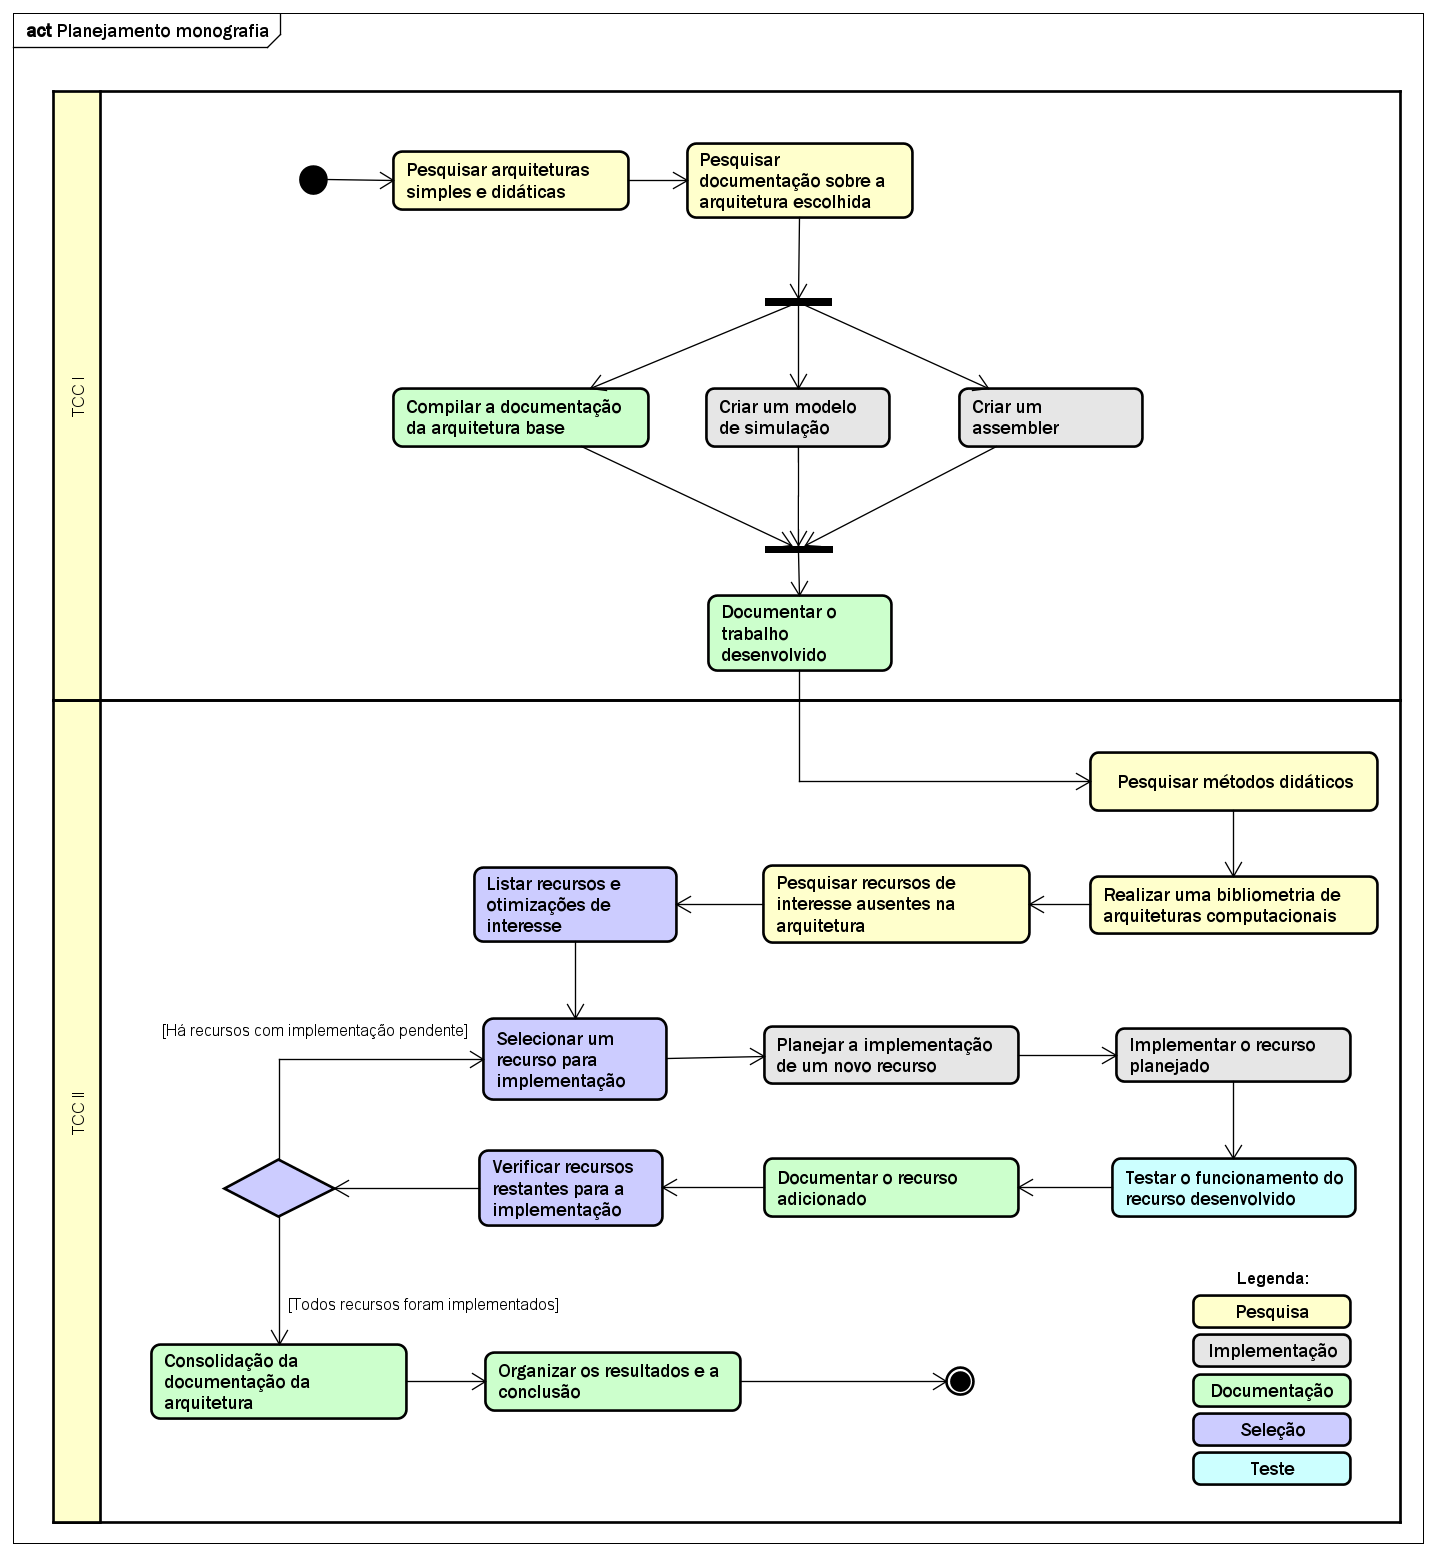
\includegraphics[width=1\linewidth]{Planejamento monografia.png}
    \caption{Planejamento Monografia}
    \label{fig:Planejamento_Monografia}
\end{figure}

\section{Ferramentas Utilizadas}
Para o desenvolvimento deste trabalho, foram utilizados diversos recursos tecnológicos que facilitaram a criação, organização e documentação do projeto. A seguir, são descritos os principais recursos empregados:

\subsection{Simulador}
Para a simulação e validação dos circuitos lógicos, foram utilizados os simuladores Logisim Evolution \citeonline{burch_logisim_2014} e Icarus Verilog \citeonline{williams_icarus_1998}. O Logisim Evolution foi empregado para a montagem visual do circuito da arquitetura, além de permitir um modelo interativo. Já o Icarus Verilog atendeu à necessidade de simulação de linguagens de descrição de hardware, proporcionando testes mais eficientes e diretos, bem como a implementação da arquitetura em FPGA.

Ambos se destacaram pela simplicidade e por serem de código aberto, possibilitando o uso sem custos adicionais e garantindo flexibilidade na modificação de funcionalidades conforme a necessidade do projeto.

\subsection{IDE e Linguagem de Programação}
Para a programação do \textit{assembler} do sistema, foi escolhida a IDE Visual Studio 2022, devido às suas ferramentas de desenvolvimento avançadas e suporte à linguagem C\# na versão .NET 8. Essa combinação facilitou a escrita, depuração e manutenção do código.

A linguagem de descrição de hardware SystemVerilog foi utilizada para modelar a arquitetura que seria executada no Icarus Verilog. Para sua programação, foi utilizado o Visual Studio Code, com a extensão Vaporview\cite(Vaporview) que oferece a visualização de formas de onda resultantes da simulação.

Por fim, o Notepad++ foi utilizado para a programação dos programas em assembly executados na arquitetura criada.

\subsection{Documentação}
A documentação do projeto foi elaborada utilizando diferentes ferramentas para atender a necessidades específicas. O \textit{Google Sheets} foi utilizado para a criação e organização de tabelas, enquanto o editor LaTeX Overleaf foi empregado na formatação e montagem do documento principal, incluindo esta monografia.

\subsection{Controle de Versão}
O controle de versão do projeto foi gerenciado através da plataforma GitHub. Esta escolha permitiu um acompanhamento detalhado das alterações no código e fácil acesso a versões anteriores do projeto, garantindo maior segurança e integridade do desenvolvimento.

\subsection{Assistentes Virtuais}
Para auxiliar na escrita dos textos da monografia e relatórios, com correções gramaticais e semânticas, foi utilizada a ferramenta Microsoft Copilot. Além disso, para otimizar a escrita de códigos, a ferramenta GitHub Copilot foi empregada, fornecendo predições automáticas de código e melhorando a eficiência do desenvolvimento.

\chapter{Trabalhos Realizados}

Durante a primeira fase de criação da monografia, uma parte significativa do trabalho foi realizada, que incluiu a criação de uma um trabalho base que pudesse ser modificado durante a fase subsequente. 

Nesta primeira fase, foram incluídas a pesquisa sobre arquiteturas viáveis para replicação e modificação, a implementação de um modelo de simulação dessa arquitetura no simulador escolhido e a criação de um \textit{Assembler} com uma linguagem que possa ser montada para a linguagem da arquitetura desenvolvida. 

Adicionalmente, foi escrita uma breve documentação, em formato de relatório técnico, detalhando como esses trabalhos foram realizado, que foram publicados abertamente na plataforma Github \cite{valadares_didactic-risc-i_2024}, acessível pelo endereço \url{https://github.com/Diogo-Valadares/Didactic-RISC-I}.

\section{Pesquisa de Arquiteturas}

O desenvolvimento de uma arquitetura didática requereu uma escolha cuidadosa de uma estrutura que fosse funcional e facilmente replicável e modificável para fins educacionais. Selecionar uma arquitetura adequada é fundamental para garantir que os conceitos possam ser ensinados de maneira clara e eficaz. Para isso, foi necessário realizar uma pesquisa abrangente que fornecesse uma visão geral das opções disponíveis, permitindo a identificação de arquiteturas que atendessem aos critérios específicos deste trabalho.

Esta seção detalha o processo realizado durante os dois primeiros passos metodológicos do trabalho: pesquisar arquiteturas simples e didáticas, e pesquisar documentação sobre a arquitetura escolhida.

\subsection{Critérios da Pesquisa}

Para iniciar esta pesquisa, foi essencial definir critérios que ajudassem a filtrar arquiteturas sem valor didático significativo ou excessivamente complexas. A simplicidade foi um fator importante, pois arquiteturas mais simples foram mais fáceis de replicar e entender. No entanto, simplicidade excessiva poderia resultar em uma falta de recursos didáticos, prolongando o processo de modificação necessário para fins educacionais.

Uma estratégia eficaz foi buscar arquiteturas mais antigas, que tendiam a ser mais simples e possuíam uma boa quantidade de documentação disponível. Arquiteturas populares entre as décadas de 70 e 90 foram analisadas, com resultados mais promissores em lançamentos pós-1980. Essas arquiteturas eram menos complexas, tornando-as mais acessíveis e também ofereciam uma base sólida de conhecimento acumulado ao longo dos anos.

Além do ano de lançamento, foram consideradas características técnicas que indicavam o nível de complexidade da arquitetura. Entre essas características estavam a largura de endereços e dados, a quantidade de instruções, a existência de uma pilha (\textit{stack}), o número de registradores, o suporte a operações de multiplicação e divisão, o suporte a números com ponto flutuante (\textit{floats}) e a utilização de \textit{pipeline}. Essas características ajudaram a determinar a adequação da arquitetura para fins didáticos, garantindo que ela fosse suficientemente robusta para ilustrar conceitos importantes sem se tornar excessivamente complexa.

Os últimos critérios foram mais subjetivos e incluíram a análise do contexto em que as arquiteturas foram utilizadas e se já tinham sido empregadas em ambientes educacionais. Saber onde e como uma arquitetura foi utilizada pôde fornecer perspectivas sobre sua relevância e aplicabilidade no ensino de conceitos de arquitetura de computadores. Arquiteturas que já foram usadas em contextos didáticos tiveram a vantagem de serem mais facilmente adaptáveis para fins educacionais. Isso ocorreu porque muitas dessas arquiteturas já eram projetadas para fins educacionais ou foram reaproveitadas de produtos comerciais como objetos de estudo. Essas arquiteturas forneceram um ponto de partida concreto para o desenvolvimento de materiais de ensino, oferecendo exemplos práticos e documentações já testadas em sala de aula.

\subsection{Metodologia de Pesquisa}

A pesquisa sobre a arquitetura base foi dividida em duas etapas: uma pesquisa geral sobre diversas arquiteturas para selecionar a mais adequada às necessidades do trabalho, seguida por uma pesquisa detalhada sobre a arquitetura escolhida, visando obter o máximo de documentação disponível.

Na primeira fase, foram realizadas pesquisas iniciais em ferramentas como Google e Microsoft Copilot para identificar superficialmente arquiteturas que atendessem aos critérios do trabalho, criando uma lista preliminar. Em seguida, essa pesquisa foi aprofundada para obter detalhes técnicos de cada arquitetura, utilizando fontes acadêmicas como Google Scholar e Periódicos Capes. Esta investigação detalhada permitiu a coleta de informações críticas e a expansão da lista com arquiteturas relacionadas às inicialmente encontradas. 

A segunda fase começou após a escolha da arquitetura e continuou durante o desenvolvimento do modelo de simulação. Pesquisas adicionais foram realizadas para preencher lacunas deixadas por estudos anteriores. Nesta etapa, além das ferramentas de busca já mencionadas, foi utilizada a ferramenta Research Rabbit para explorar trabalhos relacionados aos já encontrados. Bibliotecas digitais da Universidade de Berkeley, Califórnia, onde a arquitetura RISC~I foi desenvolvida, também foram consultadas.

\subsection{Trabalhos Encontrados}

Os trabalhos encontrados foram classificados em três categorias de importância. A primeira categoria incluiu arquiteturas que não foram relevantes para este estudo devido à sua complexidade, simplicidade excessiva ou por não atenderem a requisitos específicos. A segunda categoria abrangeu trabalhos que, embora não fossem sobre a arquitetura escolhida, eram relacionados e poderiam inspirar futuros desenvolvimentos. A última categoria consistiu em trabalhos diretamente relacionados à arquitetura selecionada. Todas as arquiteturas pesquisadas podem ser vistas na Tabela \ref{tab:relatedWork}.

\begin{table}[!htp]\centering
    \centering
    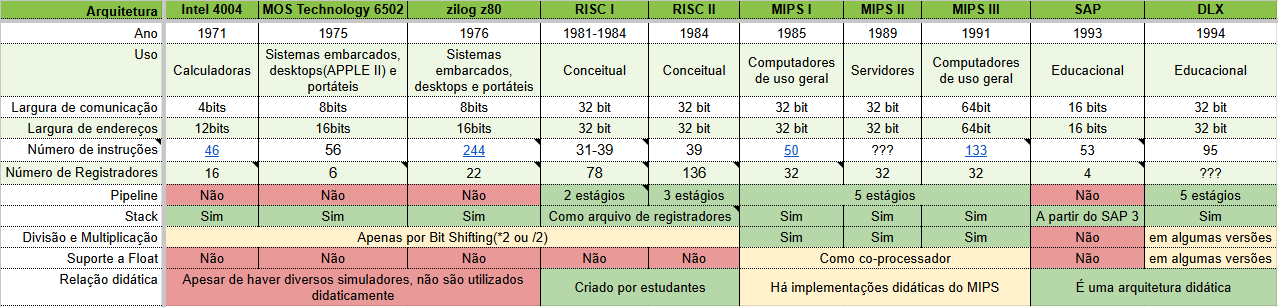
\includegraphics[width=1\linewidth]{tabelaTrabalhosRelacionados.png}
    \caption{Arquiteturas encontradas na primeira fase de pesquisa.}
    \label{tab:relatedWork}
\end{table}

Na primeira categoria, destacaram-se as arquiteturas Intel 4004 (1971), Zilog Z80 (1976) e MOS Technology 6502 (1975). Essas arquiteturas comerciais foram descartadas por serem ou muito simples ou muito complexas, além de não oferecerem conteúdo relevante para os objetivos deste trabalho.

A segunda categoria incluiu as arquiteturas SAP, MIPS e DLX. O SAP \cite{malvino_digital_1993} foi uma arquitetura teórica criada para ser a mais simples possível, ainda representando arquiteturas reais. Embora interessante, foi descartada por sua simplicidade excessiva, mas poderia servir de inspiração.

As arquiteturas MIPS e DLX \cite{patterson_computer_1996} foram exemplos de arquiteturas RISC que expandiam os conceitos do RISC~I. Apesar de serem mais complexas do que o desejado, com um \textit{pipeline} de 5 fases, ofereceram uma base sólida de conhecimento. A DLX, desenvolvida com um objetivo didático, derivou da MIPS e combinou conceitos de várias outras arquiteturas, alinhando-se bem aos requisitos deste estudo. Trabalhos relacionados à DLX, por isso, podem ser úteis como referência.

A terceira categoria foi composta por trabalhos diretamente relacionados a arquitetura escolhida, o RISC~I. O trabalho de \citeonline{peek_vlsi_1983} foi uma referência crucial, detalhando a implementação do RISC~I em um relatório técnico. Este trabalho ofereceu diagramas dos circuitos e partes da arquitetura, além da descrição do funcionamento de certos mecanismos, o que foi essencial para a replicação da arquitetura. Quase todo o modelo de simulação foi baseado neste trabalho. No entanto, muitas partes tiveram que ser decifradas ou recriadas do zero devido à falta de alguns detalhes ou às limitações do simulador em comparação à implementação física.

A dissertação de \citeonline{katevenis_reduced_1985}, embora focada no RISC~II, teve grande importância ao preencher lacunas deixadas pelo trabalho de Peek. Informações cruciais fornecidas pelo trabalho de Katevenis incluíram o funcionamento da seleção dos bytes durante instruções de carregamento e armazenamento, o funcionamento circular da janela de registradores, o gerenciamento de interrupções e o uso do registrador imediato, além de várias outras informações gerais que são comuns entre o RISC~II e o RISC~I.

Finalmente, o artigo de \citeonline{stallings_reduced_1988} sobre arquiteturas RISC contribuiu significativamente para esclarecer aspectos não abordados anteriormente. Esses aspectos incluem o pipeline, com comparações entre diferentes formas de divisão de tarefas, o formato de instrução, que não é completamente detalhado no trabalho de Peek, e a descrição de todas as instruções.

\subsection{Motivações da Escolha da arquitetura RISC~I}

O RISC~I foi escolhido por oferecer uma quantidade balanceada de recursos, não sendo difícil de entender e replicar, mas ainda complexo o suficiente para servir como uma boa base para o trabalho. A quantidade de instruções é pequena, totalizando 39 ao final do seu desenvolvimento. Muitas das instruções possuem mecanismos e ativações de controle semelhantes, o que facilitou a criação do circuito. A \textit{pipeline} do RISC~I oferece 2 fases, sendo fácil de entender, e, caso necessário, algumas pequenas alterações podem aumentar esse número para 3 fases, conforme implementado no RISC~II.\cite{katevenis_reduced_1985}

A arquitetura utiliza tanto largura de endereços quanto de dados de 32 bits, sendo similar a arquiteturas mais atuais. No quesito de operações matemáticas, o RISC~I não oferece muitas opções, contendo apenas algumas operações lógicas, soma e subtração. Apesar disso, operações adicionais como multiplicação, divisão ou operações com ponto flutuante podem ser adicionadas facilmente, tanto pelas facilidades do simulador quanto pelo espaço para expansão no conjunto de instruções.\cite{peek_vlsi_1983}

Outro recurso que o RISC~I apresenta é a janela de registradores, que, embora não seja exatamente uma pilha (\textit{stack}), possui uma função bem similar, além de ser um recurso interessante para apresentação didática. Esta janela de registradores acelera o processamento de programas no RISC~I, reduzindo a necessidade de acesso à memória primária do sistema\cite{peek_vlsi_1983}. No entanto, durante a segunda fase deste trabalho, esse recurso foi deprecado por razões que serão explicadas posteriormente.

Esta arquitetura foi criada por estudantes em um meio acadêmico, demonstrando ser uma boa opção para uso didático. Além disso, o RISC~I foi uma arquitetura altamente influente, servindo de referência para diversas arquiteturas atuais, como as arquiteturas ARM, sendo um ótimo ponto de entrada para quem deseja aprender estas arquiteturas.\cite{tanenbaum_structured_2013}

\section{Modelo de Simulação Base}\label{sec:modeloSim}

A criação de um modelo de simulação base foi um dos passos metodológicos executados. O modelo desenvolvido possui todas as funcionalidades da arquitetura RISC~I. Apesar de ter recebido modificações em relação à implementação original, devido a limitações do simulador e à falta de informações, não houve diferenças práticas no funcionamento geral do sistema.

\begin{figure}[h]
    \centering
    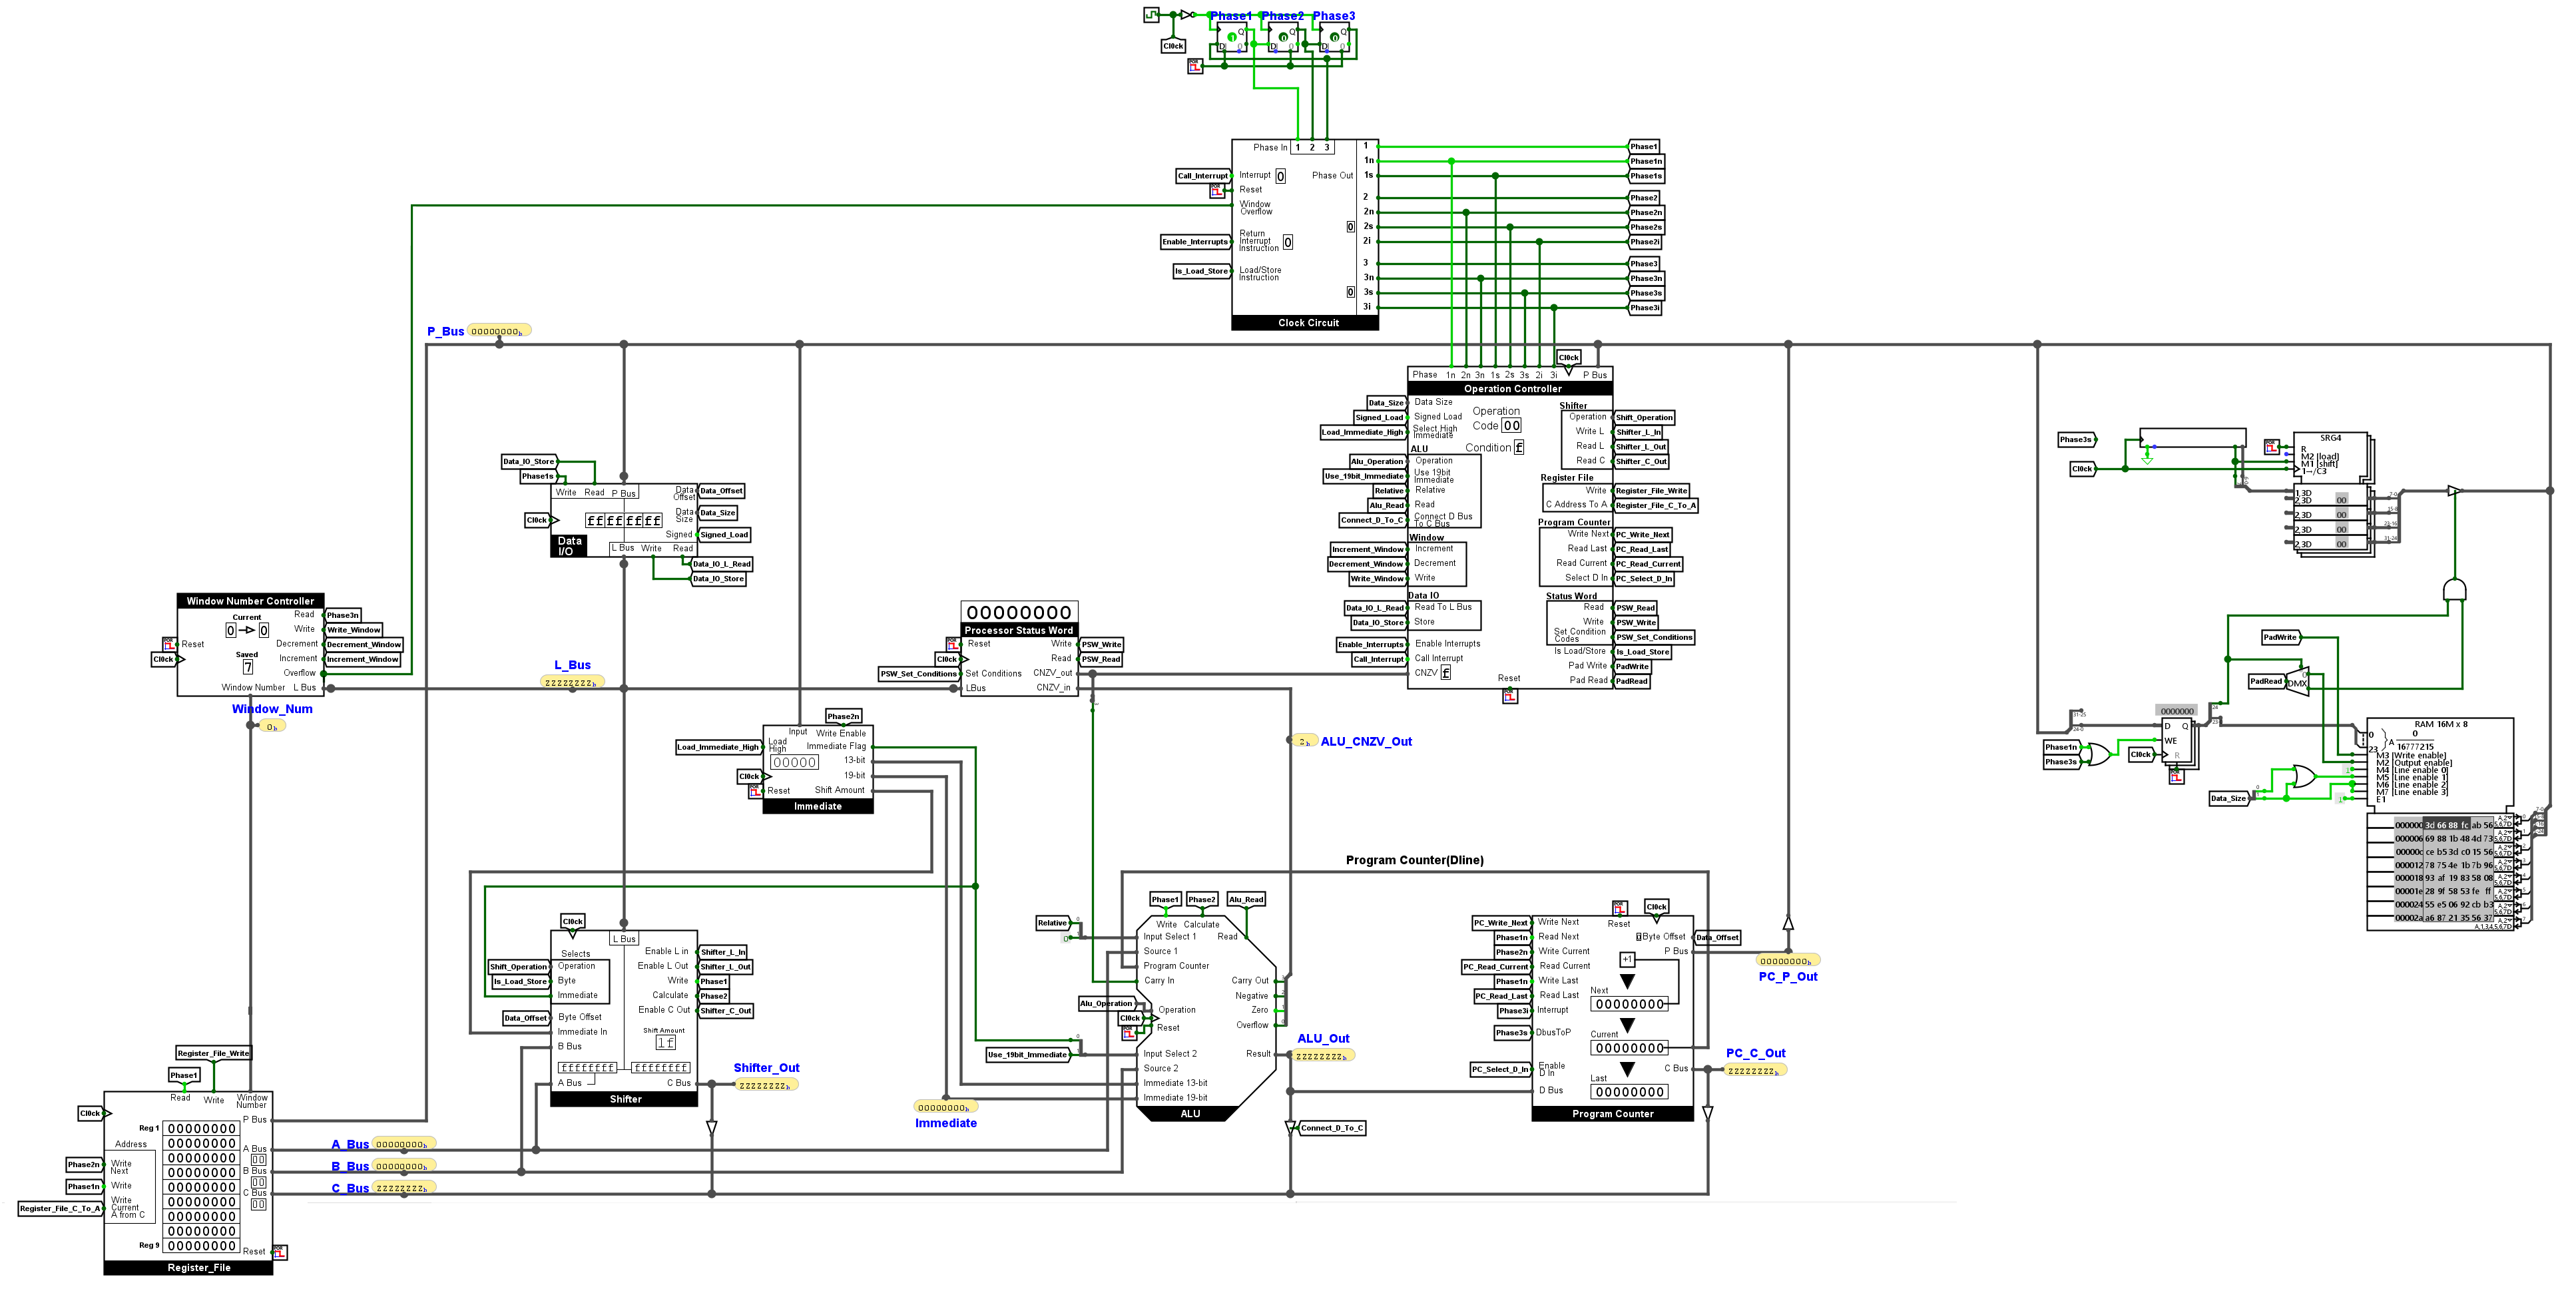
\includegraphics[width=1\linewidth]{riscInternal.png}
    \caption{Modelo de simulação no Logisim Evolution.}
    \label{fig:simModel}
\end{figure}

A Figura~\ref{fig:simModel} mostra o modelo criado com todos os seus componentes. Para a execução de programas, os programas compilados podem ser carregados diretamente na memória RAM do sistema. A possibilidade de carregar programas diretamente no modelo de simulação simplificou seu teste e desenvolvimento. Na sua versão atual, o modelo não possui nenhum componente ou tela para exibir a saída de informações, sendo necessário observar diretamente o que está sendo gravado na memória e outros componentes para verificar seu funcionamento.

Um componente adicional que foi inserido no sistema é um componente para entrada de teclado, que grava informações inseridas pelo usuário e que podem ser acessadas pelo resto do sistema. A implementação deste componente é rudimentar, servindo apenas como prova de conceito, mas pode ser aprimorada nas etapas seguintes de desenvolvimento do modelo, permitindo uma interação direta com o sistema sem a necessidade de manipulação da memória.

Apesar de o modelo de simulação estar completo, devido a limitações de tempo no desenvolvimento, não foi possível criar uma rotina de tratamento de \textit{overflow} do contador de número da janela de registradores, um componente essencial para a execução de programas que exigem chamadas de funções na memória. Esta rotina, implementada na memória do sistema como um programa, permite que mais instruções de chamadas sejam realizadas sem sobrescrever e perder dados, garantindo que o usuário não precise interferir diretamente no seu programa criado.

Completando este passo metodológico, pode-se considerar o modelo de simulação um sucesso, apesar de algumas melhorias possíveis. Este modelo servirá como uma base sólida para o desenvolvimento de um novo modelo, objetivo da próxima etapa deste trabalho. As melhorias necessárias serão implementadas ao longo desse processo, garantindo que a arquitetura criada funcione como um ponto de partida eficiente para a criação de uma arquitetura didática e seu modelo de simulação.

\section{\textit{Assembler} Base}

De forma paralela à criação do modelo de simulação, foi desenvolvido um \textit{assembler} para facilitar a criação de programas a serem testados no modelo de simulação. Assim como o modelo de simulação, essa versão do \textit{assembler} serviu como base para desenvolvimentos futuros, sendo necessário modificá-lo conforme o trabalho progredia.

Em sua primeira versão, o \textit{assembler} foi capaz de traduzir todas as instruções da linguagem \textit{assembly} criada para gerar código de máquina compatível com o RISC~I. Além disso, o \textit{assembler} possuía recursos como criação de variáveis, criação de rótulos (\textit{labels}) para endereços e suporte a números hexadecimais.

A sintaxe aceita pelo \textit{assembler} pode ser expressa pela seguinte notação BNF:

\begin{lstlisting}
<instrução> ::= <formato1> | <formato2> | <rotulo> | <declaracaoPalavra>

<formato1> ::= <mnemônico> <registradorCondicao> <registrador> <registradorValor>

<formato2> ::= <mnemônico> <registradorCondicao> <valor>

<rotulo> ::= ":" <enderecoDeRotulo>

<declaracaoPalavra> ::= ".word" [a-zA-Z][a-zA-Z0-9]* <valor>

<mnemônico> ::= "CALLI" | "CALL" | "JMP" | "CALLR" | "JMPR" | "SLL" | "GETPSW" | "SRL" | "PUTPSW" | "SRA" | "LDBU" | "LDRBU" | "LDBS" | "LDRBS" | "LDW" | "LDRW" | "LDSU" | "LDRSU" | "LDSS" | "LDRSS" | "STS" | "STRS" | "STB" | "STRB" | "STW" | "STRW" | "AND" | "XOR" | "OR" | "SUB" | "SUBC" | "SUBR" | "SUBCR" | "ADD" | "ADDC" | "RET" | "RETI" | "GETLPC" | "LDHI"

<registradorCondicao> ::= <registrador> | <condição>

<registrador> ::= "R" <número> | "r" <número>

<registradorValor> ::= <registrador> | <valor>

<valor> ::= <número> | "#" <númeroHexadecimal> | ":" <enderecoDeRotulo> | "." <enderecoDePalavra>

<condição> ::= "NEVER" | "GREATER" | "LESS_EQUAL" | "GREATER_EQUAL" | "LESS" | "HIGHER" | "LOWER_SAME" | "CARRY_CLEAR" | "LOWER" | "CARRY_SET" | "HIGHER_OR_SAME" | "POSITIVE" | "NEGATIVE" | "NOT_EQUAL" | "EQUAL" | "OVERFLOW_CLEAR" | "OVERFLOW_SET" | "ALWAYS" | "NEV" | "GT" | "LE" | "GE" | "LT" | "HI" | "LOS" | "NC" | "LO" | "C" | "HIS" | "PL" | "MI" | "NE" | "EQ" | "NV" | "V" | "ALW"

<número> ::= [0-9]+

<númeroHexadecimal> ::= [0-9a-fA-F]+

<enderecoDeRotulo> ::=[a-zA-Z][a-zA-Z0-9]*

<enderecoDePalavra> ::= [a-zA-Z][a-zA-Z0-9]*
\end{lstlisting}

Para utilizar o \textit{assembler}, um arquivo .asm contendo o código do programa deve estar presente na pasta onde o \textit{assembler} foi configurado. Ao ser executado, o \textit{assembler} mostra todos os arquivos presentes e solicita a seleção de um para compilação. Mensagens de depuração de erros são exibidas e, ao final, o resultado é mostrado e gravado em disco. Este resultado pode então ser carregado diretamente no modelo de simulação, conforme descrito na Seção \ref{sec:modeloSim}.

\section{Relatório Técnico}

Um Relatório Técnico no contexto acadêmico é um documento que detalha os métodos, resultados e conclusões de um projeto ou pesquisa. Na área de computação e arquitetura e organização de computadores, ele aborda desde a descrição de arquiteturas e algoritmos até a análise de desempenho e implementação de sistemas. Este modelo foi adotado por \cite{peek_vlsi_1983} em sua apresentação do RISC~I, o que inspirou a utilização deste modelo para a criação da documentação do que foi feito para este trabalho.

O relatório técnico criado, intitulado "Uma Implementação do RISC-I utilizando o simulador Logisim Evolution", focou em mostrar as diferenças de implementação entre a implementação original do RISC~I e a implementação realizada no Logisim. Também foram detalhados alguns aspectos do RISC~I além da implementação do \textit{assembler}. Diferentemente de um artigo, um relatório técnico não possui normas técnicas exatas a serem seguidas, o que facilitou e acelerou o processo de escrita. No entanto, foram mantidos alguns padrões da norma ABNT de artigo para garantir que o documento permanecesse organizado.

Diversas partes do relatório técnico serviram de base para a documentação didática que foi criada nos próximos passos da monografia. Além disso, o relatório pode ser facilmente adaptado para uma publicação formal, caso haja interesse. Uma das grandes motivações para a realização deste relatório técnico foi a necessidade de documentar o que foi feito de maneira detalhada e precisa, o que se encaixa perfeitamente no último passo metodológico realizado durante o TCC 1.

\section{Bibliometria sobre arquiteturas}\label{bibliometry}

O primeiro passo da segunda parte deste trabalho foi a criação de um artigo intitulado "Uma Webibliometria Sobre a Relevância de Arquiteturas Computacionais" \\ \cite{valadares_uma_2025}. Esta bibliometria foi realizada com base no trabalho de \citeonline{costa_modelo_2010}, porém com algumas alterações, sendo a maior delas a mudança na forma de pesquisa dos termos, resultando na utilização de dois tipos diferentes de pesquisa.

O primeiro tipo de pesquisa envolveu o uso da ferramenta \textit{Google Ngram Viewer}, que implementa o trabalho de \citeonline{lin_syntactic_2012}. Em resumo, esta ferramenta permite a visualização da frequência do uso de um n-gram ao longo do tempo, onde n-gram é um conjunto de n palavras, números, símbolos e outros termos, com um limite de até 5 termos por n-gram. Esta pesquisa ofereceu uma visualização da relevância e popularidade de diversas arquiteturas ao longo dos anos, mas não permitiu uma comparação direta entre as arquiteturas pesquisadas devido à sua precisão e a certos problemas na filtragem\cite{valadares_uma_2025}.

O segundo tipo de pesquisa foi similar ao de \citeonline{costa_modelo_2010}, porém com foco na pesquisa das arquiteturas em apenas duas bases de dados, o \textit{Google Scholar} e o Periódicos CAPES, aplicando diferentes formas de filtragem e tabulando a quantidade de resultados. O objetivo dessa segunda pesquisa foi obter uma forma de comparação da relevância entre arquiteturas, complementando questões que não puderam ser analisadas durante a primeira pesquisa.

A Figura~\ref{fig:ngram} mostra o resultado da pesquisa das arquiteturas no \textit{Google Ngram Viewer}, enquanto as Tabelas \ref{fig:scholar} e \ref{fig:scholarProx} apresentam os resultados das pesquisas no \textit{Google Scholar}. A Tabela \ref{fig:scholarProx} exibe uma porcentagem correspondente à quantidade de resultados com filtragem utilizando termos adicionais em relação aos resultados sem filtragem.

\begin{figure}[t]
    \centering
    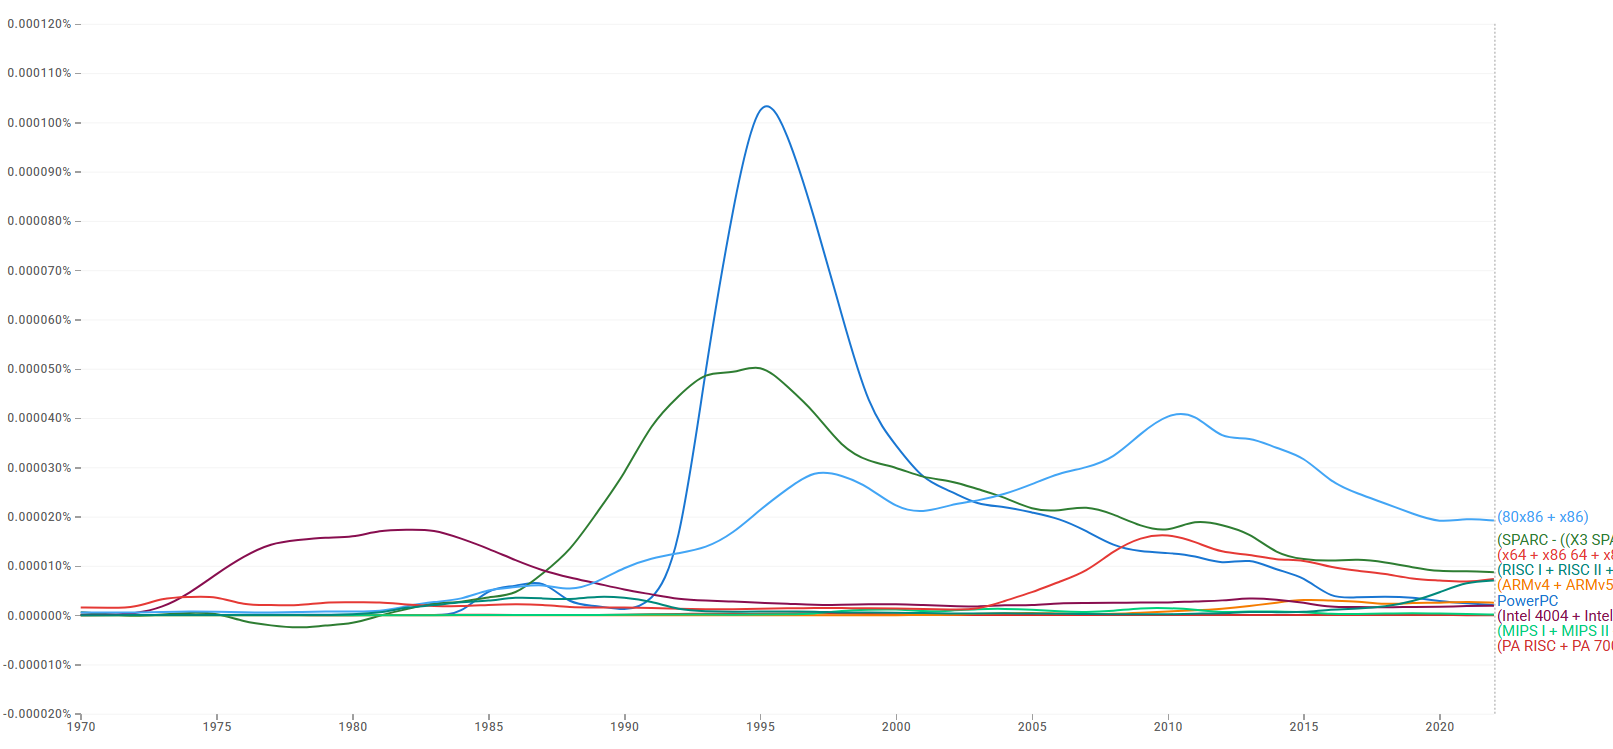
\includegraphics[width=0.86\linewidth]{Webibliometria/full.png}
    \caption{Resultado das pesquisas no \textit{Google Ngram Viewer} \cite{valadares_uma_2025}}
    \label{fig:ngram}
\end{figure}
\begin{table}[t]
    \centering
    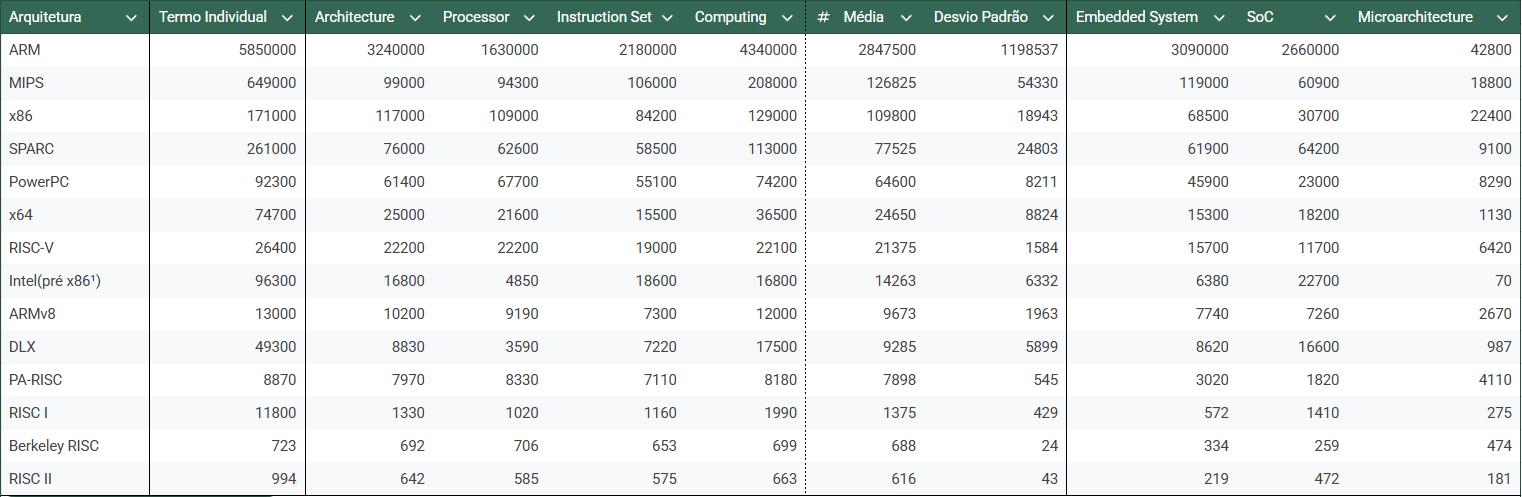
\includegraphics[width=0.86\linewidth]{Webibliometria/scholar.png}
    \caption{Resultado das pesquisas do nome da arquitetura com termos adicionais para filtragem no \textit{Google Scholar}\cite{valadares_uma_2025}}
    \label{fig:scholar}
\end{table}
\begin{table}[t]
    \centering
    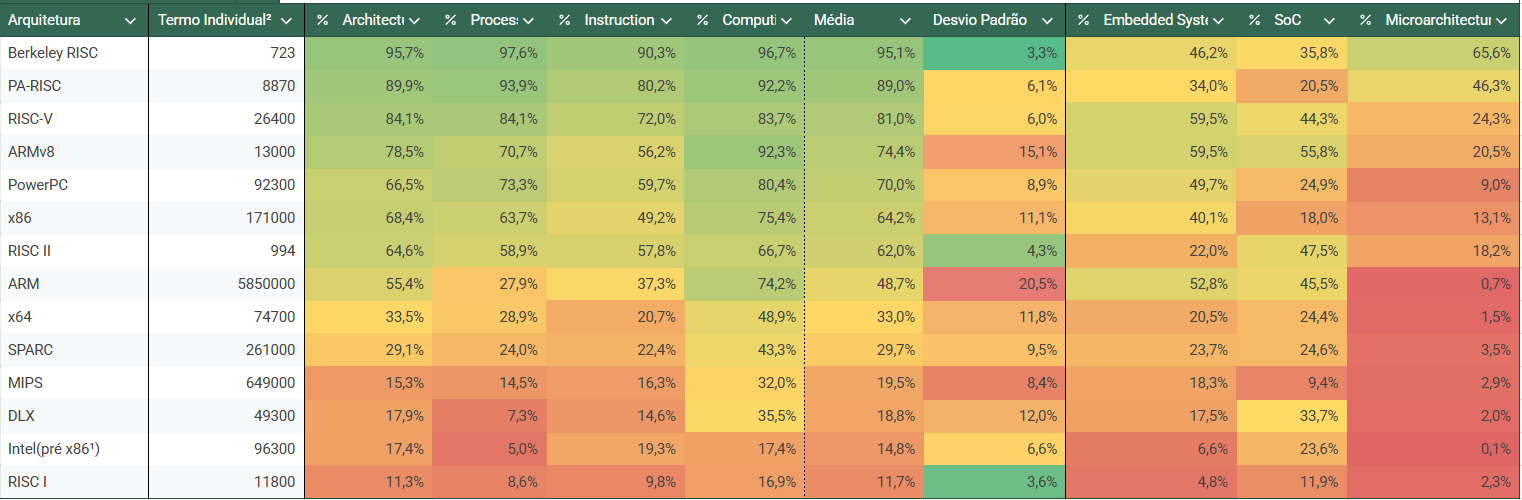
\includegraphics[width=0.86\linewidth]{Webibliometria/scholarProx.png}
    \caption{Resultado relativo das pesquisas do nome da arquitetura com termos adicionais para filtragem no \textit{Google Scholar}\cite{valadares_uma_2025}}
    \label{fig:scholarProx}
\end{table}

Após finalizada, a bibliometria ofereceu uma visão geral sobre a popularidade de algumas arquiteturas, o que permitiu uma escolha mais fácil de possíveis inspirações. Dentre as arquiteturas, duas se destacaram: ARM e RISC-V.

A família de arquiteturas ARM está consolidada em uma grande parte do mercado, totalizando cerca de 50\% de todos os processadores disponíveis mundialmente \cite{arm_building_nodate}. As arquiteturas ARM também são RISC \cite{arm_arm_2014}, tornando-as relevantes para este trabalho devido a algumas semelhanças com a arquitetura Berkeley RISC utilizada no circuito base. Apesar disso, é uma arquitetura comercial que não é aberta, o que poderia dificultar o seu uso acadêmico.

Já o RISC-V \cite{risc-v_risc-v_2024} não é exatamente uma arquitetura, mas um padrão aberto que especifica um conjunto de instruções modular. Apesar de não ser um padrão da indústria para computadores comerciais ou dispositivos móveis atualmente, ele tem ganhado rapidamente popularidade nos últimos anos devido à sua proposta, sendo já implementado em diversos microcontroladores e recebendo atualizações contínuas.

O padrão RISC-V é sucessor das arquiteturas Berkeley RISC (RISC~I, RISC~II, SOAR e SPUR \cite[p.10]{risc-v_risc-v_2024}), surgindo também na Universidade de Berkeley, mas logo se tornando uma entidade própria.

A proposta do RISC-V é descrita em seu manual:
\vspace{1.5cm} % Espaço de 1,5 cm entre o texto e a citação
\begin{adjustwidth}{4cm}{0cm} % Recuo de 4 cm da margem esquerda
\fontsize{10pt}{12pt}\selectfont

RISC-V (pronunciado "risk-five") é uma nova arquitetura de conjunto de instruções (ISA) que foi originalmente projetada para apoiar a pesquisa e a educação em arquitetura de computadores, mas que agora esperamos que também se torne um padrão livre e aberto para implementações industriais. Nossos objetivos ao definir o RISC-V incluem:

\begin{itemize}
    \item Uma ISA completamente aberta que esteja livremente disponível para a academia e a indústria.
    \item Uma ISA real adequada para implementação direta em hardware nativo, não apenas simulação ou tradução binária.
    \item Uma ISA que evita "super-arquiteturas" para um estilo particular de microarquitetura (por exemplo, microcódigo, in-order, desacoplado, out-of-order) ou tecnologia de implementação (por exemplo, full-custom, ASIC, FPGA), mas que permita uma implementação eficiente em qualquer uma dessas.
    \item Uma ISA separada em uma pequena ISA base de inteiros, utilizável por si só como base para aceleradores personalizados ou para fins educacionais, e extensões padrão opcionais, para suportar o desenvolvimento de software de uso geral.
    \item Suporte para o padrão IEEE-754 de 2008 revisado para ponto flutuante. (ANSI/IEEE Std 754-2008, IEEE Standard for Floating-Point Arithmetic, 2008)
    \item Uma ISA que suporta extensões ISA extensivas e variantes especializadas.
    \item \textbf{[...]}
\end{itemize}
\cite{risc-v_risc-v_2024}.
\end{adjustwidth}

Esta proposta e os objetivos mostrados se alinham com os objetivos e passos metodológicos deste trabalho, e por isso o RISC-V foi escolhido como padrão principal a ser seguido durante a segunda fase deste trabalho.

\section{Listagem de Recursos Para Implementação}\label{recursosMelhorias}

Antes de começar a modificar a arquitetura base, foi feita uma listagem de possíveis recursos e melhorias, que pode ser vista nas tabelas \ref{RecursosMelhoriasArquitetura} e \ref{RecursosMelhoriasAssembler}. Essas listas foram montadas observando recursos das arquiteturas pesquisadas ao longo deste trabalho que não estavam presentes no RISC~I.

A Tabela \ref{RecursosMelhoriasArquitetura} está dividida em colunas que incluem o nome do recurso, a avaliação da prioridade dos recursos a serem implementados e uma última coluna exemplificando arquiteturas que implementam esse recurso. A avaliação de prioridade considera a dificuldade de implementação (A), a relevância do recurso para a arquitetura (B) e a relevância didática (C). Esses critérios foram definidos com os valores: Muito Baixa (1), Baixa (2), Média (3), Alta (4) e Muito Alta (5). Esses valores são utilizados para calcular uma pontuação total com a fórmula (6-A)+B+C-3, gerando valores de 0 a 12, onde quanto maior a pontuação, melhor.

\begin{table}[h]
    \centering
    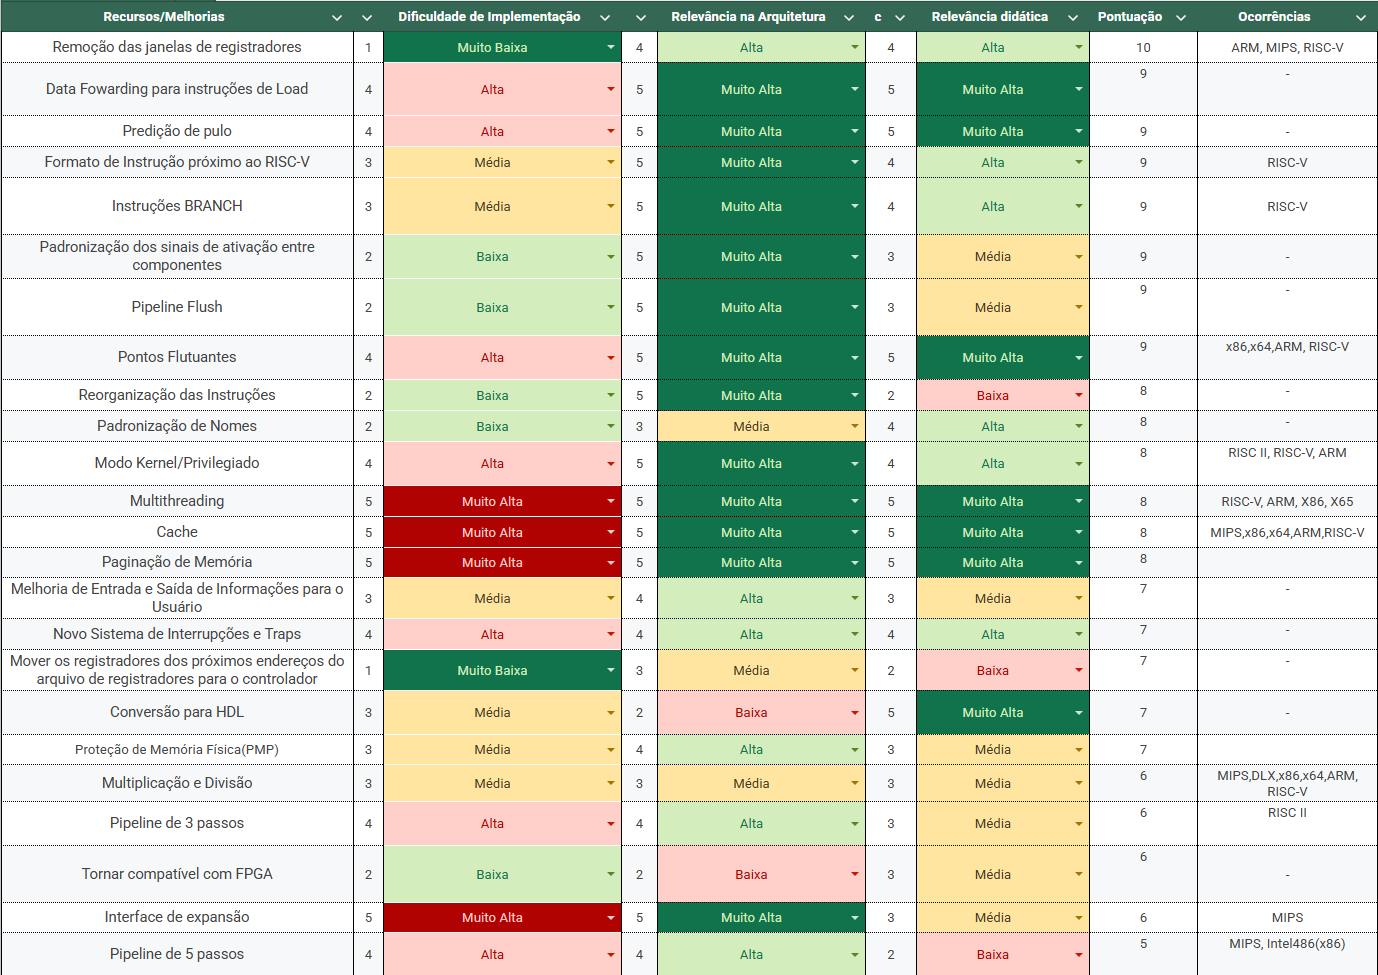
\includegraphics[width=1\linewidth]{RecursosMelhoriasArquitetura.png}
    \caption{Lista de possíveis recursos e melhorias para implementação no \textit{assembler}}
    \label{RecursosMelhoriasArquitetura}
\end{table}

Já a Tabela \ref{RecursosMelhoriasAssembler} é similar a \ref{RecursosMelhoriasArquitetura}, porém é considerada a relevância para o \textit{assembler} no lugar da relevância na arquitetura e as ocorrências listadas são referentes a outras linguagens assembly.

\begin{table}[h]
    \centering
    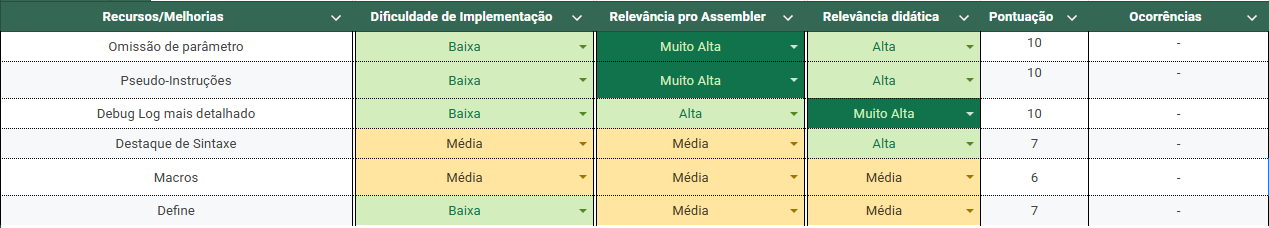
\includegraphics[width=1\linewidth]{RecursosMelhoriasAssembler.png}
    \caption{Lista de possíveis recursos e melhorias para implementação no \textit{assembler}}
    \label{RecursosMelhoriasAssembler}
\end{table}

\subsection{Recursos Para a Arquitetura}
Esta seção apresenta uma descrição de cada recurso da arquitetura na Tabela \ref{RecursosMelhoriasArquitetura}. Recursos que dependem de outros são descritos após suas dependências.

\subsubsection{Remoção das Janelas de Registradores}\label{recursos_remocao}%Não precisa de modificação
As janelas de registradores são um sistema que, em teoria, melhora a performance do processador, além de tornar seu funcionamento mais próximo do \textit{software}. Apesar das aparentes melhorias de desempenho, esse recurso não é encontrado em arquiteturas modernas como ARM \cite{arm_arm_2014}, RISC-V \cite{risc-v_risc-v_2024} ou até mesmo em arquiteturas um pouco mais antigas como MIPS \cite{mips_tech_llc_mips32_2016}.

Isso se deve às suas desvantagens, que incluem a utilização de uma grande porção do circuito, redução da velocidade de \textit{clock} devido aos longos caminhos de barramentos, e o fato de que, em programas que exigem muitas chamadas, ao exceder o número de janelas, as rotinas de salvamento dessas janelas acabam negando os ganhos de performance \cite{patterson_reduced_1985}.

Portanto, a remoção das janelas de registradores seria uma grande otimização para o circuito, além de simplificar a compreensão didática do Arquivo de Registradores.

\subsubsection{Formato de Instrução Próximo ao RISC-V}\label{recursos_risc-v}%Não precisa de modificação
O padrão RISC-V, como mencionado anteriormente na Seção \ref{bibliometry}, tem ganhado popularidade rapidamente, e por ser um padrão aberto, ele se torna uma ótima referência. Além disso, a forma como as instruções são organizadas traz diversas vantagens, que podemos listar:

\begin{itemize}
    \item Posição dos endereços dos registradores consistente entre instruções, simplificando a decodificação \cite{risc-v_risc-v_2024}.
    \item Valores imediatos de algumas instruções alinhados aos \textit{bytes}, facilitando a visualização dentro da instrução.
    \item Redução da quantidade de \textit{opcodes} necessários, em favor da utilização de códigos adicionais que representam diferentes opções por instrução.
    \item A utilização de um padrão amplamente adotado, facilitando a disponibilidade de conteúdo sobre o tema.
    \item O RISC~I, segundo \citeonline{patterson_how_2017}, é possivelmente a arquitetura mais próxima do RISC-V. Em sua comparação, ele cita as seguintes similaridades:
    \vspace{1.5cm}
    \begin{adjustwidth}{4cm}{0cm}
        \fontsize{10pt}{12pt}\selectfont
        \begin{itemize}
            \item Um espaço de endereço endereçável por \textit{bytes} de 32 bits.
            \item Todas as instruções têm 32 bits de comprimento.
            \item 31 registradores, com o registrador 0 fixo em zero, todos com 32 bits de largura.
            \item Todas as operações são registrador-para-registrador (nenhuma é registrador-para-memória).
            \item As mesmas operações aritméticas, lógicas e de deslocamento.
            \item As mesmas instruções de carregar e armazenar \textit{words}.
            \item Versões com e sem sinal de carregar e armazenar \textit{bytes} e \textit{half words} (chamadas de "\textit{short}" no RISC-I).
            \item Opção imediata para todas as instruções aritméticas, lógicas e de deslocamento.
            \item Imediatos são sempre estendidos com sinal.
            \item Um modo de endereçamento de dados (registrador + imediato).
            \item Endereçamento relativo ao contador de programa para saltos.
            \item Sem instruções de multiplicação ou divisão.
            \item Uma instrução para carregar um imediato largo na parte superior do registrador, para que uma constante de 32 bits ocupe apenas duas instruções.
        \end{itemize}
        \citeonline{patterson_how_2017}
    \end{adjustwidth}
    Estas semelhanças facilitam a aplicação do padrão RISC-V ao RISC~I.
\end{itemize}

\subsubsection{Reorganização das Instruções}\label{recursos_reorganizacao}%Não precisa de modificação

A reorganização das instruções pode envolver a alteração dos \textit{opcodes} de cada instrução, com o objetivo de simplificar tanto a decodificação quanto a visualização do conjunto. Uma abordagem eficiente seria adotar a organização utilizada no RISC~II, que apresenta uma ordenação mais direta e uma divisão mais clara entre os diferentes grupos de instruções. Essa melhoria torna-se implícita na implementação do padrão RISC-V, que já incorpora tais princípios de organização.

\subsubsection{Padronização de Nomes}\label{recursos_padronizacao_nome}%Não precisa de modificação

No momento, o circuito criado não possuía um padrão bem definido de nomes, o que dificultava a compreensão da funcionalidade de certas entradas e saídas de alguns componentes. A padronização definiria como esses nomes devem ser escritos para a melhoria da compreensão da função dos componentes e para a melhoria da consistência geral.

\subsubsection{Padronização dos sinais de ativação entre componentes}\label{recursos_padronizacao_sinais}%Não precisa de modificação

A temporização do circuito não está padronizada. Há alguns componentes que se ativam durante a descida do sinal de \textit{clock} enquanto outros se ativam durante a subida. Estes sinais devem ser alterados para melhoria da consistência no funcionamento do circuito e para a prevenção de erros.

\subsubsection{Modo \textit{Kernel}/Privilegiado}\label{recursos_kernel}%Não precisa de modificação
A inclusão de um Modo \textit{Kernel} em uma arquitetura didática é fundamental para ilustrar conceitos essenciais de segurança, controle e organização do sistema. Esse recurso permite demonstrar, de forma clara, como o processador diferencia entre código confiável e não confiável, como ocorrem as transições entre aplicações e o sistema operacional, e como se estabelece o isolamento entre diferentes camadas de software.

Mesmo em ambientes simplificados, compreender os modos de operação ajuda os estudantes a visualizar a estrutura real dos sistemas computacionais modernos e a reconhecer a importância da proteção de recursos e da gestão de privilégios. Além disso, esse conceito reforça a noção de que o sistema operacional atua como uma camada intermediária crítica entre o \textit{hardware} e as aplicações, sendo responsável por garantir o funcionamento seguro e eficiente do sistema.

O Recurso \ref{recursos_risc-v} especifica o funcionamento do modo \textit{kernel}, e poderia ser seguido para esta implementação, resultando em um controle mais padronizado. Esse seria um ótimo recurso para ser ensinado, pois evidencia um dos principais mecanismos de \textit{hardware} para o gerenciamento de um sistema operacional.

\subsubsection{Novo Sistema de Interrupções e \textit{Traps}}\label{recursos_interrupt}%Não precisa de modificação
A implementação de um sistema de \textit{traps} em uma arquitetura didática é essencial para demonstrar como o processador lida com eventos excepcionais e solicitações de serviços do sistema operacional. Esse mecanismo permite que o fluxo de execução seja transferido de forma controlada para rotinas específicas, como chamadas de sistema ou tratamento de erros, garantindo que o sistema possa responder adequadamente a situações inesperadas ou a requisições de alto nível feitas por programas em modo usuário.

Além de reforçar a separação entre os modos de operação, o sistema de \textit{traps} exemplifica como o \textit{hardware} e o sistema operacional colaboram para manter a estabilidade, a segurança e a previsibilidade da execução. Para fins didáticos, esse recurso é valioso por permitir que os estudantes compreendam o papel das interrupções e exceções no funcionamento de sistemas reais, e como essas estruturas são fundamentais para o controle de acesso a recursos privilegiados.

\subsubsection{\textit{Pipeline Flush}}\label{recursos_pipe_flush}%não precisa de modificações

O \textit{pipeline flush} é uma técnica utilizada para limpar a \textit{pipeline} do processador quando ocorre uma mudança no fluxo de controle, como um pulo condicional ou uma interrupção. Quando uma instrução de pulo é executada, as instruções que foram buscadas e decodificadas, mas ainda não executadas, podem não ser mais válidas, pois o fluxo de execução mudou para um novo endereço.

Para evitar a execução de instruções inválidas, o \textit{pipeline flush} limpa todas as instruções que estão atualmente na \textit{pipeline}, garantindo que apenas as instruções do novo fluxo de controle sejam executadas. Isso é feito invalidando as instruções nas etapas da \textit{pipeline} e reiniciando o processo de busca de instruções a partir do novo endereço de destino.

A implementação do \textit{pipeline flush} na arquitetura envolveria a adição de lógica de controle que detecta quando uma mudança no fluxo de controle ocorre e sinaliza para as etapas da \textit{pipeline} que as instruções devem ser invalidadas. Essa técnica é essencial para manter a integridade do fluxo de execução e evitar erros causados pela execução de instruções incorretas.

\subsubsection{Melhoria na Entrada e Saída de Informações para o Usuário}\label{recursos_melhoria_IO}%não precisa de modificações

Durante a replicação do RISC~I, foram exploradas algumas formas rudimentares de interface de entrada e saída. No entanto, é desejável desenvolver mecanismos mais eficientes de interação com o sistema, tanto para fins didáticos, demonstrando o funcionamento dos dispositivos de entrada, quanto para aplicações práticas.

Para entrada de dados pelo usuário, podem ser utilizados dispositivos como teclado, \textit{joystick} e \textit{sliders}. Já para saída, opções incluem um terminal e uma tela gráfica simples.

\subsubsection{Mover os registradores dos próximos endereços do Arquivo de Registradores para o controlador}\label{recursos_mover_reg_regfile}%não precisa de modificações

Esta mudança tem como foco a exclusão dos registradores de endereço localizados dentro do Arquivo de Registradores. Com a adoção do padrão RISC-V, esses registradores já seriam modificados a favor das diferenças no funcionamento de determinadas instruções. No entanto, a principal motivação foi a simplificação da forma como as instruções em execução são armazenadas no controlador.

Em vez de distribuir uma instrução por diferentes partes do processador, é possível concentrar todas as informações em um único controlador. Essa abordagem facilita o gerenciamento e a visualização das instruções em execução, além de centralizar os sinais de controle de maneira mais eficiente.

\subsubsection{Multiplicação e Divisão}\label{recursos_muldiv}%não precisa de modificações

Multiplicação e divisão são operações que geralmente não são abordadas em arquiteturas didáticas. A adição dessas operações pode oferecer uma perspectiva sobre o funcionamento delas dentro de uma arquitetura. O RISC-V possui uma extensão, denominada M, que implementa ambas as operações e pode ser seguida para a implementação. No entanto, caso a divisão se revele difícil para implementação, é possível adicionar apenas as operações de multiplicação, que no RISC-V estão dentro do sub-conjunto da extensão M, denominado Zmmul.

\subsubsection{Pontos Flutuantes}\label{recursos_float}%não precisa de modificações, 

Similar a multiplicação e divisão, operações com pontos flutuantes deveriam ser abordadas dentro de arquiteturas didáticas. Estas operações são definidas em diversas extensões do RISC-V, porém o foco principal seria a extensão F, que define os operações com precisão única(32 bit), descrita pelo padrão IEEE 754-2008\cite{risc-v_risc-v_2024}. As extensões que definem outros tamanhos de ponto flutuantes podem ser consideradas para implementações futuras, porém a implementação mínima apenas requer precisão única.

\subsubsection{\textit{Pipeline} de 3 passos}\label{recursos_pipe3}%não precisa de modificações,

O RISC~I possui uma \textit{pipeline} de 2 passos, onde o primeiro é a coleta da instrução e decodificação enquanto a segunda é a execução. Esta \textit{pipeline} pode ser otimizada ao adicionar um terceiro passo, que executa o segundo ciclo de execução de instruções de \texttt{load} e \texttt{store} em paralelo com os outros ciclos.

Este tipo de \textit{pipeline} foi executada no RISC~II, e melhora execução destas instruções, porém ela pode introduzir dependência de dados que devem ser tratadas por software ou hardware.

\subsubsection{Encaminhamento de dados para Instruções de \texttt{load}}\label{recursos_forward}%não precisa de modificações,

\textit{Data forwarding} ou Encaminhamento de dados  é uma técnica utilizada para resolver dependências de dados em pipelines via hardware, especialmente em instruções de \texttt{load}. No caso da \textit{Pipeline} de 3 passos mencionada anteriormente, as instruções de \texttt{load} demoram um ciclo adicional para a gravação do dado no registrador, o que causa a instrução que vem a seguir utilizar o antigo valor desse registrador.

Ao encaminhar dados diretamente das etapas de carregamento para as etapas de execução de instruções subsequentes, podemos evitar atrasos causados por acessos à memória, melhorando a eficiência geral do \textit{Pipeline} e evitando problemas. Caso este recurso seja difícil para implementação, um aviso deve ser adicionado no \textit{assembler}, indicando quaisquer conflitos de dados.

\subsubsection{\textit{Pipeline} de 5 passos}\label{recursos_pipe5}%não precisa de modificações,

Uma \textit{pipeline} de 5 passos é uma evolução da \textit{pipeline} de 3 passos, adicionando mais estágios para aumentar o paralelismo e, consequentemente, o desempenho do processador. Os cinco estágios típicos são:
\begin{itemize}
    \item \textbf{Busca de Instrução (IF):} Localiza e carrega a próxima instrução da memória.
    \item \textbf{Decodificação (ID):} Interpreta a instrução e identifica os operandos necessários.
    \item \textbf{Execução (EX):} Realiza a operação indicada pela instrução.
    \item \textbf{Acesso à Memória (MEM):} Lê ou escreve dados na memória, quando necessário.
    \item \textbf{Escrita de Resultado (WB):} Armazena o resultado da operação nos registradores.
\end{itemize}

Esse tipo de \textit{pipeline} é implementado em arquiteturas como a MIPS\cite{mips_tech_llc_mips32_2016} e fornece uma melhoria na performance. No entanto, pode aumentar a complexidade do circuito, o que pode dificultar o entendimento didático do funcionamento da \textit{pipeline}. Caso seja implementada, esse aspecto deve ser considerado.

Vale destacar que os estágios de busca de instrução e acesso à memória podem gerar conflitos quando executados simultaneamente, já que ambos requerem acesso à memória principal. Para evitar esse problema, é necessário empregar técnicas que permitam o acesso paralelo ou escalonado à memória, garantindo o funcionamento correto da \textit{pipeline}.

\subsubsection{Instruções \textit{branch}}\label{recursos_branch}%não precisa de modificações,

As instruções de pulo condicional do RISC~I exigem que primeiro uma operação seja executada como subtração ou soma para que códigos de condição sejam definidos. Esses códigos são então testados utilizando uma condição selecionada na instrução do pulo.

Este processo pode ser simplificado por um tipo de operação chamada de \textit{branch}, que executa uma subtração seguida dos testes de condição, tudo dentro de um ciclo da mesma instrução, tornando o processo bem mais direto. Este tipo de pulo condicional é definido no conjunto de instrução base do RISC-V junto com instruções para pulos não condicionais.

\subsubsection{Predição de pulo}\label{recursos_pred_pulo}%não precisa de modificações

Predições de pulo, assim como o \textit{data forwarding}, são formas de otimizar a \textit{pipeline} e evitar \textit{hazards} na arquitetura. Na predição de pulo, durante a fase de coleta da próxima instrução, se a instrução atual for um pulo, a instrução a ser coletada deve ser a do endereço definido pelo pulo.

Esse processo pode ser simples para pulos não condicionais, pois eles sempre são executados. No entanto, para instruções de pulos condicionais, esse processo é mais complexo, pois só é possível saber se o pulo será tomado após a verificação da condição, que geralmente ocorre ao fim do ciclo, deixando pouco ou nenhum tempo para obter dados do endereço do pulo.

Uma possível solução é coletar a instrução tanto do endereço seguinte ao pulo quanto do endereço definido pelo pulo. No entanto, isso pode exigir um aumento na quantidade de passos por ciclo da \textit{pipeline}, reduzindo a performance geral.

O mecanismo de predição de pulo possui uma alta relevância didática, pois mostra uma das possíveis otimizações que são implementadas em \textit{pipelines}. Caso implementada, a predição de pulo torna o recurso de \textit{pipeline flush}(\ref{recursos_pipe_flush}) obsoleto.

\subsubsection{Conversão para HDL}\label{recursos_hdl}%não precisa de modificações

A conversão da arquitetura para linguagens de descrição de hardware como SystemVerilog ou VHDL permite a implementação e simulação em nível de hardware de forma mais eficiente que a simulação em simuladores com interface gráfica como o Logisim.

Isso é essencial para validar a funcionalidade e desempenho da arquitetura de forma automatizada, bem como para realizar síntese e implementação em FPGA o que exige a descrição por essas linguagens.

\subsubsection{Tornar compatível com FPGA}\label{recursos_fpga}%não precisa de modificações

Tornar a arquitetura compatível com FPGA envolve não só a descrição por linguagens HDL, mas também uma adaptação do design para que possa ser sintetizado e implementado em dispositivos FPGA. Isso inclui a otimização do uso de recursos de hardware disponíveis no FPGA, remoção de componentes que não são compatíveis com FPGAs e a verificação da funcionalidade por meio de simulações e testes no hardware.

Uma interface física também deve ser implementada para que o usuário possa interagir com o processador, o que pode requerer a implementação de protocolos de comunicação de dispositivos de entrada e saída como I²C, SPI, UART ou USB.

A realização desse passo agrega valor ao projeto por diversos motivos. Primeiramente, permite a validação prática da arquitetura em um ambiente físico, essencial para verificar o funcionamento real do sistema além da simulação, fortalecendo a confiabilidade dos resultados obtidos.

Além disso, a implementação em FPGA possibilita a interação direta com periféricos reais, ampliando o escopo do projeto e permitindo demonstrar aplicações concretas. Essa etapa também evidencia o domínio de ferramentas e práticas utilizadas na indústria de sistemas digitais, tornando o projeto mais robusto e relevante tanto em contextos acadêmicos quanto profissionais.

\subsubsection{Interface de Expansão}\label{recursos_expan}%não precisa de modificações,

Uma interface de expansão permitiria a adição modular de componentes ao processador, como co-processadores (por exemplo, FPUs, TPUs ou GPUs). Essa interface é essencial para aumentar a flexibilidade e a capacidade de processamento do sistema, diferindo da interface com dispositivos de entrada e saída, pois é projetada para comunicação direta e de alta velocidade entre o processador principal e os módulos de expansão.

Para implementar a interface de expansão, é necessário definir um protocolo de comunicação eficiente entre o processador e os módulos de expansão. Esse protocolo deve incluir a definição de comandos específicos para inicialização, leitura e escrita de dados, interrupções e os sinais e barramentos que serão compartilhados entre o processador e os dispositivos de expansão.

\subsubsection{\textit{Multithreading}}\label{recursos_multithreading}%

Do ponto de vista educacional, a implementação de multithreading em uma arquitetura de processador oferece uma oportunidade para explorar conceitos fundamentais de concorrência, paralelismo e gerenciamento de contexto. Ao lidar com múltiplos fluxos de execução, o estudante é exposto a desafios reais enfrentados em arquiteturas modernas, como escalonamento de tarefas, sincronização e compartilhamento de recursos.

Do ponto de vista arquitetural, implementar multithreading exige a criação de mecanismos para gerenciamento de contexto, como registradores duplicados, controle de escalonamento e sincronização entre threads. Embora isso aumente a complexidade do design, também proporciona uma oportunidade valiosa de explorar conceitos avançados de arquitetura de processadores.

A inclusão de multithreading agrega valor ao projeto por permitir a análise de desempenho em cenários reais, além de demonstrar a escalabilidade da arquitetura. Academicamente, essa funcionalidade evidencia o domínio de técnicas modernas de projeto de sistemas computacionais e aproxima o trabalho das práticas adotadas em processadores comerciais.

\subsubsection{Memória \textit{Cache}}\label{recursos_cache}%não precisa de modificações,

A memória \textit{cache} é um recurso presente na maioria dos sistemas computacionais modernos, sendo essencial para aumentar a eficiência de acesso à memória principal pelo processador.

Além de acelerar a leitura e escrita de dados, a separação entre dados e instruções proporcionada pelo \textit{cache} L1 viabiliza a implementação de uma pipeline de cinco estágios, ao eliminar conflitos de acesso à memória durante a busca de instruções e operações com dados.

\subsubsection{Paginação de Memória}\label{recursos_mem_pag}%mover uma porção daqui para a fundamentação teórica

Para implementar a paginação de memória no \textit{hardware}, é necessário incluir uma Unidade de Gerenciamento de Memória (MMU). A MMU é responsável por traduzir endereços virtuais em endereços físicos. Os passos que estariam envolvidos nesse processo são:

\begin{enumerate}
    \item \textbf{Adicionar uma MMU}: Esse componente ficaria entre o processador e a memória. Ele traduz os endereços virtuais gerados pelos programas em endereços físicos na memória RAM.    
    \item \textbf{Configurar Tabelas de Páginas}: Tabelas de páginas seriam criadas para mapear os endereços virtuais para os endereços físicos. Cada entrada na tabela de páginas contém o endereço físico correspondente e permissões de acesso.    
    \item \textbf{Gerenciar Falhas de Página}: Um mecanismo para lidar com falhas de página teria que ser implementado. Quando uma página solicitada não estiver na memória física, a MMU deve sinalizar uma falha de página, e o sistema operacional deve carregar a página do disco rígido para a memória.    
    \item \textbf{Permissões e Proteção}: As permissões de acesso na tabela de páginas devem ser configuradas para garantir que cada processo tenha acesso apenas às suas próprias páginas, evitando erros.
\end{enumerate}

Esse recurso seria relativamente complexo e depende de vários outros como o modo \textit{kernel} e \textit{cache}, porem devido à sua importância, é um ótimo recurso a ser considerado caso haja tempo para a sua implementação.

\subsection{Recursos Para a Assembler}
\subsubsection{Omissão de parâmetro}\label{recursos_omissao}
A omissão de parâmetro é um recurso que facilita a criação de código assembly, permitindo que o programador não precise preencher parâmetros que não são usados pela instrução. Isso simplifica a escrita do código, tornando-o mais legível e menos propenso a erros. Por exemplo, em uma instrução que não utiliza um segundo operando, o programador pode omitir esse parâmetro, e o \textit{assembler} tratará a ausência de forma adequada, utilizando um valor padrão ou ignorando o parâmetro omitido.

\subsubsection{Pseudo-Instruções}\label{recursos_pseudo_inst}%feito
Para auxiliar na programação do código assembly, pseudo-instruções podem ser criadas. Esse é um recurso presente em diversas linguagens assembly que traz a possibilidade de emular instruções não existentes na arquitetura a partir de outras.

Diversos exemplos de pseudo-instruções são mostrados no manual do RISC-V \cite{risc-v_risc-v_2024}, como a instrução de negação (NOT), que pode ser sintetizada por um ou exclusivo (XOR), ou instruções de desvio condicional (BLT, BGE), que podem ser invertidas ao alterar a ordem dos operandos (BGT, BLE).

Para que seja possível a implementação de pseudo-instruções, uma reestruturação do \textit{assembler} pode ser necessária. Esse recurso pode também completar a omissão de parâmetros, uma vez que pseudo-instruções podem ser definidas com diferentes quantidades de parâmetros necessários.

\subsubsection{\textit{Debug Log} mais detalhado}\label{recursos_debug_log}
\begin{figure}[h]
\centering
\begin{lstlisting}
Current line: AND R1 R1 #FFFFFC7F

10000000000000000000000000000000 Instruction AND(2164260864) added to [27] with:
00000000000010000000000000000000 Destination: 00080000
00000000000000000100000000000000 Source 1: 00004000
00000000000000000001110001111111 Immediate: 00001c7f
\end{lstlisting}
\caption{Exemplo da impressão de uma instrução realizada pelo \textit{assembler}}
\label{fig:assemblerRuim}
\end{figure}

Durante a primeira versão do \textit{assembler}, informações sobre a montagem do código eram exibidas. No entanto, essas informações não eram intuitivas e eram incompletas, conforme pode ser observado na Figura~\ref{fig:assemblerRuim}.

O \textit{assembler} deveria fornecer informações mais diretas e apresentar mensagens de erro claras. Algumas melhorias que poderiam ser implementadas incluem:
\begin{itemize}
  \item Impressão de uma linha por tradução, que deve exibir o resultado da tradução e comparação com o código original.
  \item Uma melhor detecção de erros sintáticos.
  \item Adição de detecção de erros semânticos, que incluiria avisos ao utilizar recursos não inicializados ou acesso a endereços inválidos.
  \item Impressão dos passos de criação e tradução de rótulos e variáveis.
  \item Detecção de \textit{hazards} na pipeline
\end{itemize}

\subsubsection{Destaque de Sintaxe}\label{recursos_syntax}
O destaque de sintaxe é uma funcionalidade que melhora a legibilidade e a compreensão do código-fonte ao aplicar diferentes cores e estilos de formatação a elementos distintos da linguagem de programação. Isso inclui palavras-chave, variáveis, strings, comentários e outros componentes sintáticos.

A principal vantagem do destaque de sintaxe é facilitar a identificação de diferentes partes do código, tornando mais fácil detectar erros e entender a estrutura e a lógica do programa. Além disso, o destaque de sintaxe pode acelerar o processo de escrita de código, pois ajuda os programadores a reconhecer rapidamente os elementos da linguagem e a evitar erros comuns.

Implementar o destaque de sintaxe em qualquer IDE que possa ser utilizada para programar o código assembly pode melhorar significativamente a experiência do usuário, tornando a escrita e a leitura do código assembly mais intuitivas e eficientes. Isso é especialmente útil em ambientes educacionais, onde a clareza e a facilidade de uso são essenciais para o aprendizado.

\subsubsection{Macros}\label{recursos_macro}
Macros são uma ferramenta em linguagens de montagem que permitem a definição de sequências de instruções que podem ser reutilizadas em diferentes partes do código. Elas funcionam como uma espécie de função ou procedimento, onde um conjunto de instruções é agrupado sob um nome específico. Quando esse nome é chamado no código, o conjunto de instruções associado é inserido no lugar.

As macros ajudam a reduzir a repetição de código, facilitam a manutenção e melhoram a legibilidade do código assembly. Elas são especialmente úteis para operações complexas ou frequentemente repetidas, permitindo que o programador defina a sequência de instruções uma vez e a reutilize conforme necessário.

A implementação de macros no \textit{assembler} envolve a criação de um pré-processador que expande as macros antes da montagem do código. Isso significa que, durante a fase de pré-processamento, o \textit{assembler} substitui todas as chamadas de macros pelas instruções definidas na macro, gerando o código final que será montado.

\subsubsection{Define}\label{recursos_define}

O recurso \textit{define} é uma funcionalidade encontrada em \textit{assembly} e outras linguagens de programação que permite a definição de constantes ou macros. Em um \textit{assembler}, o \textit{define} é usado para atribuir um nome a um valor constante ou a uma sequência de instruções, facilitando a leitura e a manutenção do código.

Por exemplo, em um \textit{assembler}, você pode definir uma constante para um endereço de memória específico:

\begin{lstlisting}
#define START_ADDRESS 0x1000
\end{lstlisting}

Isso permite que você use \textit{START\_ADDRESS} em vez de 0x1000 em todo o seu código, tornando-o mais legível e fácil de modificar. Se o endereço precisar ser alterado, você só precisará atualizar a definição, em vez de procurar e substituir todas as ocorrências do valor no código.

O uso de \textit{define} melhora a clareza e a manutenção do código, permitindo a criação de nomes significativos para valores constantes.

\section{Implementação dos Recursos e Melhorias}

Apesar do planejamento na metodologia indicar a implementação de cada recurso em ciclos separados, pelo tipo de relação entre alguns desses recursos, parte das implementações ocorreu em paralelo. Nesta seção será descrito em ordem de implementação todos os recursos que foram adicionados. Caso um recurso descrito em \ref{recursosMelhorias} seja citado, a seção que o descreve será exibida entre parênteses, como exemplo o cache(\ref{recursos_cache});

\subsection{Processo de Desenvolvimento - Arquitetura}

\subsubsection{Primeira Fase: Alterações Iniciais}

As primeiras melhorias focaram em tornar o sistema compatível com o conjunto de instruções RISC-V (\ref{recursos_risc-v}), começando pelo \textit{assembler} descrito na Seção \ref{process_assembler}. Após as adaptações realizadas no \textit{assembler}, a primeira melhoria implementada foi a remoção das janelas de registradores (\ref{recursos_remocao}), que simplificou significativamente o circuito necessário e eliminou a necessidade de rotinas de tratamento de interrupções relacionadas ao \textit{overflow} do número de janelas. Isso também economizou tempo ao remover a necessidade de adaptar esses recursos para o novo conjunto de instruções.

Para a remoção das janelas de registradores, três componentes precisaram ser modificados: o Arquivo de Registradores, a Palavra de Status do Processador e o Controlador - enquanto o Controlador do Número de Janela foi removido totalmente.

O Arquivo de Registradores sofreu a maior modificação, que envolveu a remoção do controle relacionado às janelas, deixando apenas uma versão expandida dos registradores globais, renomeada como \textit{Registers Bank} (Banco de Registradores). Adicionalmente, os registradores de endereço foram movidos para o controlador (\ref{recursos_mover_reg_regfile}), aproveitando que ambos os componentes já estavam sendo modificados.

\begin{figure}[ht]
    \centering
    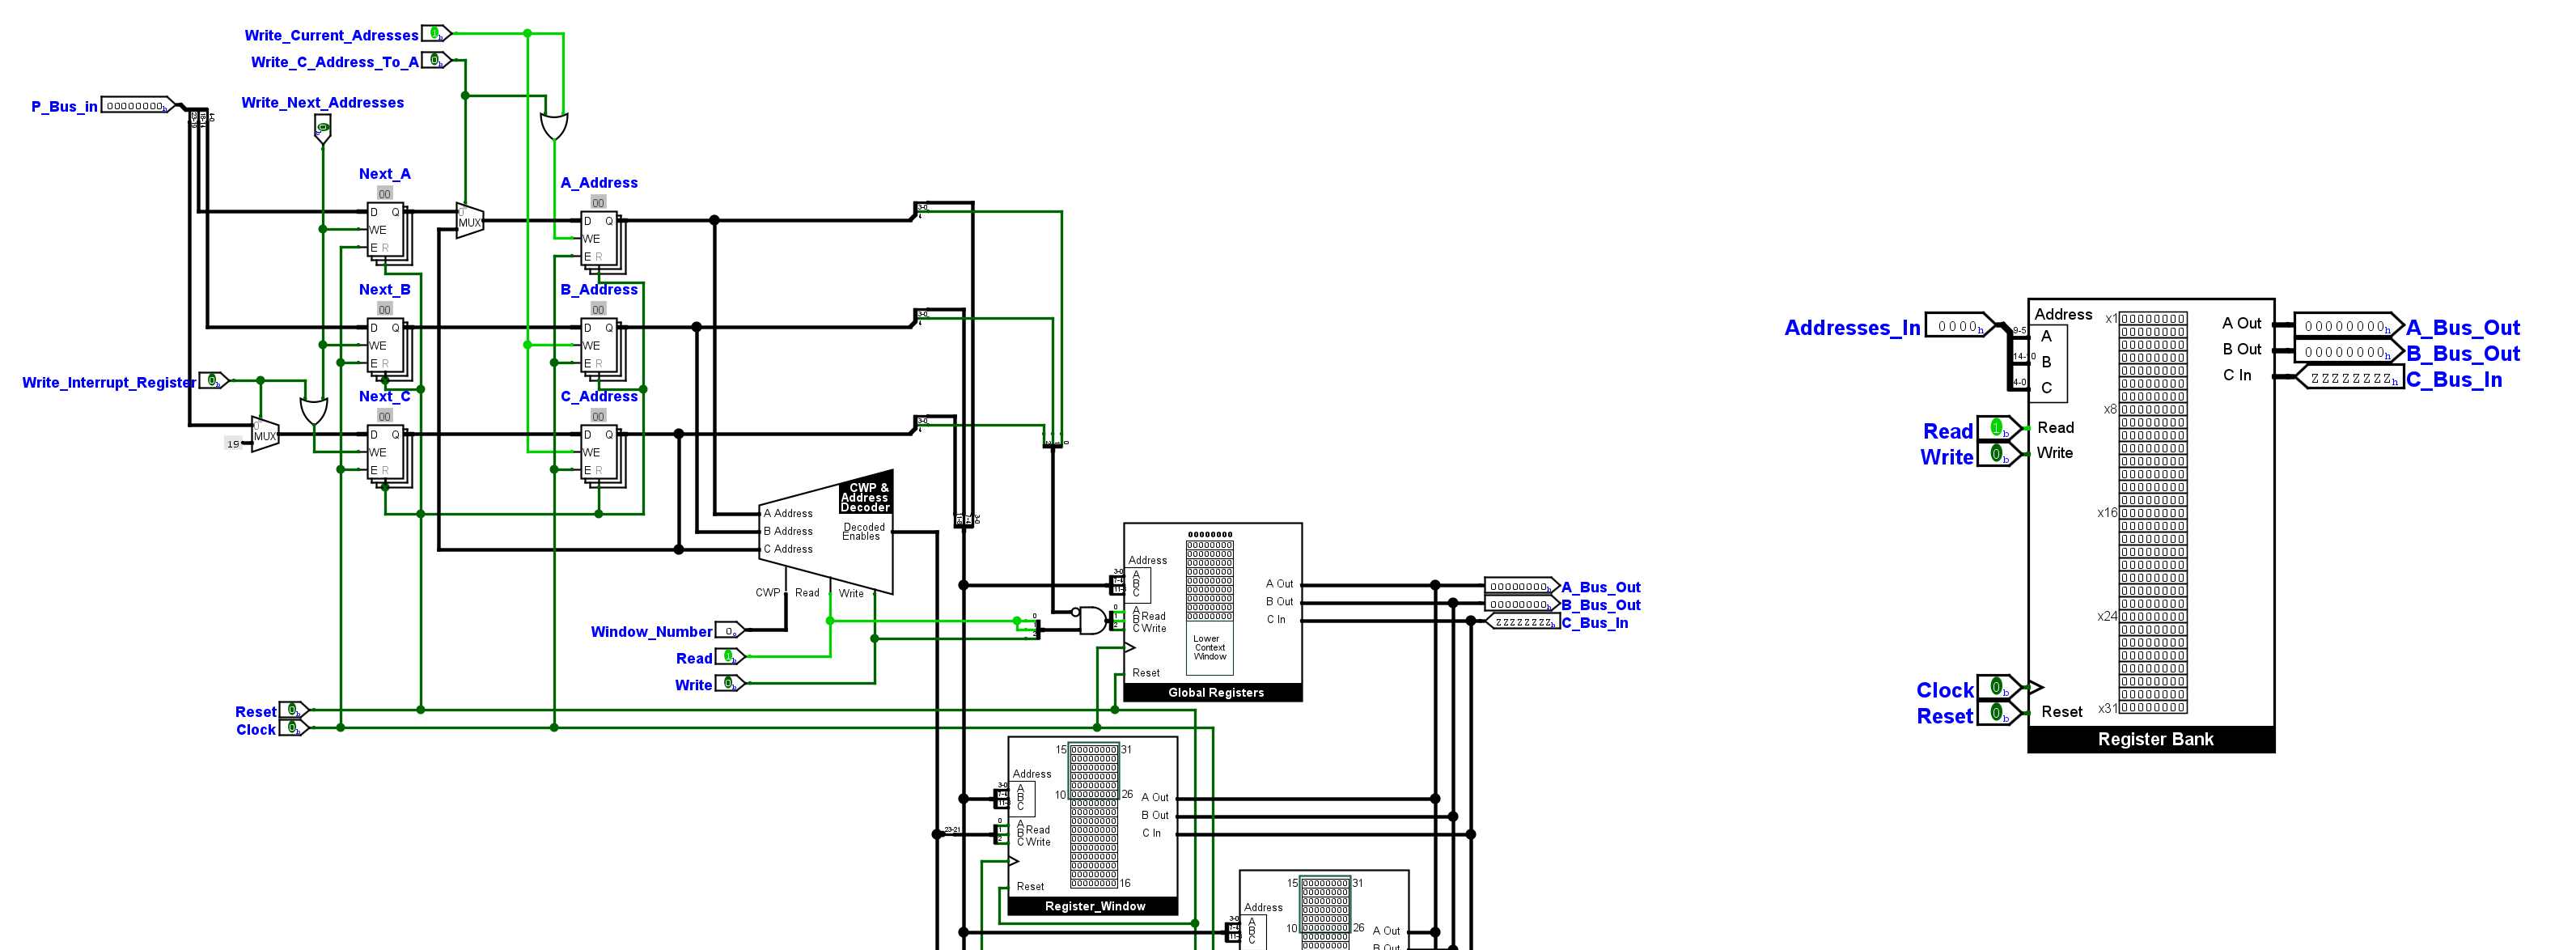
\includegraphics[width=1\linewidth]{ProcessoDesenvolvimento/Arquitetura/RegisterFile.png}
    \caption{Arquivo de Registradores antes (esquerda) e depois (direita) da modificação.}
    \label{fig:desenvolvimento_register_file}
\end{figure}

A Figura~\ref{fig:desenvolvimento_register_file} mostra o resultado das modificações realizadas no Arquivo de Registradores. É possível notar que, neste ponto, o Banco de Registradores possui as mesmas entradas e saídas que o Arquivo de Registradores, o que o torna apenas um encapsulador. Isso foi feito considerando que o Arquivo de Registradores poderia ser expandido em alguma etapa seguinte para suportar pontos flutuantes, criando a necessidade de outro Banco de Registradores dentro do Arquivo de Registradores.

\begin{figure}[h]
    \centering
    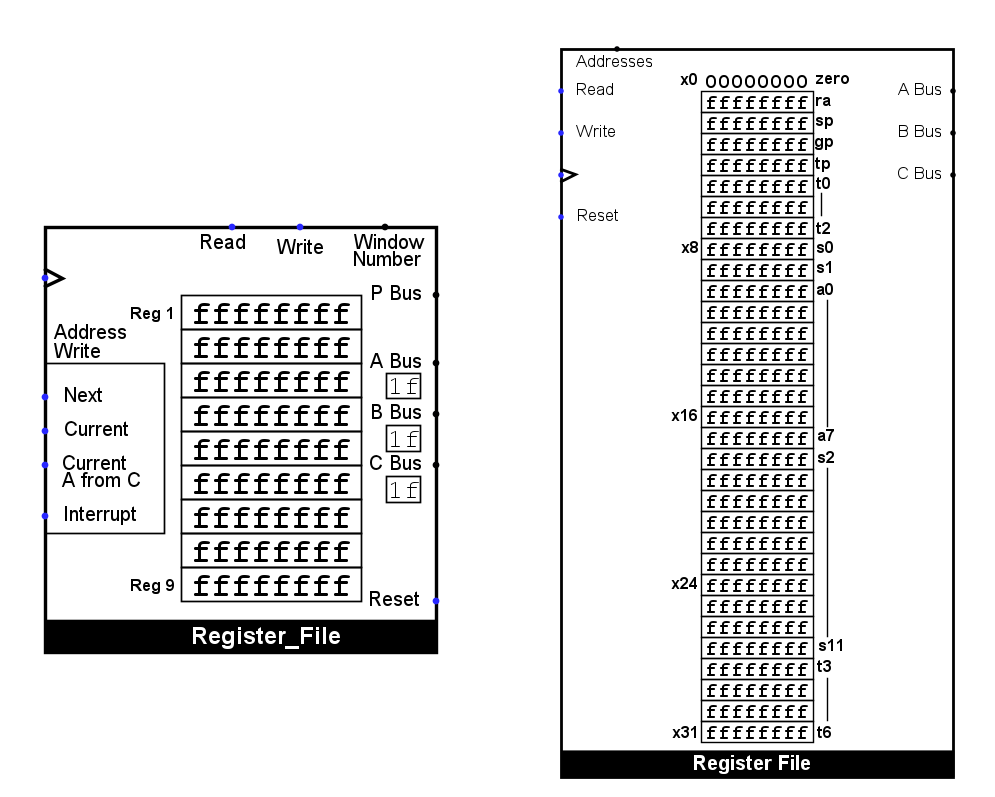
\includegraphics[width=0.5\linewidth]{ProcessoDesenvolvimento/Arquitetura/RegisterFileComponent.png}
    \caption{Encapsulamento do Arquivo de Registradores antes (esquerda) e depois (direita) da modificação.}
    \label{fig:desenvolvimento_register_file_component}
\end{figure}

A Figura~\ref{fig:desenvolvimento_register_file_component} mostra as alterações feitas no encapsulamento do componente. A remoção das janelas permitiu que todos os registradores do arquivo fossem mostrados. Foram atribuídos nomes aos registradores que indicam o uso recomendado, seguindo a especificação do \citeonline{risc-v_risc-v_2024}. Com todas as modificações, a interface do Arquivo de Registradores também foi simplificada, facilitando o controle necessário para utilizá-lo.

A Palavra de Status do Processador (PSW) no RISC-I servia apenas a duas funções: armazenar um espelhamento dos números de janela e o código CNZV (\textit{carry}, negativo, zero e \textit{overflow}) resultante da ALU. Com a remoção do Controlador do Número de Janela, parte da função do PSW foi eliminada, e como as instruções do RISC-V não necessitam do armazenamento dos códigos CNZV, a PSW tornou-se um componente desnecessário para o sistema, permitindo sua remoção.

Para adaptar o Controlador às novas modificações, seus registradores de instrução foram alterados, e a decodificação e transmissão de sinais para controle do número de janela e do PSW foram removidas. Em paralelo, o conjunto de instruções do RISC-V (\ref{recursos_risc-v}, consequentemente \ref{recursos_reorganizacao}) estava sendo adicionado ao modelo. Ao adaptar o conjunto de instruções do RISC-I para o RISC-V, notou-se que o circuito necessário para o controle tornou-se bem mais simples, como pode ser visto nas Figuras \ref{fig:Controlador_1_1} e \ref{fig:Controlador_1_2}.

\begin{figure}[h]
    \centering
    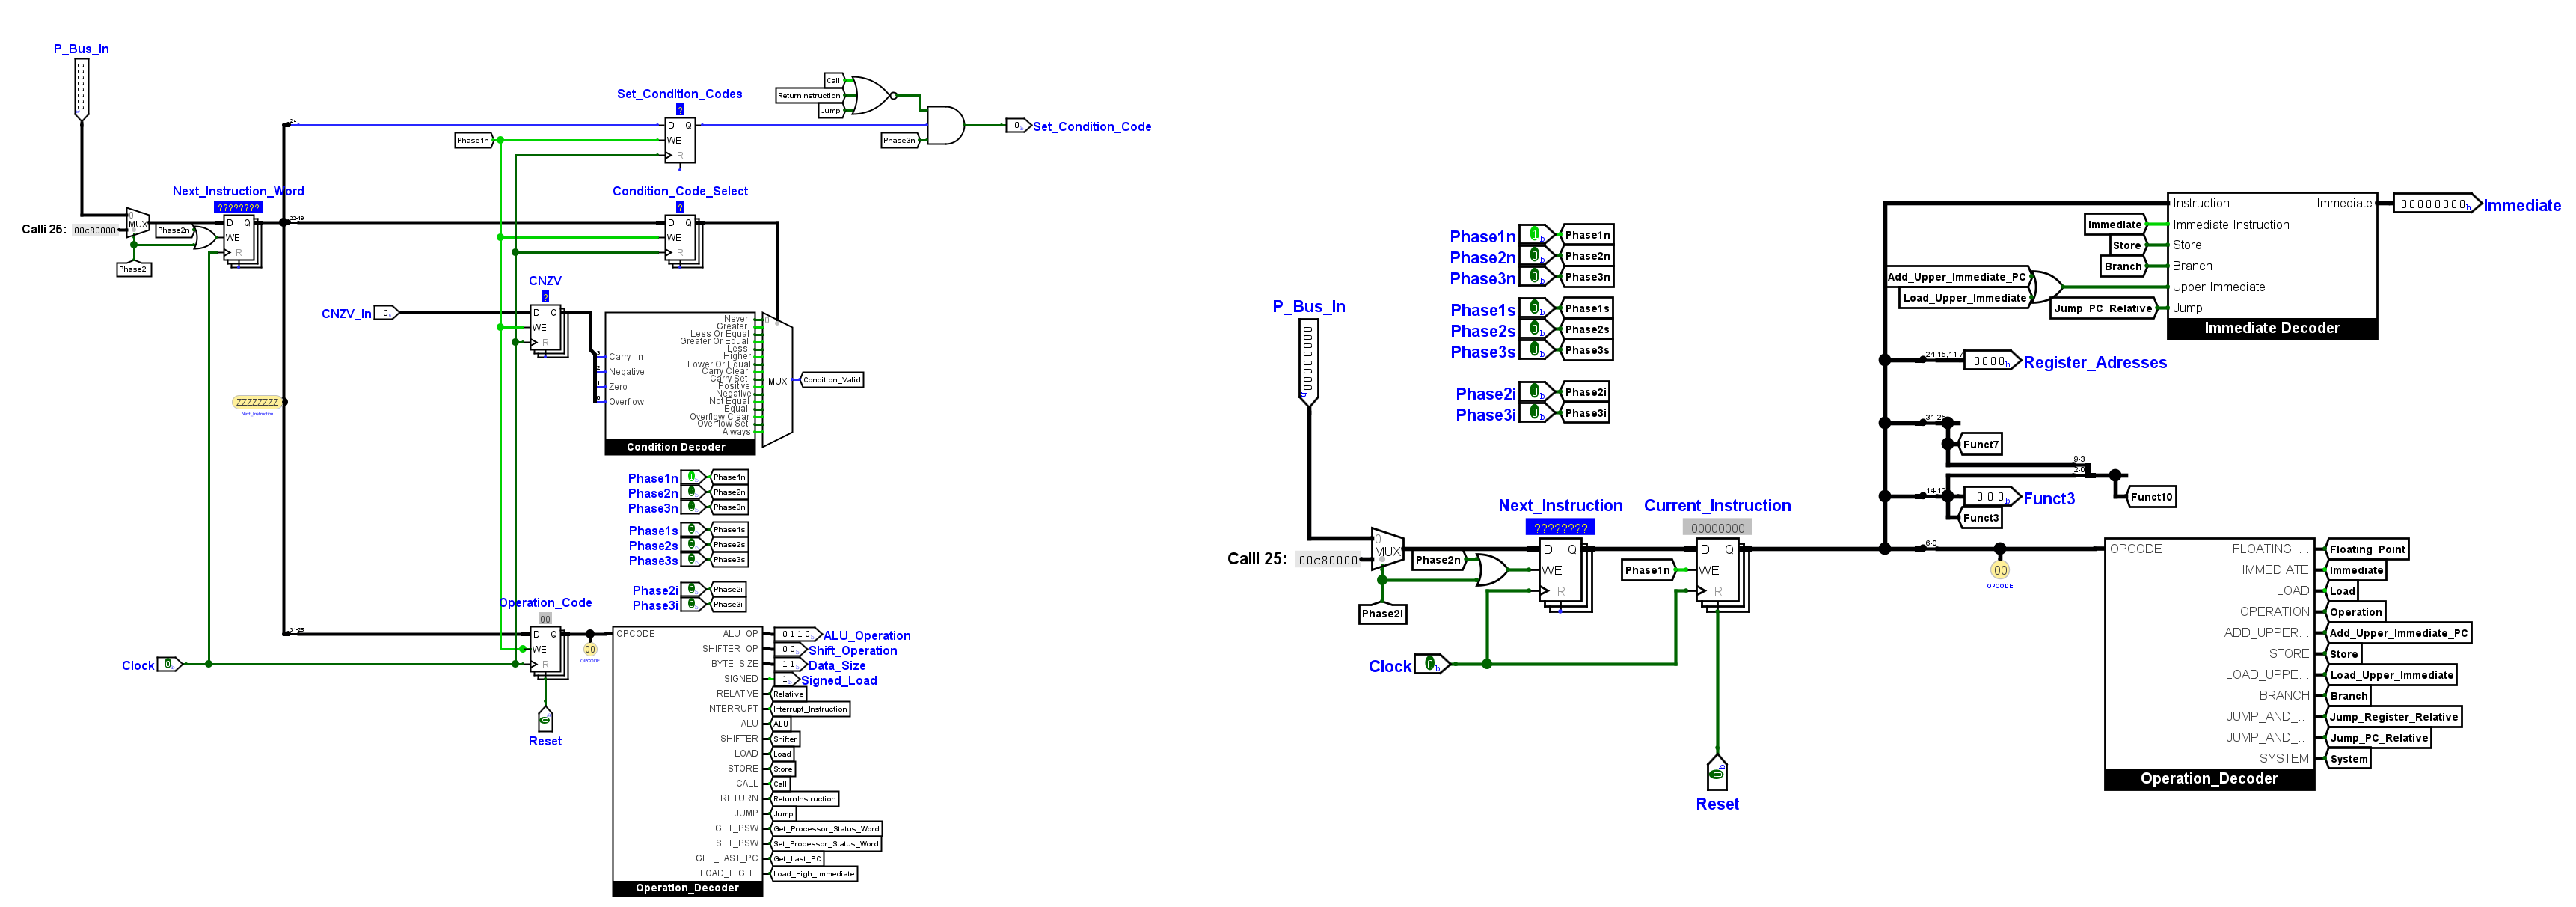
\includegraphics[width=1\linewidth]{ProcessoDesenvolvimento/Arquitetura/Controlador_1_1.png}
    \caption{Primeira fase de decodificação de instruções. Antes (esquerda) e depois (direita).}
    \label{fig:Controlador_1_1}
\end{figure}

\begin{figure}[h]
    \centering
    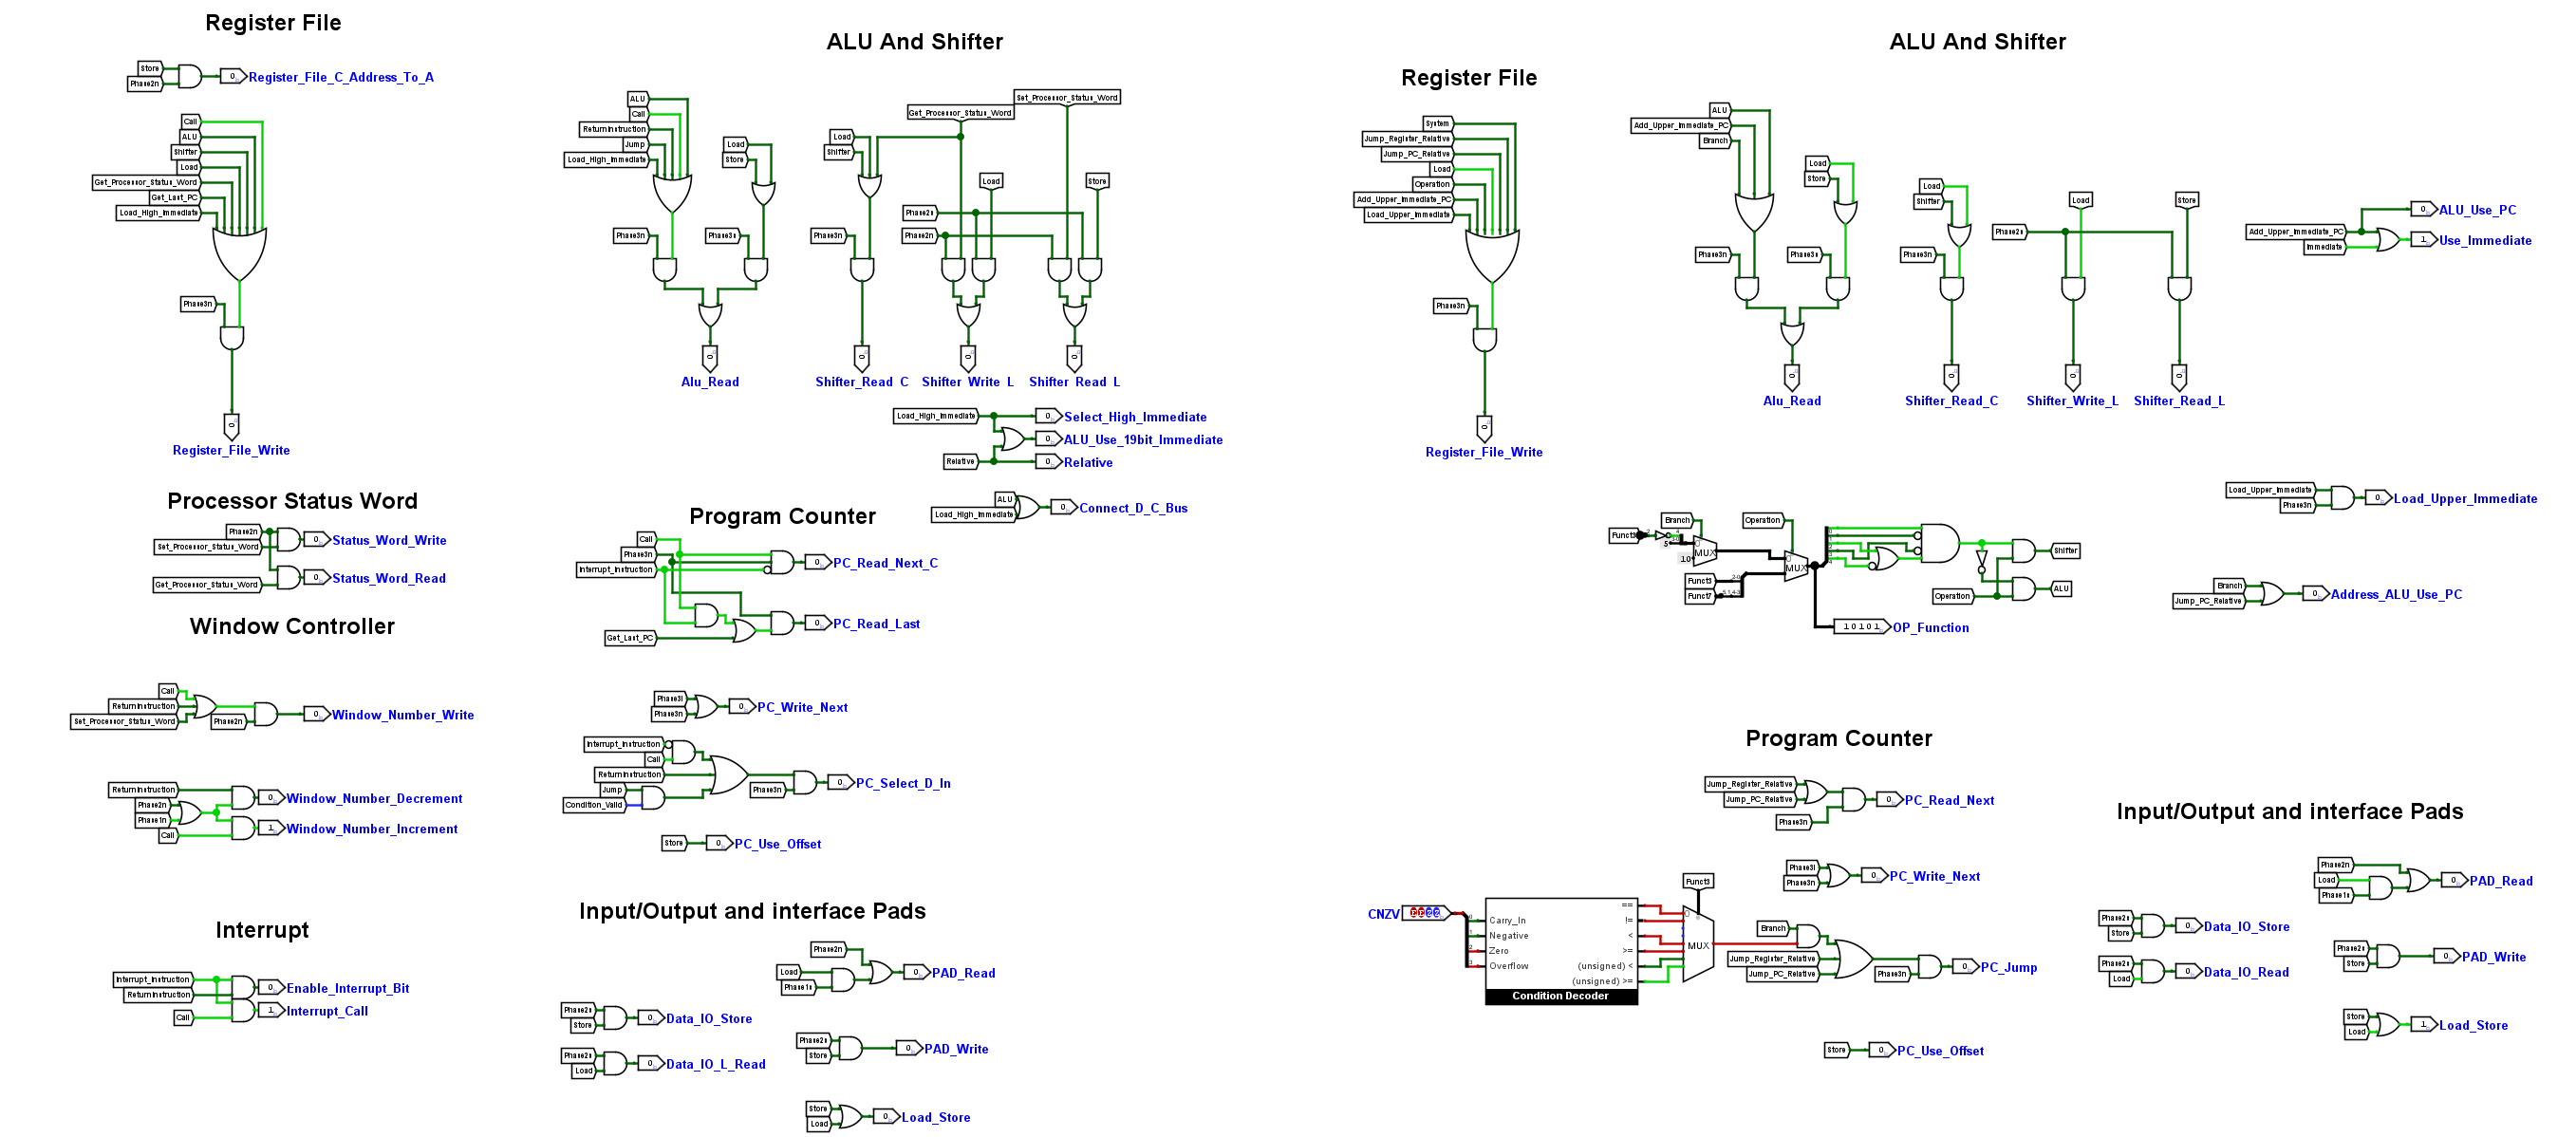
\includegraphics[width=1\linewidth]{ProcessoDesenvolvimento/Arquitetura/Controlador_1_2.png}
    \caption{Segunda fase de decodificação de instruções. Antes (esquerda) e depois (direita).}
    \label{fig:Controlador_1_2}
\end{figure}

Essa simplificação se deve a alguns fatores. O primeiro fator é que o conjunto de instruções base do RISC-V possui uma quantidade menor de instruções em comparação com o RISC-I, o que simplifica o decodificador de instruções. Apesar de possuir menos instruções, as capacidades desse conjunto são equivalentes às do RISC-I, pois cada instrução pode possuir mais funções, que são definidas por códigos dentro da palavra da instrução, o que nos leva ao segundo fator.

Os códigos de função, por estarem separados do \textit{opcode}, podem ser passados diretamente para os componentes do processador, com o mínimo de decodificação necessário. Esses códigos são sempre definidos nas mesmas posições, facilitando o processo de extração. Isso pode ser visto na Figura~\ref{fig:risc-v_op_format}, que mostra a posição do \textit{funct3} e do \textit{funct7}.

\begin{figure}[h]
    \centering
    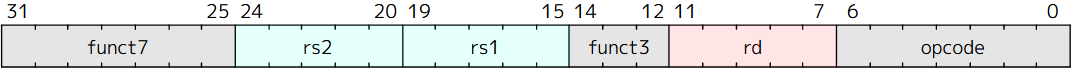
\includegraphics[width=1\linewidth]{ProcessoDesenvolvimento/Arquitetura/risc-v_op_format.png}
    \caption{Formato de instrução do RISC-V para operações entre registradores \cite{risc-v_risc-v_2024}}
    \label{fig:risc-v_op_format}
\end{figure}

Nem todas as instruções e componentes necessitam do \textit{funct7} para funcionar, por isso há uma separação. Exemplos do que esses códigos podem representar são: operações lógico-aritméticas (adição, subtração, \textit{or}, \textit{and}, deslocamento de bits, etc.), tamanho e sinalização de um valor (\textit{byte}, \textit{short}, \textit{word}, com ou sem sinal) e condições (maior que, igual, diferente, etc.).

Outra alteração necessária para tornar o sistema compatível com o RISC-V é a forma como os valores imediatos são salvos e tratados. No RISC-I, há um componente exclusivo para o armazenamento e decodificação do valor imediato. Na nova versão, o registrador da instrução atual é aproveitado para obter o valor imediato (como pode ser visto na Figura~\ref{fig:Controlador_1_1}), que é então decodificado seguindo a especificação do RISC-V.

Espero que essa versão expandida esteja mais clara e coesa. Se precisar de mais alguma modificação, estou à disposição para ajudar!


A Figura~\ref{fig:immediates1} mostra as diferenças entre os decodificadores. Além da alteração da forma de decodificação, a forma com que os valores são passados para os componentes também foi alterada, onde antes cada tipo tinha seu próprio barramento separado, agora todos os valores imediatos são estendidos para 32 bits e passados para um barramento unificado que passa em paralelo com os barramentos A,B e C, simplificando as conexões e controles necessários entre os componentes. 

\begin{figure}
    \centering
    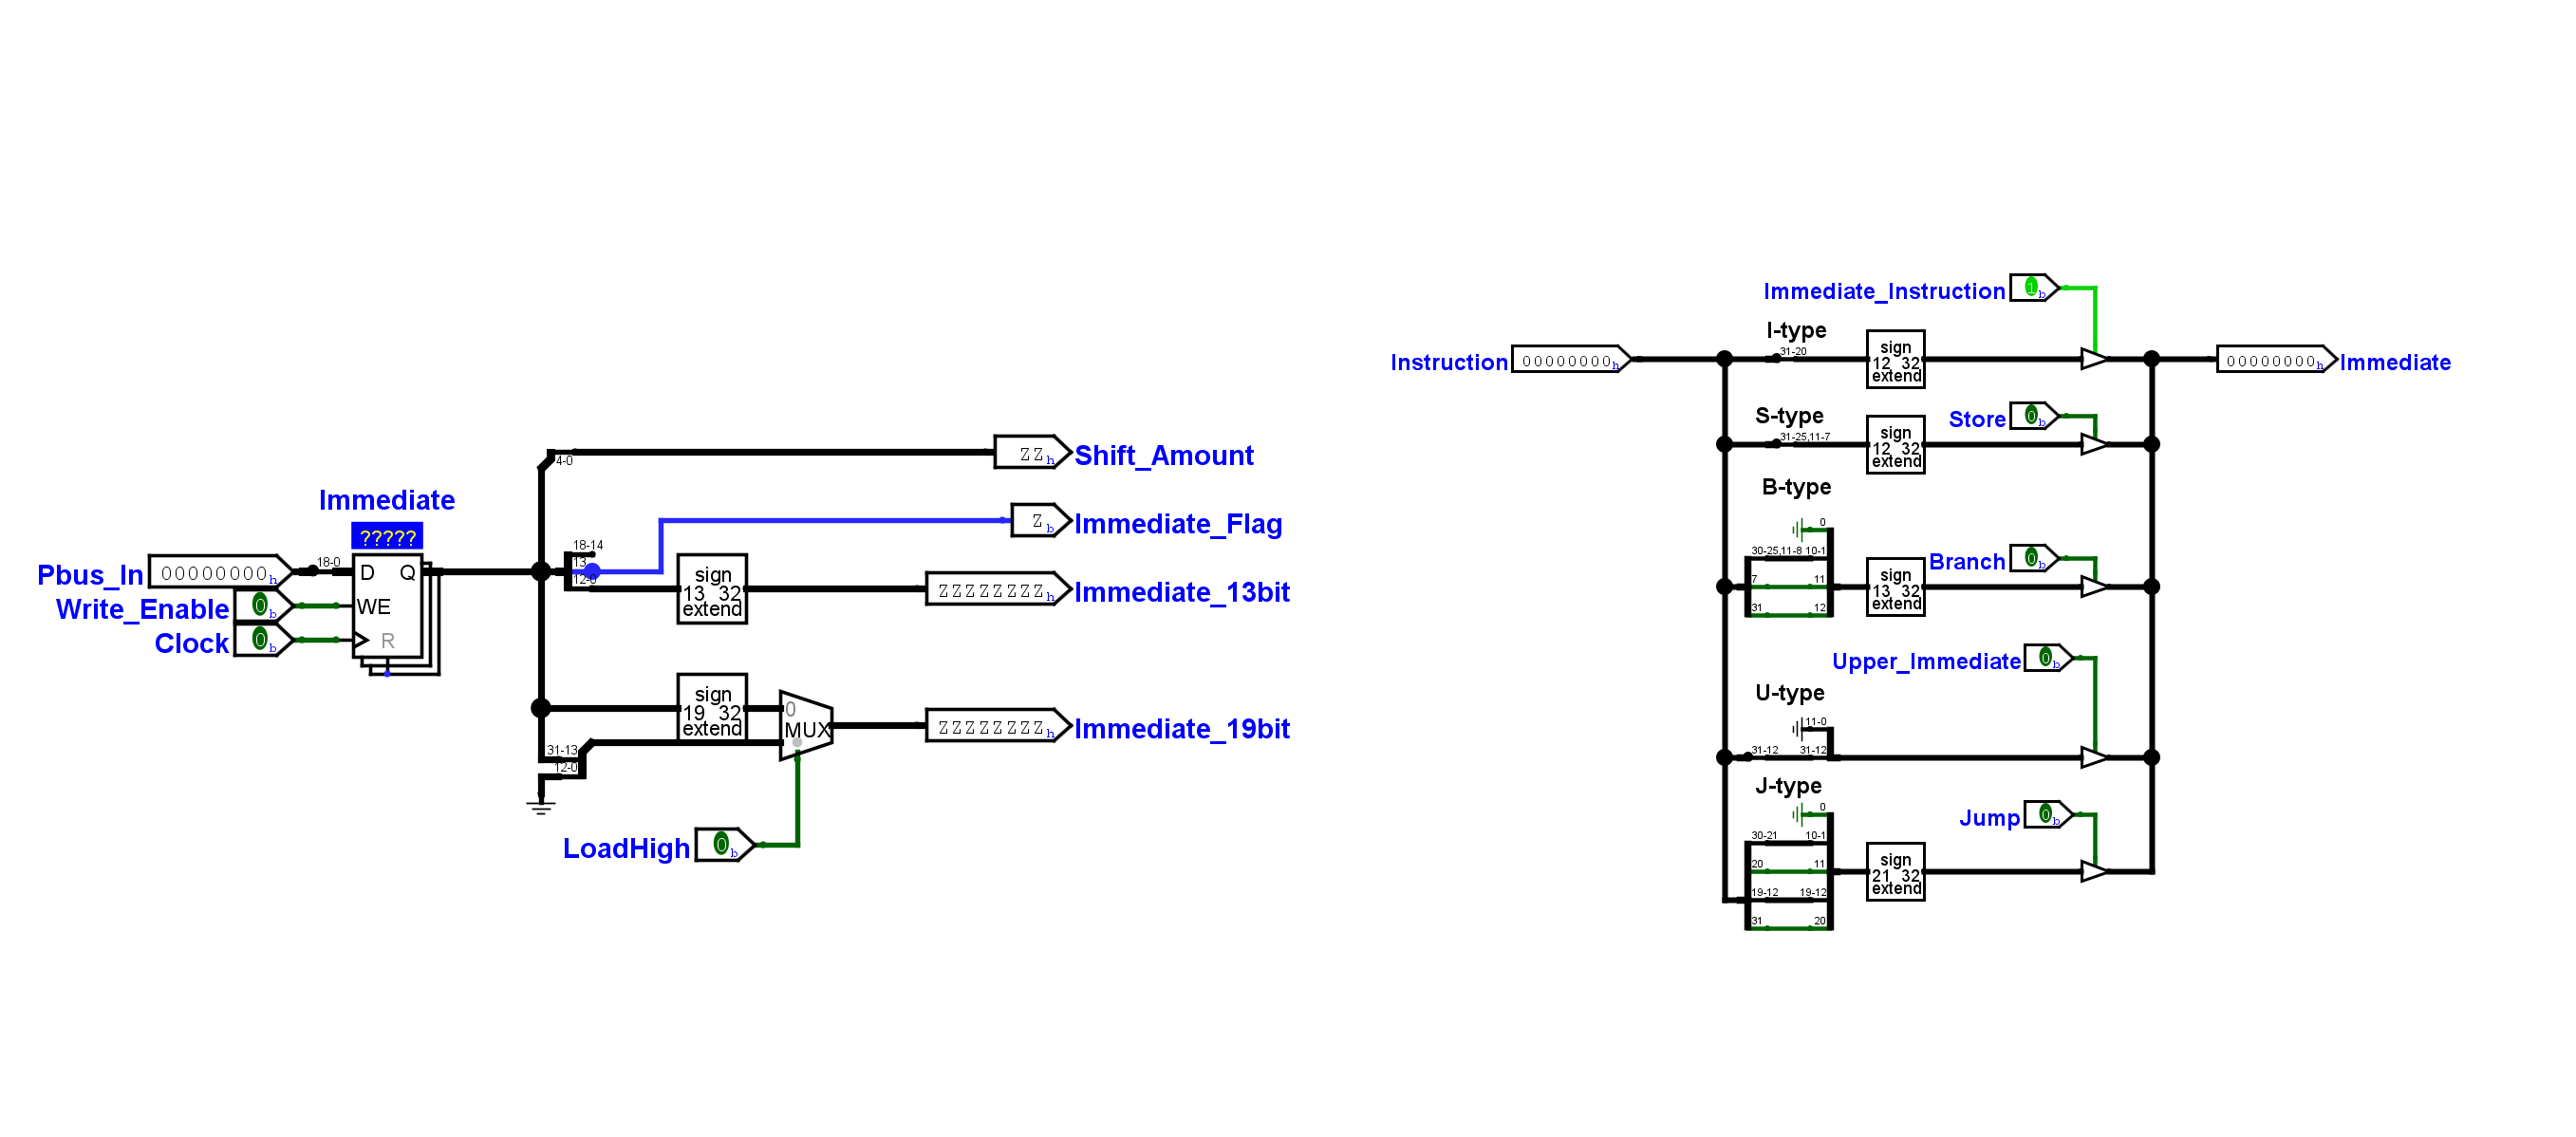
\includegraphics[width=1\linewidth]{ProcessoDesenvolvimento/Arquitetura/Immediates1.png}
    \caption{Decodificador de imediato do RISC~I(esquerda) em comparação com o novo decodificador(direita)}
    \label{fig:immediates1}
\end{figure}

O recurso de pulos condicionais(\ref{recursos_branch}) também foi adicionado durante esta fase. O RISC~I possuía pulos condicionais que dependiam de duas instruções, uma para o cálculo do código CNZV(geralmente subtração), e outra para decodificar este código e realizar o pulo caso resulte em um valor verdadeiro(instrução JUMP). 
O RISC-V, por outro lado, utiliza uma forma mais direta de pulo condicional utilizando a instrução BRANCH. Nessa instrução tanto a subtração quanto o teste de condição e execução do pulo ocorrem no mesmo ciclo. Para que isso fosse possível, uma segunda ULA com apenas adição conectada ao Contador de Programa foi criada e nomeada da ULA de Endereços(\textit{Address ALU}). Além disso o código CNZV é passado da ULA diretamente para o Controlador, onde um novo decodificador de condição é utilizado.

O novo Decodificador de Condição possui menos condições que o do RISC~I, pois diversas das condições podem ser sintetizadas alterando a ordem dos operadores. Essa diferença reduz o circuito necessário para decodificação e controle, o que pode ser observado nas Figuras \ref{fig:Controlador_1_2} e \ref{fig:condition_decoder};

\begin{figure}[h]
    \centering
    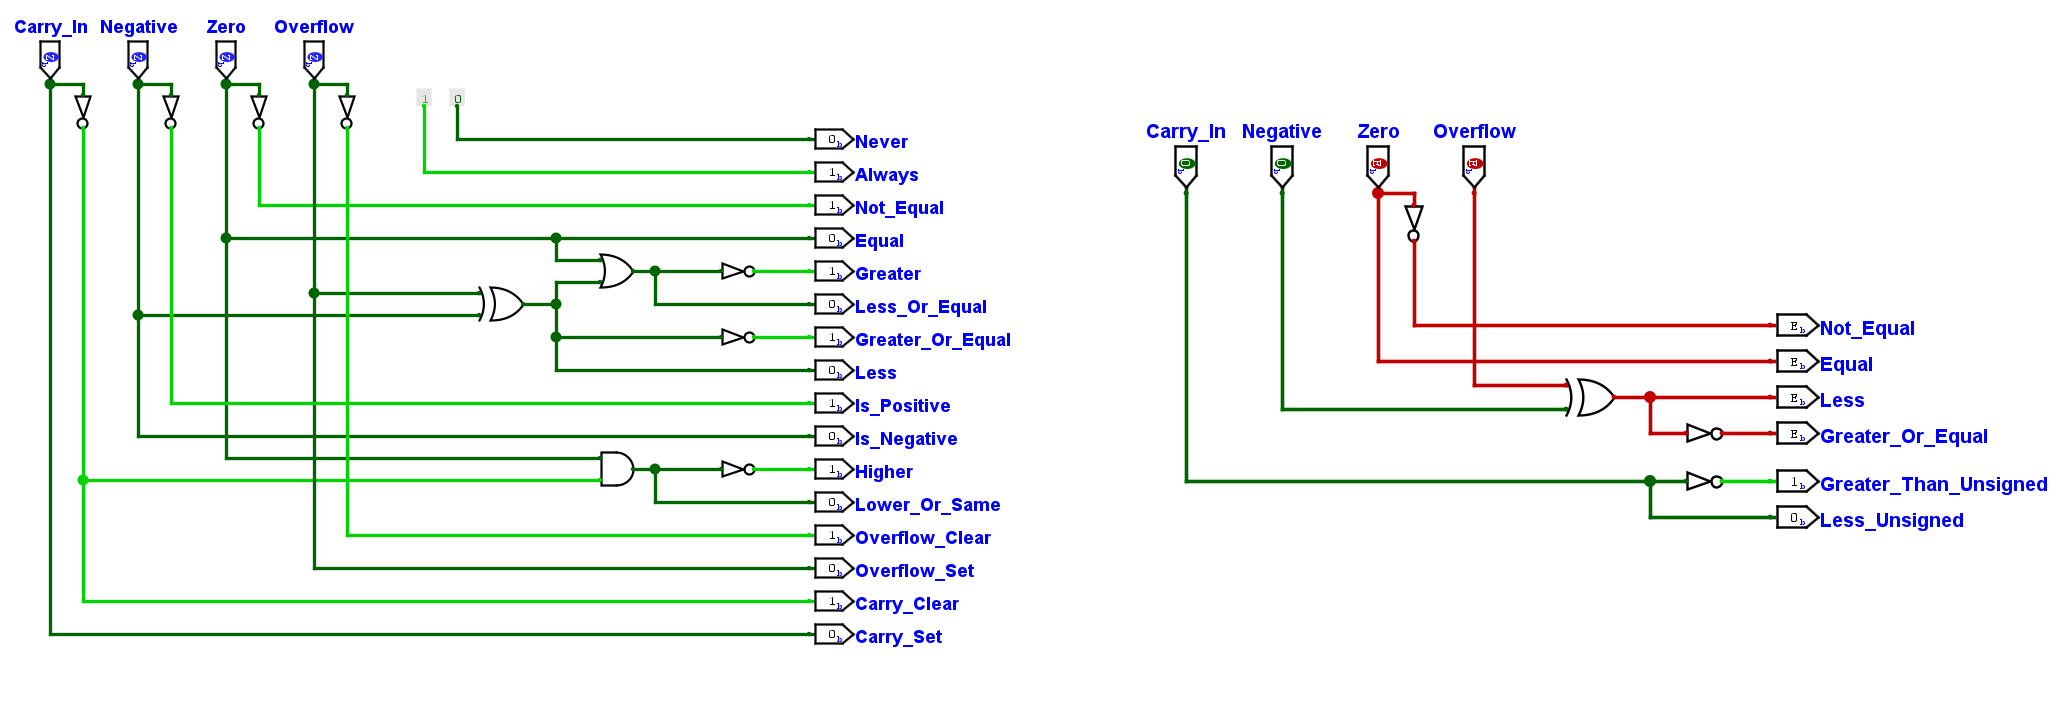
\includegraphics[width=1\linewidth]{ProcessoDesenvolvimento/Arquitetura/condition_decoder.png}
    \caption{Decodificador de condição antigo(esquerda) e novo(direita)}
    \label{fig:condition_decoder}
\end{figure}

Outras modificações foram executadas durante essa fase para adaptar o circuito ao novo controle. A ULA, não precisa mais da entrada \textit{carry in} e os valores imediatos agora são passados por apenas uma entrada, operações de Multiplicação e Divisão(\ref{recursos_muldiv}) foram adicionadas, apesar de que, nos passos seguintes a divisão foi removida, e finalmente o seu controle foi atualizado.

O Deslocador sofreu uma pequena alteração na entrada de operação(que também foi alterada na ULA), e teve a sua saída para o barramento L movida para fora do componente, o que será pertinente para alterações em passos seguintes.

Por fim foi removido o controle da entrada de endereço do Contador de Programa, que no momento, recebia o valor a ULA de Endereços. Todas as alterações dessa fase podem ser vistas na Figura~\ref{fig:desenvolvimento_arquitetura1}, com o resultado final mostrado na Figura~\ref{fig:desenvolvimento_arquitetura2}. Vale notar que nesse momento a implementação do conjunto de instruções não estava completa, pois ainda não possuía instruções de sistema(\textit{SYSTEM}), além de diversos recursos privilegiados da especificação.

\begin{figure}[H]
    \centering
    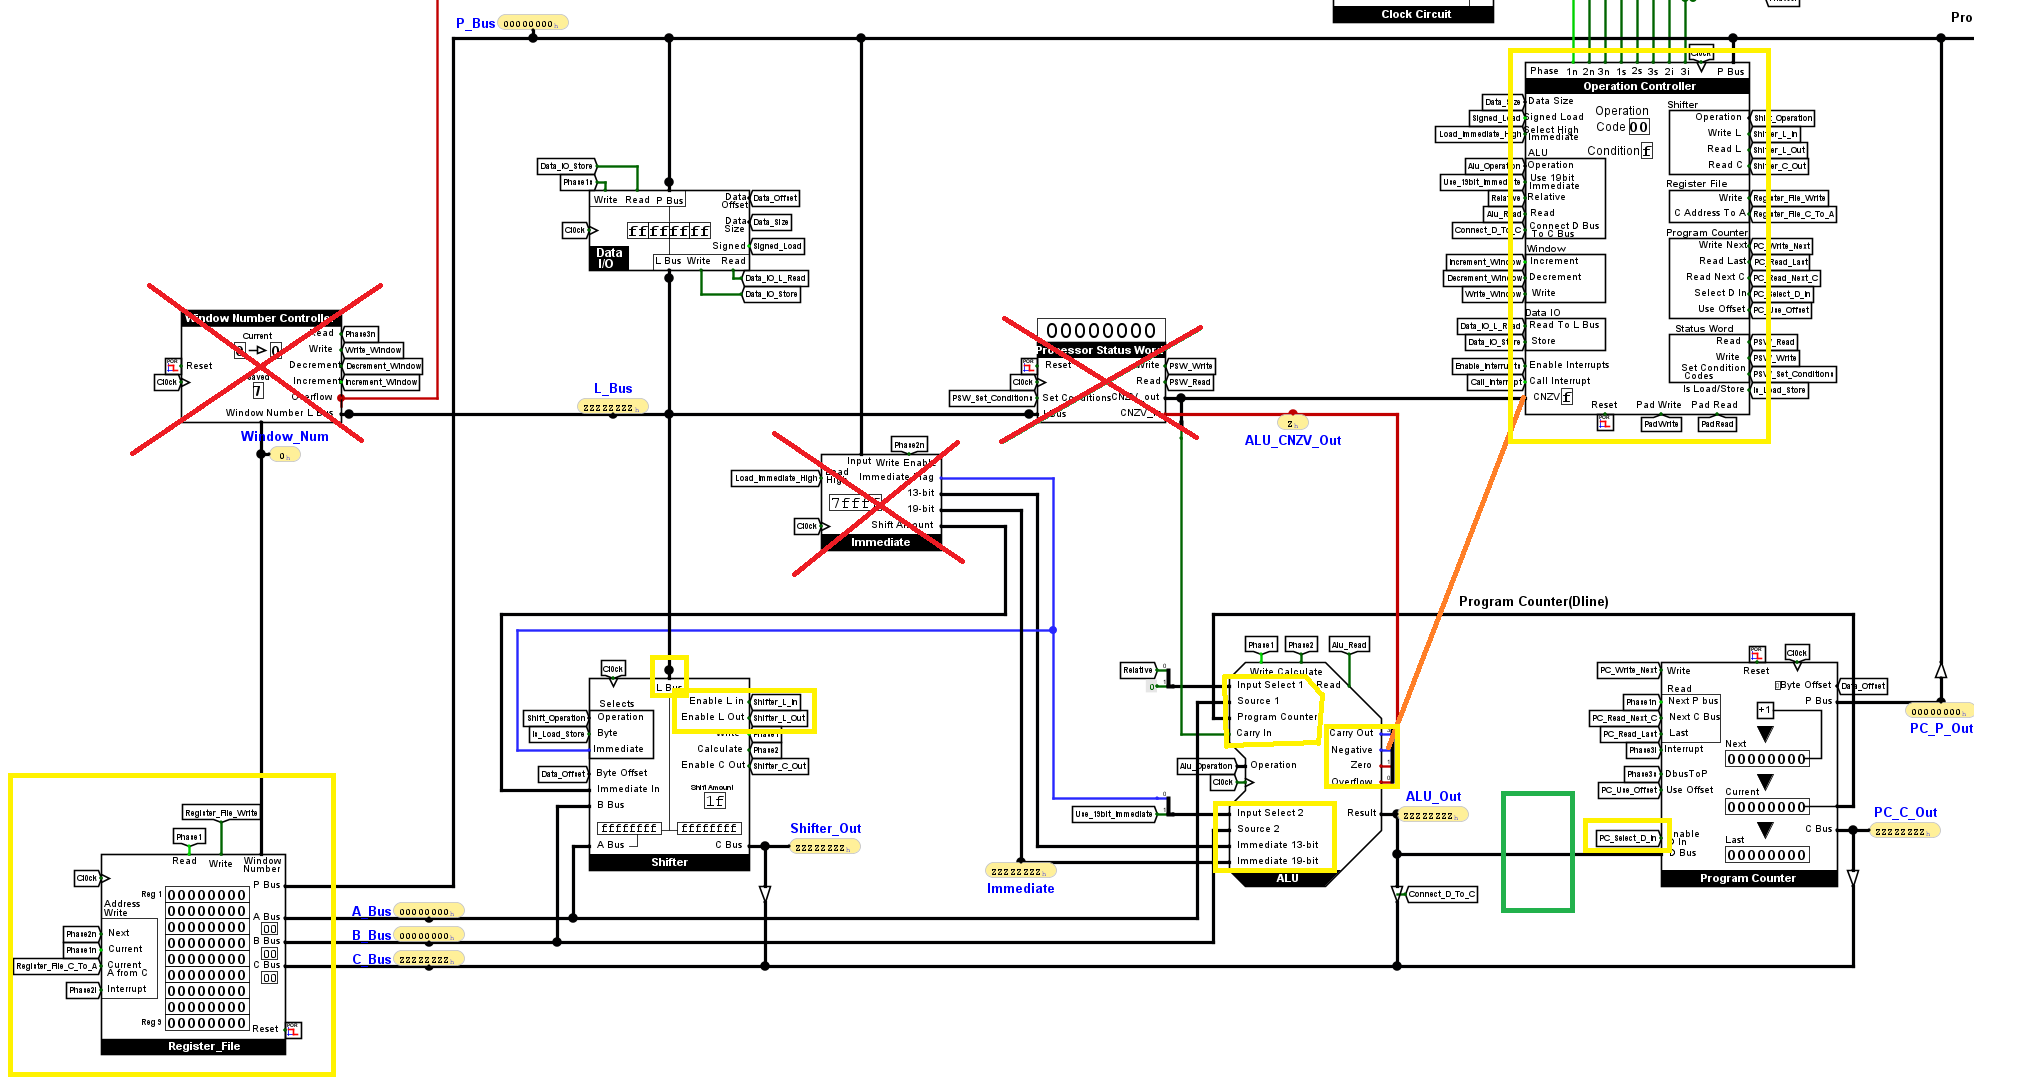
\includegraphics[width=0.9\linewidth]{ProcessoDesenvolvimento/Arquitetura/arquitetura1.png}
    \caption{Modelo original com modificações que foram executadas destacadas em amarelo, componentes que foram removidos cortados em vermelho e posições de novos componentes destacados em verde}
    \label{fig:desenvolvimento_arquitetura1}
\end{figure}
\begin{figure}[H]
    \centering
    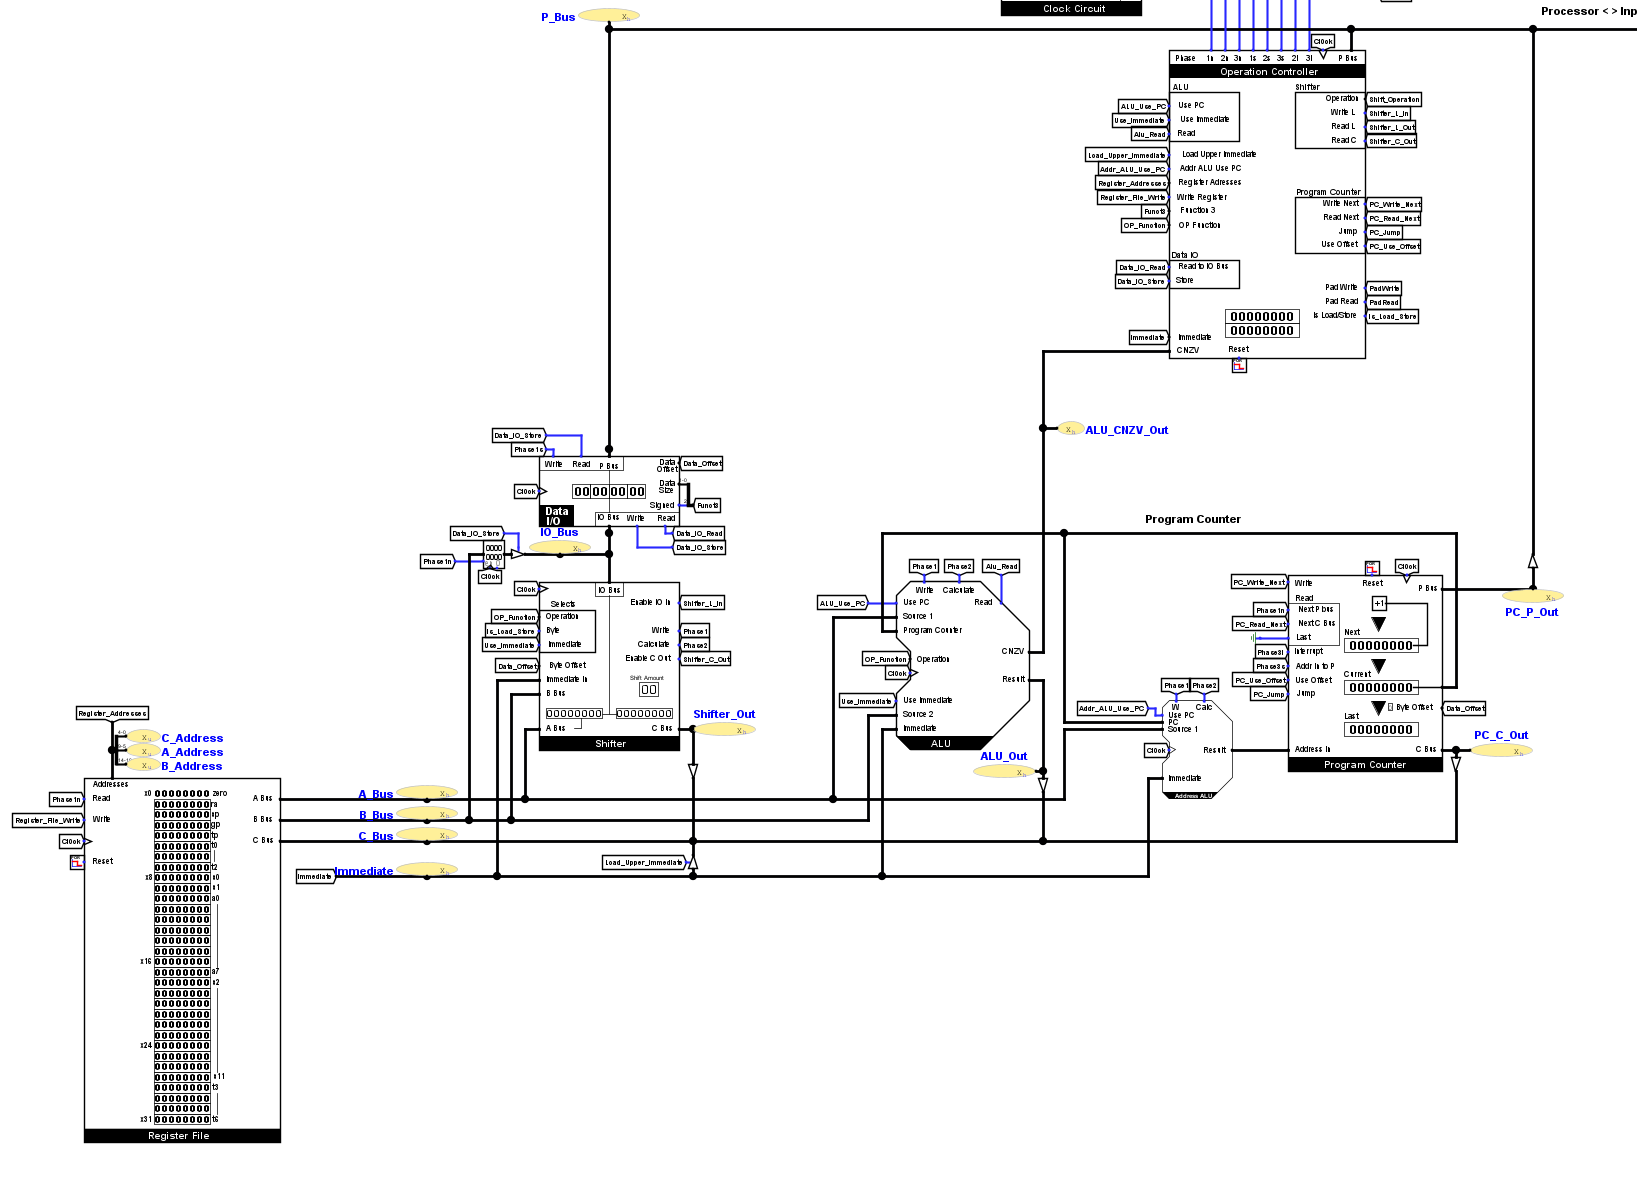
\includegraphics[width=0.9\linewidth]{ProcessoDesenvolvimento/Arquitetura/Arquitetura2.png}
    \caption{Resultado da primeira fase de modificações da arquitetura}
    \label{fig:desenvolvimento_arquitetura2}
\end{figure}


\subsubsection{Segunda Fase: \textit{Pipeline} e Usabilidade}

Após as primeiras modificações para adaptar a arquitetura ao conjunto de instruções RISC-V, a \textit{Pipeline} da arquitetura foi analisada para melhorias. No RISC~I \cite{peek_vlsi_1983}, a \textit{Pipeline} funciona em uma divisão de dois estágios que ocorrem durante três ciclos de \textit{clock}, chamados de fases.

No primeiro estágio (I), ocorre a coleta da próxima instrução (\textit{Instruction Fetch} ou IF) durante a fase 2n e a decodificação da instrução coletada anteriormente (\textit{Instruction Decode} ou ID) durante a fase 1n. Após este estágio (E), uma sequência de operações ocorre, começando pela passagem de operandos, que saem do Arquivo de Registradores para os outros componentes através dos barramentos A e B, que então podem ser usados em operações matemáticas durante a fase 2n (\textit{Execution} ou EX).

Para qualquer instrução que não acesse a memória, o segundo estágio termina na fase 3n, onde os resultados de quaisquer operações são escritos no Arquivo de Registradores através do barramento C (\textit{Write Back} ou WB). Porém, caso a instrução acesse a memória, o segundo estágio é estendido. Essa extensão (D) envia o endereço que deve ser acessado na memória e então carrega ou envia os dados que precisam ser trocados (\textit{Memory} ou MEM).

\begin{figure}[h]
    \centering
    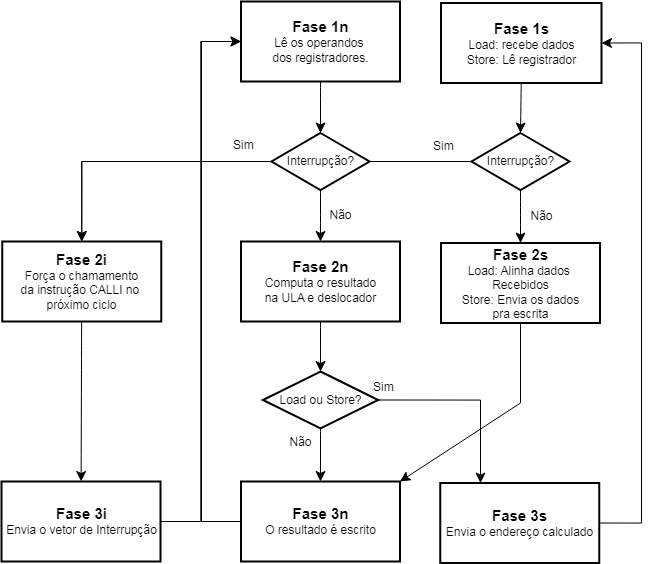
\includegraphics[width=0.5\linewidth]{ProcessoDesenvolvimento/Arquitetura/temporizacao_RISC-I.png}
    \caption{Temporização do RISC~I (adaptado de \citeonline{peek_vlsi_1983})}
    \label{fig:temporizationDiagram}
\end{figure}

Tudo isso ocorre durante as fases que possuem o sufixo S, que podem ser vistas no fluxograma na Figura~\ref{fig:temporizationDiagram}, mostrando todas as possíveis fases que ocorrem durante o segundo estágio. As fases adicionais, com sufixo I, referem-se ao tratamento de interrupções; porém, como estas foram removidas durante a fase de desenvolvimento anterior, elas podem ser ignoradas.

A Figura~\ref{fig:pipelineRISCI} mostra como as instruções são divididas e executadas utilizando a \textit{Pipeline} do RISC~I. Dentro das divisões mostradas, o I corresponde ao primeiro estágio (IF + ID), o E corresponde ao segundo estágio (EX + WB) enquanto o estágio D corresponde à extensão que ocorre durante as instruções de carregamento e armazenamento (MEM).

\begin{figure}[h]
    \centering
    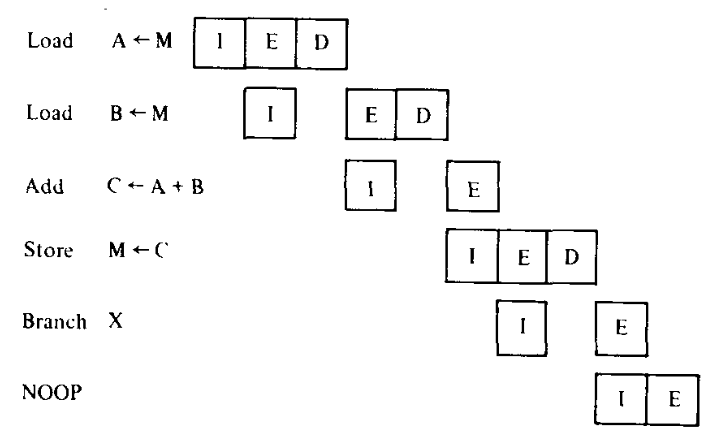
\includegraphics[width=0.5\linewidth]{ProcessoDesenvolvimento/Arquitetura/pipelineRISCI.png}
    \caption{Demonstração da \textit{pipeline} do RISC~I.\cite{stallings_reduced_1988}}
    \label{fig:pipelineRISCI}
\end{figure}

É visível que, em instruções que acessam a memória, a extensão de carregamento atrasa a coleta, decodificação e execução em um estágio da pipeline, tornando acessos à memória ineficientes na execução de programas. Durante o desenvolvimento do RISC~II, isso foi corrigido, o que fez a extensão de acesso à memória ser executada em paralelo com os outros estágios da pipeline, conforme mostrado na Figura~\ref{fig:pipelineRISCII}.

\begin{figure}[h]
    \centering
    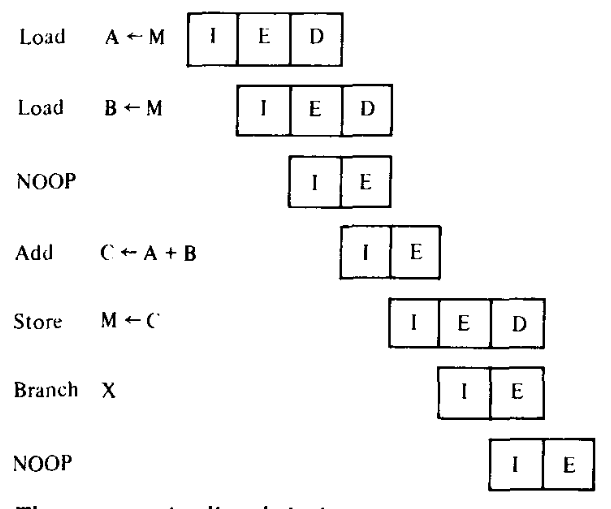
\includegraphics[width=0.5\linewidth]{ProcessoDesenvolvimento/Arquitetura/PipelineRISCII.png}
    \caption{Demonstração da \textit{pipeline} do RISC~II.\cite{stallings_reduced_1988}}
    \label{fig:pipelineRISCII}
\end{figure}

Neste momento, essa modificação pareceu simples o suficiente para ser implementada na arquitetura, o que levou à sua execução (\ref{recursos_pipe3}). A \textit{Pipeline} poderia ser revisitada no futuro, dividindo os passos de IF e ID, e os passos de EX e WB, tornando-a uma \textit{Pipeline} de cinco estágios.

O primeiro passo dessa modificação foi remover completamente o componente de Controle de \textit{Clock}. Este componente já não possuía mais função na arquitetura, pois, com o sistema de interrupções removido e a eliminação da extensão nas instruções \texttt{load} e \texttt{store}, as únicas fases utilizadas seriam as fases 1n, 2n e 3n, que podem ser alimentadas diretamente por um gerador de fase externo (neste momento, três componentes de \textit{Clock} com tempo e fase diferentes).

O controlador recebeu um novo registrador, que armazena a instrução executada anteriormente. Essa instrução é então decodificada entre \texttt{load} e \texttt{store}, gerando dois novos sinais de controle. Esses sinais substituem as ativações que ocorriam durante as fases S, além de gerarem uma substituição temporária do código \textit{funct3}, que define o tamanho da informação a ser carregada pelo \texttt{load}, e do endereço dos registradores, que é modificado para conter o endereço que receberá a informação de \texttt{load}.

\begin{figure}[h]
    \centering
    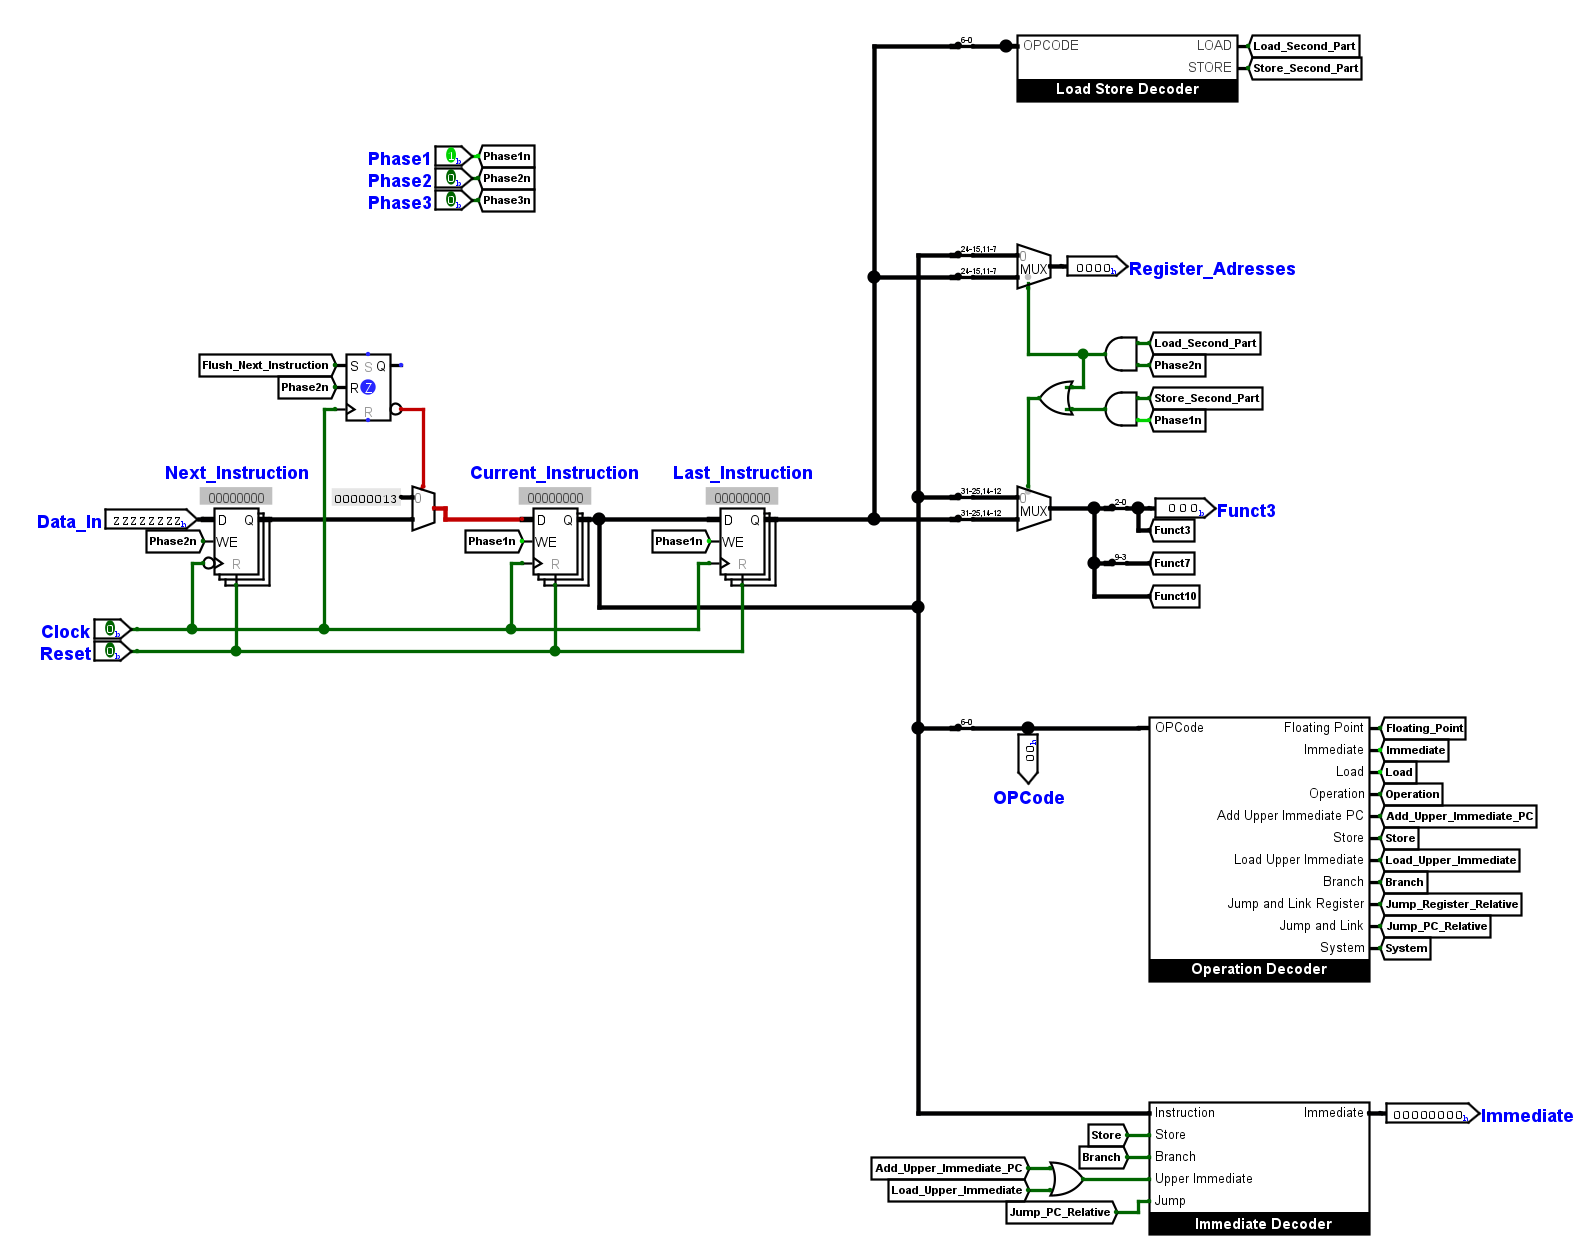
\includegraphics[width=0.5\linewidth]{ProcessoDesenvolvimento/Arquitetura/controlador_2_1.png}
    \caption{Primeira fase de decodificação durante a segunda fase de desenvolvimento}
    \label{fig:controlador_2_1}
\end{figure}

A Figura~\ref{fig:controlador_2_1} mostra o resultado das modificações realizadas na primeira fase de decodificação do Controlador. A organização dos componentes foi alterada para melhor separação e visualização. Além disso, vestígios do controle relacionado a interrupções foram removidos, e os Decodificadores de Operação e Imediato foram levemente modificados.

O Decodificador de Operação teve apenas seu encapsulamento alterado, com as saídas completamente visíveis. O Controlador de Imediato sofreu alterações mais significativas, com a substituição dos \textit{buffers tri-state} por multiplexadores para a seleção do valor de saída. Esta mudança foi feita porque FPGAs geralmente não suportam \textit{buffers tri-state} internamente. Além disso, permite que um valor padrão esteja sempre disponível; no caso, o imediato de 12 bits das instruções OP-IMM. A Figura~\ref{fig:Immediates2} mostra o resultado dessas mudanças.

\begin{figure}
    \centering
    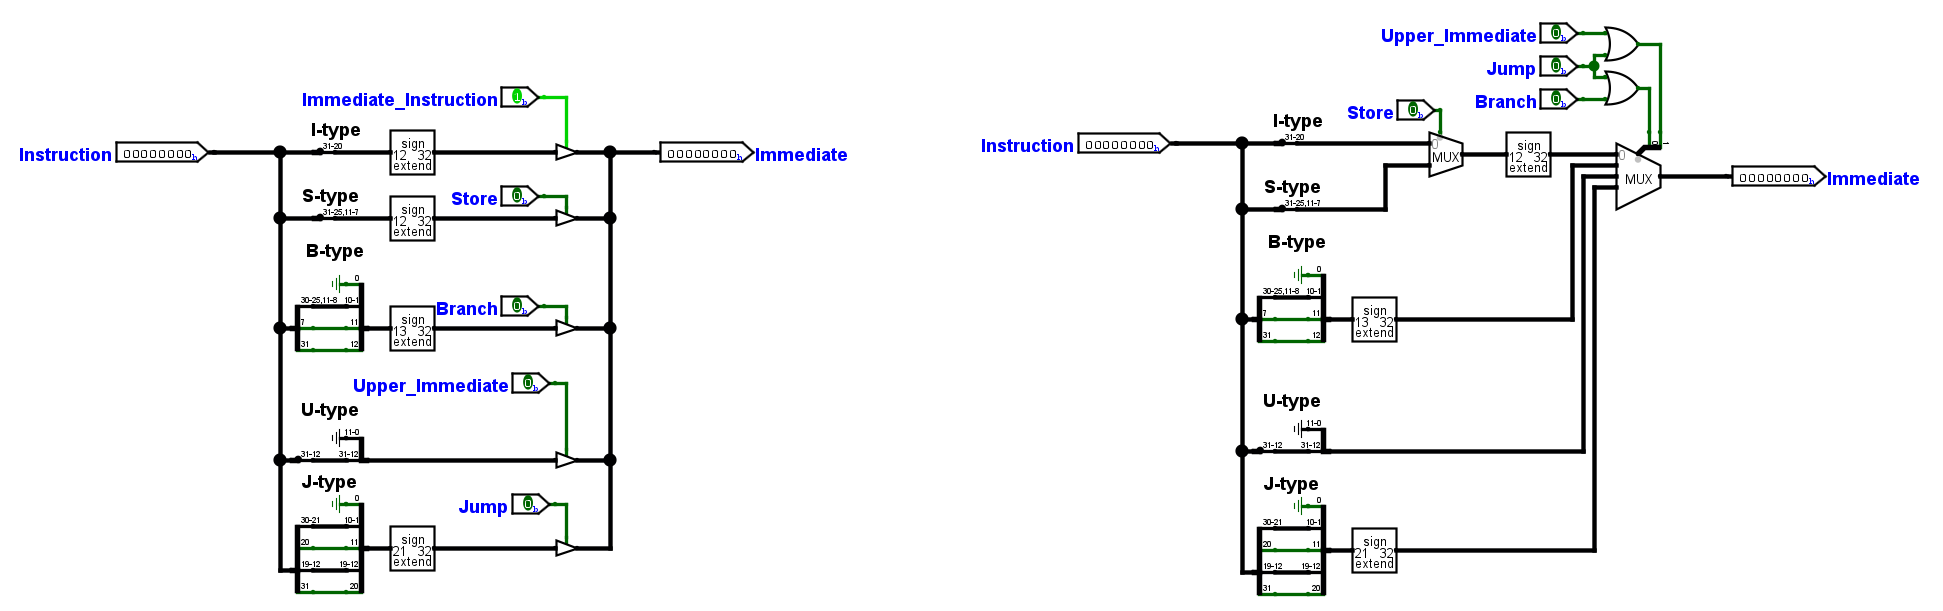
\includegraphics[width=1\linewidth]{ProcessoDesenvolvimento/Arquitetura/Immediates2.png}
    \caption{Comparação entre o Decodificador de Imediato com \textit{buffers tri-state} (esquerda) e multiplexadores (direita)}
    \label{fig:Immediates2}
\end{figure}

A Figura~\ref{fig:Controlador_2_2} mostra as alterações na segunda etapa de decodificação. Modificações adicionais relacionadas à \textit{Pipeline} incluíram o descapsulamento do decodificador de condição e alterações no controle do Deslocador e Data IO, que foram separados durante essa fase.

\begin{figure}[h]
    \centering
    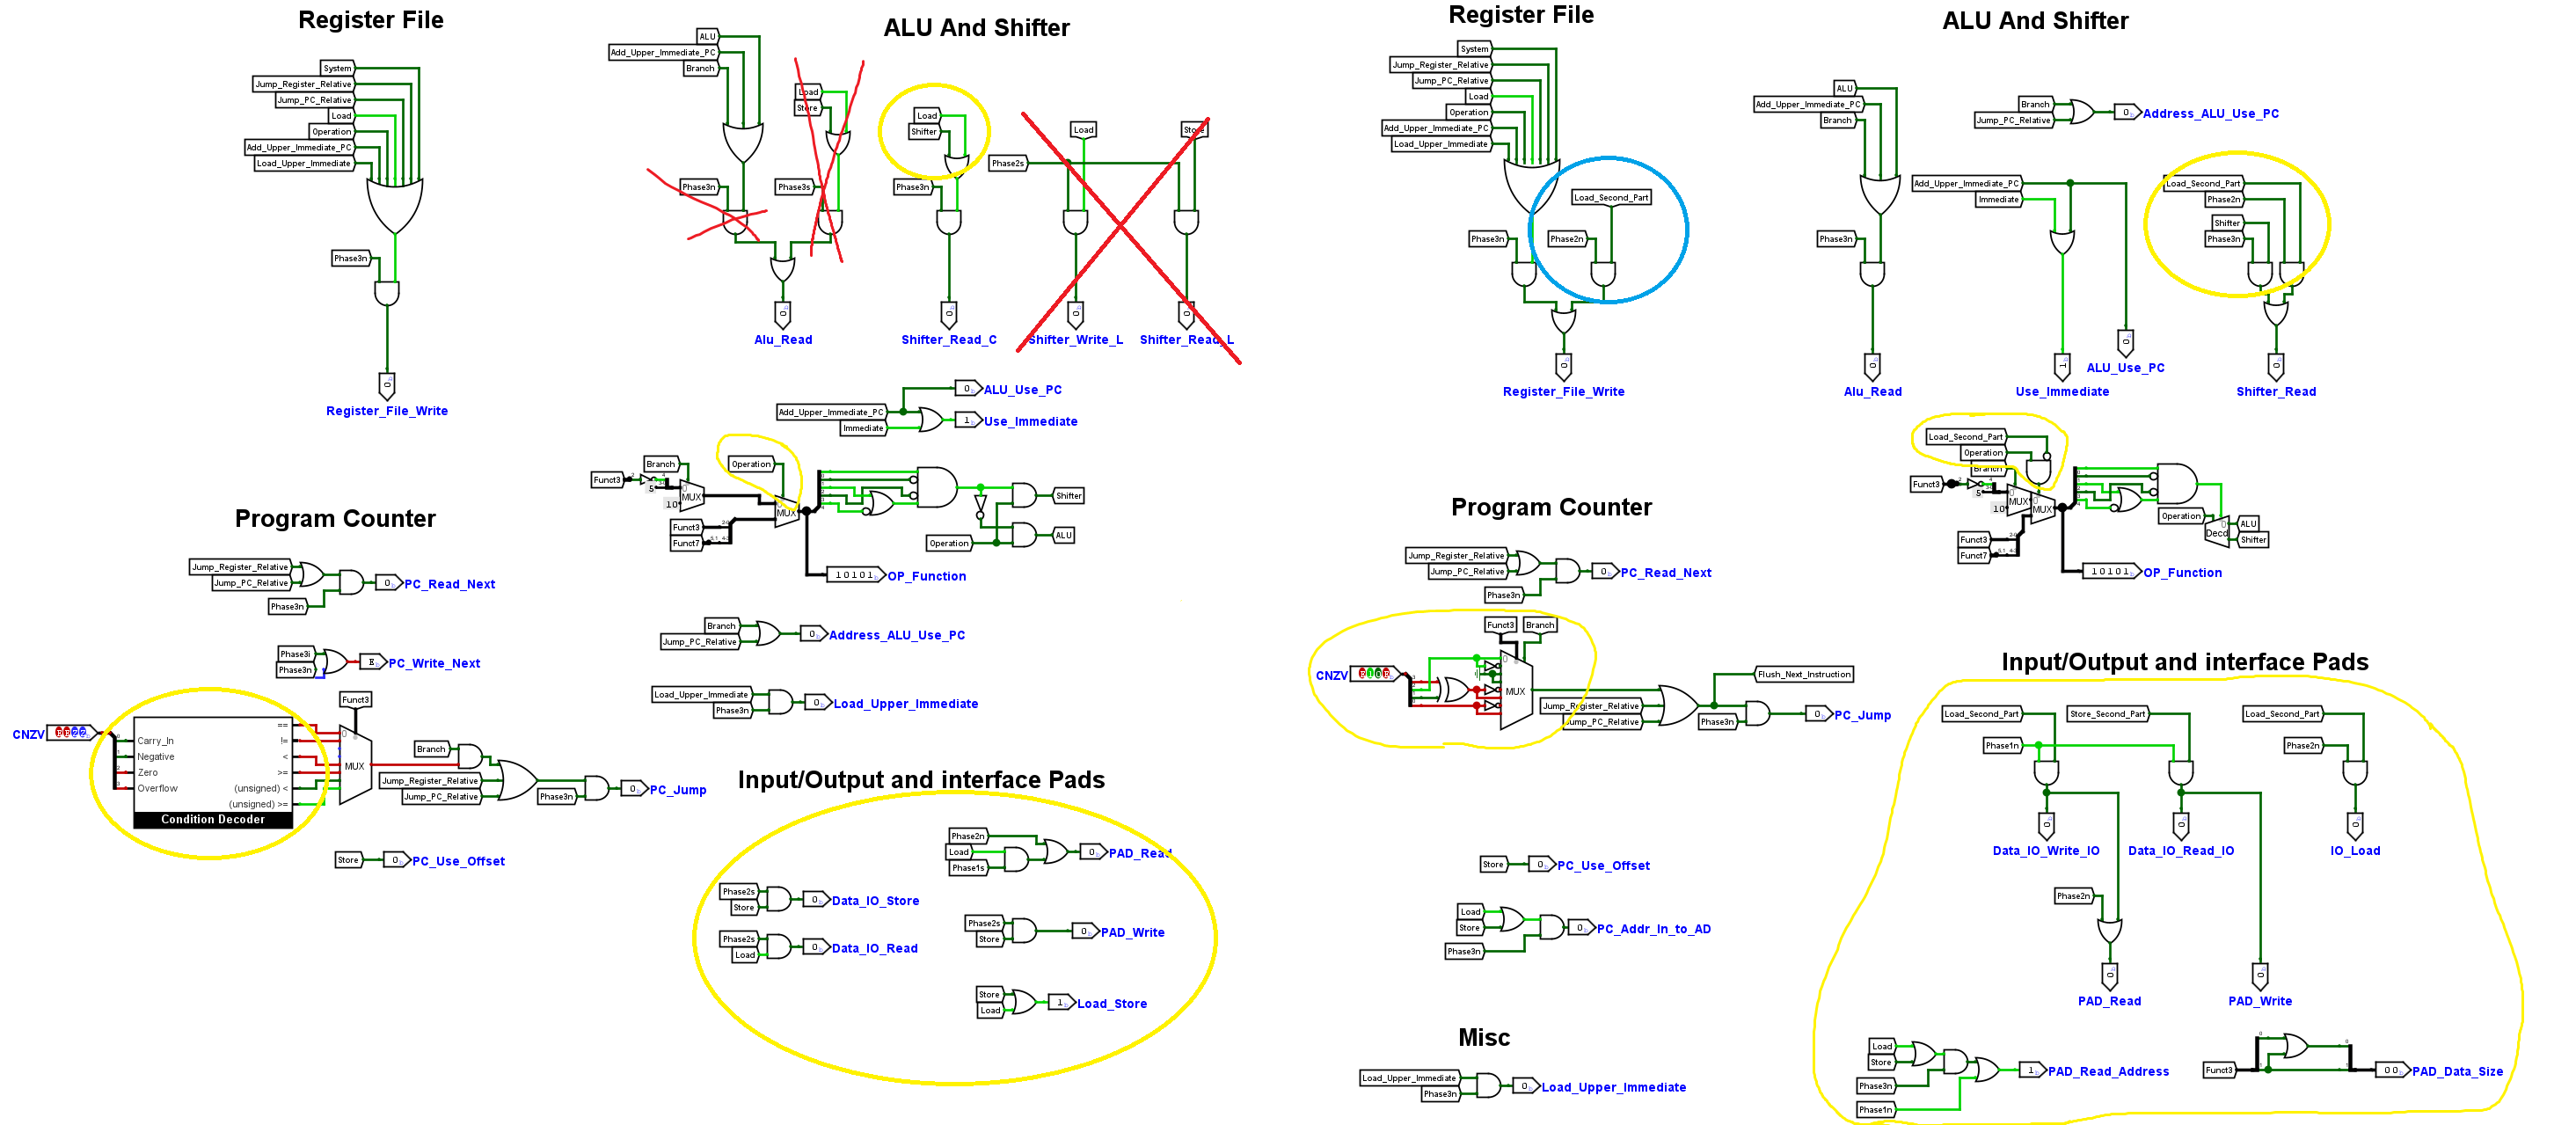
\includegraphics[width=1\linewidth]{ProcessoDesenvolvimento/Arquitetura/Controlador_2_2.png}
    \caption{Segunda fase de decodificação de instruções. Antes (esquerda) Depois (direita)}
    \label{fig:Controlador_2_2}
\end{figure}

Neste estágio do desenvolvimento, mesmo após testes, um erro na decodificação do \textit{OP\_Function} passou despercebido. O sinal da segunda fase do carregamento afetava a \textit{Pipeline} durante toda a fase, quando deveria afetar apenas o segundo ciclo de \textit{clock}. Esse erro foi corrigido em etapas posteriores.

O recurso de \textit{Pipeline Flush} (\ref{recursos_pipe_flush}) foi adicionado para eliminar os \textit{hazards} relacionados à execução de saltos como pode ser visto nas Figuras \ref{fig:controlador_2_1} e \ref{fig:Controlador_2_2}(Acima da saída \textit{PC\_Jump}). No entanto, considerou-se que esse recurso poderia ser removido em favor de soluções mais eficientes, como predição de salto.

Para tornar a visualização da arquitetura mais amigável, foi realizada uma melhoria visual dos componentes, destacando e separando melhor as entradas e exibindo registradores que antes só poderiam ser vistos inspecionando os componentes. Todas as alterações podem ser vistas na Figura~\ref{fig:AtualizacaoVisual}.

\begin{figure}[ht]
    \centering
    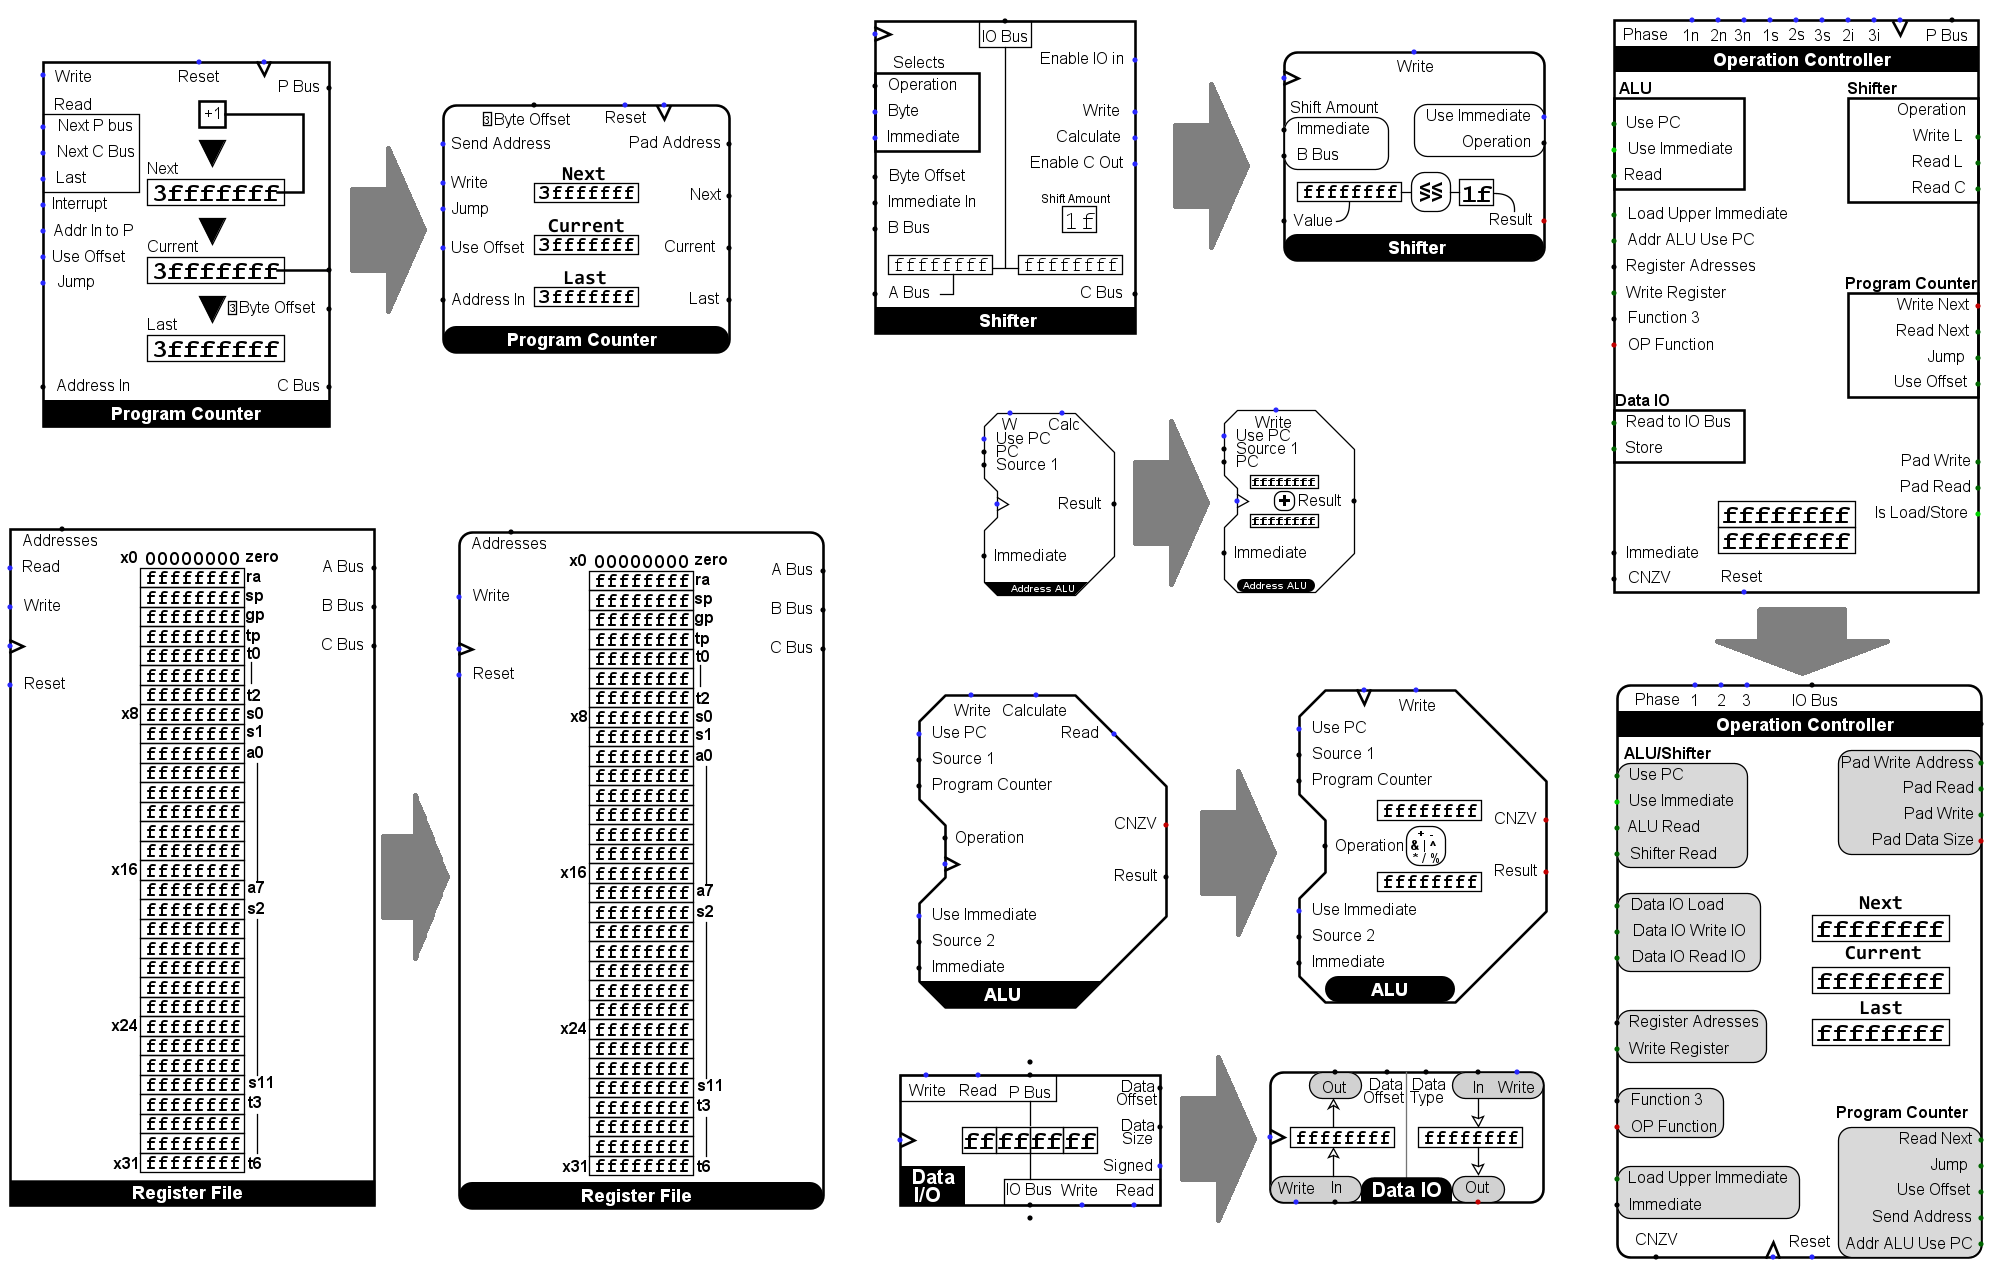
\includegraphics[width=1\linewidth]{ProcessoDesenvolvimento/Arquitetura/ComponentsVisualUpdate.png}
    \caption{Atualização no visual dos componentes}
    \label{fig:AtualizacaoVisual}
\end{figure}

A Figura~\ref{fig:AtualizacaoVisual} também mostra a remoção dos sinais de cálculo e leitura. A ULA e o Deslocador possuíam registradores que armazenavam o resultado das operações, mas essa armazenagem não era necessária, pois o valor fica disponível até que os registradores de entrada sejam atualizados, permitindo tempo suficiente para ser escrito no Arquivo de Registradores. Essa remoção simplificou tanto a estrutura interna quanto os sinais de controle necessários para a execução.

Os sinais de leitura foram movidos para fora dos componentes, controlando agora uma série de multiplexadores conectados ao barramento C. A motivação dessa alteração foi a mesma realizada no Decodificador de Imediato, tornando o sistema mais compatível com FPGAs. As modificações podem ser vistas na Figura~\ref{fig:Arquitetura3}.

\begin{figure}[ht]
    \centering
    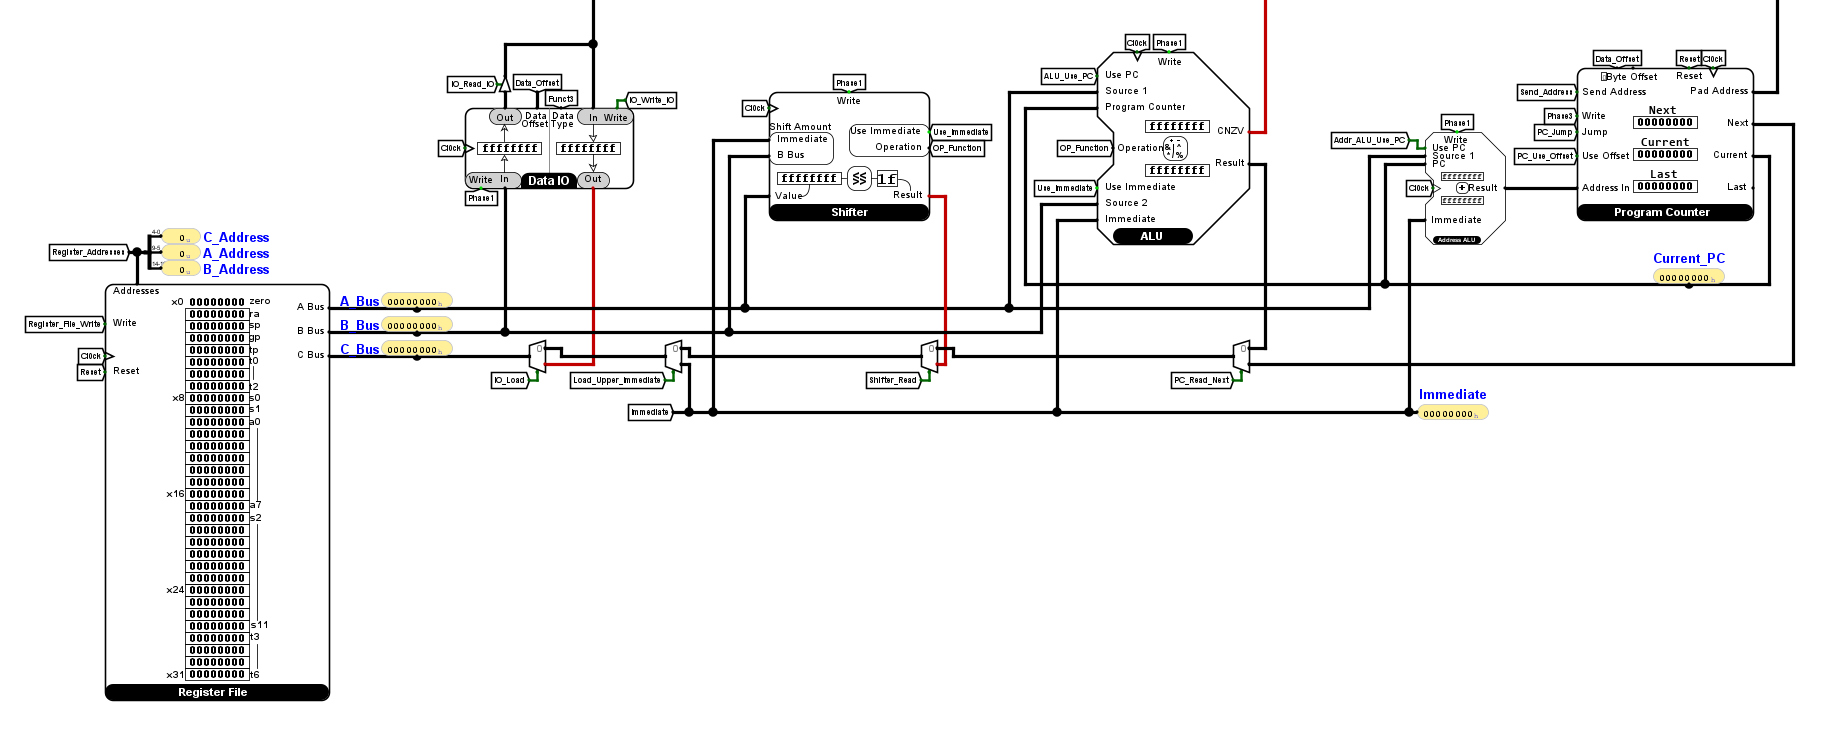
\includegraphics[width=1\linewidth]{ProcessoDesenvolvimento/Arquitetura/Arquitetura3.png}
    \caption{Visualização dos componentes e suas conexões com os barramentos}
    \label{fig:Arquitetura3}
\end{figure}

Além disso, foi realizada a separação entre o \textit{DataIO} e o Deslocador. No RISC~I, esses componentes trabalham em conjunto durante as instruções de \texttt{load} e \texttt{store}, pois a informação recebida nas instruções de carregamento às vezes precisa ser deslocada. No entanto, essa integração adiciona complexidade ao controle e pode causar problemas futuros. 

\begin{figure}[h]
    \centering
    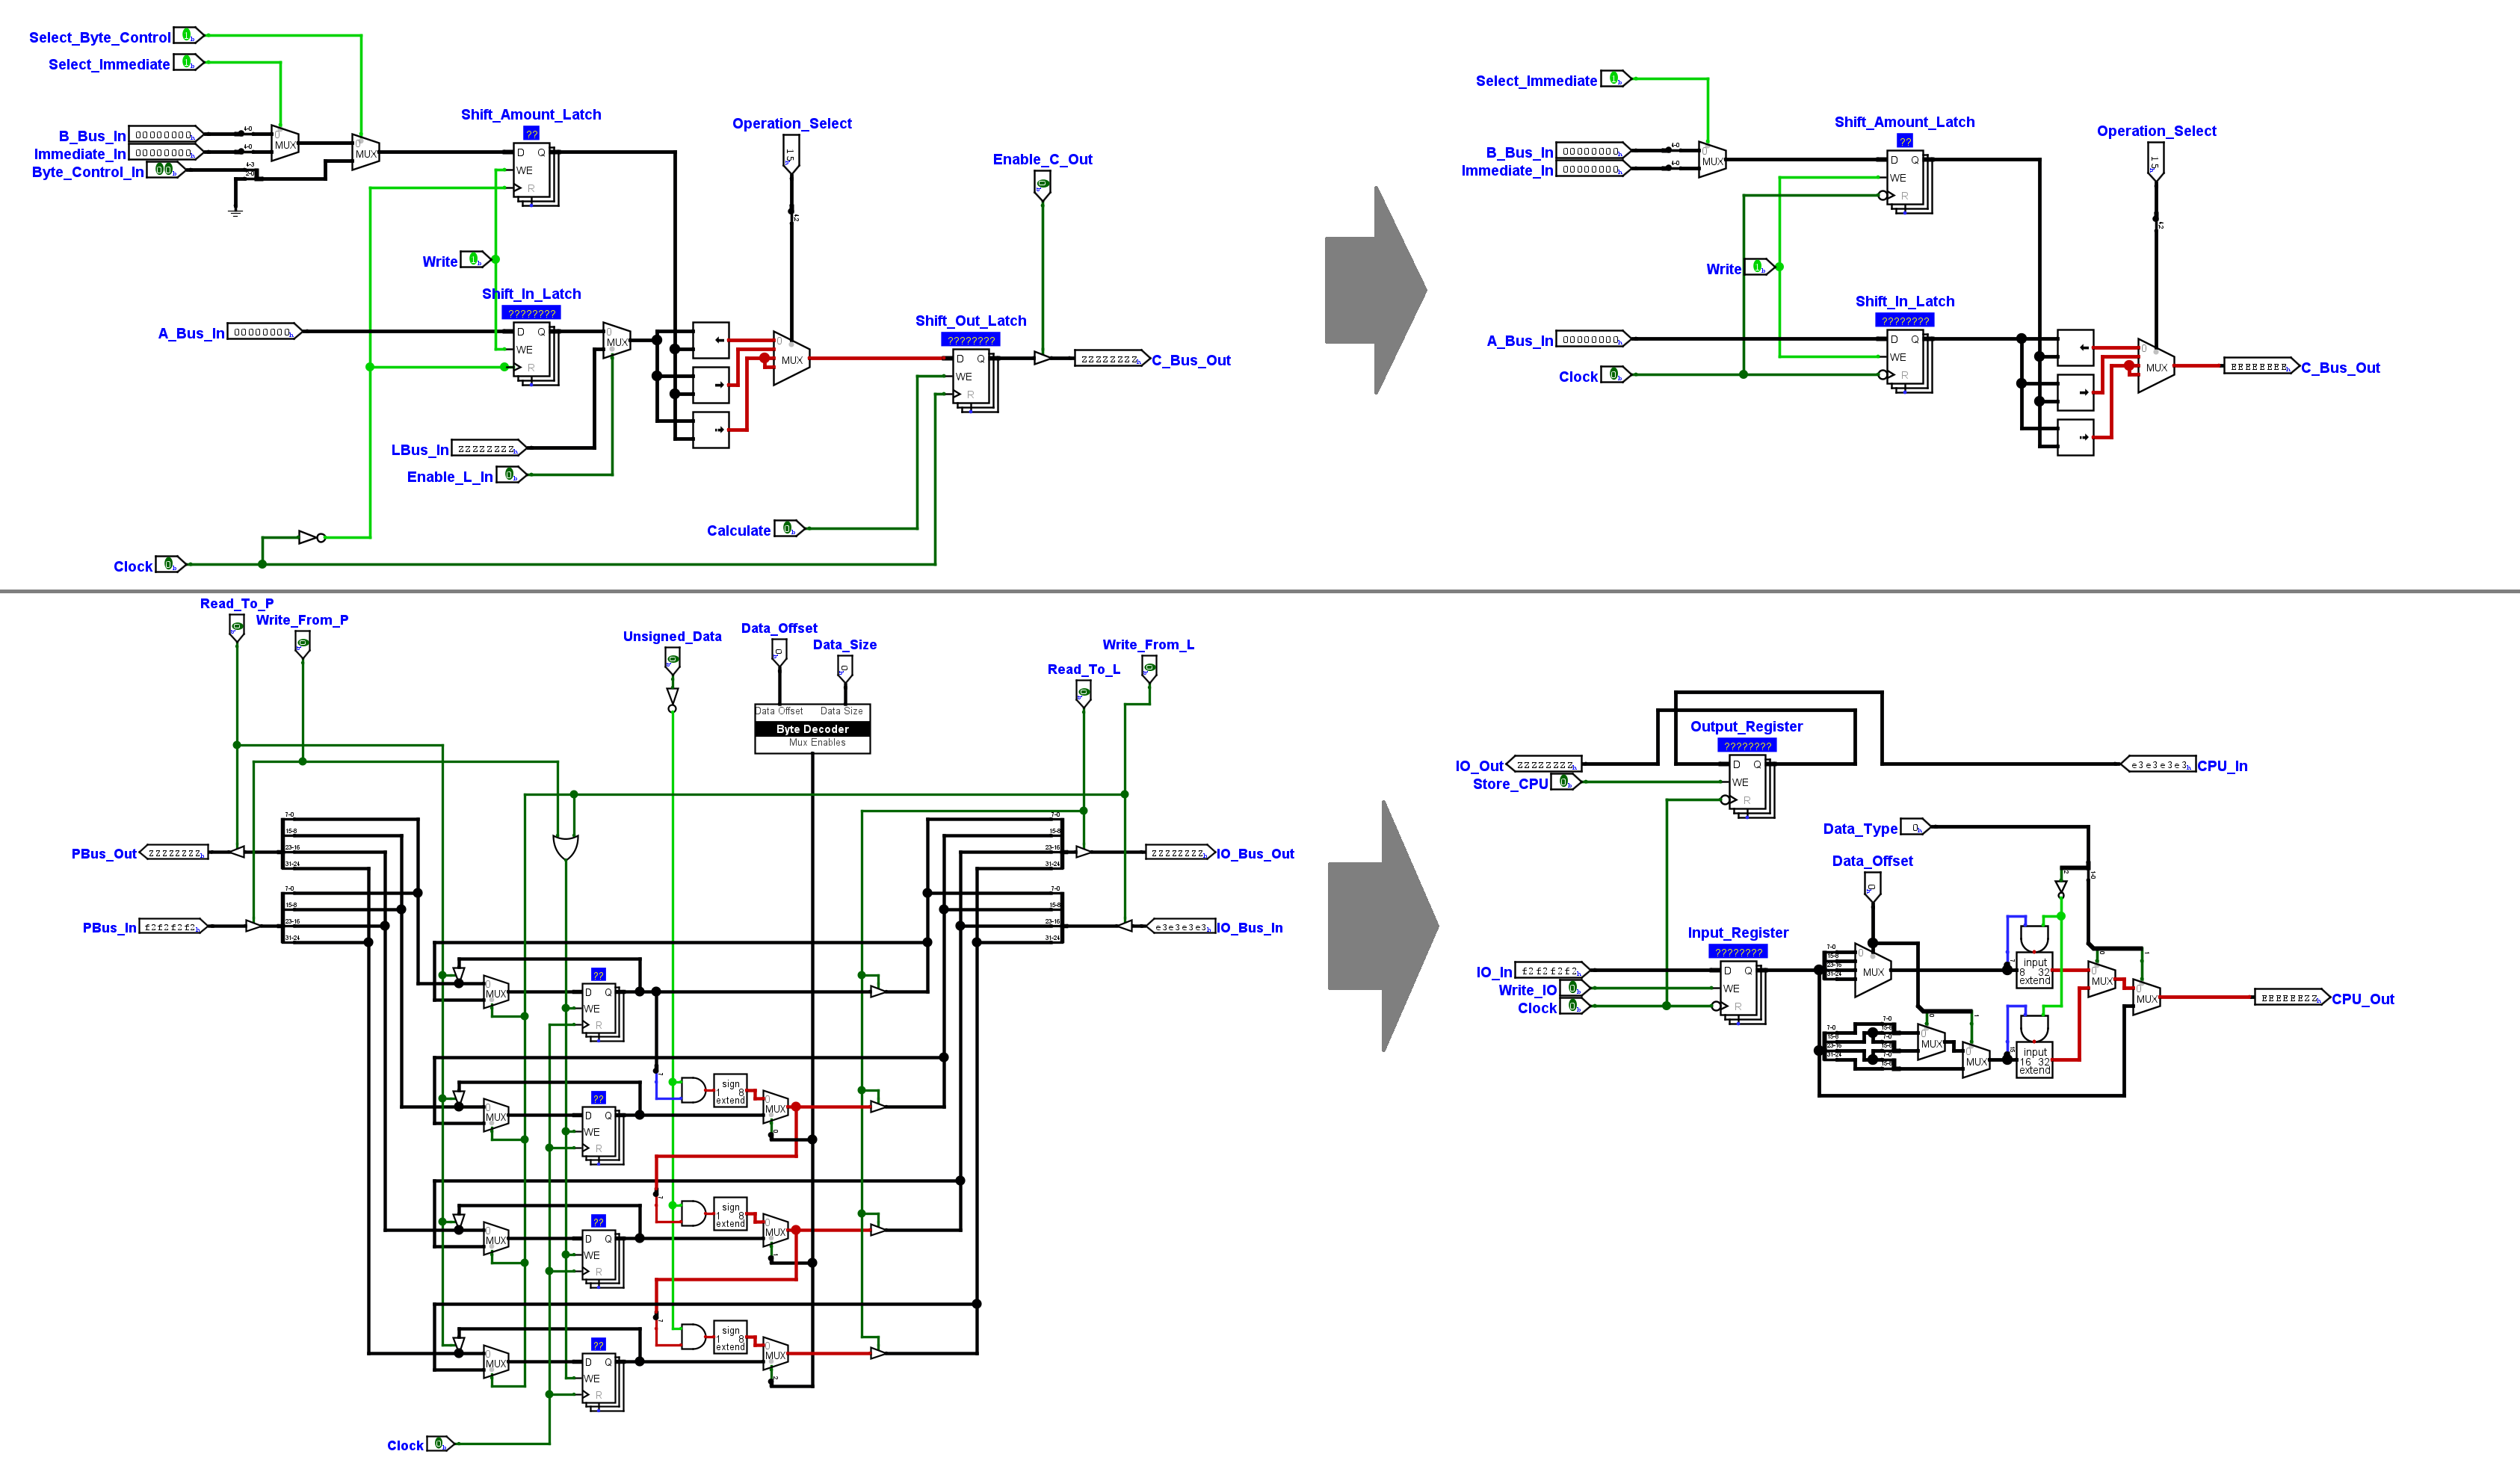
\includegraphics[width=1\linewidth]{ProcessoDesenvolvimento/Arquitetura/ShifterIOoldnew.png}
    \caption{Comparação entre o Deslocador (acima) e o DataIO (abaixo) antes e depois}
    \label{fig:ShifterIOoldnew}
\end{figure}

A Figura~\ref{fig:ShifterIOoldnew} mostra que houve uma grande redução no circuito do Deslocador, enquanto o \textit{DataIO}, apesar da redução visual, pode ter aumentado em complexidade devido à necessidade de mais multiplexadores com um maior número de entradas. Agora, o \textit{DataIO} precisa realizar o deslocamento necessário.

Além dessa separação, o \textit{DataIO} teve os registradores utilizados durante o \texttt{load} e \texttt{store} e os caminhos dos dados carregados e salvos separados. Essa alteração, embora não estritamente necessária, facilita a compreensão do fluxo de dados no circuito.

A saída dos dados para o barramento P (agora chamado barramento de IO ou barramento de dados) ainda possuía um \textit{buffer tri-state}, mas a remoção desse componente estava planejada.

No Contador de Programas, pequenas alterações foram feitas. O primeiro registrador foi alterado para um contador, o que simplifica visualmente os componentes, facilitando o entendimento do que está acontecendo. A saída para o barramento C foi trocada por uma saída para cada registrador, transferindo o controle de seleção para componentes externos. Essas alterações podem ser vistas na Figura~\ref{fig:ContadorDePrograma1}.

\begin{figure}[t]
    \centering
    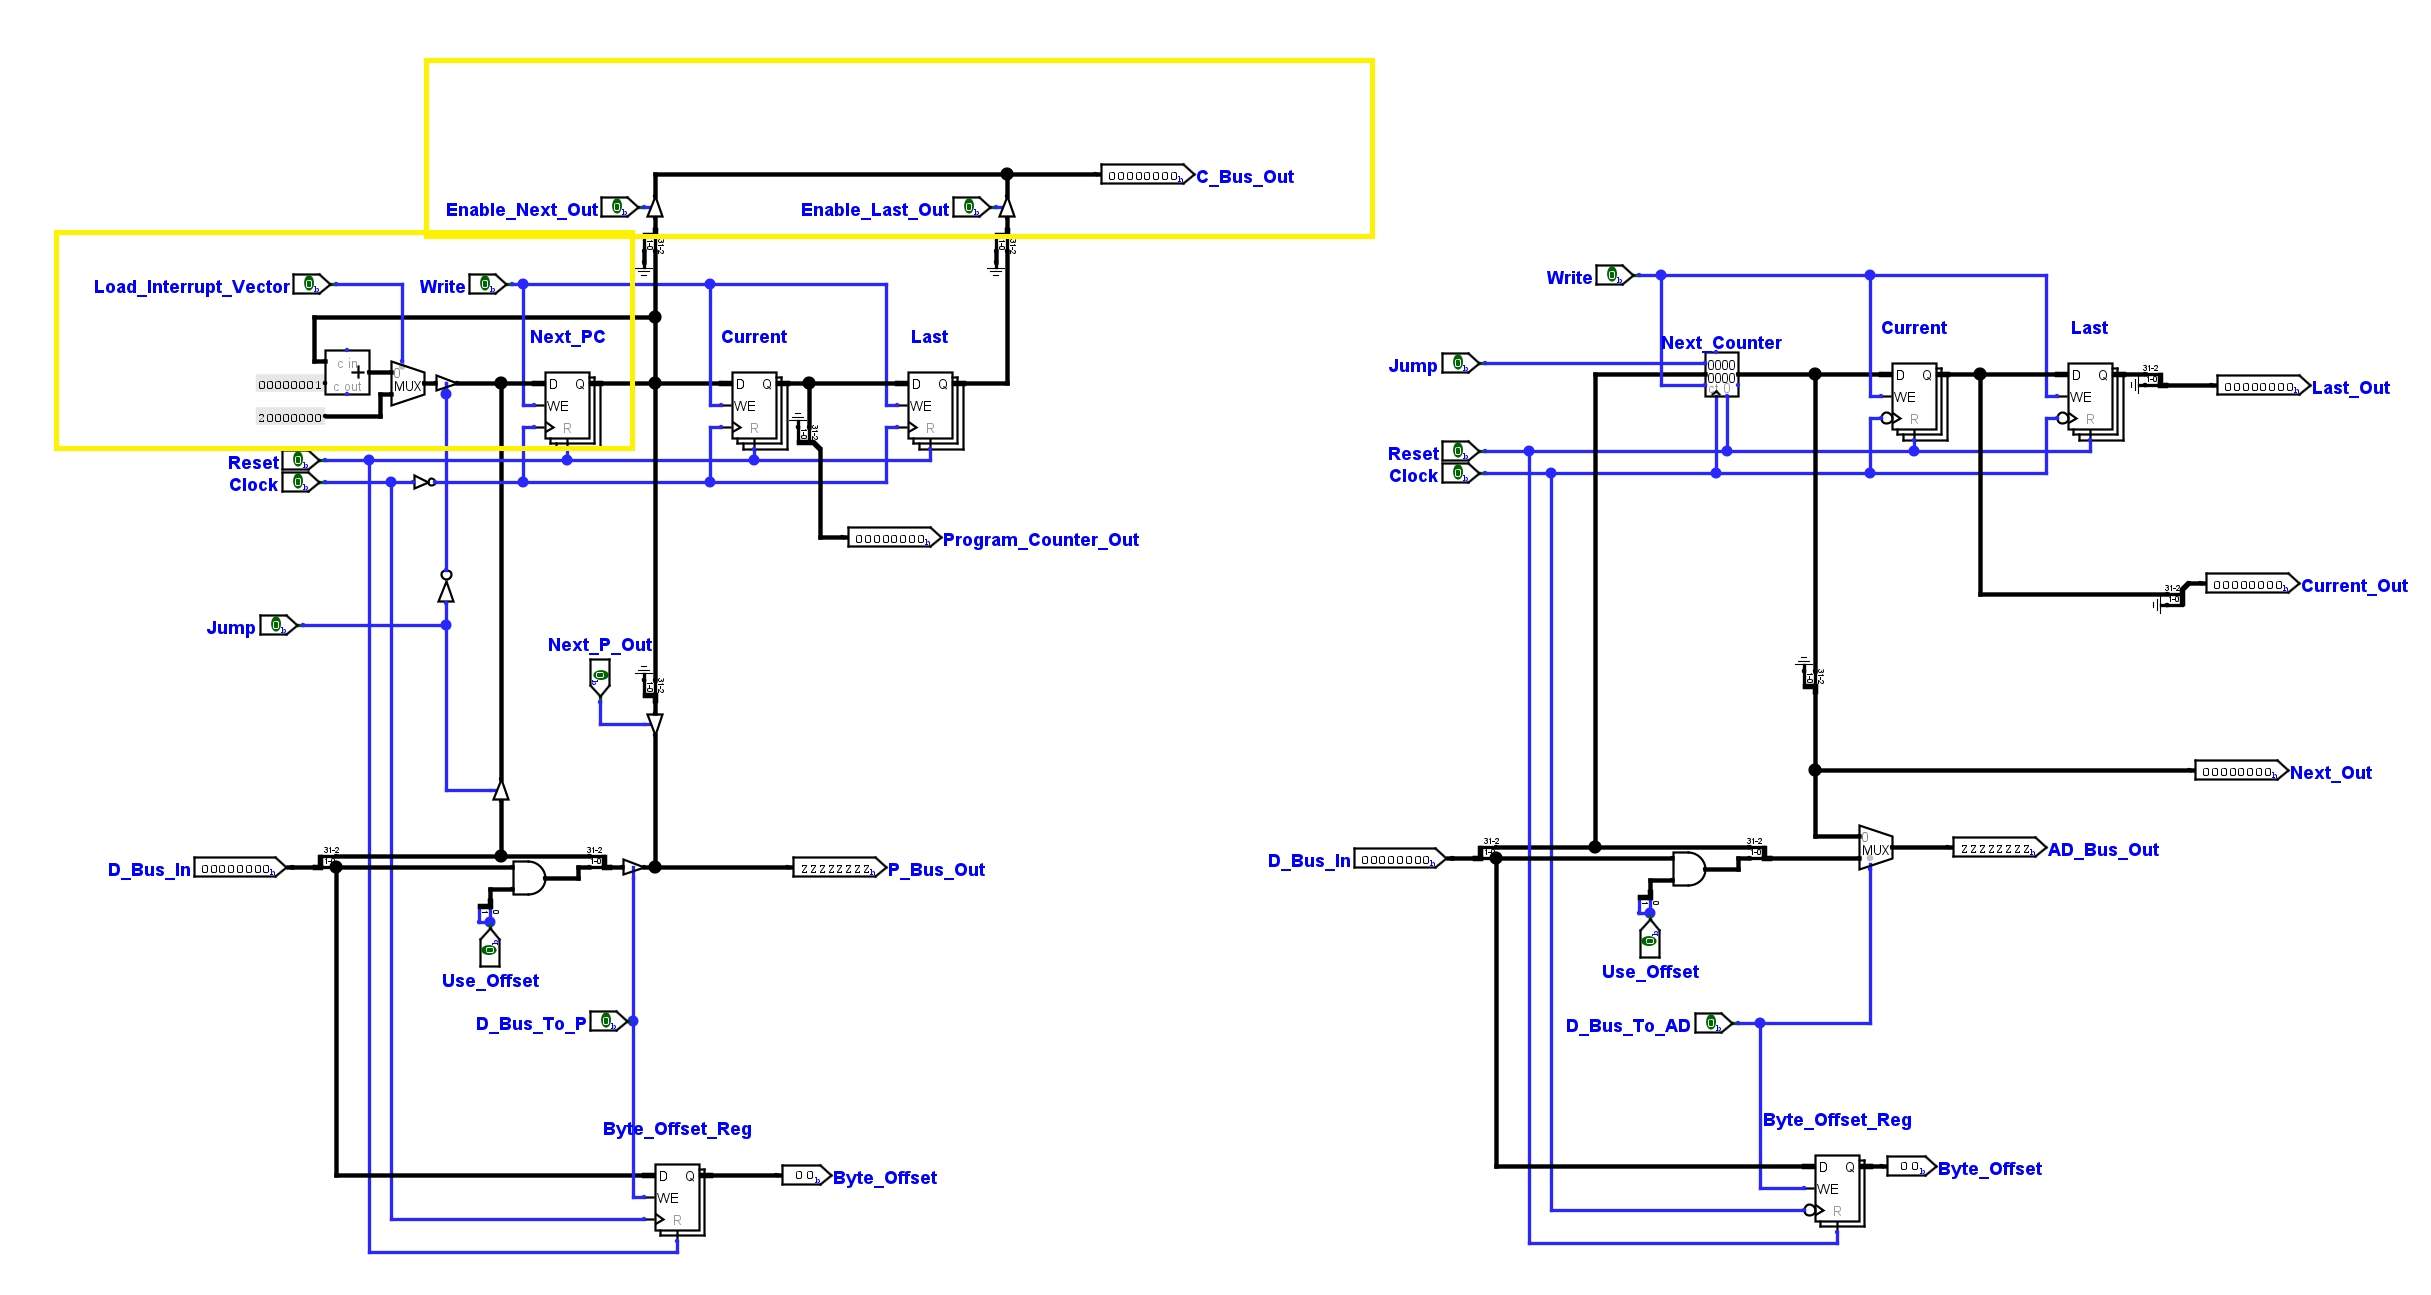
\includegraphics[width=0.8\linewidth]{ProcessoDesenvolvimento/Arquitetura/ContadorDePrograma1.png}
    \caption{Contador de Programa antes (esquerda) e depois (direita)}
    \label{fig:ContadorDePrograma1}
\end{figure}

Finalmente, durante essa etapa, os barramentos de endereço e dados foram separados (Figura~\ref{fig:barramentosSepara}), permitindo que dados e endereços sejam usados simultaneamente e evitando problemas na nova pipeline.

\begin{figure}[H]
    \centering
    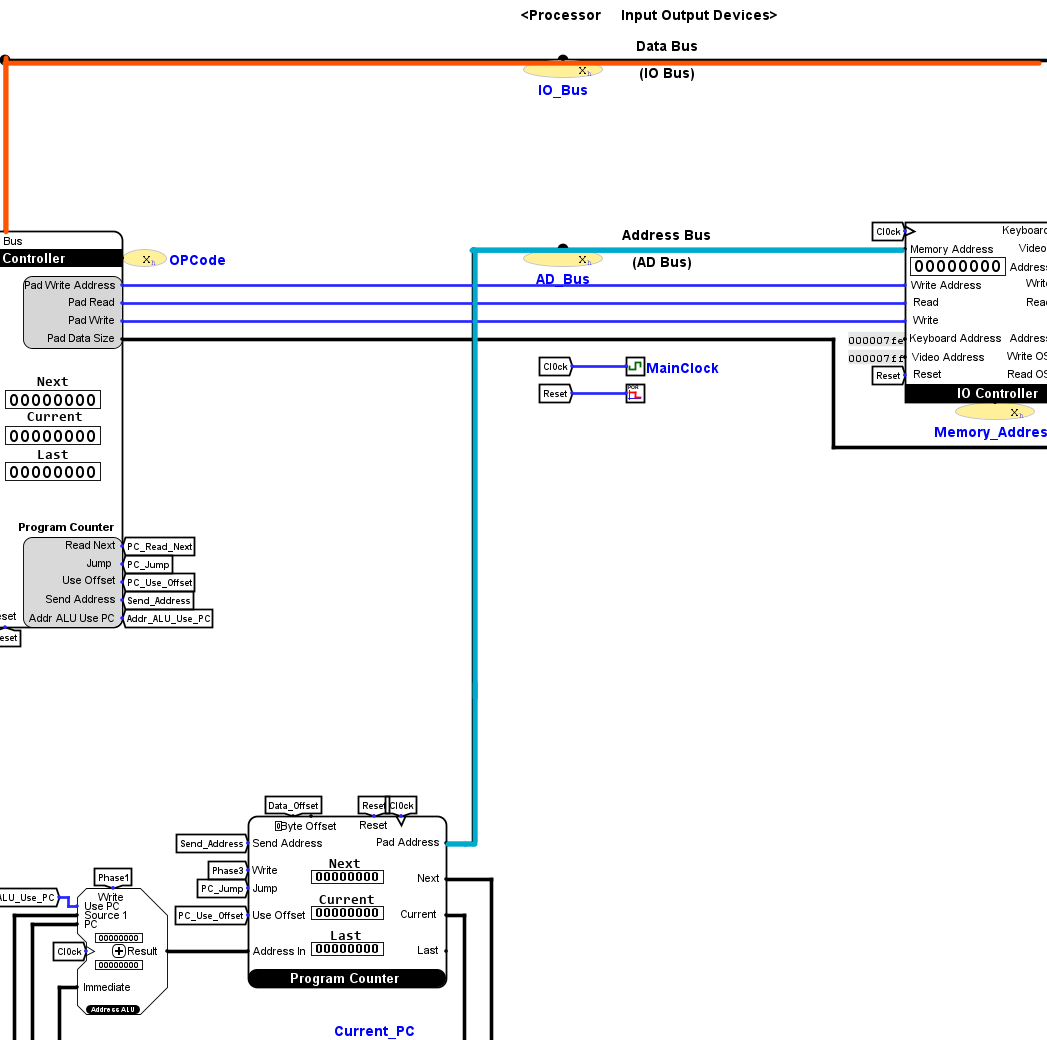
\includegraphics[width=0.8\linewidth]{ProcessoDesenvolvimento/Arquitetura/SeparacaoBarramentos.png}
    \caption{Separação dos barramentos de dados e endereços}
    \label{fig:barramentosSepara}
\end{figure}


\subsubsection{Terceira Fase: \textit{SystemVerilog}}

A terceira fase de desenvolvimento focou na conversão da arquitetura criada para uma especificação em uma linguagem de descrição de hardware (\ref{recursos_hdl}), especificamente o SystemVerilog (SV). O processo de conversão consistiu na tradução direta, componente por componente, da arquitetura. O resultado final possibilitou a criação de testes mais rápidos e robustos para a arquitetura, além de facilitar futuras alterações para uma interação mais rápida com o processador.

O primeiro componente a ser codificado foi a ULA, seguida pela ULA de Endereços, Contador de Programa, Arquivo de Registradores, Data IO, Controlador, o processador com todos os componentes anteriores e, finalmente, a memória RAM. Todo o código da primeira versão pode ser visto no Apêndice \ref{ap:arquitetura_sv_v1}.

Cada componente possuía um arquivo de teste individual, mas esses arquivos deixaram de ser utilizados após a criação do arquivo de teste principal, que integra o componente do processador à memória RAM e inclui código para imprimir o estado atual do sistema.

Para executar um programa via simulação no SV, os programas montados pelo \textit{assembler} são carregados na memória RAM através da rotina \$readmemh do SV. Essa rotina recebe o nome de um arquivo, que é lido e copiado para os registradores do componente. A formatação do arquivo é similar à dos arquivos criados pelo \textit{assembler}, mas é necessário remover os endereços e cabeçalhos.

Para permitir que o usuário troque o programa, o nome do arquivo pode ser passado como parâmetro durante a instanciação do componente no arquivo principal de testes. O arquivo principal também inclui parâmetros para controlar a largura do endereço de memória, o tamanho do programa em bytes, o tempo de oscilação do \textit{Clock}, o tempo limite de simulação e uma variável para selecionar uma das duas formas de impressão do estado do sistema.

A Figura~\ref{fig:sv_tests1} mostra o início da execução da simulação, utilizando a exibição simplificada do estado do processador. Nesta exibição, os valores são exibidos ao final de cada fase da \textit{Pipeline} (a cada 3 ciclos de \textit{Clock}), e informações sobre a instrução atual são apresentadas. Um processo simples de decompilação é executado para exibir os nomes legíveis da instrução e função atuais.

\begin{figure}[h]
    \centering
    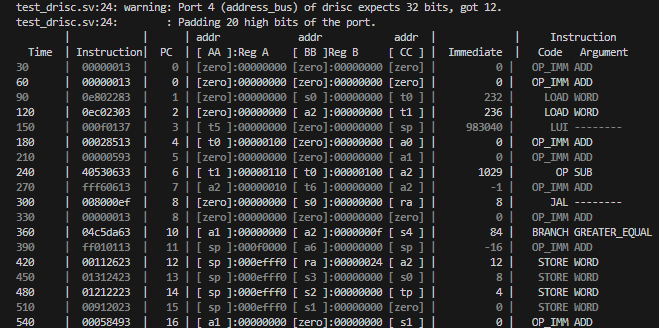
\includegraphics[width=0.75\linewidth]{ProcessoDesenvolvimento/Arquitetura/sv_tests1.png}
    \caption{Início da simulação do código SystemVerilog, com exibição simplificada do estado do sistema}
    \label{fig:sv_tests1}
\end{figure}

Embora essa simulação não seja interativa neste momento, ela ofereceu uma maneira alternativa de identificar erros no sistema. Ao intercalar a análise entre as simulações do Logisim Evolution e do Icarus Verilog, foi possível solucionar problemas que surgiam ao executar o algoritmo de ordenação \textit{quicksort}.

O fim da simulação pode ocorrer quando o tempo limite é alcançado, quando um salto para o próprio endereço é identificado ou quando uma instrução ilegal é detectada. Após isso, o conteúdo do Arquivo de Registradores e da Memória RAM é impresso, com destaque para os espaços de memória que sofreram alterações, como mostra a Figura~\ref{fig:sv_tests2}.

\begin{figure}[h]
    \centering
    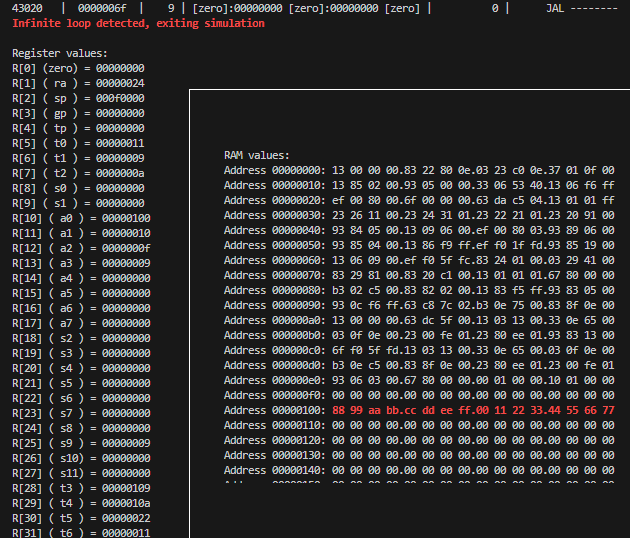
\includegraphics[width=0.75\linewidth]{ProcessoDesenvolvimento/Arquitetura/sv_testes2.png}
    \caption{Fim da simulação do código SystemVerilog}
    \label{fig:sv_tests2}
\end{figure}

Durante a criação do sistema, foi observado que a maioria das detecções de \textit{Clock} utilizadas para atualizar os registradores ocorria durante a borda de descida. A ideia inicial era que faria mais sentido enviar os dados durante a borda de subida do \textit{Clock} e escrevê-los durante a borda de descida. No entanto, após alguns testes, decidiu-se manter todas as ativações na borda de subida (\ref{recursos_padronizacao_sinais}), pois isso não alterava significativamente o funcionamento do sistema. Essa alteração de temporização também foi aplicada ao modelo de simulação no Logisim.

\begin{figure}[H]
    \centering
    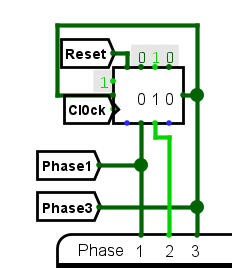
\includegraphics[width=0.25\linewidth]{ProcessoDesenvolvimento/Arquitetura/ContAnel.png}
    \caption{Contador em Anel, implementado com um Registrador de Deslocamento de 3 bits}
    \label{fig:cont_anel}
\end{figure}

Enquanto os sinais de ativação estavam sendo definidos, a entrada de fases do processador foi alterada para um gerador de fases interno. Esse gerador funciona com um contador em anel, que é atualizado durante a borda positiva do \textit{Clock}, conforme mostra a Figura~\ref{fig:cont_anel}.

Finalmente, durante essa fase, o sinal de \textit{overflow} calculado pela ULA foi alterado tanto no DRISC quanto no circuito do RISC~I. Esse sinal apresentava alguns problemas anteriormente, embora não afetasse o funcionamento de alguns programas de teste.

\subsubsection{Quarta Fase: Entrada e Saída}

Durante a replicação do RISC~I, alguns experimentos foram realizados para adicionar componentes que permitissem a interação do usuário. No entanto, esses experimentos se limitaram a testes simples, que não acrescentaram muito ao trabalho realizado. Nesta fase, um dos principais focos foi definir uma forma para permitir que os estudantes pudessem interagir com o sistema criado (\ref{recursos_melhoria_IO}).

No Logisim, alguns componentes foram escolhidos para permitir essa interação (Figura~\ref{fig:IO_Devices}), destacando-se o teclado e a tela. O teclado permite que o usuário digite caracteres, que são então transmitidos para sua saída com seus respectivos valores ASCII. A tela é um retângulo que, a partir de sinais de posição, cor e escrita, modifica seus pixels, permitindo a renderização de gráficos computados pelo processador.

\begin{figure}[h]
    \centering
    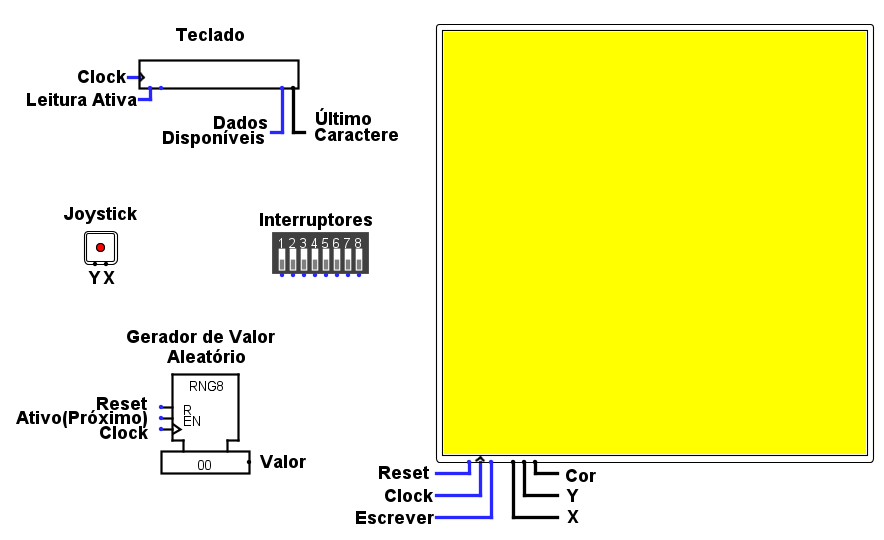
\includegraphics[width=0.75\linewidth]{ProcessoDesenvolvimento/Arquitetura/IO_Devices.png}
    \caption{Dispositivos de entrada e saída do Logisim utilizados}
    \label{fig:IO_Devices}
\end{figure}

Para conectar esses componentes ao processador, foi criado um componente que transmite os sinais de escrita e leitura caso o endereço atual esteja dentro de uma faixa de valores. Esse componente (Figura~\ref{fig:address_selector}) funciona como um controlador rudimentar de dispositivos de entrada e saída, ajudando a evitar conflitos no barramento de dados.

\begin{figure}[H]
    \centering
    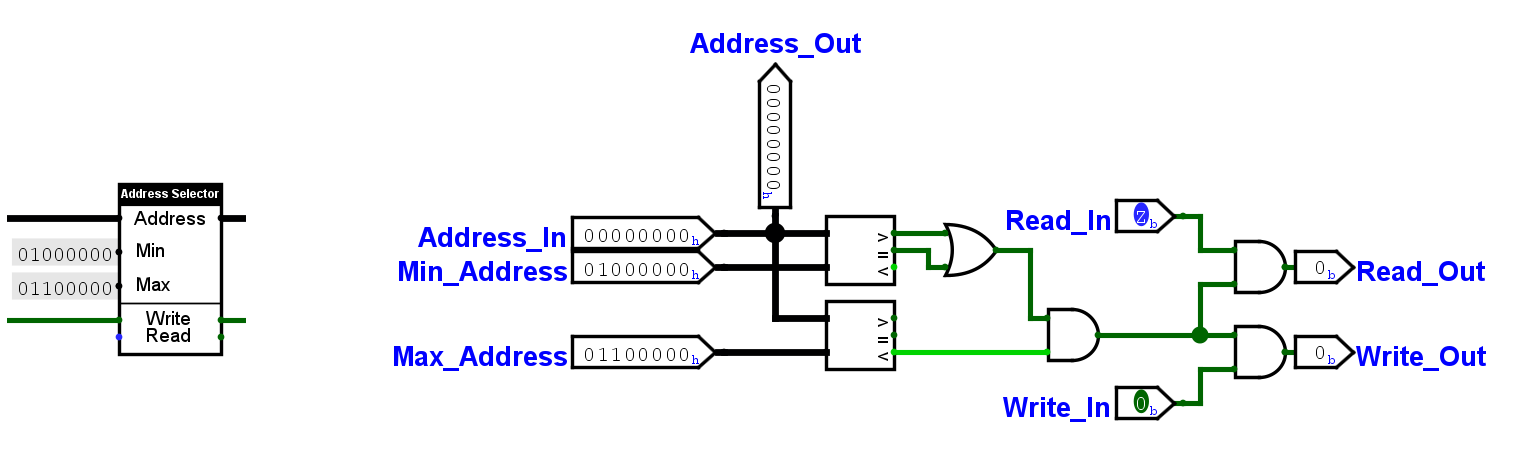
\includegraphics[width=0.75\linewidth]{ProcessoDesenvolvimento/Arquitetura/Address_Selector.png}
    \caption{Seletor de Endereços}
    \label{fig:address_selector}
\end{figure}

Com este novo componente, foram criadas alocações fixas para cada dispositivo de entrada e saída, conforme mostrado na Figura~\ref{fig:NewIOLogisim}. Considerando o último valor como exclusivo, a memória RAM ficou alocada entre os endereços \texttt{0x00000000} e \texttt{0x00fffffc}; um gerador de número aleatório, 8 interruptores, um \textit{joystick} e o teclado ficaram com os endereços \texttt{0x00fffffc} a \texttt{0x01000000}, e a tela com os endereços \texttt{0x01000000} a \texttt{0x01100000}.

\begin{figure}[h]
    \centering
    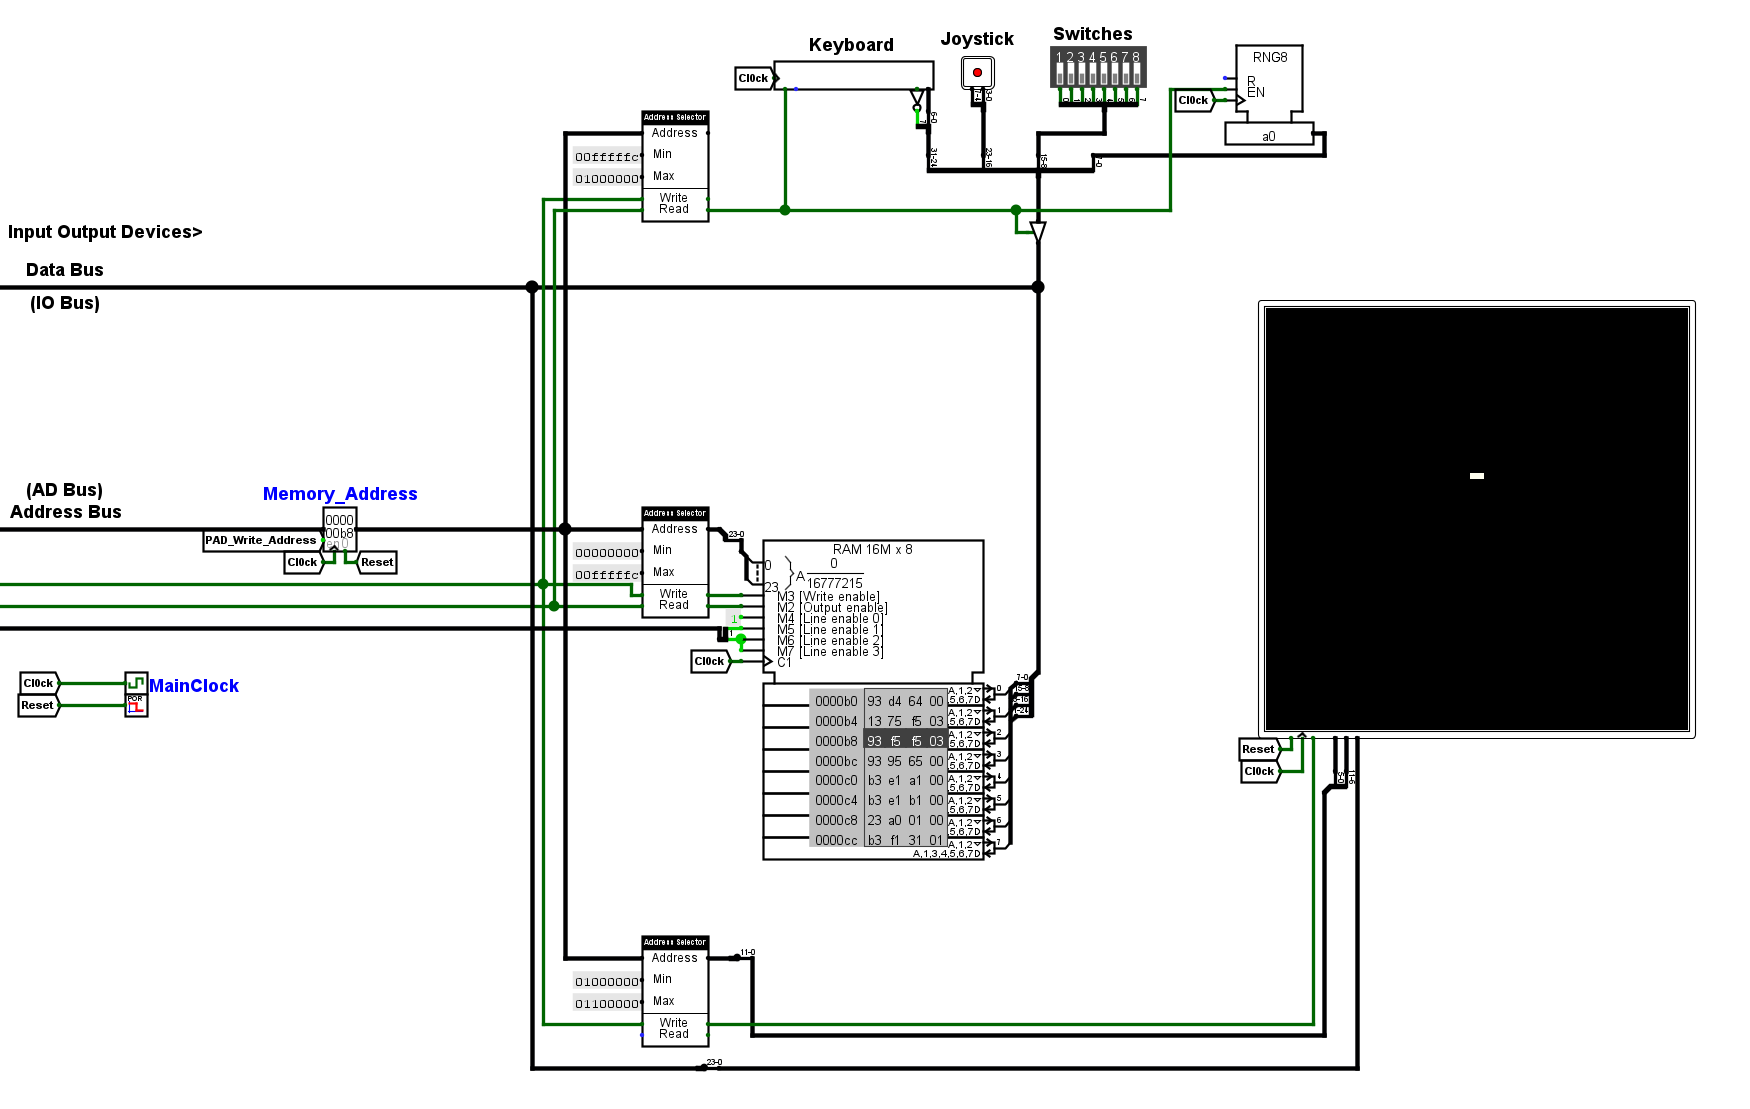
\includegraphics[width=1\linewidth]{ProcessoDesenvolvimento/Arquitetura/NewIOLogisim.png}
    \caption{Enter Caption}
    \label{fig:NewIOLogisim}
\end{figure}

Como cada dispositivo de entrada emite apenas um byte de informação, os 4 dispositivos de entrada foram colocados em uma palavra, o que permite o carregamento dos valores de todos os dispositivos simultaneamente ou o carregamento de um dos valores utilizando a instrução \texttt{lbu(load byte unsigned)}. Por exemplo, a partir do endereço \texttt{0x01000000} armazenado no registrador \texttt{gp}, podemos obter o valor do teclado com a instrução "\texttt{lbu~rd~gp~-1}" (carregar byte de [gp - 1] para o registrador \texttt{rd}), e o valor do \textit{joystick} com a instrução "\texttt{lbu~rd~gp~-2}" (carregar byte de [gp - 2] para o registrador \texttt{rd}).

Já a tela foi configurada de modo que cada pixel possuísse seu próprio endereço, com os 6 bits menos significativos representando a posição horizontal, enquanto os 6 bits subsequentes representam a posição vertical. Esse tamanho pode ser alterado para aumentar ou diminuir o tamanho da tela, porém, 6 bits por coordenada foram definidos como padrão por fins práticos. 

Ao escrever em qualquer um dos endereços da tela, o pixel correspondente troca para a cor que foi enviada, que deve estar no formato RGB~888(Em hexadecimal \texttt{0x00BBGGRR}). Outros formatos podem ser escolhidos, porém estes fornecem menos flexibilidade e não possuem alinhamento aos \textit{bytes} por canal de cor, o que pode dificultar o seu controle.

Para testar a entrada e saída, um programa simples para o DRISC foi desenvolvido (Apêndice~\ref{ap:testeIO}), onde um ponto em movimento é desenhado na tela e, utilizando as teclas W, A, S e D, o usuário pode modificar a direção desse ponto.

Após a definição das interfaces de entrada e saída, foi notado que os registradores presentes no Deslocador, na ULA e na ULA de endereços não eram necessários, isso porque os barramentos A e B contêm a informação necessária durante todo o ciclo de execução e escrita do arquivo de registradores.  

Essa remoção dos registradores também tirou a necessidade de um sistema de encaminhamento de dados (\ref{recursos_forward}), pois assim que o arquivo de registradores recebe os dados da memória, os dados atualizados não precisam ser repassados para os outros componentes.

Sem os registradores, a ULA de endereços e o Deslocador se tornaram muito simples para continuarem como componentes próprios, então o Deslocador foi fundido à ULA e a ULA de endereços foi fundida ao Contador de Programa. Os resultados dessas alterações podem ser vistos na Figura~\ref{fig:Shifter_removal}.
\begin{figure}
    \centering
    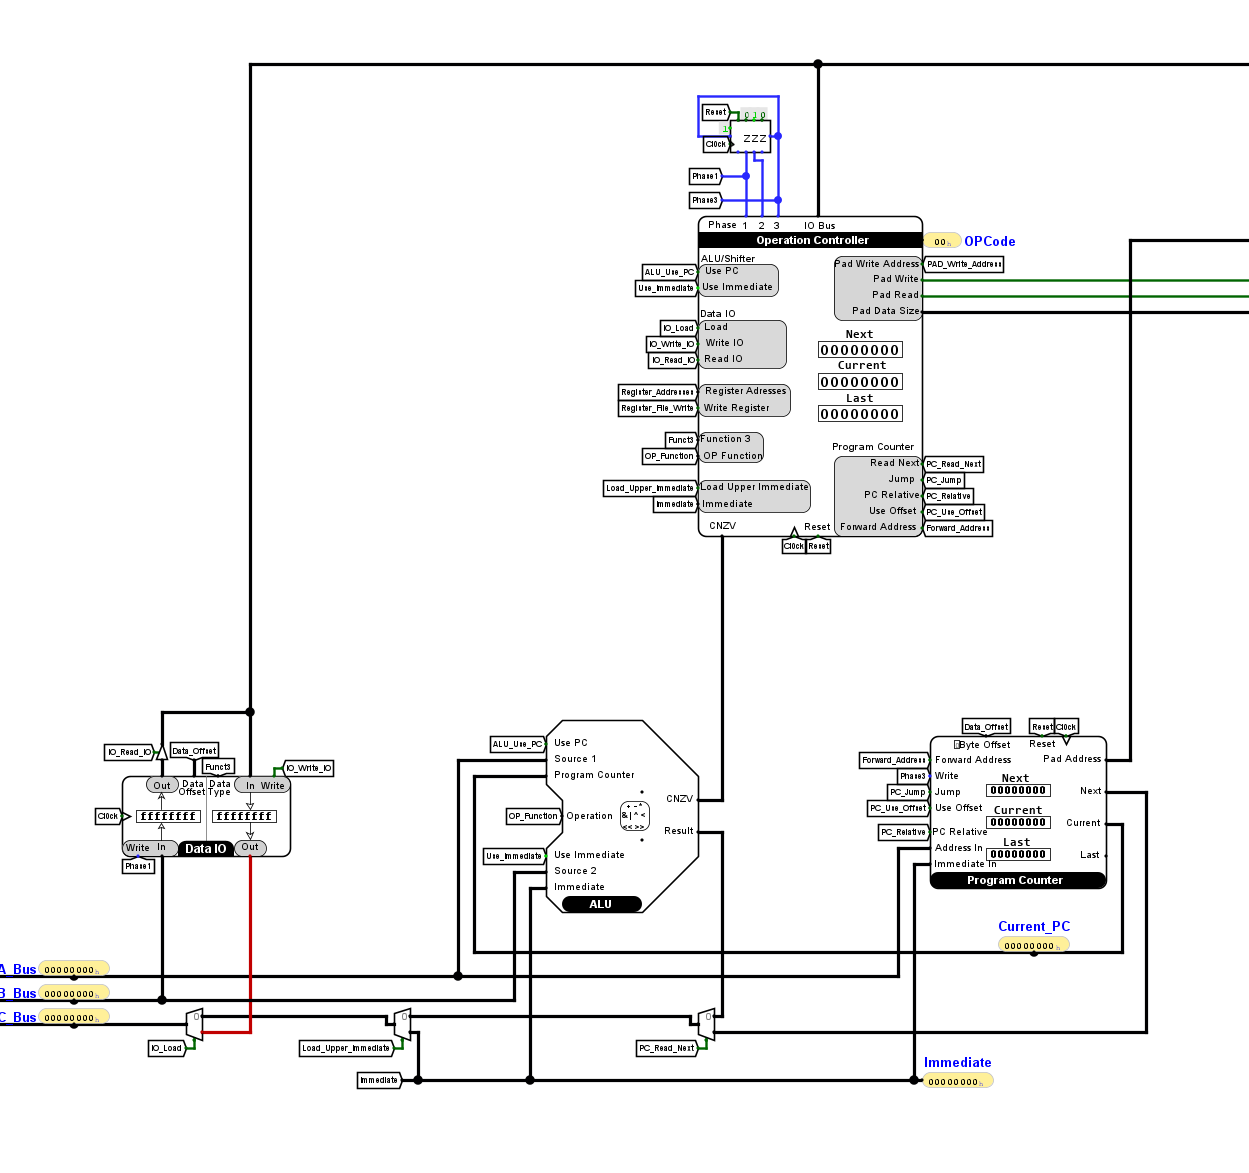
\includegraphics[width=1\linewidth]{ProcessoDesenvolvimento/Arquitetura/Shifter_removal.png}
    \caption{Resultado da remoção de registradores de entrada, do Deslocador e da ULA de endereços}
    \label{fig:Shifter_removal}
\end{figure}

Após essas alterações, as interfaces de entrada e saída foram implementadas no código SV, porém com alguns desafios. O maior deles foi que simuladores como o Icarus Verilog não oferecem uma forma fácil de interação em tempo real com a simulação. Para contornar isso, algumas opções foram analisadas, como a compilação do código utilizando o Verilator ou o recurso DPI (Interface de Programação Direta) do SystemVerilog.

O Verilator \cite{snyder_verilator_2003} é um programa que transforma código Verilog ou SystemVerilog em código C++ ou SystemC para simulação. Ele verifica o código, faz checagens de erros e pode adicionar pontos de análise. O resultado é um conjunto de arquivos que podem ser compilados para criar um modelo simulável. Esse modelo permite testar e simular o design do hardware, integrando-o com código C customizado.

Apesar de sua proposta promissora, o Verilator possui uma grande limitação: a falta de suporte para sistemas operacionais Windows. Soluções para isso envolveriam compilar o Verilator manualmente ou utilizar máquinas virtuais. No entanto, como o objetivo é obter um ambiente didático fácil de ser utilizado, essa solução foi descartada por ser muito complexa.

O recurso DPI, por outro lado, oferece uma forma de comunicação direta com códigos escritos em C. Esses códigos devem ser compilados como bibliotecas que são anexadas à simulação. Funções criadas no código SV e no código C são exportadas de um lado e importadas pelo outro. Isso permitiria, por exemplo, que uma função no lado do SV criasse um aplicativo com uma interface gráfica no lado do C. Esse tipo de integração poderia ser facilmente utilizado, mas o Icarus Verilog não possui suporte para o recurso DPI.

Uma última solução foi encontrada, utilizando funções do SystemVerilog para ler e modificar arquivos. Esses arquivos podem então ser utilizados como uma interface entre a simulação e outros programas. Apesar dessa solução possuir vários pontos negativos, ela ainda é simples o suficiente para não precisar de uma configuração complexa.

O primeiro componente a ser codificado foi a tela (Disponível no Apêndice \ref{ap:arquitetura_sv_v1}). O funcionamento base desse componente é similar a uma memória RAM sem função de leitura, ou seja, o componente possui apenas entradas que permitem a escrita no seu conjunto de registradores. Esse conjunto é então periodicamente copiado para o arquivo externo, caso modificações tenham sido feitas na memória.

Após a criação do componente de tela, desenvolveu-se um novo programa em C\#, responsável pela leitura dos dados da tela, como ilustrado na Figura~\ref{fig:DRISC-V_interface}. Cada número presente no arquivo de tela é interpretado como um pixel pelo programa, gerando o mesmo resultado visual observado na simulação com o Logisim.

\begin{figure}[h]
    \centering
    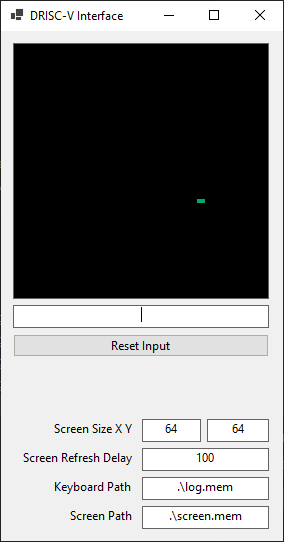
\includegraphics[width=0.25\linewidth]{ProcessoDesenvolvimento/Arquitetura/DriscV_Interface.png}
    \caption{Programa para interação com a simulação SV, denominado DRISC-V Interface}
    \label{fig:DRISC-V_interface}
\end{figure}

Foi incorporada também uma entrada para teclado, onde cada caractere digitado é convertido em um número hexadecimal e adicionado ao final do arquivo de entrada. Um componente de entrada na simulação acessa esse arquivo a cada sinal de leitura. Outros tipos de entrada ainda não foram implementados, com exceção do gerador de números aleatórios, o qual foi codificado diretamente no componente de entrada.

Na primeira versão do \textit{DRISC-V Interface}, era possível configurar parâmetros como o tamanho da tela, a frequência de leitura do arquivo de tela e os nomes dos arquivos de entrada e saída.

Já nas etapas finais do desenvolvimento, adicionou-se um novo dispositivo de saída: o Terminal. Esse componente foi projetado para a impressão rápida de texto, evitando a necessidade de renderizar individualmente cada caractere durante a exibição de informações.

No Logisim, o terminal possui uma entrada de 7 bits, permitindo a impressão de qualquer caractere da tabela ASCII, além de um sinal adicional para limpeza do conteúdo. Os endereços designados para o terminal foram \texttt{0x01100000} para escrita e \texttt{0x01100001} para limpeza.

No código da simulação SV, a implementação do terminal seguiu um conceito semelhante ao da tela. Contudo, em vez de um valor de pixel por linha, o arquivo final contém uma lista de bytes correspondentes ao buffer de dados do terminal. Esses dados são interpretados pela interface, que foi atualizada conforme mostrado na Figura~\ref{fig:DRISC-V_interface_Final}.

\begin{figure}[h]
    \centering
    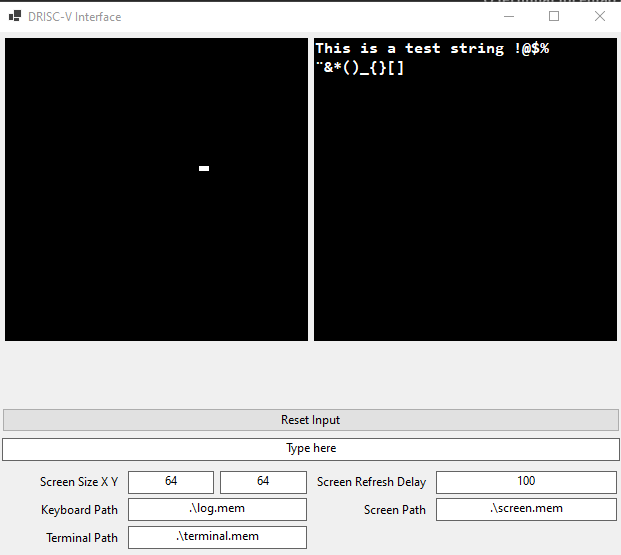
\includegraphics[width=0.75\linewidth]{LastSVInterface.png}
    \caption{Interface atualizada para interação com os dados do terminal}
    \label{fig:DRISC-V_interface_Final}
\end{figure}

\subsubsection{Quinta Fase: Controlador de Registradores de Controle e Status }

Com a base dos dispositivos de E/S prontos, foi decidida a adição de um novo sistema de interrupções(\ref{recursos_interrupt}). O sistema antigo do RISC~I havia sido removido por não possuir mais funções válidas na nova versão do processador; porém, o RISC-V possui uma especificação sobre exceções e interrupções que puderam ser implementadas, presente no volume II do manual de especificação \citeonline{risc-v_risc-v_2024-1}.

Para atender à especificação, a expansão \textit{Zicsr} de registradores de controle e estado(CSRs) teve de ser implementada. Essa expansão adiciona registradores fundamentais para o tratamento de interrupções, além de ser requerida pela arquitetura privilegiada do \citeonline{risc-v_risc-v_2024-1}, podendo ser aproveitada para a implementação dos modos de Máquina(Kernel) e Usuário (\ref{recursos_kernel}). 

Durante a implementação da expansão Zicsr foram implementadas atualizações no funcionamento da pipeline. A primeira modificação envolveu a redefinição do momento de atualização dos registradores referentes à instrução atual e à última instrução. Originalmente, essa atualização era realizada na borda de descida do \textit{clock}, o que gerava uma assincronia entre a fase e os registradores. Esse descompasso dificultava a análise e compreensão dos eventos, além de aumentar a propensão a erros de sincronismo durante o desenvolvimento.

\begin{figure}[h]
    \centering
    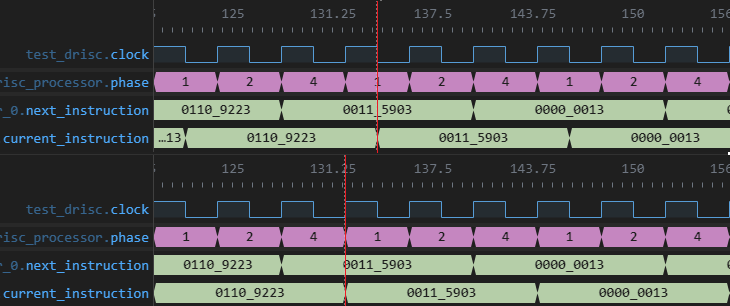
\includegraphics[width=0.75\linewidth]{ProcessoDesenvolvimento/Arquitetura/NovoTiming_1.png}
    \caption{Alteração no momento de atualização do registrador de instrução atual (\textit{current\_instruction})}
    \label{fig:current_inst_sync}
\end{figure}

Para corrigir esse problema, o momento de atualização dos registradores foi alterado: em vez de ocorrer na borda de descida do \textit{clock} durante a fase 1, passou a ser realizado na borda de subida durante a fase 3. O resultado dessa modificação pode ser observado na Figura~\ref{fig:current_inst_sync}. É importante destacar que, como a atualização dos registradores depende da fase, e a fase é influenciada pelo \textit{clock}, a fase utilizada deve preceder a subida do \textit{clock}. Por esse motivo, a fase escolhida é a 3, e não a 1.

A segunda alteração, porém,  foi de maior impacto: a remoção de uma das fases da pipeline. Essa remoção  não só simplificou a execução das instruções, mas também envolveu a remoção de registradores e a simplificação de circuitos de controle, além de um aumento efetivo de cerca de 33\% no tempo de processamento de instruções.

A ideia sobre essa alteração foi que, após todas as mudanças feitas até esse momento na arquitetura, diversos espaços ficaram livres entre as fases da pipeline, tornando a execução desnecessariamente mais demorada. Com isso em mente, foram analisados os possíveis conflitos entre os sinais durante cada parte da pipeline, e todos os sinais foram movidos para a primeira fase possível, resultando na \textit{Pipeline} vista na Tabela \ref{tab:2phase3parts_pipeline}. 

\begin{table}[h!]
\centering
\resizebox{\textwidth}{!}{%
\begin{tabular}{|>{\centering\arraybackslash}m{2cm}|>{\centering\arraybackslash}m{3.5cm}|>{\centering\arraybackslash}m{9cm}|>{\centering\arraybackslash}m{9cm}|}
\hline
\textbf{Passo Da Pipeline} & \textbf{Instrução/Passo} & \textbf{Fase 1} & \textbf{Fase 2} \\ \hline \hline
\multirow{2}{*}{1} & \multirow{2}{*}{\makecell{Coleta de Instrução \\ e Decodificação}} & \multirow{2}{*}{RAM $\rightarrow$ Próxima Instrução} & Próxima Instrução $\rightarrow$ Instrução Atual \\ 
  &                                     &                                      & Endereço da Próxima Instrução $\rightarrow$ Barramento de Endereços \\ \hline \hline
\multirow{5}{*}{2}  & Todas Instruções   &                                      & Resultado $\rightarrow$ Arquivo de Registradores \\ \cline{2-4}
  & Load                                & Endereço do dado $\rightarrow$ Barramento de Endereços & Dispositivo de E/S $\rightarrow$ DataIO \\ \cline{2-4}
  & Store                               &                                      & DataIO $\rightarrow$ Dispositivo de E/S \\ \cline{2-4}
  & Jump                                &                                      & Endereço do Pulo $\rightarrow$ Próximo PC \\ \cline{2-4}
  & Branch                              &                                      & Se verdade: Endereço do Pulo $\rightarrow$ Próximo PC \\ \hline \hline
3 & Load                                & Resultado $\rightarrow$ Arquivo de Registradores & \\ \hline
\end{tabular}
}
\caption{Nova \textit{Pipeline} de 3 passos e 2 fases}
\label{tab:2phase3parts_pipeline}
\end{table}

Nessa nova pipeline, a instrução de \texttt{store} é executada durante 2 passos, contrário aos 3 passos que utilizava anteriormente; porém, a instrução de \texttt(load) foi mantida durante o terceiro passo como uma forma de lidar com atrasos de leitura de informação da memória, mesmo que este caso não aconteça durante a simulação. 

O aumento de velocidade se deve ao fato de que uma nova instrução é processada a cada 2 ciclos de \textit{clock}, ao invés dos 3 ciclos anteriores, e foi verificado a partir da cronometragem da execução do programa de entrada e saída, onde o tempo de escrita de uma linha na tela foi de 4 segundos para em torno de 2,67 segundos.

Com essas alterações sobre a pipeline, o Controlador de CSRs pôde ser construído. Diferentemente dos outros componentes, este foi inicialmente criado através do código SV. Isso foi feito pois este componente possui um certo nível de complexidade no seu comportamento que é melhor expresso por código, além de que os testes sobre o código são mais simples de serem executados.

O primeiro passo para a criação desse controlador foi a escolha de quais CSRs seriam utilizados. Para isso, a especificação privada do \citeonline{risc-v_risc-v_2024-1} foi consultada. Alguns dos CSRs são obrigatórios para a implementação, como o \texttt{mvendorid}, que contém um identificador JEDEC do fabricante do processador; porém, no nosso caso, podemos apenas colocar valores de exemplo nesses registradores. 

A Tabela \ref{tab:registers} mostra todos os CSRs que foram implementados na arquitetura:
{\fontsize{11}{13}\selectfont
\begin{longtable}{|p{3cm}|p{5cm}|p{8cm}|}
\hline  
\textbf{Nome} & \textbf{Resumo} & \textbf{Notas} \\ 
\hline  
M VENDOR ID & Identifica o fabricante & Valor fixo 0x00af001d \\ 
\hline  
M ARCH ID & Identifica a arquitetura & Valor fixo 0x00000000 \\ 
\hline  
M IMP ID & Identifica a implementação & Valor fixo para cada atualização da arquitetura. \\ 
\hline  
M HART ID & ID do núcleo de hardware & Valor fixo 0x00000000 (núcleo único) \\ 
\hline  
M STATUS & Contém alguns bits relacionados ao estado do processador & Bits que foram implementados: Privilégio Anterior (PP), Interrupção Ativa (IE) e Interrupção Ativa Anterior (PIE) \\ 
\hline  
M ISA & Indica as expansões disponíveis e ativas do processador & Não foi implementada uma forma de desativar expansões. As expansões implementadas foram E, I, M (sem divisão) e U \\ 
\hline  
M I E & Bits que permitem a ativação de interrupções & Apenas foram implementadas interrupções de \textit{software}, \textit{timer} e externas a nível de máquina. \\ 
\hline  
M T VEC & Registrador que contém o endereço com tratamento de interrupções e exceções & O valor padrão é 0x80000001, o que significa que o endereço base é 0x80000000 e cada tipo de interrupção é levado para um endereço diferente \\ 
\hline  
M STATUS H & Bits superiores do M STATUS & O único bit que contém informação relevante é o de endianismo do modo usuário, que é fixo em 0 nessa implementação. \\ 
\hline  
M SCRATCH & Registro temporário & Usado para armazenamento temporário de informações durante o tratamento de \textit{traps}. \\ 
\hline  
M E PC & Contador de programa de exceção & Indica o último endereço de memória acessado antes de uma \textit{trap}. \\ 
\hline  
M CAUSE & Causa da \textit{trap} & Além das interrupções, a causa também pode ser relacionada a algumas exceções, como as de endereços desalinhados ou instruções ilegais. \\ 
\hline  
M T VAL & Valor da \textit{trap} & Contém o valor que causou a \textit{trap}, podendo ser uma instrução ou um endereço calculado. \\ 
\hline  
M I P & Interrupção pendente & O seu valor é controlado por sinais de dispositivos externos ao processador, e seus bits são equivalentes aos bits do MIE \\ 
\hline  
CYCLE & Contador de ciclos & Um contador que atualiza a cada ciclo de \textit{clock}. Cada fase da \textit{Pipeline} dura dois ciclos de \textit{clock}. \\ 
\hline  
TIME & Contador de tempo & Ao ser lido, ativa uma instrução de carregamento de um registrador endereçado na memória. \\ 
\hline  
INST RET & Contador de instruções executadas & Incrementa por instrução iniciada a cada dois ciclos de clock. Não incrementa durante exceções. \\ 
\hline  
CYCLE H & Bits superiores do CYCLE & -- \\ 
\hline  
TIME H & Bits superiores do TIME & -- \\ 
\hline  
INSTRET H & Bits superiores do INSTRET & -- \\ \hline  
\captionsetup{width=1\textwidth}
\caption{Registradores de Controle e Estado implementados na arquitetura.}
\label{tab:registers}
\end{longtable}
}
Após a escolha e o estudo detalhado das especificações dos registradores, sua implementação foi realizada de forma individual, atendendo aos requisitos técnicos necessários.

Inicialmente, o foco esteve na implementação das instruções responsáveis pela manipulação dos registradores. Essas instruções realizam a leitura de um CSR-alvo enquanto simultaneamente modificam seu conteúdo por meio de uma das três operações disponíveis: escrita, definição ou limpeza. A lógica geral para a implementação dessas instruções está descrita nos Algoritmos \ref{alg:rotina_sincrona} e \ref{alg:novo_valor_calculado}.

\begin{algorithm}[h!]
\caption{Rotina Síncrona do Controlador de CSR}
\label{alg:rotina_sincrona}
\begin{algorithmic}[1]
    \IF{é reset}
        \STATE Inicializar os registradores com os valores iniciais
    \ELSIF{é fase 2}
        \IF{é Interrupção \textbf{OU} Exceção}
            \STATE Executar rotina de \textit{trap}
        \ELSIF{é instrução MRET}
            \STATE Executar rotina do MRET
        \ELSIF{\textcolor{blue}{é instrução de manipulação de CSR \textbf{E} CSR é válido}}
            \STATE \textcolor{blue}{CSR selecionado $\leftarrow$ \texttt{NovoValorCalculado()}}
        \ENDIF

        \IF{\textbf{NÃO} é Exceção}
            \STATE Incrementar contador INSTRET: INSTRET $\leftarrow$ INSTRET + 1
        \ENDIF
    \ELSIF{\textcolor{blue}{é fase 1 \textbf{E} é instrução de manipulação de CSR \textbf{E} CSR é válido}}
        \STATE \textcolor{blue}{Barramento C $\leftarrow$ valor do registrador selecionado}
    \ENDIF

    \IF{\textbf{NÃO} é reset}
        \STATE Incrementar contador CYCLE: CYCLE $\leftarrow$ CYCLE + 1
    \ENDIF
\end{algorithmic}
\end{algorithm}

O Algoritmo \ref{alg:rotina_sincrona} ilustra como as instruções são implementadas na rotina síncrona do CSR, que é executada em cada borda de subida do \textit{clock}. Este processo garante a operação correta dos registradores e suas interações com as instruções associadas. Tentativas de escrita para CRSs que só permitem leitura são ignoradas; porém, tentativas de leitura ou escrita de CSRs que exigem um nível de operação superior ao que está sendo utilizado emitem um sinal de CSR ilegal e não são executadas.

Já o Algoritmo \ref{alg:novo_valor_calculado} apresenta a lógica utilizada para calcular o novo valor que será gravado nos CSRs durante a execução das instruções de manipulação.

\begin{algorithm}[h!]
\caption{Função NovoValorCalculado()}
\label{alg:novo_valor_calculado}
\begin{algorithmic}[1]
    \REQUIRE Registrador, Dado
    \ENSURE Novo valor do CSR
    \IF{modo de operação é escrita}
        \RETURN Dado
    \ELSIF{modo de operação é definição}
        \RETURN Registrador \textbf{OU} Dado
    \ELSIF{modo de operação é limpeza}
        \RETURN Registrador \textbf{E NÃO} Dado
    \ELSE
        \RETURN \textit{nenhum valor}
    \ENDIF
\end{algorithmic}
\end{algorithm}

Com a manipulação dos CSRs devidamente implementada, o próximo passo foi a integração das funcionalidades de Exceções e Interrupções. Para isso, foram criados os seguintes sinais:

\begin{itemize}
    \item \textbf{Interrupção:} Indica a ocorrência de uma interrupção.
    \item \textbf{Exceção:} Indica a ocorrência de uma exceção.
    \item \textbf{Causa (da \textit{trap}):} Contém a causa da interrupção ou exceção.
    \item \textbf{Valor (da \textit{trap}):} Armazena dados adicionais utilizados no tratamento de determinadas exceções.
\end{itemize}

Esses sinais são gerenciados de forma assíncrona por meio do decodificador, cuja lógica está detalhada no Algoritmo \ref{alg:rotina_assincrona}. 

\begin{algorithm}[h!]
\caption{Rotina Assíncrona do Controlador de CSR}
\label{alg:rotina_assincrona}
\begin{algorithmic}[1]
    \STATE \textbf{Inicialização dos Sinais Assíncronos:}
    \STATE \hspace{1em} Interrupção $\leftarrow$ \FALSE
    \STATE \hspace{1em} Exceção $\leftarrow$ \FALSE
    \STATE \hspace{1em} Causa $\leftarrow$ Nenhuma
    \STATE \hspace{1em} Valor $\leftarrow$ 0
    \STATE
    \IF{interrupções estão ativas \textbf{OU} é \textbf{Modo Usuário}}
        \IF{interrupção \textit{X} está ativa \textbf{E} pendente}
            \STATE Interrupção $\leftarrow$ \TRUE
            \STATE Causa $\leftarrow$ Interrupção \textit{X}
        \ENDIF
    \ENDIF
    \STATE
    \IF{Interrupção = \TRUE}
        \IF{MTVEC está no modo vetorizado}
            \STATE Endereço Alvo $\leftarrow$ MTVEC + (Causa $\times$ 4)
        \ELSE
            \STATE Endereço Alvo $\leftarrow$ MTVEC
        \ENDIF
    \ELSIF{Alguma condição para exceção é \TRUE}
        \STATE Exceção $\leftarrow$ \TRUE
        \STATE Causa $\leftarrow$ Código da exceção
        \STATE Valor $\leftarrow$ Instrução Atual, Endereço Calculado ou 0
    \ELSIF{é uma instrução MRET}
        \STATE Endereço Alvo $\leftarrow$ MEPC
    \ENDIF
    \STATE
    \IF{Exceção = \TRUE}
        \STATE Endereço Alvo $\leftarrow$ MTVEC
    \ENDIF
\end{algorithmic}
\end{algorithm}

É importante destacar que há uma ordem de prioridade codificada conforme especificado por \citeonline{risc-v_risc-v_2024-1}. Essa ordem segue o seguinte esquema:
\begin{enumerate}
    \item \textbf{Interrupções:}
    \begin{enumerate}
        \item Externa (prioridade mais alta).
        \item Software.
        \item Timer.
    \end{enumerate}
    \item \textbf{Exceções:}
    \begin{enumerate}
        \item Instrução Ilegal.
        \item Endereço de Instrução Desalinhado.
        \item Breakpoint.
        \item ECALL a partir do Modo Máquina.
        \item ECALL a partir do Modo Usuário.
        \item Endereço de Carregamento Desalinhado.
        \item Endereço de Salvamento Desalinhado.
    \end{enumerate}
\end{enumerate}
Vale observar que alguns eventos possuem a mesma prioridade ou não podem ocorrer simultaneamente.

Os sinais são então utilizados durante a rotina de execução das \textit{traps}, bem como na gravação dos CSRs relacionados, conforme apresentado no Algoritmo \ref{alg:rotina_trap}. Esta rotina faz parte da execução síncrona detalhada anteriormente no Algoritmo \ref{alg:rotina_sincrona}. 

\begin{algorithm}[h!]
\caption{Rotina de \textit{Trap} (Porção Síncrona)}
\label{alg:rotina_trap}
\begin{algorithmic}[1]
    \STATE Interrupção Ativa Anterior $\leftarrow$ Interrupção Ativa
    \STATE Interrupção Ativa $\leftarrow$ \FALSE
    \STATE Privilégio Anterior $\leftarrow$ Privilégio
    \STATE Privilégio $\leftarrow$ \textbf{Modo Máquina (Kernel)}
    \STATE MEPC $\leftarrow$ Contador de Programa Atual
    \STATE MCAUSE $\leftarrow$ Causa (da \textit{trap})
    \STATE MTVAL $\leftarrow$ Valor (da \textit{trap})
\end{algorithmic}
\end{algorithm}

Inicialmente, a rotina foca em desativar as interrupções para evitar que novas \textit{traps} sejam acionadas enquanto as interrupções pendentes estão sendo tratadas. Além disso, o Modo Máquina é ativado, permitindo que o sistema em execução acesse recursos privilegiados, como CSRs específicos que são essenciais para o tratamento de exceções e interrupções.

Ao final da rotina, o contador de programa é salvo no CSR MEPC, garantindo que o retorno ao programa ocorra após o término do tratamento da exceção ou interrupção. Além disso, os CSRs responsáveis por armazenar a causa e o valor da \textit{trap} são atualizados, proporcionando informações essenciais para o processamento dessas situações no nível de sistema.

Para retornar aos programas após uma rotina de tratamento, a instrução MRET deve ser executada. Essa instrução permite o retorno ao privilégio anterior e reativa as interrupções previamente habilitadas. Além disso, ela faz com que o contador de programa salte para o endereço que estava sendo executado antes da rotina de tratamento. A porção síncrona da MRET está detalhada no Algoritmo \ref{alg:rotina_mret}, enquanto a parte assíncrona, apresentada no Algoritmo \ref{alg:rotina_assincrona}, é responsável por atribuir o endereço de retorno ao sinal Endereço Alvo.

\begin{algorithm}[h!]
\caption{Rotina do MRET (\textit{Machine Return}) (Porção Síncrona)}
\label{alg:rotina_mret}
\begin{algorithmic}[1]
    \STATE Interrupção Ativa $\leftarrow$ Interrupção Ativa Anterior
    \STATE Interrupção Ativa Anterior $\leftarrow$ \TRUE
    \STATE Privilégio $\leftarrow$ Privilégio Anterior
    \STATE Privilégio Anterior $\leftarrow$ \textbf{Modo Usuário}
\end{algorithmic}
\end{algorithm}

O sinal Endereço Alvo é um dos principais sinais da interface do controlador. Ele é transmitido ao Contador de Programa, onde pode ser utilizado como endereço de pulo ou endereço de carregamento. Para viabilizar o uso do Endereço Alvo no Contador de Programa, foram criados dois sinais adicionais: o Pulo de Sistema (\textit{System\_Jump}) e o Carregamento de Sistema (\textit{System\_Load}).

O Pulo de Sistema funciona de maneira semelhante ao sinal de pulo do Controlador de Operações, mas possui prioridade mais alta. Isso significa que, caso ambos os sinais sejam ativados simultaneamente, o Pulo de Sistema terá preferência. Por outro lado, o Carregamento de Sistema é um sinal que atua tanto no Controlador de Operações quanto no Contador de Programa. No Controlador de Operações, ele é inserido na decodificação da instrução atual, resultando na execução de uma instrução \textit{load} no Endereço Alvo, que é selecionado no Contador de Programa quando o sinal de Carregamento de Sistema está ativo.

O Pulo de Sistema é ativado na fase 2 quando ocorre uma exceção, interrupção ou instrução MRET. Já o Carregamento de Sistema é ativado durante a leitura de CSRs mapeados na memória, como os registradores TIME e TIMEH nesta implementação.

O controlador de CSR foi testado continuamente ao longo de seu desenvolvimento, empregando diversas técnicas, incluindo testes em SystemVerilog e análise de sinais por meio de arquivos VCD. Esses arquivos registram o histórico de ativação de todos os sinais da simulação, permitindo uma verificação detalhada do comportamento do sistema. Após a conclusão da implementação funcional, o componente desenvolvido foi replicado na simulação do Logisim, conforme ilustrado na Figura~\ref{fig:Controlador_CSR}.

\begin{figure}[h]
    \centering
    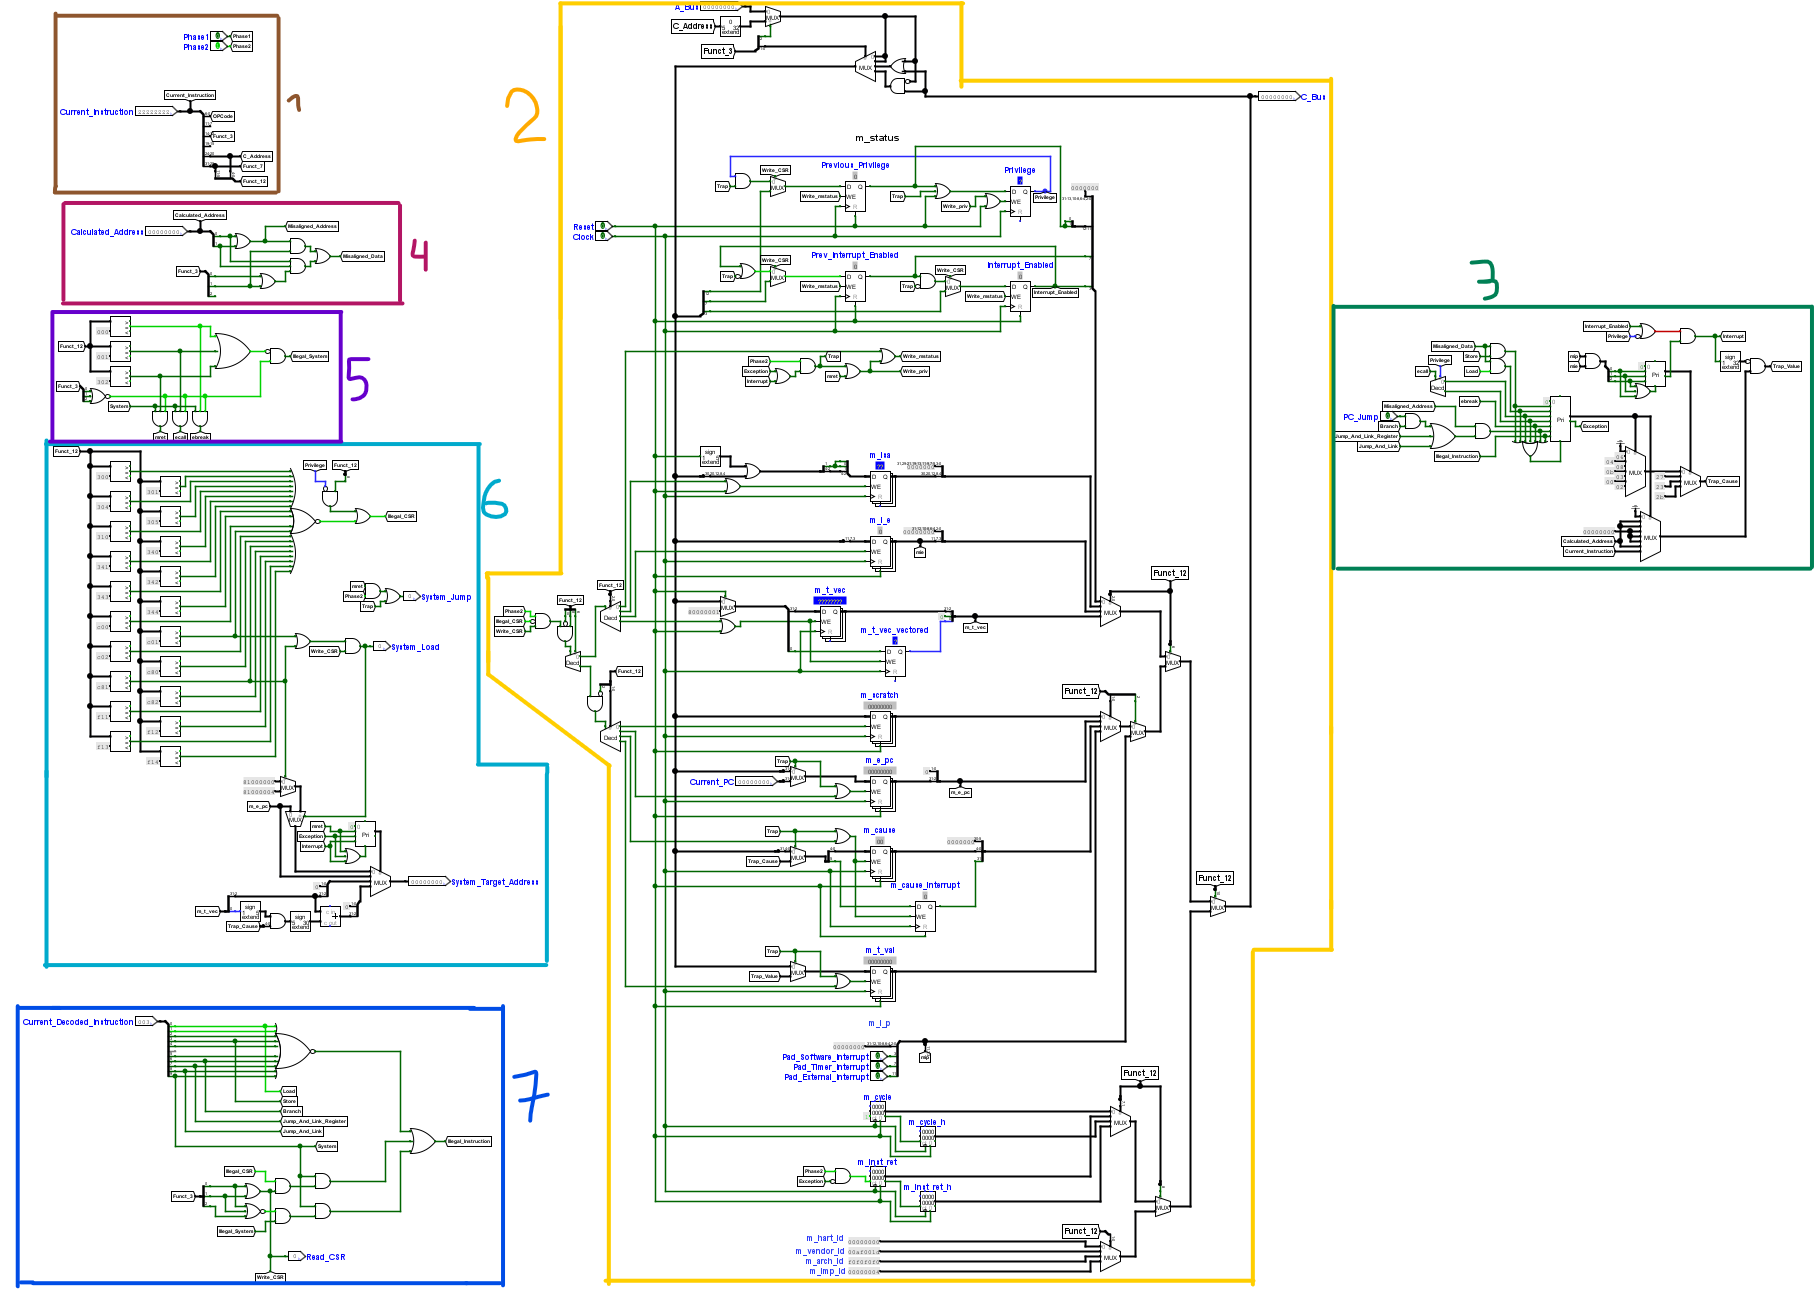
\includegraphics[width=1\linewidth]{ProcessoDesenvolvimento/Arquitetura/CSR_Controller.png}
    \caption{Circuito do Controlador de CSR.}
    \label{fig:Controlador_CSR}
\end{figure}

O circuito do controlador foi projetado seguindo uma ordem lógica semelhante à utilizada no desenvolvimento do código. A primeira etapa envolveu a criação dos registradores e a implementação das funcionalidades de manipulação de dados.

O Circuito 1 processa a entrada da fase e da instrução atual, separando-a em seus respectivos parâmetros. Em paralelo, o Circuito 7 recebe a instrução atual já decodificada, originada diretamente do Controlador de Operações. Neste circuito, alguns sinais são transmitidos para módulos subsequentes, enquanto dois sinais específicos são gerados: o sinal de manipulação de CSR e o sinal de instrução ilegal. Ambos os circuitos estão ilustrados na Figura~\ref{fig:CSR_1_7}.

\begin{figure}[h]
    \centering
    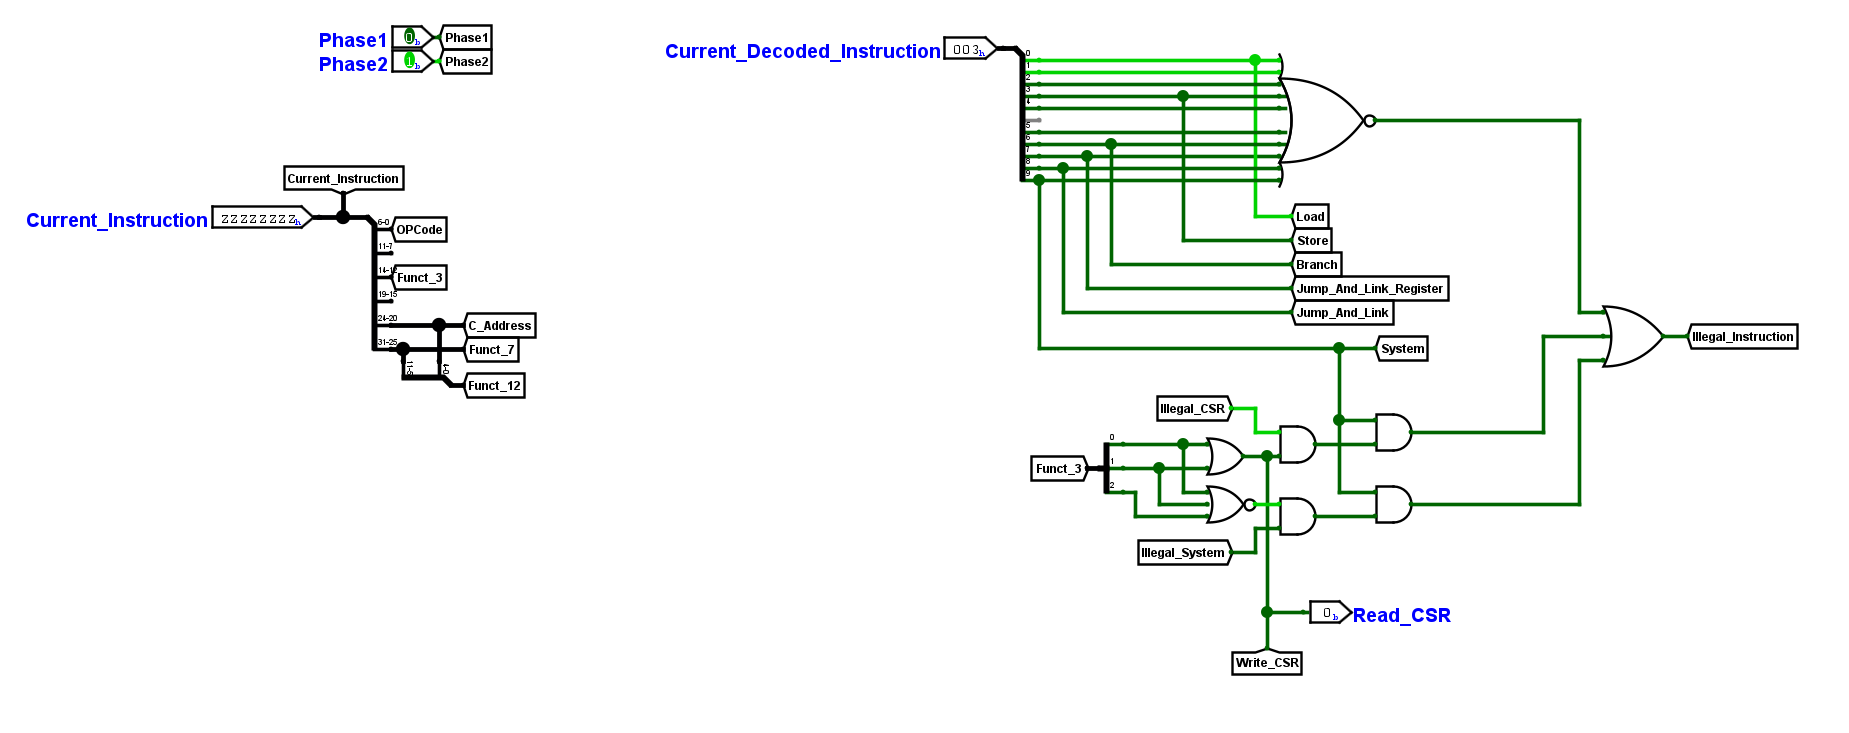
\includegraphics[width=1\linewidth]{ProcessoDesenvolvimento/Arquitetura/CSR_1_7.png}
    \caption{Circuitos de fase, instrução atual e instrução decodificada.}
    \label{fig:CSR_1_7}
\end{figure}

O Circuito 2 é responsável pelo armazenamento e manipulação dos CSRs. Sua lógica de funcionamento simplificada é representada na Figura~\ref{fig:CSR_2}. Cada registrador possui sua escrita ativada por meio de um decodificador conectado a um sinal de controle. Para evitar a criação de um decodificador excessivamente grande, a implementação dividiu esse componente em módulos menores, utilizando apenas alguns dos 12 bits do endereço. Além disso, certos registradores, como aqueles de leitura exclusiva, não são conectados a um decodificador.

As saídas dos registradores são encaminhadas para multiplexadores, que, de maneira análoga à lógica de escrita, utilizam apenas alguns bits para selecionar os registradores apropriados. A saída do último demultiplexador é direcionada tanto para o barramento C quanto para o circuito responsável pelo cálculo do novo valor do CSR.

\begin{figure}[h]
    \centering
    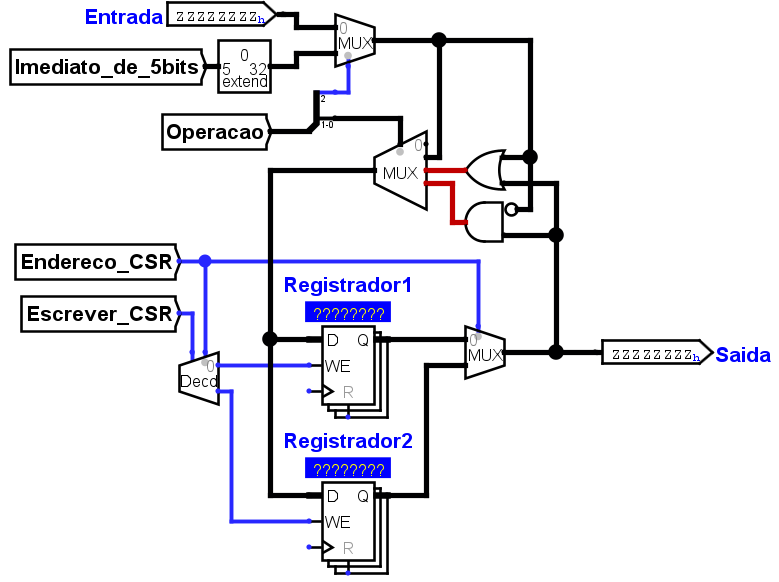
\includegraphics[width=0.75\linewidth]{ProcessoDesenvolvimento/Arquitetura/CSR_2.png}
    \caption{Representação simplificada do circuito de armazenamento e manipulação de CSRs.}
    \label{fig:CSR_2}
\end{figure}

O cálculo do novo valor do CSR segue a lógica estabelecida no Algoritmo \ref{alg:novo_valor_calculado}. O resultado é conectado a todos os registradores, sendo sua entrada proveniente do barramento A ou de um valor imediato de 5 bits (sem sinal), extraído do campo \texttt{Rs2} da instrução.

Os Circuitos 3, 4, 5 (Figura~\ref{fig:CSR_3_4_5}) e parte do Circuito 6 são responsáveis pela lógica assíncrona do tratamento de \textit{traps}. O Circuito 4 detecta endereços desalinhados gerados pelo contador de programas, identificando desalinhamentos para instruções de salto, carregamento e armazenamento. Já o Circuito 5 utiliza os campos \texttt{func\_3} e \texttt{funct\_12} (últimos 12 bits da instrução) para gerar sinais indicativos de instrução de sistema ilegal, além de instruções \texttt{EBREAK}, \texttt{ECALL} e \texttt{MRET}.

\begin{figure}[h]
    \centering
    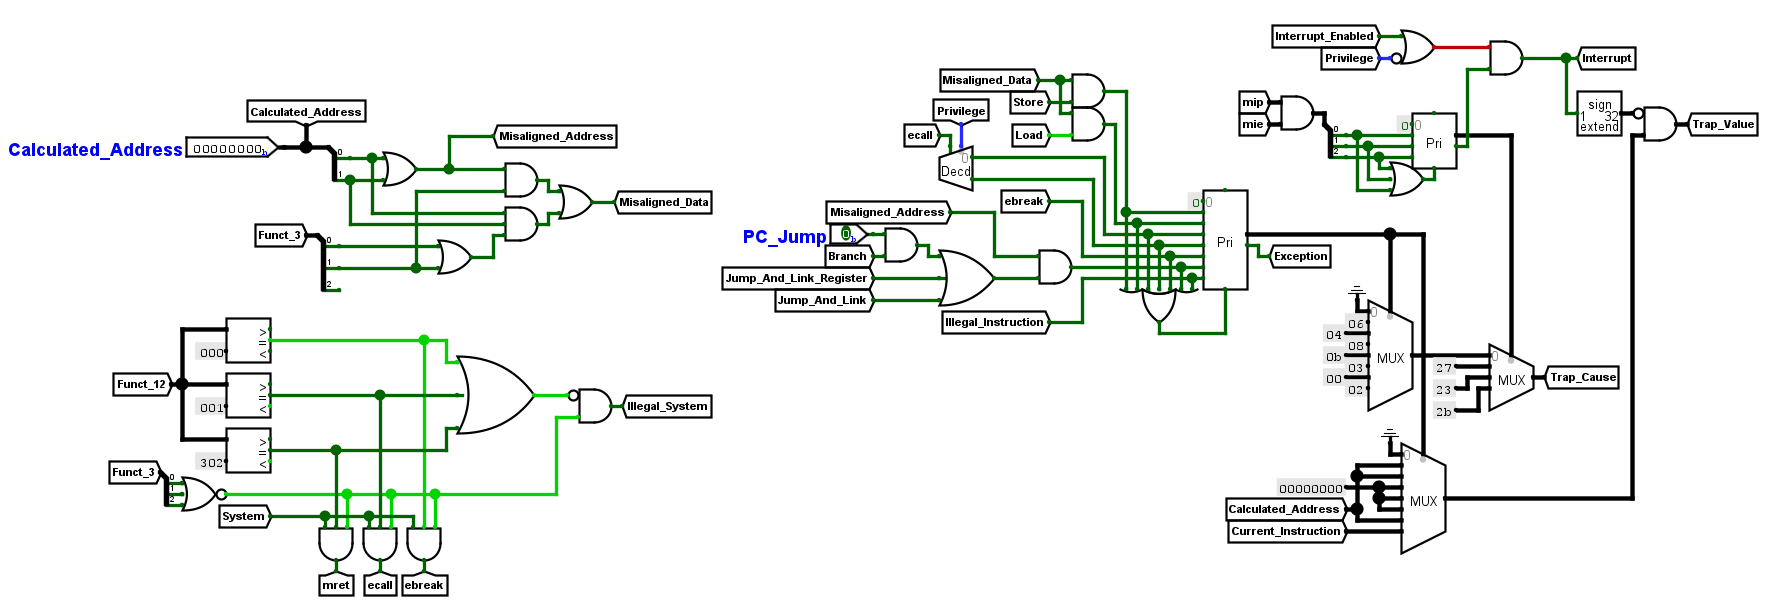
\includegraphics[width=1\linewidth]{ProcessoDesenvolvimento/Arquitetura/CSR_3_4_5_6.png}
    \caption{Circuitos de tratamento de \textit{traps}.}
    \label{fig:CSR_3_4_5}
\end{figure}

Uma parte significativa do Circuito 6 é dedicada à verificação da existência do endereço do CSR da instrução atual, emitindo um sinal de CSR ilegal caso o endereço não seja válido. Esse circuito também identifica tentativas de acesso a CSRs que requerem privilégios elevados, agregando essa informação ao sinal de CSR ilegal.

Por fim, o Circuito 3 é, em sua essência, uma implementação da lógica descrita no Algoritmo \ref{alg:rotina_assincrona}. Ele gera os sinais de exceção e interrupção, bem como os sinais de causa e valor da \textit{trap}. Este circuito incorpora um novo componente do Logisim, o codificador de prioridade, que recebe os vários sinais das possíveis exceções e interrupções e determina automaticamente o endereço do evento com maior prioridade.

A Figura~\ref{fig:CSR_6} apresenta o Circuito 6. A porção superior está relacionada à detecção de CSRs ilegais, enquanto a parte inferior gerencia os sinais de pulo e carregamento de sistema, além de definir o endereço alvo enviado ao contador de programas.

\begin{figure}[h]
    \centering
    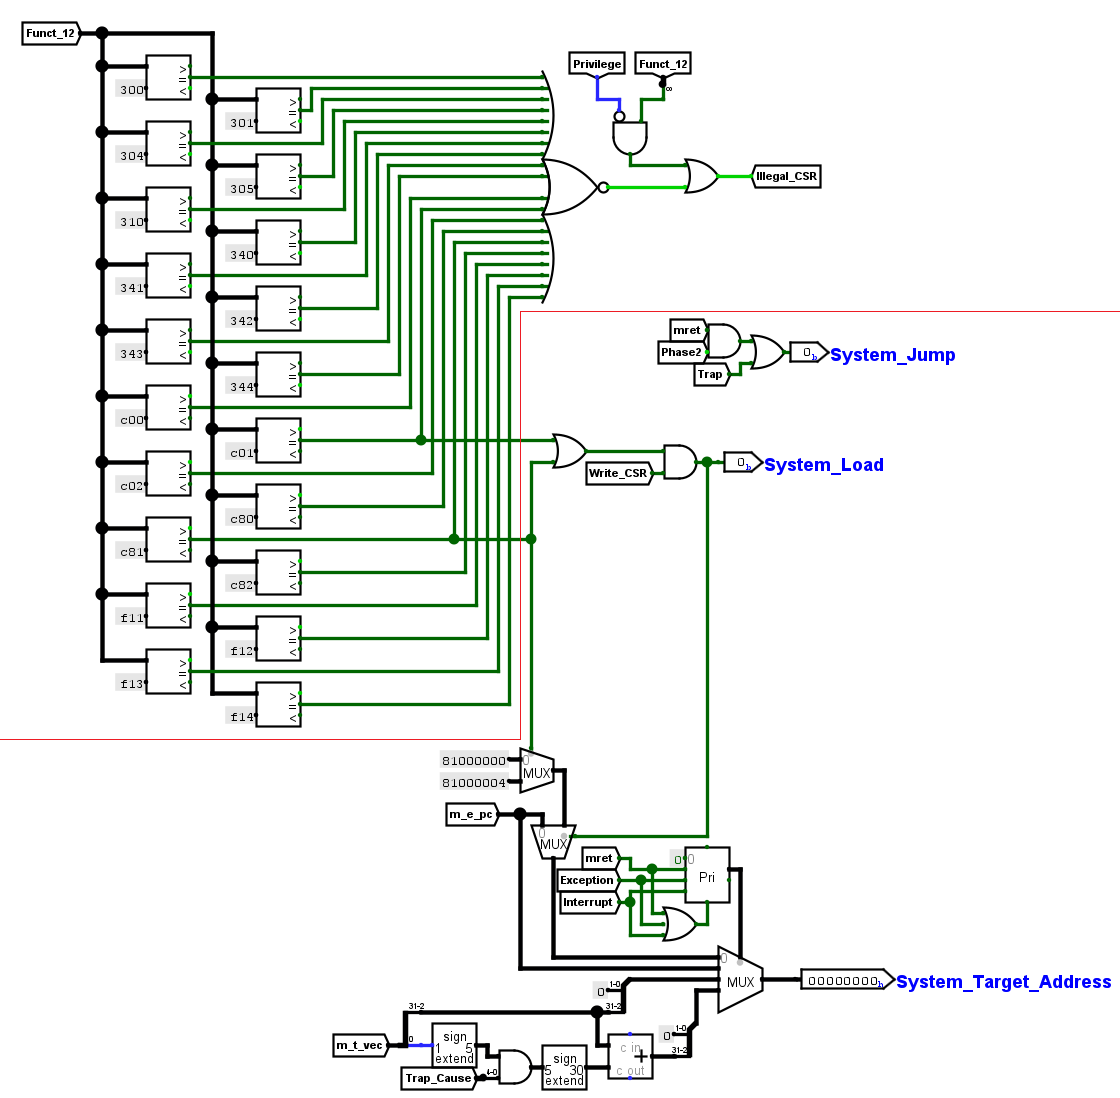
\includegraphics[width=0.5\linewidth]{ProcessoDesenvolvimento/Arquitetura/CSR_6.png}
    \caption{Circuito de verificação de CSRs e controle de sinais de pulo e carregamento.}
    \label{fig:CSR_6}
\end{figure}

A Figura~\ref{fig:CSR_Controller_Visual} apresenta o encapsulamento visual do controlador. Nela, é possível observar os valores de todos os CSRs escrevíveis. Bits não utilizados (sempre 0) não são exibidos. Pequenas legendas foram adicionadas aos registradores MISA e MIE para indicar o significado dos valores. O bit de privilégio foi posicionado ao lado do registrador \texttt{MSTATUS}, pois, apesar de não estar incluído no CSR, trata-se de uma informação relevante.

\begin{figure}[h]
    \centering
    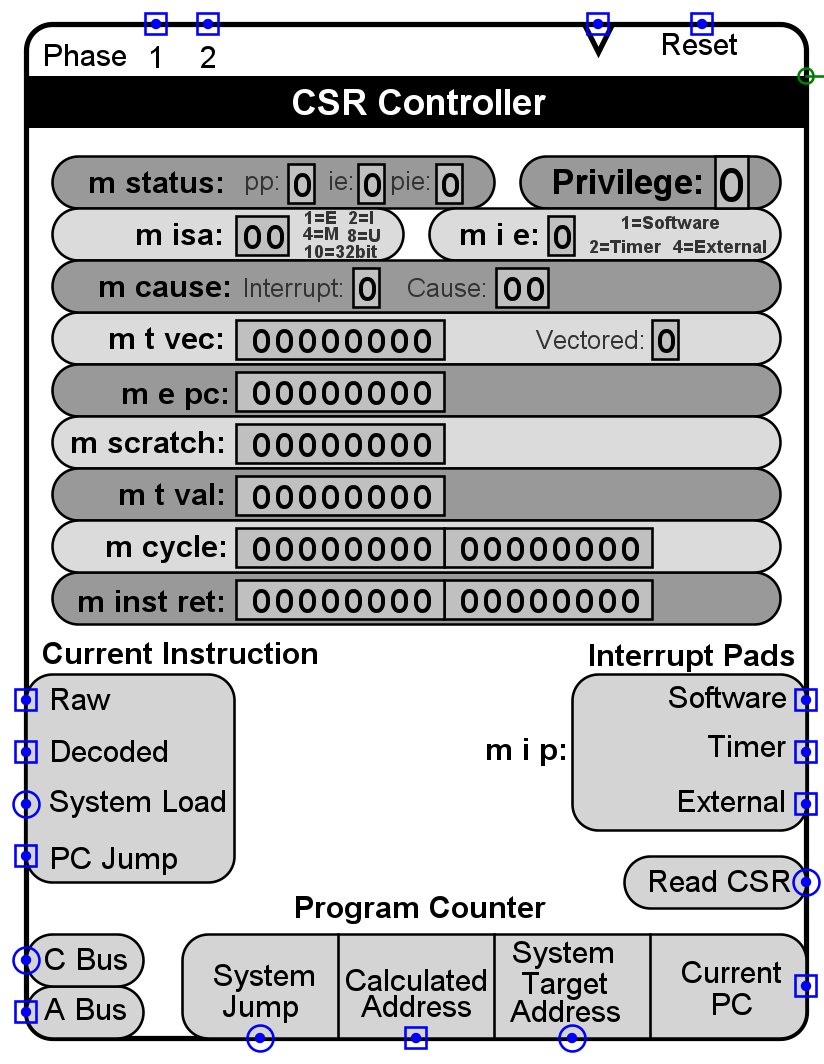
\includegraphics[width=0.5\linewidth]{ProcessoDesenvolvimento/Arquitetura/CSR_Controler_Component.png}
    \caption{Encapsulamento do Controlador de CSR}
    \label{fig:CSR_Controller_Visual}
\end{figure}

A interface com o Controlador de Operações foi mantida à esquerda, enquanto a interface com o Contador de Programas permaneceu na parte inferior do componente. Os sinais de interrupção foram posicionados à direita, permitindo uma melhor organização do circuito geral, conforme ilustrado na Figura~\ref{fig:CSR_Integrated}. Durante o desenvolvimento do novo componente, foram utilizados os mesmos programas de teste empregados na simulação SV.

\begin{figure}[h]
    \centering
    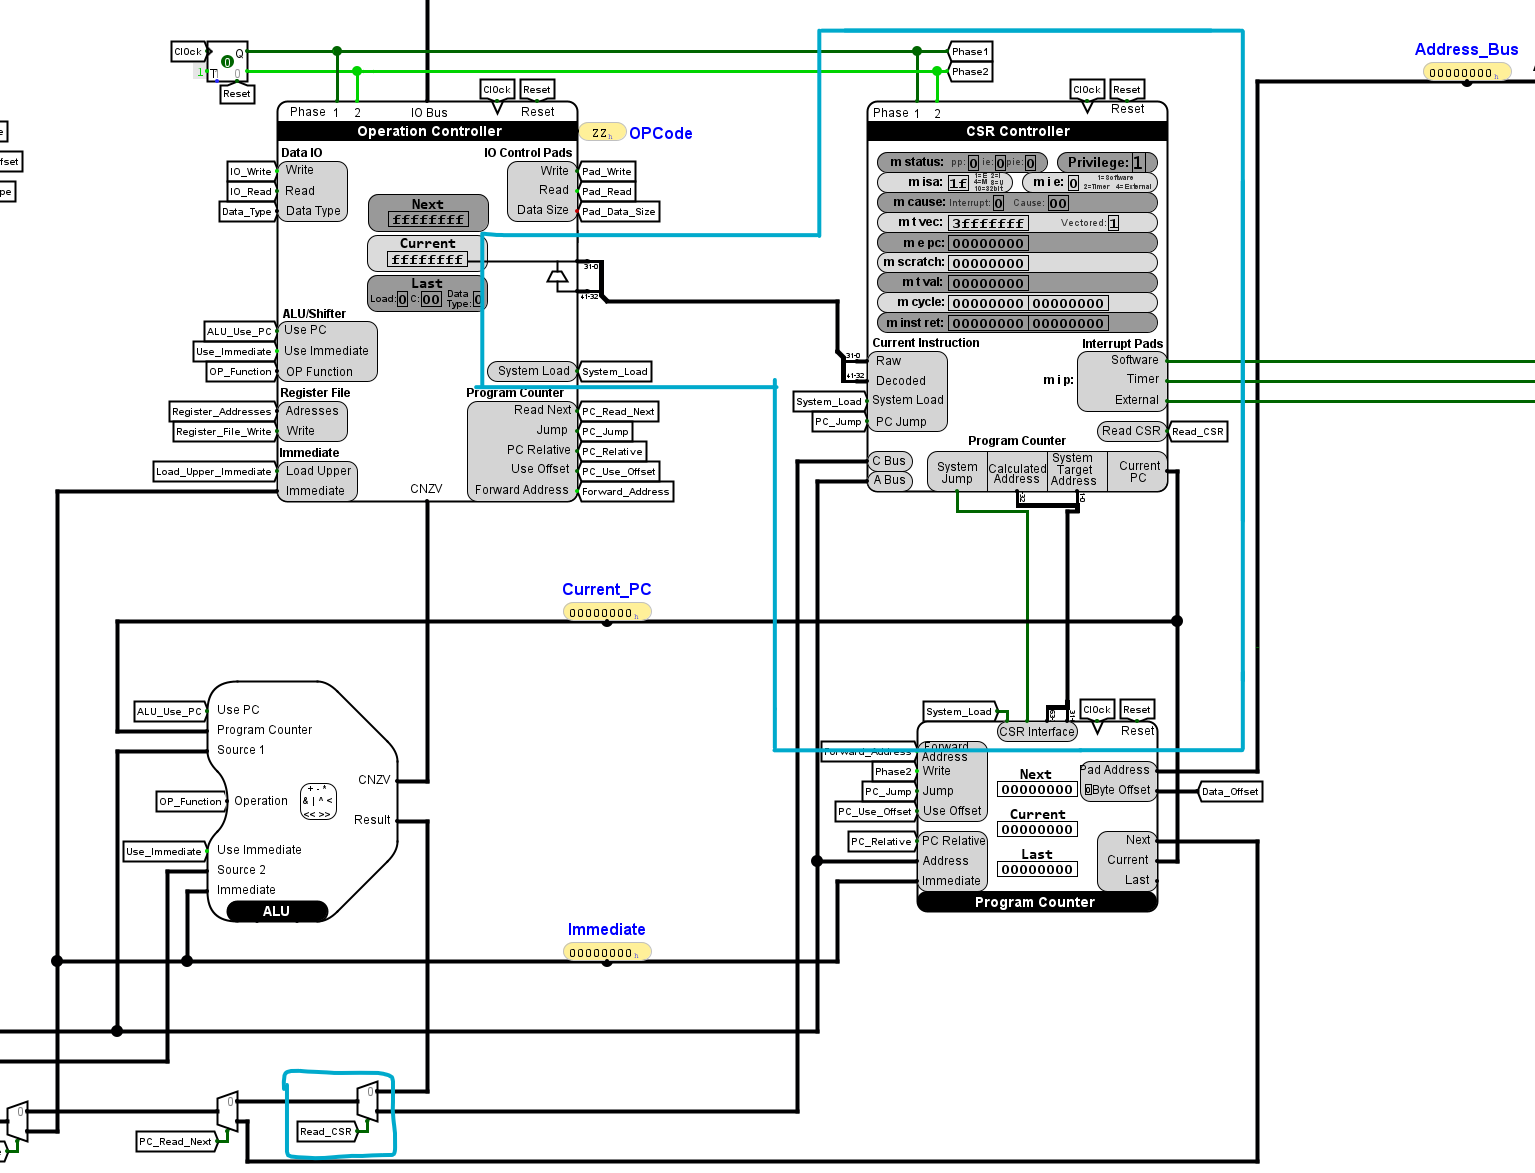
\includegraphics[width=0.75\linewidth]{ProcessoDesenvolvimento/Arquitetura/IntegraçãoControladorCSR.png}
    \caption{Integração do Controlador de CSR na arquitetura}
    \label{fig:CSR_Integrated}
\end{figure}

Um dos CSRs mencionados anteriormente, o TIME (e, consequentemente, o TIMEH), é mapeado na memória do processador, e não no próprio processador. Isso significa que, para acessá-lo, é necessário executar uma instrução de carregamento ou salvamento. Como mostrado anteriormente, a leitura do CSR pode ser realizada através de uma instrução de manipulação de CSR, utilizando o mecanismo criado de carregamento de sistema.

Esse CSR desempenha um papel crucial no mecanismo de interrupção por tempo do processador. Ele opera por meio de dois registradores de 64 bits: um que armazena o tempo atual (\texttt{m\_time}) e outro que define o tempo da próxima interrupção (\texttt{m\_cmp\_time}) \cite[p.5]{risc-v_risc-v_2022}. Quando \texttt{m\_time} ultrapassa \texttt{m\_cmp\_time}, um sinal de interrupção é enviado ao processador por meio de um fio de controle.

Na implementação pela simulação SV, o componente responsável pelo armazenamento e controle desses registradores recebeu um sinal de clock secundário, encarregado da incrementação de \texttt{m\_time}. Esse clock pode ser configurado com uma frequência maior ou menor que o restante da simulação. Frequências mais altas, em até 10 vezes o clock do processador, não impactam significativamente a performance. No entanto, frequências excessivamente elevadas causaram degradação no desempenho.

\begin{figure}[h]
    \centering
    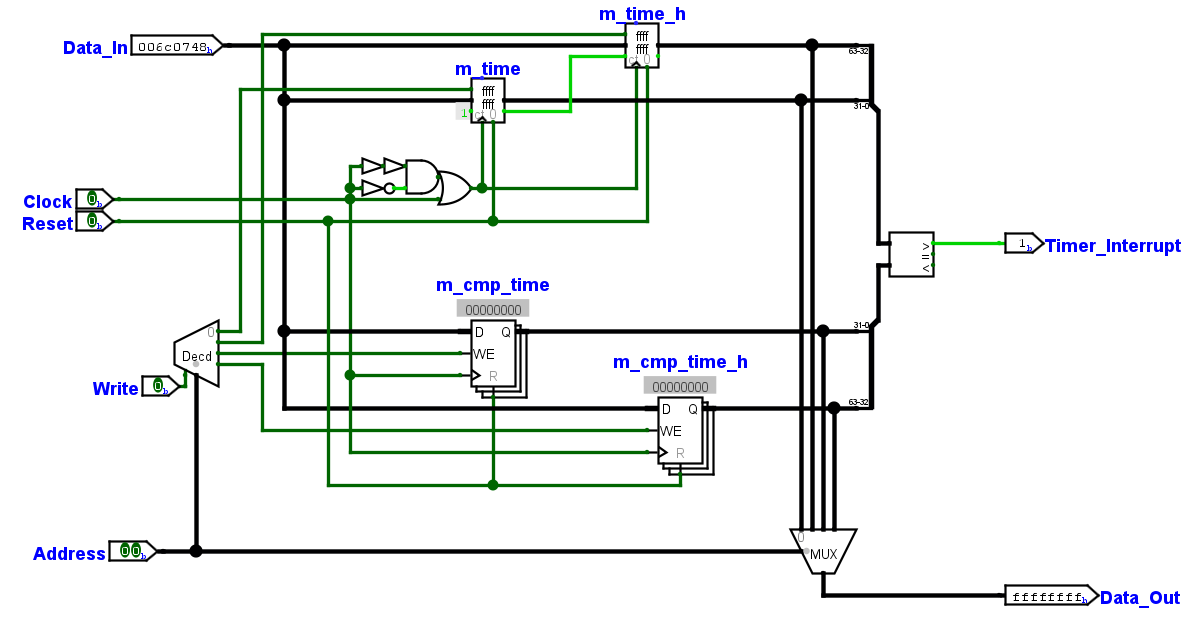
\includegraphics[width=0.75\linewidth]{ProcessoDesenvolvimento/Arquitetura/RealTimeDevice.png}
    \caption{Circuito do Dispositivo de Tempo Real}
    \label{fig:RTD_Circuit}
\end{figure}

Já no Logisim (Figura~\ref{fig:RTD_Circuit}), não é possível gerar um clock com frequência diferente sem a criação de componentes customizados. A redução da frequência do processador também não foi viável, pois a simulação do Logisim já operava em uma frequência bastante baixa, entre 30 e 60 Hertz. Para simular frequências mais altas, foi utilizado um gerador de pulso ativado na borda de descida do \textit{clock}. Esse mecanismo, combinado com o sinal de \textit{clock} normal, efetivamente dobra os sinais responsáveis pela incrementação de \texttt{m\_time}.

O gerador de pulso consiste em dois \textit{buffers}, uma porta \texttt{NÃO} e uma porta \texttt{E}. Quando o sinal de clock é recebido, uma das entradas da porta \texttt{E} é atualizada primeiro, ativando temporariamente a porta antes que a outra entrada seja ajustada.

Os registradores são mapeados contiguamente na memória a partir do endereço \texttt{0x81000000} e são divididos em porções de 32 bits, permitindo operações de leitura e escrita. A Figura~\ref{fig:RTD_Component} ilustra o componente desenvolvido e suas interfaces. A entrada de endereços recebe os bits 2 e 3 do endereço de memória, garantindo o mapeamento correto de cada registrador em blocos de 4 bytes.

\begin{figure}[h]
    \centering
    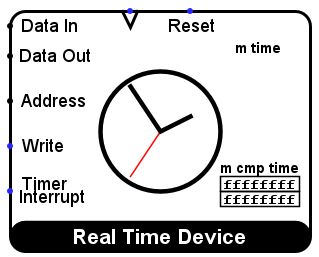
\includegraphics[width=0.25\linewidth]{ProcessoDesenvolvimento/Arquitetura/RealTimeDeviceComponent.png}
    \caption{Encapsulamento do Dispositivo de Tempo Real}
    \label{fig:RTD_Component}
\end{figure}

O registrador responsável pela interrupção por software \cite[p.8]{risc-v_risc-v_2022} foi implementado de maneira simplificada, utilizando apenas um \textit{flip-flop}. Esse registrador pode ser modificado por meio de instruções de armazenamento no endereço \texttt{0x81000010}, logo após o último endereço do Dispositivo de Tempo Real. A Figura~\ref{fig:SoftwareInterruptReg} apresenta a implementação do registrador.

\begin{figure}[h]
    \centering
    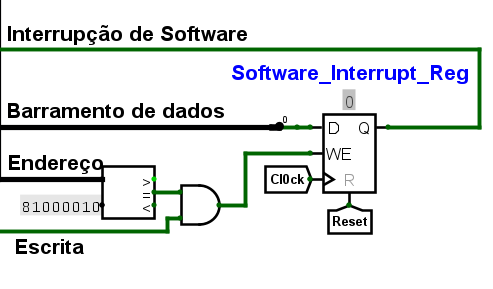
\includegraphics[width=0.5\linewidth]{ProcessoDesenvolvimento/Arquitetura/SoftwareInterruptRegister.png}
    \caption{Registrador de Interrupção de Software}
    \label{fig:SoftwareInterruptReg}
\end{figure}

\subsubsection{Sexta Fase: Pipeline}

Perto do fim do desenvolvimento do controlador de CSR, foi criado um programa para a arquitetura, com o objetivo de processar as possíveis exceções e interrupções que podem ocorrer durante a execução de outros programas. Esse programa é o \textit{Trap~Handler}, o qual é executado assim que uma exceção ocorre ou no ciclo seguinte à ocorrência de um sinal de interrupção. Na implementação atual, ele deve estar armazenado no endereço indicado pelo CSR \texttt{mtvec}, inicializado como \texttt{0x80000000}.

O \textit{Trap~Handler} foi inicialmente implementado de forma simples, lidando apenas com exceções e imprimindo-as no terminal. O objetivo era tanto apresentar um exemplo básico de como os erros são processados no sistema quanto viabilizar uma forma prática de testar se todas as exceções estavam sendo tratadas corretamente.

Durante o desenvolvimento, verificou-se que, apesar de o \textit{Trap~Handler} ser chamado e executado corretamente, o processador continuava a executar as instruções até o fim, comportamento incorreto que poderia causar outros erros. Esse problema fazia com que instruções de carregamento, salvamento e desvio fossem executadas completamente, mesmo quando geravam exceções, resultando em modificações indesejadas nos registradores e na memória.

Para corrigir esse problema, um sinal de exceção deveria ser transmitido do controlador de CSR para o controlador de operações, que então deveria desativar os sinais correspondentes às instruções afetadas. Durante esse processo, decidiu-se implementar uma correção que alteraria a forma como esse recurso seria integrado. Essa correção diz respeito a um equívoco cometido na implementação da \textit{Pipeline} do processador, presente desde sua primeira versão.

O erro consistia em posicionar o registrador da instrução atual antes da etapa de decodificação. Embora esse equívoco já tivesse sido identificado anteriormente, não havia sido corrigido por não causar problemas nas simulações. No entanto, em um processador real, isso poderia limitar o tempo disponível para decodificar a instrução antes de sua execução, comprometendo a frequência máxima de operação e eliminando qualquer ganho proporcionado pela pipeline.

Inicialmente, as alterações foram planejadas apenas no controlador de operações, já que o controlador de CSR possui grande complexidade e não é essencial para o funcionamento básico do processador. O planejamento buscou utilizar o menor número possível de registradores, alocados o mais próximo possível dos sinais de controle, imediatamente antes das portas lógicas conectadas aos sinais de fase.

O registrador da instrução atual foi mantido, tanto por conter informações que não exigem decodificação lógica quanto por ser utilizado pelo controlador de CSR. Além disso, foram adicionados registradores associados diretamente a instruções específicas, como \texttt{load}, \texttt{store}, \texttt{branch}, \texttt{LUI} (Load Upper Immediate), \texttt{AUIPC} (Add Upper Immediate to PC), bem como registradores compartilhados entre múltiplas instruções, como para desvios não condicionais (\texttt{JAL} e \texttt{JALR}), instruções relativas ao endereço atual (\texttt{Branch} e \texttt{JAL}), dois registradores para instruções da ULA, e um registrador para controle de escrita no arquivo de registradores e um registrador para o valor imediato.

O controlador de programa também inclui três registradores introduzidos em etapas anteriores, os quais substituem o registrador da última instrução. Esses registradores são específicos para instruções de carregamento, únicas a possuírem um terceiro ciclo na pipeline. São eles: o registrador de \texttt{load} anterior, o endereço do registrador c alvo e o registrador de tipo de dado (tamanho e sinal).

Alguns sinais de controle não utilizaram registradores ou foram alocados ainda com uma ou duas portas lógicas após os registradores. Isso se deve ao fato de que esses sinais são gerados durante a fase de execução ou precisariam de mais um registrador que aumentaria a complexidade do circuito sem melhorias significativas na velocidade de decodificação. A Figura~\ref{fig:Controlador_Pipeline_Fix} ilustra o novo controlador de operações, com as devidas correções à pipeline.

\begin{figure}[h]
    \centering
    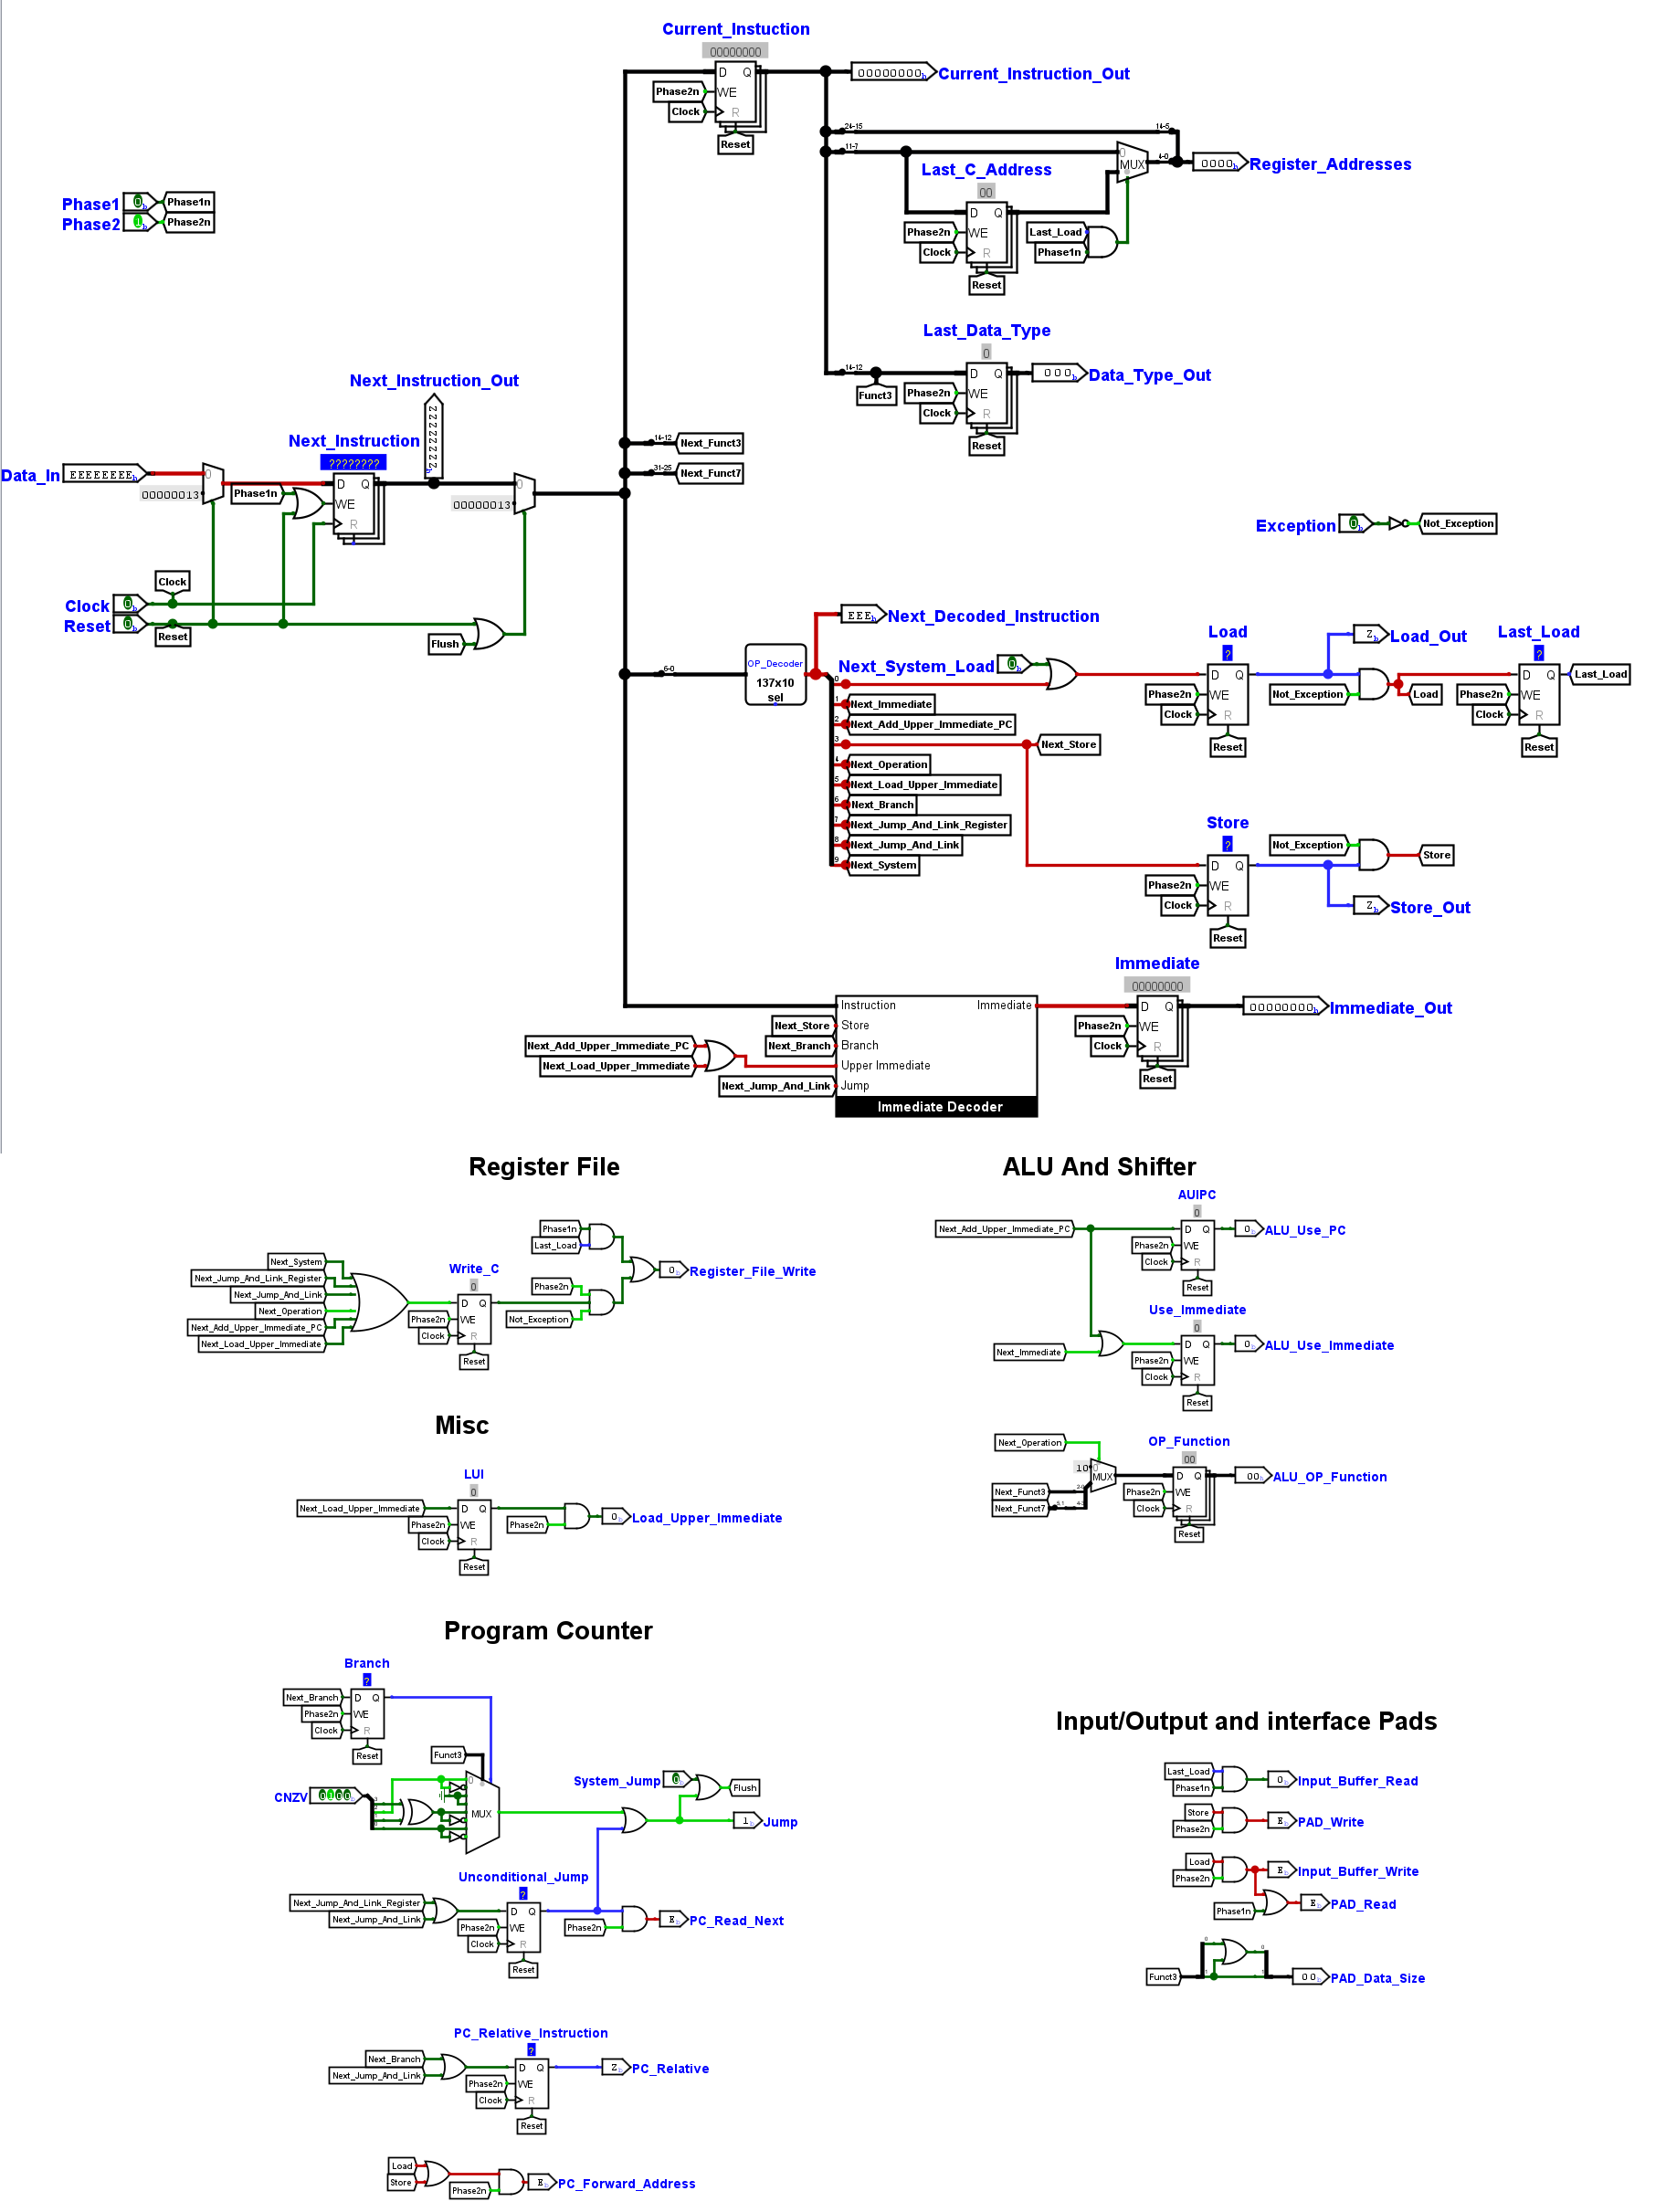
\includegraphics[width=0.95\textwidth]{ProcessoDesenvolvimento/Arquitetura/Controlador_Pipeline_Fix.png}
    \caption{Controlador de Operações com \textit{Pipeline} Corrigida.}
    \label{fig:Controlador_Pipeline_Fix}
\end{figure}

Além dos registradores adicionados, é possível ver a implementação do sinal de exceção, que assim que ativado, impede que os sinais de carregamento, salvamento e escrita no Arquivo de Registradores continuem ativados. Isso evita os efeitos colaterais provenientes de instruções que causam exceções.

Com o controlador de operações corrigido, o próximo passo foi a revisão do controlador de CSR. Devido à sua complexidade, as alterações iniciais foram realizadas por meio do código em SV. O foco dessas modificações foi o mesmo aplicado ao controlador de instruções: mover o máximo possível da etapa de decodificação para o primeiro ciclo da pipeline. Para isso, realizou-se primeiramente uma análise do circuito, visando identificar quais sinais são gerados na fase de decodificação e quais são processados durante a execução da instrução.

Os sinais marcados para decodificação no controlador de CSR são aqueles relacionados às instruções seguintes, incluindo se a próxima instrução é uma instrução de sistema (\texttt{mret}, \texttt{ecall}, \texttt{ebreak} e \texttt{csrrw}) ou se é uma instrução ilegal. As demais informações necessárias são fornecidas pelo controlador de operações e abrangem o valor da palavra da próxima instrução, o valor da instrução atual, a próxima instrução já decodificada, e se a instrução atual corresponde a um \texttt{load}, \texttt{store} ou se está executando um desvio.

A Figura~\ref{fig:Controlador_CSR_Pipeline_Fix} apresenta os circuitos que receberam registradores adicionais no controlador de CSR. Nota-se que, em comparação com versões anteriores, quase todos os sinais de entrada foram modificados para refletirem valores referentes à próxima instrução.

A única exceção a essa regra é o teste de privilégio ao acessar os CSRs, pois a única maneira de o nível de privilégio ser alterado é mediante uma \textit{trap} ou através da instrução \texttt{mret}. Após um desses eventos ocorrer, um desvio é executado, e como desvios são sempre seguidos por um ciclo de instrução vazio (\texttt{nop}), torna-se impossível que o privilégio seja modificado entre duas instruções consecutivas.

\begin{figure}[h]
    \centering
    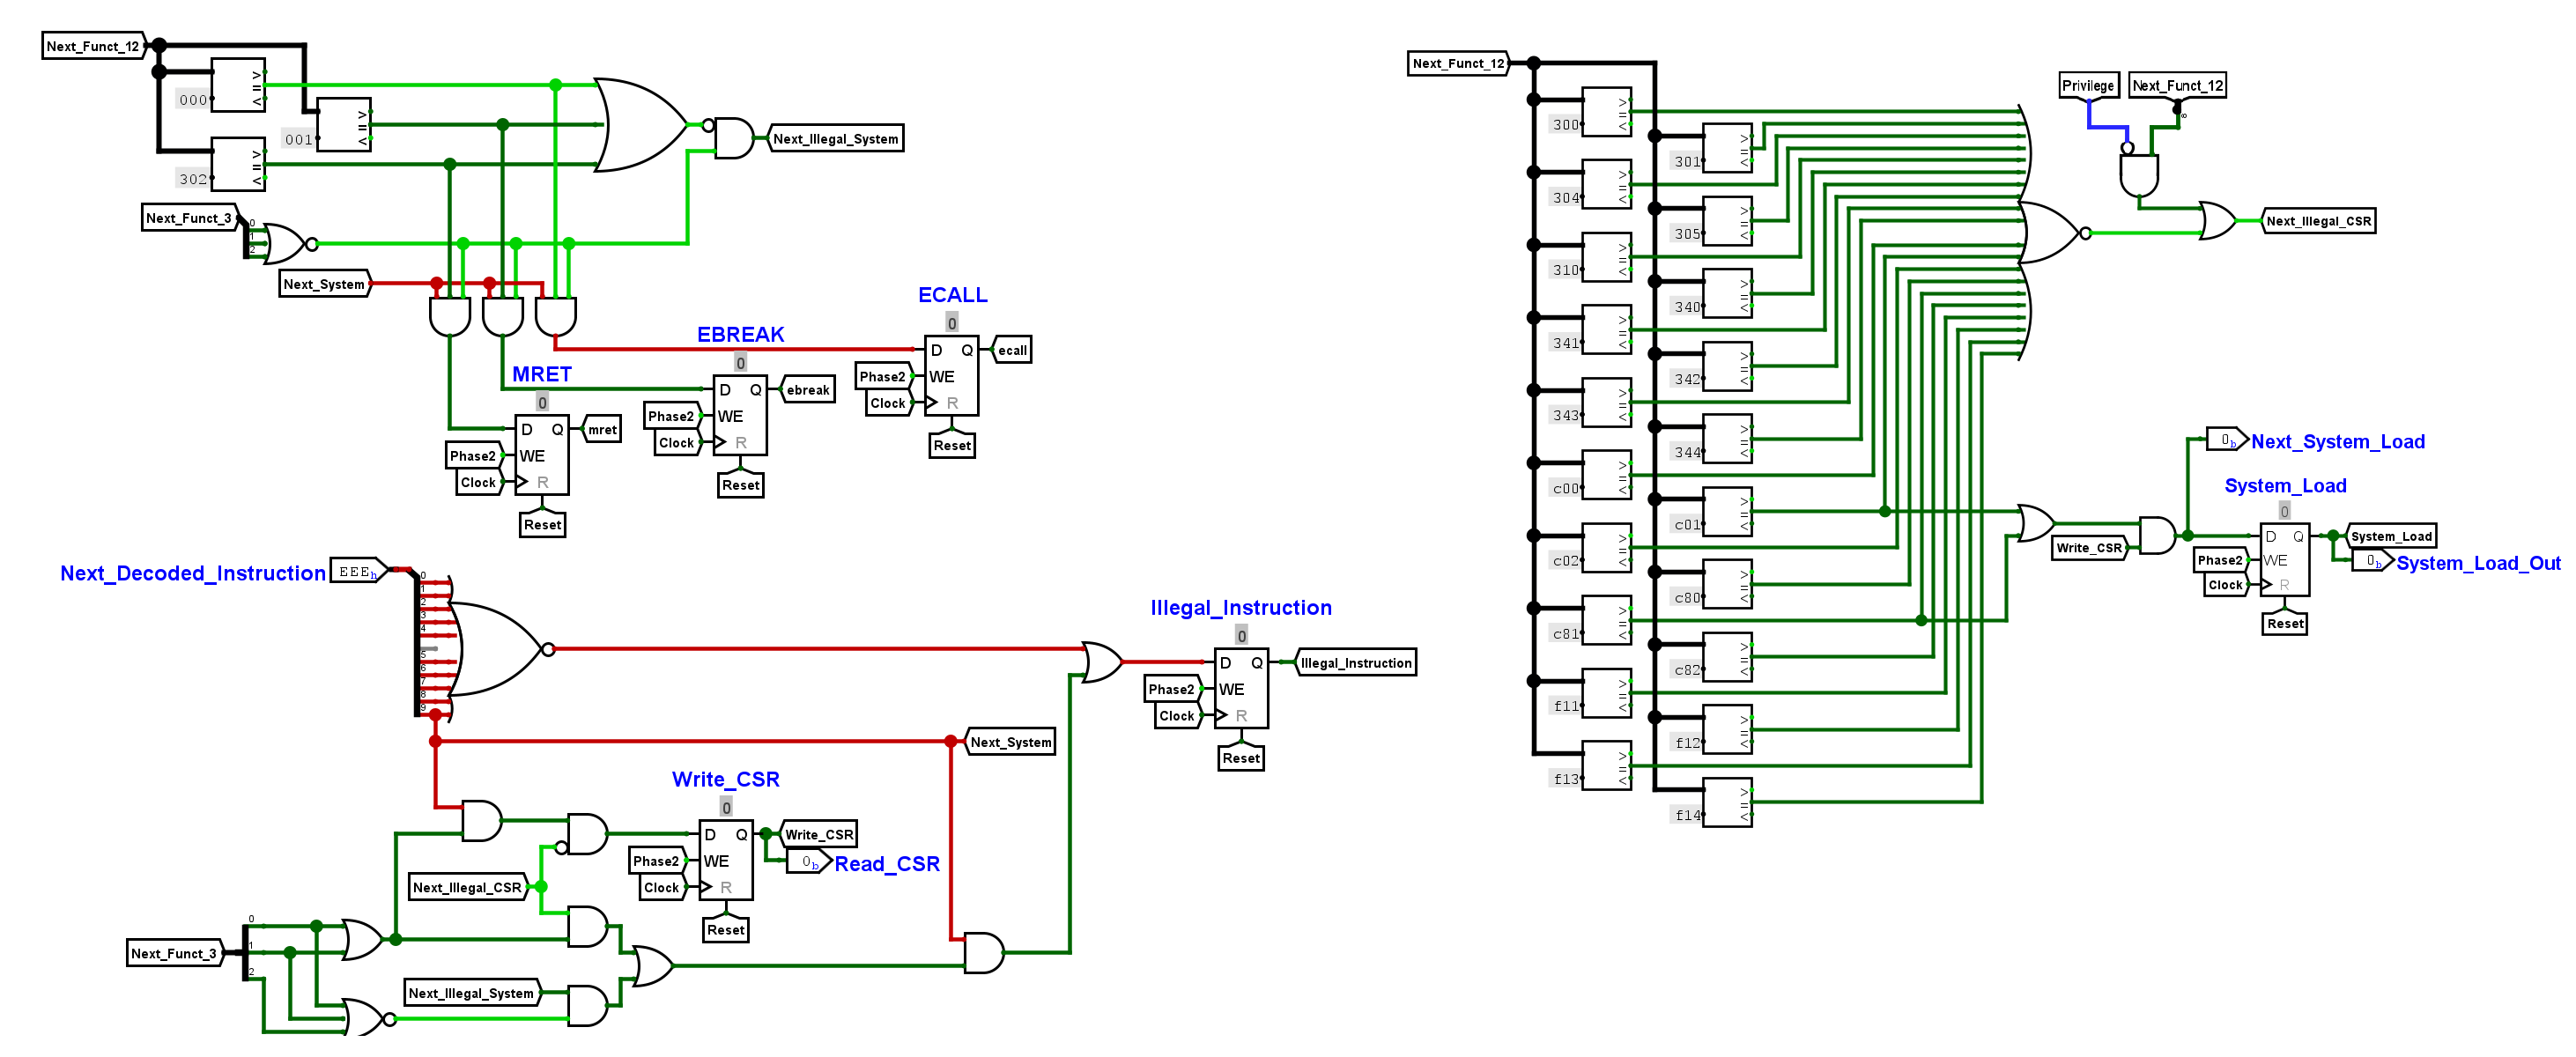
\includegraphics[width=0.95\textwidth]{ProcessoDesenvolvimento/Arquitetura/CSR_Controller_Pipeline_Fix1.png}
    \caption{Controlador de Operações com \textit{Pipeline} Corrigida.}
    \label{fig:Controlador_CSR_Pipeline_Fix}
\end{figure}

Durante as correções executadas, outro componente que foi modificado foi o Contador de Programa. Foi observado que os sinais de pulo eram sempre ativados durante a segunda fase do pipeline. No entanto, não era necessário combinar o sinal de fase nos controladores, pois o próprio Contador de Programa já recebia esse sinal para atualizar seu registrador interno por meio do sinal \texttt{write}.

Dessa forma, o sinal \texttt{write} foi combinado diretamente com os sinais de desvio dentro do próprio contador, o que resultou na simplificação de algumas partes do circuito. As modificações realizadas no Contador de Programa estão detalhadas no Código~\ref{lst:pc_counter_pipeline_fix}.

\begin{lstlisting}[language=Verilog, caption={Alterações realizadas no Contador de Programa}, label={lst:pc_counter_pipeline_fix}]
//antes:
        if(reset) [...]
        else if(system_jump) next_reg <= system_address_target[31:2];
        else if(jump) next_reg <= calculated_address[31:2];
        else if(write) next_reg <= next_reg + 1;

        if(write)
            last_reg <= current_reg;
            current_reg <= next_reg;
        end
//depois:
        if(reset) [...]
        else if(write) begin
            if(system_jump) next_reg <= system_address_target[31:2];
            else if(jump) next_reg <= calculated_address[31:2];
            else next_reg <= next_reg + 1;

            current_reg <= next_reg;
        end
\end{lstlisting}

Por fim, outra modificação realizada foi a remoção do registrador responsável por armazenar a última instrução no Contador de Programa. Após alterações estruturais em passos anteriores, esse registrador deixou de ter relevância na arquitetura e, portanto, pôde ser eliminado sem impactos funcionais.

Durante o processo de desenvolvimento dessa fase, melhorias foram realizadas no código SV para impressão de mensagens mais informativas. Alterações inclusas foram a adição de uma coluna para exibir valores decimais com sinal ao lado de cada registrador e a adição de uma coluna com valores ASCII correspondentes a cada byte da memória RAM, que podem ser vistos na Figura~\ref{fig:SV_Print_Upgrade}.

\begin{figure}[h]
    \centering
    \includegraphics[width=0.75\textwidth]{ProcessoDesenvolvimento/Arquitetura/SV_Print_Upgrade.png}
    \caption{Saída do programa de teste com melhorias na impressão.}
    \label{fig:SV_Print_Upgrade}
\end{figure}

Também foi adicionado uma opção para desativar a geração do do controlador de CSR no processador no código SV, permitindo uma execução mais simplificada de programas que não utilizam interrupções ou exceções.

\subsection{Processo de Desenvolvimento - Assembler}\label{process_assembler}

O desenvolvimento do \textit{assembler} foi realizado paralelamente ao desenvolvimento da arquitetura. Inicialmente, o objetivo era obter uma forma de criar programas para que pudessem ser executados nos simuladores. Esse objetivo se tornou menos relevante quando o padrão RISC-V foi adotado, pela existência de outros \textit{assemblers} mais completos que poderiam ser utilizados.

Logo, o objetivo foi obter um \textit{assembler} mais simples, que pudesse exibir como que as instruções são traduzidas para o código de máquina, e que fornecesse informações importantes para o \textit{debugging} de programas, como o endereço de cada instrução.

Além de melhorias no código de tradução de instruções, foram realizadas melhorias no código de pré processamento de código, com aperfeiçoamentos na remoção de espaços em branco e comentários e a adição de suporte para \textit{macros} e \textit{defines}, que facilitam a criação de código repetitivo e definições que facilitam a leitura do código.

\subsubsection{Adaptação para RISC-V}

A primeira versão do \textit{assembler} apresentava limitações significativas, pois utilizava um processo de decodificação fixo para todas as instruções, o que dificultava a adição ou modificação de formatos diferentes. No caso do RISC~I, isso não representava um problema, uma vez que havia apenas dois formatos de instrução: \texttt{OPCode~<rd|cond>~<rs1>~<rs2|Imediato13>} e \texttt{OPCode~<rd>~<imediato-19>}. Contudo, no RISC-V existem diversos outros formatos, além de pseudoinstruções definidas especificamente para \textit{assemblers}\cite{risc-v_risc-v_2025}.

Para solucionar essa limitação, foi realizada uma reescrita do \textit{assembler}. Em vez de adotar uma tradução fixa, a nova versão passou a utilizar \textit{dicionários} de funções de tradução. Assim, para adicionar novas instruções, basta incluí-las no dicionário, usando o nome como chave e associando a ele uma função que recebe uma lista de parâmetros como entrada e retorna o código de máquina correspondente como saída.

Essa abordagem não apenas ampliou a flexibilidade na criação de novas instruções, mas também possibilitou a visualização direta de todas as instruções disponíveis no \textit{assembler}, por meio de uma lista no próprio código.

Nas versões mais recentes, esse comportamento foi aprimorado para permitir que uma pseudoinstrução pudesse ser traduzida em múltiplas instruções. Para isso, adotou-se um dicionário de funções geradoras, responsáveis por criar as funções de tradução necessárias durante o processo de montagem.

Por exemplo, ao acessar uma determinada instrução no dicionário, obtém-se uma função \texttt{geradorDeTradutor(string[] parâmetros)}, que por sua vez retorna uma lista de funções. Cada função dessa lista, quando executada, gera o valor numérico de uma instrução necessária para a implementação completa da pseudoinstrução.

Embora a maioria das instruções seja traduzida para apenas uma instrução de máquina, existem pseudoinstruções que podem gerar mais de uma, como \texttt{li}, \texttt{la} e \texttt{call}.

As funções de tradução foram implementadas a partir de funções genéricas, responsáveis por converter os formatos comuns de instrução especificados por \citeonline{risc-v_risc-v_2024}, conforme ilustrado na Figura~\ref{fig:InstructionFormatRISCV}.

\begin{figure}[h]
    \centering
    \includegraphics[width=0.95\textwidth]{ProcessoDesenvolvimento/Assembler/InstructionFormat.png}
    \caption{Formatos de instrução base do RISC-V~\cite{risc-v_risc-v_2024}.}
    \label{fig:InstructionFormatRISCV}
\end{figure}

Para utilizar essas funções genéricas, é necessário fornecer determinados parâmetros. Todos os parâmetros relacionados ao tipo de instrução foram definidos como enumeráveis, facilitando a tradução e garantindo melhor legibilidade. Entre eles estão: instruções base, nomes de registradores, operações matemáticas, tipos de comparação para instruções de desvio, tamanhos de dados, funções de sistema e nomes de CSR.

Já os parâmetros correspondentes a valores numéricos são fornecidos como texto, de forma que possam ser processados por um método específico capaz de diferenciar automaticamente valores hexadecimais e decimais.

\subsubsection{Variáveis}

Foi adicionado suporte à declaração de variáveis com tipos numéricos de 8, 16 e 32 bits, além de \textit{strings}. Essas variáveis são decodificadas por meio de um dicionário com estrutura semelhante ao utilizado para instruções, permitindo que cada variável possua um nome opcional e/ou uma sequência de valores contíguos na memória.

A Tabela~\ref{tab:DeclaracoesVariaveis} apresenta exemplos de declarações válidas:
\begin{table}[h]
    \centering
    \caption{Exemplos de declarações de variáveis e seus valores em compilados}
    \label{tab:DeclaracoesVariaveisHexCorrigida}
    \begin{tabular}{lll}
        \toprule
        \textbf{Tipo} & \textbf{Declaração} & \textbf{Valor Compilado} \\
        \midrule
        \texttt{.string} & \texttt{.string teste "uma string"} &
        \begin{tabular}[c]{@{}l@{}}
        \texttt{756b6120}-\texttt{73747269}-\texttt{6e670000}
        \end{tabular} \\
        & \texttt{.string "a string"} &
        \begin{tabular}[c]{@{}l@{}}
        \texttt{61207374}-\texttt{72696e67}-\texttt{00000000}
        \end{tabular} \\
        & \texttt{.string "1"} & \texttt{00000031} \\
        \texttt{.word} & \texttt{.word umInteiro 0x03bb00ff} & \texttt{03bb00ff} \\
        & \texttt{.word umVetor 1 2 3} &
        \begin{tabular}[c]{@{}l@{}}
        \texttt{00000001}-\texttt{00000002}-\texttt{00000003}
        \end{tabular} \\
        \texttt{.half} & \texttt{.half umHalf 0xffff} & \texttt{0000ffff} \\
        & \texttt{.half umVetorHalf 0xffff 0xeeee 0xCCCC} &
        \begin{tabular}[c]{@{}l@{}}
        \texttt{eeeeffff}-\texttt{0000CCCC}
        \end{tabular} \\
        & \texttt{.half 0xffff} & \texttt{0000ffff} \\
        \texttt{.byte} & \texttt{.byte umByte 128} & \texttt{00000080} \\
        & \texttt{.byte umVetorbyte 0xff 0xee 0xbb} & \texttt{00bbeeff} \\
        & \texttt{.byte 0xff 0xee 0xbb} & \texttt{00bbeeff} \\
        \bottomrule
    \end{tabular}
\end{table}

Devido ao funcionamento alinhado a palavras de 32 bits do sistema, variáveis com tamanho inferior a esse limite são automaticamente completadas com zeros à esquerda. Por exemplo, ao declarar um byte com o valor \texttt{0xff}, o valor armazenado será \texttt{0x000000ff}.

No caso de \textit{strings}, os caracteres são agrupados sequencialmente em palavras de 32 bits, respeitando a ordem dos bytes. Como toda \textit{string} deve ser finalizada com o caractere nulo (\texttt{0x00}), uma palavra adicional contendo esse valor é inserida quando o último caractere ocupa exatamente o último byte da última palavra. Isso garante que o terminador esteja sempre presente na memória, mesmo quando a \textit{string} ocupa múltiplos de 4 bytes.

Quando uma lista de valores é declarada, os dados são organizados em sequência na memória, e o nome associado à variável corresponde ao endereço do primeiro elemento da lista.

Em \textit{assemblers} desenvolvidos para sistemas reais, as variáveis são geralmente montadas em uma seção separada após o código. No entanto, para fins didáticos e para facilitar a compreensão do funcionamento interno, nesta versão as variáveis são inseridas diretamente no ponto em que foram declaradas.

\subsubsection{Sintaxe}

A sintaxe adotada para o novo \textit{assembler} é semelhante à utilizada em outros \textit{assemblers} RISC-V, porém apresenta algumas simplificações. Por exemplo, não é necessário utilizar vírgulas para separar os parâmetros de uma instrução. Assim, a instrução ``\texttt{addi~a5,a5,31}'' torna-se ``\texttt{addi~a5~a5~31}''.

Outra modificação refere-se à forma de indicar deslocamentos de memória, \\aproximando-se mais da maneira como a instrução é traduzida para código de máquina. Em um código \textit{assembly} RISC-V tradicional, o deslocamento aparece antes do endereço, que fica entre parênteses, como em ``\texttt{sb~a5,3(s0)}'' (armazenar o byte no endereço contido em \texttt{s0} + 3). No novo formato, essa mesma instrução é escrita como ``\texttt{sb~a5~s0~3}''.

Há também diferenças na forma de declarar e chamar rótulos e variáveis. Para declarar um rótulo, o caractere ``\texttt{:}'' é adicionado no início do nome, e não ao final. Por exemplo, \texttt{procedimento\_teste:} torna-se \texttt{:procedimento\_teste}. Já nas chamadas, os rótulos são sempre precedidos por ``\texttt{:}'', enquanto variáveis são precedidas por ``\texttt{.}''.

\begin{figure}[h]
    \centering
    \includegraphics[width=0.75\textwidth]{ProcessoDesenvolvimento/Assembler/NotepadHighlight.png}
    \caption{Exemplo de código com destaque de sintaxe no Notepad++.}
    \label{fig:NotepadHighlight}
\end{figure}

Para melhorar a legibilidade, foi criado um arquivo de destaque de sintaxe para o editor Notepad++, que pode ser importado facilmente. Esse destaque oferece suporte a tema escuro, retração de blocos de \textit{macros} e definição de regiões personalizadas por meio do comando ``\texttt{\#REGION}''. A Figura~\ref{fig:NotepadHighlight} ilustra um exemplo de código de teste exibido com essa configuração.

\subsubsection{Pré-processamento}

O pré-processamento do código pode ser dividido em quatro etapas principais. A primeira consiste na remoção de espaços em branco e comentários, com o objetivo de realizar uma limpeza inicial do conteúdo. Em seguida, todas as declarações de \textit{defines} são extraídas do código e armazenadas em um dicionário. Após essa coleta, os \textit{defines} são removidos do código original e substituídos por seus respectivos valores nas chamadas correspondentes.

Na mesma função responsável pela substituição dos \textit{defines}, ocorre também a substituição de macros. Esse processo segue uma lógica semelhante, porém leva em consideração os parâmetros de entrada das macros. Para isso, os parâmetros devem ser armazenados no dicionário da macro, permitindo que sejam corretamente inseridos durante a expansão da chamada.

O Código~\ref{codigo:macro_beqi} apresenta um exemplo de macro que realiza um desvio condicional caso um registrador seja igual a um valor imediato. Para a declaração da macro, utiliza-se a diretiva ``\texttt{.macro}'', seguida do nome da macro (no caso, \texttt{beqi}) e dos parâmetros que serão usados. O corpo da macro contém as instruções desejadas e é finalizado pela diretiva ``\texttt{.endmacro}''.

\begin{lstlisting}[caption={Exemplo de macro}, label={codigo:macro_beqi}]
.macro beqi reg immediate jumpTarget auxReg
    li auxReg immediate
    beq reg auxReg jumpTarget
.endmacro

// Exemplo de chamada da macro
    beqi a0 0 :enderecoPulo t0

// Resultado da expansão da macro
    li t0 0
    beq a0 t0 :enderecoPulo
\end{lstlisting}

Após as macros, vem o último passo: a indexação dos endereços de variáveis e rótulos em um dicionário. Os rótulos são removidos do código, e os endereços correspondentes — tanto de rótulos quanto de variáveis — são traduzidos nos pontos em que são referenciados, concluindo o processo de pré-processamento.

\subsubsection{Processo de montagem}

Ao executar o \textit{assembler}, um terminal é aberto para o usuário, exibindo todos os códigos \textit{assembly} encontrados como opções em uma lista. Após o usuário digitar o número correspondente a uma das opções, a montagem é iniciada. Com exceção da remoção de espaços em branco e comentários, todos os passos do pré-processamento são exibidos no terminal, incluindo tanto a indexação quanto a substituição de textos.

Concluído o pré-processamento, inicia-se a tradução de cada linha do código. As informações exibidas ao usuário incluem: a linha da instrução no código já pré-processado, o endereço esperado para a instrução, o valor binário resultante e a instrução original que gerou esse código.

O valor binário e a instrução são impressos com cores distintas para cada parte da instrução, o que facilita a identificação de problemas e a compreensão de como cada componente da instrução é traduzido. A Figura~\ref{fig:assemblyProcess} apresenta o resultado da montagem de um programa que realiza \textit{insertion sort} em uma lista de \textit{bytes}.

\begin{figure}[h]
    \centering
    \includegraphics[width=0.75\textwidth]{ProcessoDesenvolvimento/Assembler/assemblyProcess.png}
    \caption{Visualização da montagem de um programa de ordenação por inserção}
    \label{fig:assemblyProcess}
\end{figure}

Ao final da execução, um arquivo contendo os valores hexadecimais é gerado, podendo ser utilizado diretamente no Logisim Evolution. Caso o usuário deseje utilizar o programa em uma simulação Verilog, esse arquivo deverá ser ajustado, pois contém informações adicionais de endereçamento e cabeçalho que precisam ser removidas.

O \textit{assembler} também possui mecanismos para a detecção de alguns erros simples de sintaxe e semântica. No entanto, devido à grande variedade de possíveis equívocos que podem ser cometidos durante a escrita do código, ainda existem casos que não são tratados adequadamente. Nessas situações, podem ser exibidas mensagens de erro geradas pela própria linguagem C\#, as quais, em sua maioria, são pouco descritivas e não oferecem informações suficientes para auxiliar na resolução do problema.

\chapter{Resultados}
\chapter{Conclusão}

% ----------------------------------------------------------
% Finaliza a parte no bookmark do PDF
% para que se inicie o bookmark na raiz
% e adiciona espaço de parte no Sumário
% ----------------------------------------------------------
\phantompart

% ---
% Conclusão
% ---
\chapter*[Considerações finais]{Considerações finais}
\addcontentsline{toc}{chapter}{Considerações finais}






% ----------------------------------------------------------
% ELEMENTOS PÓS-TEXTUAIS
% ----------------------------------------------------------
\postextual

% ----------------------------------------------------------
% Referências bibliográficas
% ----------------------------------------------------------
%\bibliography{abntex2-modelo-references}
\bibliography{references}
% ----------------------------------------------------------
% Glossário
% ----------------------------------------------------------
%
% Consulte o manual da classe abntex2 para orientações sobre o glossário.
%
%\glossary

% ----------------------------------------------------------
% Apêndices
% ----------------------------------------------------------

% ---
% Inicia os apêndices
% ---
\begin{apendicesenv}

% Imprime uma página indicando o início dos apêndices
\partapendices
\chapter{Arquitetura em SystemVerilog - Primeira Versão}\label{ap:arquitetura_sv_v1}
% 
Módulos:
\begin{lstlisting}[
    language=Verilog,
    basicstyle=\ttfamily\tiny,
    keywordstyle=\color{blue},
    commentstyle=\color{green},
    stringstyle=\color{red},
    numbers=left,
    numberstyle=\tiny\color{gray},
    frame=single,
    breaklines=true,
    showstringspaces=false
]

module drisc(
    input clock,
    input reset,
    inout [31:0] io_bus,
    output [31:0] address_bus,
    output [1:0]data_size,
    output write_address,
    output write,
    output read,
    output [6:0] opcode_debug
);

    wire [3:1] phase;

    wire [31:0] data_io_out_io;
    assign io_bus = data_io_read_io ? data_io_out_io : 32'bz ;

    //internal busses
    wire [31:0]a_bus;
    wire [31:0]b_bus;
    wire [31:0]c_bus = 
        data_io_load ? data_io_out_c :
        load_upper_immediate ? immediate :
        shifter_read ? alu_out :
        pc_read_next ? pc_next_out :
        alu_out;

    //outputs to c bus
    wire [31:0] pc_next_out;
    wire [31:0] alu_out;
    wire [31:0] shifter_out;
    wire [31:0] data_io_out_c;
    
    //program counter
    wire [31:0] pc_current_out;
    wire [1:0] data_offset;
    wire [31:0] pc_address_in;
    
    //controller wires
    wire [31:0] immediate;
    wire [2:0] funct_3;
    wire load_upper_immediate;
    wire [14:0] registers_addresses;
    wire register_file_write;
    wire [3:0] cnzv;
    wire [4:0] op_function;
    wire alu_read;
    wire alu_use_pc;
    wire use_immediate;
    wire shifter_read;
    wire address_alu_use_pc;
    wire pc_read_next;
    wire pc_jump;
    wire pc_use_offset;
    wire pc_addr_in_to_AD;
    wire data_io_write_io;
    wire data_io_read_io;
    wire data_io_load;

    // Instantiate the phase_generator module
    phase_generator phase_generator_0 (
        .clock(clock),
        .reset(reset),
        .phase(phase)
    );

    // Instantiate the program_counter module
    program_counter program_counter_0 (
        .reset(reset),
        .clock(clock),
        .write(phase[3]),
        .jump(pc_jump),
        .use_offset(pc_use_offset),
        .address_in_to_AD(pc_addr_in_to_AD),
        .address_in(pc_address_in),
        .data_offset(data_offset),
        .next(pc_next_out),
        .current(pc_current_out),
        .AD_Bus(address_bus)
    );

    // Instantiate the data io module
    data_io data_io_0 (
        .clock(clock),
        .store(phase[1]),
        .load(data_io_write_io),
        .data_type(funct_3),
        .data_offset(data_offset),
        .cpu_in(b_bus),
        .io_in(io_bus),
        .cpu_out(data_io_out_c),
        .io_out(data_io_out_io)
    );

    // Instantiate the operation_controller module
    operation_controller operation_controller_0 (
        .clock(clock),
        .reset(reset),
        .phase(phase),
        .data_in(io_bus),
        .immediate(immediate),
        .opcode(opcode_debug),
        .funct_3(funct_3),
        .load_upper_immediate(load_upper_immediate),
        .registers_addresses(registers_addresses),
        .register_file_write(register_file_write),
        .cnzv(cnzv),
        .op_function(op_function),
        .alu_read(alu_read),
        .alu_use_pc(alu_use_pc),
        .use_immediate(use_immediate),
        .shifter_read(shifter_read),
        .address_alu_use_pc(address_alu_use_pc),
        .pc_read_next(pc_read_next),
        .pc_jump(pc_jump),
        .pc_use_offset(pc_use_offset),
        .pc_addr_in_to_AD(pc_addr_in_to_AD),
        .data_io_write_io(data_io_write_io),
        .data_io_read_io(data_io_read_io),
        .data_io_load(data_io_load),
        .pad_write_address(write_address),
        .pad_read(read),
        .pad_write(write),
        .pad_data_size(data_size)
    );

    // Instantiate the register_file module
    register_file register_file_0 (
        .clock(clock),
        .reset(reset),
        .write(register_file_write),
        .a_address(registers_addresses[9:5]),
        .b_address(registers_addresses[14:10]),
        .c_address(registers_addresses[4:0]),
        .c_in(c_bus),
        .a_out(a_bus),
        .b_out(b_bus)
    );

    // Instantiate the alu module
    alu alu_0 (
        .clock(clock),
        .write(phase[1]),
        .use_pc(alu_use_pc),
        .a(a_bus),
        .program_counter(pc_current_out),
        .use_immediate(use_immediate),
        .b(b_bus),
        .immediate(immediate),
        .operation(op_function),
        .result(alu_out),
        .cnzv(cnzv)
    );

    // Instantiate the address_alu module
    address_alu address_alu_0 (
        .clock(clock),
        .write(phase[1]),
        .use_pc(address_alu_use_pc),
        .a(a_bus),
        .program_counter(pc_current_out),
        .immediate(immediate),
        .result(pc_address_in)
    );
endmodule

module alu(
    input clock,
    input write,
    input use_pc,
    input [31:0] a,
    input [31:0] program_counter,
    input use_immediate,
    input [31:0] b,
    input [31:0] immediate,
    input [4:0] operation,
    output reg [31:0] result,
    output reg [3:0] cnzv
    );
    
    reg [31:0] a_reg;
    reg [31:0] b_reg;
    reg [63:0] r64;
    
    wire [4:0]op = (use_immediate & ~(operation == 1 | operation == 5 | operation == 21)) ? {2'b0, operation[2:0]} : operation;
    
    always@(posedge clock) begin
        
        if(write) begin
            a_reg <= use_pc ? program_counter : a;
            b_reg <= use_immediate ? immediate : b;
        end
    end
    
    always@(*) begin
        case(op)
            0: {cnzv[0], result} = a_reg + b_reg;
            1: result = a_reg << b_reg[4:0];
            2: result = ($signed(a_reg) < $signed(b_reg)) ? 1 : 0;
            3: result = ($unsigned(a_reg) < $unsigned(b_reg)) ? 1 : 0;
            4: result = a_reg ^ b_reg;
            5: result = a_reg >> b_reg[4:0];
            6: result = a_reg | b_reg;
            7: result = a_reg & b_reg;
            8: result = a_reg * b_reg;
            9: begin
                r64 = $signed(a_reg) * $signed(b_reg); 
                result = r64[63:32];
            end
            10: begin 
                r64 = $signed({a_reg[31],a_reg}) * $signed({1'b0, b_reg});
                result = r64[63:32];
            end
            11: begin
                r64 = a_reg * b_reg;
                result = r64[63:32];
            end
            16: {cnzv[0], result} = a_reg - b_reg;
            21: result = $signed(a_reg) >>> b_reg[4:0];
            default: result = 32'b0;
        endcase
        cnzv[3:1] = {
            (operation == 16 ^ (a_reg[31] == b_reg[31]) && (result[31] != a_reg[31])), 
            result == 0 ? 1'b1 : 1'b0 , 
            result[31]
        };
    end
endmodule

module address_alu(
    input clock,
    input write,
    input use_pc,
    input [31:0] a,
    input [31:0] program_counter,
    input [31:0] immediate,
    output [31:0] result
    );
    
    reg [31:0] a_reg;
    reg [31:0] b_reg;
    
    assign result = a_reg + b_reg;

    always @(posedge clock) begin
        if (write) begin
            a_reg <= use_pc ? program_counter : a;
            b_reg <= immediate;
        end       
    end
endmodule

module register_file(
    input clock,
    input reset,
    input write,
    input [4:0] a_address,
    input [4:0] b_address,
    input [4:0] c_address,
    input [31:0] c_in,
    output [31:0] a_out,
    output [31:0] b_out
);

    reg [31:0] registers [0:31];

    assign a_out = (a_address == 5'd0) ? 32'b0 : registers[a_address];
    assign b_out = (b_address == 5'd0) ? 32'b0 : registers[b_address];

    always @(posedge clock) begin
        if (reset) begin
            integer i;
            for (i = 0; i < 32; i = i + 1) begin
                registers[i] <= 32'b0;
            end
        end
        else if (write && c_address != 5'd0) begin
            registers[c_address] <= c_in;
        end
    end
endmodule

module data_io(
    input clock,
    input store,
    input load,
    input [2:0] data_type,
    input [1:0] data_offset,
    input [31:0] cpu_in,
    input [31:0] io_in,
    output logic [31:0] cpu_out,
    output [31:0] io_out
);
    reg [31:0] output_reg;
    reg [31:0] input_reg;

    assign io_out = output_reg;     
  
    always@(posedge clock) begin
        if(store) begin
            output_reg <= cpu_in;
        end
        if(load) begin
            input_reg <= io_in;
        end
    end
  
  	always@(*) begin
        case (data_type)
            3'b100: cpu_out = {24'h0, input_reg[data_offset*8+7 -: 8]};
            3'b101: cpu_out = {16'h0, input_reg[data_offset*8+15 -: 16]};
            3'b000: cpu_out = {{24{input_reg[data_offset*8+7]}}, input_reg[data_offset*8+7 -: 8]};
            3'b001: cpu_out = {{16{input_reg[data_offset*8+15]}}, input_reg[data_offset*8+15 -: 16]};
            default: cpu_out = input_reg;
        endcase
    end
endmodule

module program_counter(
    input reset,
    input clock,
    input write,
    input jump,
    input use_offset,
    input address_in_to_AD,
    input [31:0] address_in,
    output reg [1:0] data_offset,
    output [31:0] next,
    output [31:0] current,
    output [31:0] last,
    output [31:0] AD_Bus
    );
    
    reg [29:0] next_reg;
    reg [29:0] current_reg;
    reg [29:0] last_reg;

    assign next = {next_reg, 2'b00};
    assign current = {current_reg, 2'b00};
    assign last = {last_reg, 2'b00};
    assign AD_Bus = address_in_to_AD ? 
                        (use_offset ? address_in : {address_in[31:2], 2'b00}) : 
                        {next_reg, 2'b00};

    always@(posedge clock) begin
        if(reset) begin
            current_reg <= 30'b0;
            last_reg <= 30'b0;
            next_reg <= 30'b0;
            data_offset <= 2'b0;
        end
        else if(jump) begin
            next_reg <= address_in[31:2];
        end
        else if(write) begin
            last_reg <= current_reg;
            current_reg <= next_reg;
            next_reg <= next_reg + 1;
        end
        if(address_in_to_AD) begin
            data_offset <= address_in[1:0];
        end
    end

endmodule

module operation_controller(
    input clock,
    input reset,
    input [3:1] phase,
    input [31:0] data_in,
    output [31:0] immediate,
    output [6:0] opcode,
    output [2:0] funct_3,
    /////Miscellaneous/////
    output load_upper_immediate,
    /////Register File/////
    output [14:0] registers_addresses,
    output register_file_write,
    /////Alu and Shifter/////
    input [3:0] cnzv,
    output [4:0] op_function,
    output alu_read,
    output alu_use_pc,
    output use_immediate,
    output shifter_read,
    output address_alu_use_pc,
    /////Program Counter/////
    output pc_read_next,
    output pc_jump,
    output pc_use_offset,
    output pc_addr_in_to_AD,
    /////Data IO/////
    output data_io_write_io,
    output data_io_read_io,
    output data_io_load,
    /////Output Interface/////
    output pad_write_address,
    output pad_read,
    output pad_write,
    output [1:0]pad_data_size
);

    reg [31:0] next_instruction;
    reg [31:0] current_instruction;
    reg [31:0] last_instruction;
    reg flush_pipeline;

    // instruction decoder
    wire operation_immediate = current_instruction[6:0] == 7'h13;
    wire load = current_instruction[6:0] == 7'h03;
    wire add_upp_immediate_pc = current_instruction[6:0] == 7'h17;
    wire store = current_instruction[6:0] == 7'h23;
    wire operation = current_instruction[6:0] == 7'h33 | operation_immediate;
    wire is_load_upper_immediate = current_instruction[6:0] == 7'h37;
    wire branch = current_instruction[6:0] == 7'h63;
    wire jump_and_link_register = current_instruction[6:0] == 7'h67;
    wire jump_and_link = current_instruction[6:0] == 7'h6f;
    wire system = current_instruction[6:0] == 7'h73;

    // last instruction decoder
    wire load_second_part = last_instruction[6:0] == 7'h03;
    wire store_second_part = last_instruction[6:0] == 7'h23;

    // register file addresses
    assign registers_addresses = 
        load_second_part & phase[2] ? 
            {last_instruction[24:15], last_instruction[11:7]} : 
            {current_instruction[24:15], current_instruction[11:7]};
    
    // opcode output for debugging
    assign opcode = current_instruction[6:0];

    // instructions function number
    wire [9:0] funct_10 = 
        load_second_part & phase[2] | store_second_part & phase[1] ? 
            {last_instruction[31:25], last_instruction[14:12]} : 
            {current_instruction[31:25], current_instruction[14:12]};
    wire [6:0] funct7 = funct_10[9:3];
    assign funct_3 = funct_10[2:0];  
    assign op_function = 
        (~(load_second_part & phase[2]) & operation) ? {funct7[5], funct7[1], funct_3} :
        branch ? 5'h10 : {~funct_3[2], 4'h5};

    // immediate decoder
    assign immediate =  
        add_upp_immediate_pc | is_load_upper_immediate ? {current_instruction[31:12], 12'b0} :
        jump_and_link ? {{12{current_instruction[31]}}, current_instruction[19:12], current_instruction[20], current_instruction[30:21], 1'b0} :
        branch ? {{20{current_instruction[31]}}, current_instruction[7], current_instruction[30:25], current_instruction[11:8], 1'b0} :
        store ? {{20{current_instruction[31]}}, current_instruction[31:25], current_instruction[11:7]} : 
        {{20{current_instruction[31]}}, current_instruction[31:20]}; // immediate for immediate operations

//********************************************************************************************************************//
    // control signals decoding

    // miscellaneous
    assign load_upper_immediate = phase[3] & is_load_upper_immediate;

    // register file
    assign register_file_write = 
        ((system | load | jump_and_link_register | jump_and_link | operation | add_upp_immediate_pc | is_load_upper_immediate) & phase[3]) | 
        (load_second_part & phase[2]);
    
    // alu and shifter
    wire alu = operation & ~(op_function == 5'h01 | op_function == 5'h05 | op_function == 5'h15);
    wire shifter = operation & (op_function == 5'h01 | op_function == 5'h05 | op_function == 5'h15);
    
    assign alu_read = phase[3] & (alu | add_upp_immediate_pc | branch);
    assign alu_use_pc = add_upp_immediate_pc;

    assign use_immediate = add_upp_immediate_pc | operation_immediate;

    assign address_alu_use_pc = branch | jump_and_link;

    assign shifter_read = phase[3] & shifter;

    // program counter
    assign pc_read_next = phase[3] & (jump_and_link_register | jump_and_link);

    wire decoded_cnzv = 
        funct_3 == 3'h0 ? cnzv[2] : 
        funct_3 == 3'h1 ? ~cnzv[2] : 
        funct_3 == 3'h4 ? (cnzv[1] ^ cnzv[3]) : 
        funct_3 == 3'h5 ? ~(cnzv[1] ^ cnzv[3]) : 
        funct_3 == 3'h6 ? cnzv[0] : 
        funct_3 == 3'h7 ? ~cnzv[0] : 1'b0;

    wire jump = jump_and_link | jump_and_link_register | (branch & decoded_cnzv);

    assign pc_jump = phase[3] & jump;

    assign pc_use_offset = store;

    assign pc_addr_in_to_AD = phase[3] & (load | store);

    // data io
    assign data_io_write_io = phase[1] & load_second_part;
    assign data_io_read_io = phase[1] & store_second_part;
    assign data_io_load = phase[2] & load_second_part;

    // output interface
    assign pad_write_address = phase[1] | pc_addr_in_to_AD;
    assign pad_read = phase[2] | data_io_write_io;
    assign pad_write = data_io_read_io;
    assign pad_data_size = {funct_3[1], funct_3[1] | funct_3[0]};
//********************************************************************************************************************//
    // registers update
    always @(posedge clock) begin
        if (reset) begin
            next_instruction <= 32'h00000013;
        end
        if (phase[2]) begin
            next_instruction <= data_in;
        end
    end

    always @(negedge clock) begin
        if (reset) begin
            current_instruction <= 32'h00000013;
            last_instruction <= 32'h00000013;
        end
        else if (phase[1]) begin
            last_instruction <= current_instruction;
            current_instruction <= flush_pipeline ? 32'h00000013 : next_instruction;
        end
        else if (phase[2]) begin
            flush_pipeline <= 0;
        end

        if(jump)begin
            flush_pipeline <= 1;
        end
    end

endmodule


module phase_generator(
    input clock,
    input reset,
    output [3:1] phase
);
    reg [3:1] phase_reg;

    always @(posedge clock) begin
        if (reset) begin
            phase_reg <= 3'b010;
        end
        else begin
            phase_reg <= {phase_reg[2:1], phase_reg[3]};
        end
    end

    assign phase = phase_reg;
endmodule

module ram #(
    parameter MEM_INIT_FILE = "",
    parameter ADDR_WIDTH = 16,
    parameter MEM_DEPTH = 1 << ADDR_WIDTH,
    parameter PROGRAM_SIZE = MEM_DEPTH
) (
    input clock,
    input reset,
    input write,
    input read,
    input write_address, 
    input [1:0] data_size, // 00: 1 byte, 01: 2 bytes, 11: 4 bytes
    input [ADDR_WIDTH-1 : 0] address,
    inout [31:0] data
);

    // Memory array
    reg [7:0] mem [0:MEM_DEPTH-1];
    reg [31:0] data_out;
    reg [ADDR_WIDTH-1 : 0] stored_address = 32'b0; 

    assign data = (read && !write) ? {mem[stored_address+3], mem[stored_address+2], mem[stored_address+1], mem[stored_address]} : 32'bz;

    initial begin
        integer i;
        for (i = 0; i < MEM_DEPTH; i = i + 1) begin
            mem[i] = 8'b0;
        end
        if (MEM_INIT_FILE != "") begin
            $readmemh(MEM_INIT_FILE, mem, 0, PROGRAM_SIZE-1);
        end
    end

    always @(posedge clock) begin
        if (write) begin
            case (data_size)
                2'b00: mem[stored_address] <= data[7:0];
                2'b01: begin
                    mem[stored_address] <= data[7:0];
                    mem[stored_address+1] <= data[15:8];
                end
                2'b10: ; // Invalid case, do nothing
                2'b11: begin
                    mem[stored_address] <= data[7:0];
                    mem[stored_address+1] <= data[15:8];
                    mem[stored_address+2] <= data[23:16];
                    mem[stored_address+3] <= data[31:24];
                end
            endcase
        end
    end

    always @(posedge clock) begin
        if (reset) begin
            stored_address <= 32'b0;
        end
        else if (write_address) begin
            stored_address <= address;
        end
    end

endmodule

\end{lstlisting}

Código do topo para execução de programas na arquitetura:

\begin{lstlisting}[
    language=Verilog,
    basicstyle=\ttfamily\tiny,
    keywordstyle=\color{blue},
    commentstyle=\color{green},
    stringstyle=\color{red},
    numbers=left,
    numberstyle=\tiny\color{gray},
    frame=single,
    breaklines=true,
    showstringspaces=false
]
module test_drisc;
    parameter RAM_DATA = "quicksort.mem";
    parameter ADDR_WIDTH = 12;
    parameter PROGRAM_SIZE = 512;

    parameter CLOCK_TIME = 5;
    parameter SIMULATION_TIME = 1500*30;

    parameter DISPLAY_TOGGLE = 1;

    // Testbench signals
    reg clock;
    reg reset;
    wire [31:0] io_bus_ram;
    wire [31:0] io_bus_drisc;
    wire [1:0] data_size;
    wire write_address;
    wire write;
    wire read;
    wire [6:0] opcode_debug;
    wire [ADDR_WIDTH-1:0] address_bus;

    // Instantiate the DUT (Device Under Test)
    drisc drisc_processor (
        .clock(clock),
        .reset(reset),
        .io_bus(io_bus_drisc),
        .address_bus(address_bus),
        .data_size(data_size),
        .write_address(write_address),
        .write(write),
        .read(read),
        .opcode_debug(opcode_debug)
    );

    // Instantiate the RAM
    ram #(
        .MEM_INIT_FILE(RAM_DATA),
        .ADDR_WIDTH(ADDR_WIDTH),
        .PROGRAM_SIZE(PROGRAM_SIZE)
    ) ram_inst (
        .clock(clock),
        .reset(reset),
        .write(write),
        .write_address(write_address),
        .read(read),
        .data_size(data_size),
        .address(address_bus),
        .data(io_bus_drisc)
    );

    initial begin
        clock = 1;
        forever #CLOCK_TIME clock = ~clock; // 10ns period
    end

    initial begin
        $display("        |            |      | addr             addr            addr  |             |     Instruction    "); 
        $display("  Time  | Instruction|  PC  | [ AA ]:Reg A    [ BB ]Reg B     [ CC ] |  Immediate  |   Code   Argument  "); 
        forever #30 begin
            if (DISPLAY_TOGGLE) begin
                $display("%0s%0d\t|  %h  | %d | [%s]:%h [%s]:%h [%s] |%d | %s %0s  ", 
                    ($time % 60) < 15 ? "\033[0m" : "\033[1;30m",
                    $time,
                    drisc_processor.operation_controller_0.current_instruction, 
                    drisc_processor.pc_current_out[11:2], 
                    decode_register(drisc_processor.registers_addresses[9:5]),
                    drisc_processor.a_bus,
                    decode_register(drisc_processor.registers_addresses[14:10]),
                    drisc_processor.b_bus,
                    decode_register(drisc_processor.registers_addresses[4:0]),
                    $signed(drisc_processor.immediate),
                    decoded_opcode,
                    decoded_function
                );
            end
        end

    end

    initial begin
        #1;
        forever #5 begin
            if (!DISPLAY_TOGGLE) begin
                if(drisc_processor.phase == 3'b001 & clock == 1) begin
                    $display("------------------------------------------------------------------------------------------------------------------------------------------------------------------------------------");
                end
                $display("%0sTime %0d | Phi %b clk %b| PC:Addr In %h, Next %h Curr %h| Instruction : Next %h | Bus A: %h (R[%d]), Bus B: %h (R[%d]), Bus C: %h (R[%d]), imm %h| IO bus: %h, Ram Addr %h %h, W_A/W/R %b%b%b | Opcode: %0s | cnzv: %b %b %b", 
                    clock == 1? "\033[0m" : "\033[1;30m",
                    $time,
                    drisc_processor.phase,
                    clock,
                    drisc_processor.pc_address_in,
                    drisc_processor.pc_next_out,
                    drisc_processor.pc_current_out,
                    drisc_processor.operation_controller_0.next_instruction,
                    drisc_processor.a_bus,
                    drisc_processor.registers_addresses[9:5],
                    drisc_processor.b_bus,
                    drisc_processor.registers_addresses[14:10],
                    drisc_processor.c_bus,
                    drisc_processor.registers_addresses[4:0],
                    drisc_processor.immediate,
                    io_bus_drisc,
                    address_bus,
                    ram_inst.stored_address,
                    write_address,
                    write,
                    read,
                    decoded_opcode,
                    drisc_processor.cnzv,
                    drisc_processor.operation_controller_0.decoded_cnzv,
                    drisc_processor.operation_controller_0.pc_jump
                );
            end        
        end
    end
    
    initial begin
        #60
        forever #30 begin
            if (drisc_processor.pc_current_out == drisc_processor.pc_next_out) begin
                $display("\33[1;31mInfinite loop detected, exiting simulation");
                $display("\33[0m");
                dump_registers();
                dump_ram();
                $finish;
            end else if (decoded_opcode == "UNKNOWN") begin
                $display("\33[1;31mIllegal instruction detected, exiting simulation");
                $display("\33[0m");
                dump_registers();
                dump_ram();
                $finish;
            end
        end
    end

    // Test sequence
    initial begin
        // Initialize signals
        reset = 1;
        #20;
        reset = 0; 
        #SIMULATION_TIME;

        $display("\33[0m");
        dump_registers();
        dump_ram();
        $finish;
    end

    // Task to dump register values
    task dump_registers;
        integer i;
        reg [8*4:1] reg_name;
        begin
            $display("Register values:");
            for (i = 0; i < 32; i = i + 1) begin
                case (i)
                    0: reg_name = "zero";
                    1: reg_name = "ra ";
                    2: reg_name = "sp ";
                    3: reg_name = "gp ";
                    4: reg_name = "tp ";
                    5: reg_name = "t0 ";
                    6: reg_name = "t1 ";
                    7: reg_name = "t2 ";
                    8: reg_name = "s0 ";
                    9: reg_name = "s1 ";
                    10: reg_name = "a0 ";
                    11: reg_name = "a1 ";
                    12: reg_name = "a2 ";
                    13: reg_name = "a3 ";
                    14: reg_name = "a4 ";
                    15: reg_name = "a5 ";
                    16: reg_name = "a6 ";
                    17: reg_name = "a7 ";
                    18: reg_name = "s2 ";
                    19: reg_name = "s3 ";
                    20: reg_name = "s4 ";
                    21: reg_name = "s5 ";
                    22: reg_name = "s6 ";
                    23: reg_name = "s7 ";
                    24: reg_name = "s8 ";
                    25: reg_name = "s9 ";
                    26: reg_name = "s10";
                    27: reg_name = "s11";
                    28: reg_name = "t3 ";
                    29: reg_name = "t4 ";
                    30: reg_name = "t5 ";
                    31: reg_name = "t6 ";
                    default: reg_name = "???";
                endcase
                $display("R[%0d] (%s) = %h", i, reg_name, drisc_processor.register_file_0.registers[i]);
            end
        end
    endtask

    task dump_ram;
        integer i, j;
        logic [7:0] mem [0:(1 << ADDR_WIDTH)-1];
        for (int i = 0; i < (1 << ADDR_WIDTH); i = i + 1) begin
            mem[i] = 8'h00;
        end
        $readmemh(RAM_DATA, mem, 0, PROGRAM_SIZE-1);

        begin
            $display("RAM values:");
            for (i = 0; i < (1 << ADDR_WIDTH)/16 ; i = i + 1) begin
                $write("\033[0mAddress %h: ", i*16);
                for (j = 0; j < 16; j = j + 1) begin
                    $write("%0s%h",(mem[i*16 + j] === ram_inst.mem[i*16 + j])? "\033[0m" : "\033[1;31m", ram_inst.mem[i*16 + j]);
                    if ( ((j + 1) % 4) == 0 && j < 15) $write(".");
                    else $write(" ");
                end
                $display("");
            end
        end
    endtask

    function bit [31:0] decode_register(input [4:0] register);
        case (register)
            5'b00000: decode_register = "zero";
            5'b00001: decode_register = "ra ";
            5'b00010: decode_register = "sp ";
            5'b00011: decode_register = "gp ";
            5'b00100: decode_register = "tp ";
            5'b00101: decode_register = "t0 ";
            5'b00110: decode_register = "t1 ";
            5'b00111: decode_register = "t2 ";
            5'b01000: decode_register = "s0 ";
            5'b01001: decode_register = "s1 ";
            5'b01010: decode_register = "a0 ";
            5'b01011: decode_register = "a1 ";
            5'b01100: decode_register = "a2 ";
            5'b01101: decode_register = "a3 ";
            5'b01110: decode_register = "a4 ";
            5'b01111: decode_register = "a5 ";
            5'b10000: decode_register = "a6 ";
            5'b10001: decode_register = "a7 ";
            5'b10010: decode_register = "s2 ";
            5'b10011: decode_register = "s3 ";
            5'b10100: decode_register = "s4 ";
            5'b10101: decode_register = "s5 ";
            5'b10110: decode_register = "s6 ";
            5'b10111: decode_register = "s7 ";
            5'b11000: decode_register = "s8 ";
            5'b11001: decode_register = "s9 ";
            5'b11010: decode_register = "s10";
            5'b11011: decode_register = "s11";
            5'b11100: decode_register = "t3 ";
            5'b11101: decode_register = "t4 ";
            5'b11110: decode_register = "t5 ";
            5'b11111: decode_register = "t6 ";
            default: decode_register = "????";
        endcase        
    endfunction



    // decodes the opcode for debugging purposes
    wire [63:0] decoded_opcode = decode_opcode(opcode_debug);
    function bit [63:0] decode_opcode(input [6:0] opcode);
        case (opcode)
            7'h03: decode_opcode = "LOAD";
            7'h07: decode_opcode = "LOAD_FP";
            7'h13: decode_opcode = "OP_IMM";
            7'h17: decode_opcode = "AUIPC";
            7'h23: decode_opcode = "STORE";
            7'h2f: decode_opcode = "STORE_FP";
            7'h33: decode_opcode = "OP";
            7'h37: decode_opcode = "LUI";
            7'h53: decode_opcode = "OP_FP";
            7'h63: decode_opcode = "BRANCH";
            7'h67: decode_opcode = "JALR";
            7'h6f: decode_opcode = "JAL";
            7'h73: decode_opcode = "SYSTEM";
            default: decode_opcode = "UNKNOWN";
        endcase
    endfunction

    //decodes the function
    wire [8*15-1:0] decoded_function = decode_op_function(drisc_processor.op_function,drisc_processor.funct_3, opcode_debug);
    function bit [8*15-1:0] decode_op_function(input [4:0] op_function,input [2:0]funct_3, input [6:0] opcode);
        if(opcode != 7'h13 && opcode != 7'h33 && opcode != 7'h03 && opcode != 7'h23 && opcode != 7'h63) begin
            return "--------";
        end
        
        if(opcode == 7'h13 || opcode == 7'h33) begin
            case ((opcode == 7'h13 & ~(op_function == 1 | op_function == 5 | op_function == 21)) ? 
                    {2'b0, op_function[2:0]} : op_function)
                0: decode_op_function = "ADD";
                1: decode_op_function = "SLL";
                2: decode_op_function = "SLT";
                3: decode_op_function = "SLTU";
                4: decode_op_function = "XOR";
                5: decode_op_function = "SRL";
                6: decode_op_function = "OR";
                7: decode_op_function = "AND";
                8: decode_op_function = "MUL";
                9: decode_op_function = "MULH";
                10: decode_op_function = "MULHSU";
                11: decode_op_function = "MULHU";
                12: decode_op_function = "DIV";
                13: decode_op_function = "DIVU";
                14: decode_op_function = "REM";
                15: decode_op_function = "REMU";
                16: decode_op_function = "SUB";
                21: decode_op_function = "SRA";
                default: decode_op_function = "UNKNOWN";
            endcase
        end
        else if(opcode == 7'h03 || opcode == 7'h23) begin
            case (funct_3)
                3'b000: decode_op_function = "BYTE";
                3'b001: decode_op_function = "HALF";
                3'b010: decode_op_function = "WORD";
                3'b100: decode_op_function = "U_BYTE";
                3'b101: decode_op_function = "U_HALF";
                default: decode_op_function = "INVALID";
            endcase
        end else if(opcode == 7'h63) begin
            case (funct_3)
                3'b000: decode_op_function = "EQUAL";
                3'b001: decode_op_function = "NOT_EQUAL";
                3'b100: decode_op_function = "LESS_THAN";
                3'b101: decode_op_function = "GREATER_EQUAL";
                3'b110: decode_op_function = "LESS_THAN_U";
                3'b111: decode_op_function = "GREATER_EQUAL_U";
                default: decode_op_function = "INVALID";
            endcase
        end        
    endfunction
endmodule
\end{lstlisting}
\end{apendicesenv}
\chapter{Teste de Entrada e Saída}\label{ap:testeIO}
\begin{lstlisting}
.macro drawPoint videoAddress xReg yReg colorReg resolutionBits yResolutionOffset addressBits 
	//masking the correct bits
	andi xReg xReg resolutionBits
	andi yReg yReg resolutionBits
	
	slli yReg yReg yResolutionOffset
	
	//generating the pixel address
	or videoAddress videoAddress xReg
	or videoAddress videoAddress yReg
	
	//writing the pixel
	sw colorReg videoAddress 0
	
	//reset video address and yReg to its original value
	and videoAddress videoAddress addressBits
	srli yReg yReg yResolutionOffset
.endmacro
	
.macro beqi reg immediate position auxReg //branches if reg==immediate
	li auxReg immediate
	beq reg auxReg position
.endmacro 

.macro setVector xReg yReg xVal yVal
	li xReg xVal
	li yReg yVal
.endmacro

.macro copyVector xRegTarget yRegTarget xRegSource yRegSource
	mv xRegTarget xRegSource
	mv yRegTarget yRegSource
.endmacro

.macro storeVector address xRegSource yRegSource
	sh xRegSource address 0
	sh yRegSource address 2
.endmacro

.macro addVector xRegR yRegR xReg1 yReg1 Xreg2 Yreg2
	add xRegR xReg1 Xreg2
	add yRegR yReg1 Yreg2	
.endmacro
	nop
	li sp 0x00010000	
	//video address 0x01000000 will be stored at the global pointer 
	//adicionally, the keyboard is the videoAddress-1, which should save resources.
	li gp 0x01000000		
	li s2 0xffffffff //colorReg white	
	li s3 0xff000000 //address bits
	li s4 1 //snake size
	li s5 0 //current head offset
	setVector s0 s1 0x1f 0x1f //setting starting position to center of the display	
	
	//first we set a loop that first test if user has set any input(loaded to t1).
	//if so we set the point speed, then move the position based on the speed.
	//the loop ends once the input key is 'q'(t6)

	setVector t2 t3 1 0 //setting initial speed

:loopStart
	lb t1 gp -1
	nop
	
	blt t1 zero :draw //if there is no input the value will be negative 	
	
#REGION "switch"(input)
	beqi t1 0x77 :w a0
	beqi t1 0x61 :a a0
	beqi t1 0x73 :s a0
	beqi t1 0x64 :d a0
	beqi t1 0x71 :loopEnd a0

	:w
	setVector t2 t3 0 -1
	jump :draw
	:a
	setVector t2 t3 -1 0
	jump :draw
	:s
	setVector t2 t3 0 1
	jump :draw
	:d
	setVector t2 t3 1 0
#ENDREGION
	
	:draw
	copyVector a0 a1 s0 s1				//save old position
	
	addVector s0 s1 s0 s1 t2 t3			//apply velocity to position
	
	inc s2 0x010203	//update color
	
	drawPoint gp s0 s1 s2 0x3f 6 s3		//draw head
	
	
	drawPoint gp a0 a1 zero 0x3f 6 s3	//erase tail

	jump :loopStart
:loopEnd
	
	jump 0
\end{lstlisting}


% ----------------------------------------------------------
% Anexos
% ----------------------------------------------------------

\begin{anexosenv}

% Imprime uma página indicando o início dos anexos
\partanexos
% ----------------------------------------------------------
%\chapter{Cronograma}

\end{anexosenv}

%---------------------------------------------------------------------
% INDICE REMISSIVO
%---------------------------------------------------------------------

\phantompart

%\printindex

\end{document}
